\documentclass[11pt,oneside]{book}
\usepackage{fontspec}
\usepackage{xeCJK}
\setmainfont{Latin Modern Roman}
\setCJKmainfont[ItalicFont={Noto Serif CJK KR},BoldItalicFont={Noto Serif CJK KR Bold}]{Noto Serif CJK KR}
\setCJKsansfont{Noto Sans CJK KR}
\setCJKmonofont{Noto Sans Mono CJK KR}
\newfontfamily\proseunicodefont{DejaVu Serif}
\usepackage[margin=1in]{geometry}
\usepackage{microtype}
\usepackage{amsmath,amssymb,amsthm,mathtools,bm}
\usepackage{graphicx}
\usepackage{adjustbox}
\usepackage{xcolor}
\usepackage{booktabs}
\usepackage{array}
\usepackage{longtable}
\usepackage{enumitem}
\usepackage{float}
\usepackage{caption}
\usepackage{hyperref}
\usepackage{fancyhdr}
\usepackage{tikz}
\usetikzlibrary{arrows.meta,positioning,calc,decorations.pathmorphing}

\hypersetup{
  colorlinks=true,
  linkcolor=blue!50!black,
  urlcolor=blue!50!black,
  citecolor=blue!50!black
}

\setlength{\parskip}{0.5em}
\setlength{\parindent}{0pt}
\setlist[itemize]{topsep=0.25em,itemsep=0.2em}
\setlist[enumerate]{topsep=0.25em,itemsep=0.2em}
\setlength{\headheight}{40pt}
\numberwithin{equation}{chapter}

\newtheorem{theorem}{정리}[chapter]
\newtheorem{proposition}[theorem]{명제}
\newtheorem{lemma}[theorem]{보조정리}
\newtheorem{corollary}[theorem]{따름정리}
\theoremstyle{definition}
\newtheorem{definition}[theorem]{정의}
\newtheorem{example}[theorem]{예}
\theoremstyle{remark}
\newtheorem{remark}[theorem]{비고}

\providecommand{\ket}[1]{\left\lvert#1\right\rangle}
\providecommand{\bra}[1]{\left\langle#1\right\rvert}
\providecommand{\braket}[2]{\left\langle#1\,\middle|\,#2\right\rangle}
\providecommand{\expect}[1]{\left\langle#1\right\rangle}
\newcommand{\lectureoverview}[1]{\paragraph{개요.} #1}
\newenvironment{classroomqa}{%
  \par\medskip
  \begin{minipage}{0.96\textwidth}
}{%
  \end{minipage}
  \par\medskip
}
\newcommand{\audiencequestion}[1]{\noindent\textbf{청중 질문.} #1\par\smallskip}
\newcommand{\lecturerresponse}[1]{\noindent\textbf{답변.} #1\par}
\newcommand{\lecturetimestamp}[1]{\footnote{\raggedright 강의 시각: #1.}}
\newcommand{\lectureframe}[1]{\par\smallskip{\centering\footnotesize\itshape 강의 화면: #1.\par}}
\newcommand{\editorialnote}[1]{\footnote{편집자 설명: #1}}

\makeatletter
\newcommand{\course@headerfont}{\normalfont\small\itshape}
\newcommand{\course@pagefont}{\normalfont\small}
\newcommand{\course@headerraise}{14pt}
\newlength{\course@headerboxheight}
\setlength{\course@headerboxheight}{\dimexpr\headheight-\course@headerraise-9pt\relax}
\newcommand{\course@leftheadbox}[1]{%
  \raisebox{\course@headerraise}{%
    \parbox[t][\course@headerboxheight][t]{0.82\textwidth}{%
      \raggedright\course@headerfont\strut\MakeUppercase{#1}\strut%
    }%
  }%
}
\newcommand{\course@rightheadbox}[1]{%
  \raisebox{\course@headerraise}{%
    \parbox[t][\course@headerboxheight][t]{0.82\textwidth}{%
      \raggedleft\course@headerfont\strut\MakeUppercase{#1}\strut%
    }%
  }%
}
\renewcommand{\chaptermark}[1]{\markboth{\MakeUppercase{\chaptername\ \thechapter.\ #1}}{}}
\renewcommand{\sectionmark}[1]{\markright{\MakeUppercase{\thesection\hspace{0.4em}#1}}}
\fancyhf{}
\fancyhead[L]{\course@leftheadbox{\leftmark}}
\fancyhead[R]{\course@pagefont\thepage}
\renewcommand{\headrulewidth}{0.5pt}
\pagestyle{fancy}
\fancypagestyle{plain}{%
  \fancyhf{}
  \fancyhead[L]{\course@leftheadbox{\leftmark}}
  \fancyhead[R]{\course@pagefont\thepage}
  \renewcommand{\headrulewidth}{0.5pt}
}
\makeatother

\renewcommand{\contentsname}{목차}
\renewcommand{\chaptername}{장}
\renewcommand{\figurename}{그림}
\renewcommand{\tablename}{표}
\renewcommand{\proofname}{증명}
\renewcommand{\bibname}{참고문헌}
\emergencystretch=2em
\pdfstringdefDisableCommands{\def\proseunicodefont{}}

\geometry{paperwidth=177.6mm,paperheight=252mm,left=16mm,right=16mm,
 top=18mm,bottom=18mm,includeheadfoot,headheight=28pt,headsep=7mm,footskip=9mm}
\usepackage{scrextend}
\changefontsizes[17pt]{12pt}
\raggedbottom
\renewenvironment{classroomqa}{\par\medskip\begingroup}{\par\endgroup\medskip}
\fancyhf{}
\setlength{\headwidth}{\textwidth}
\fancyhead[L]{\parbox{\textwidth}{\raggedright\fontsize{9}{11}\selectfont\nouppercase{\leftmark}}}
\fancyfoot[C]{\small\thepage}
\renewcommand{\headrulewidth}{0.3pt}
\fancypagestyle{plain}{\fancyhf{}\fancyfoot[C]{\small\thepage}\renewcommand{\headrulewidth}{0pt}}

\graphicspath{{../../../generated_course_notes/core/classical_mechanics/2011_fall_theoretical_minimum/figures/}{../../../generated_course_notes/core/classical_mechanics/2011_fall_theoretical_minimum/assets/}}
\begin{document}
\frontmatter
\hypersetup{pageanchor=false}
\begin{titlepage}
\hyphenpenalty=10000\exhyphenpenalty=10000
\thispagestyle{empty}
\begin{tikzpicture}[remember picture,overlay]
  \node[anchor=center,inner sep=0] at (current page.center) {%
    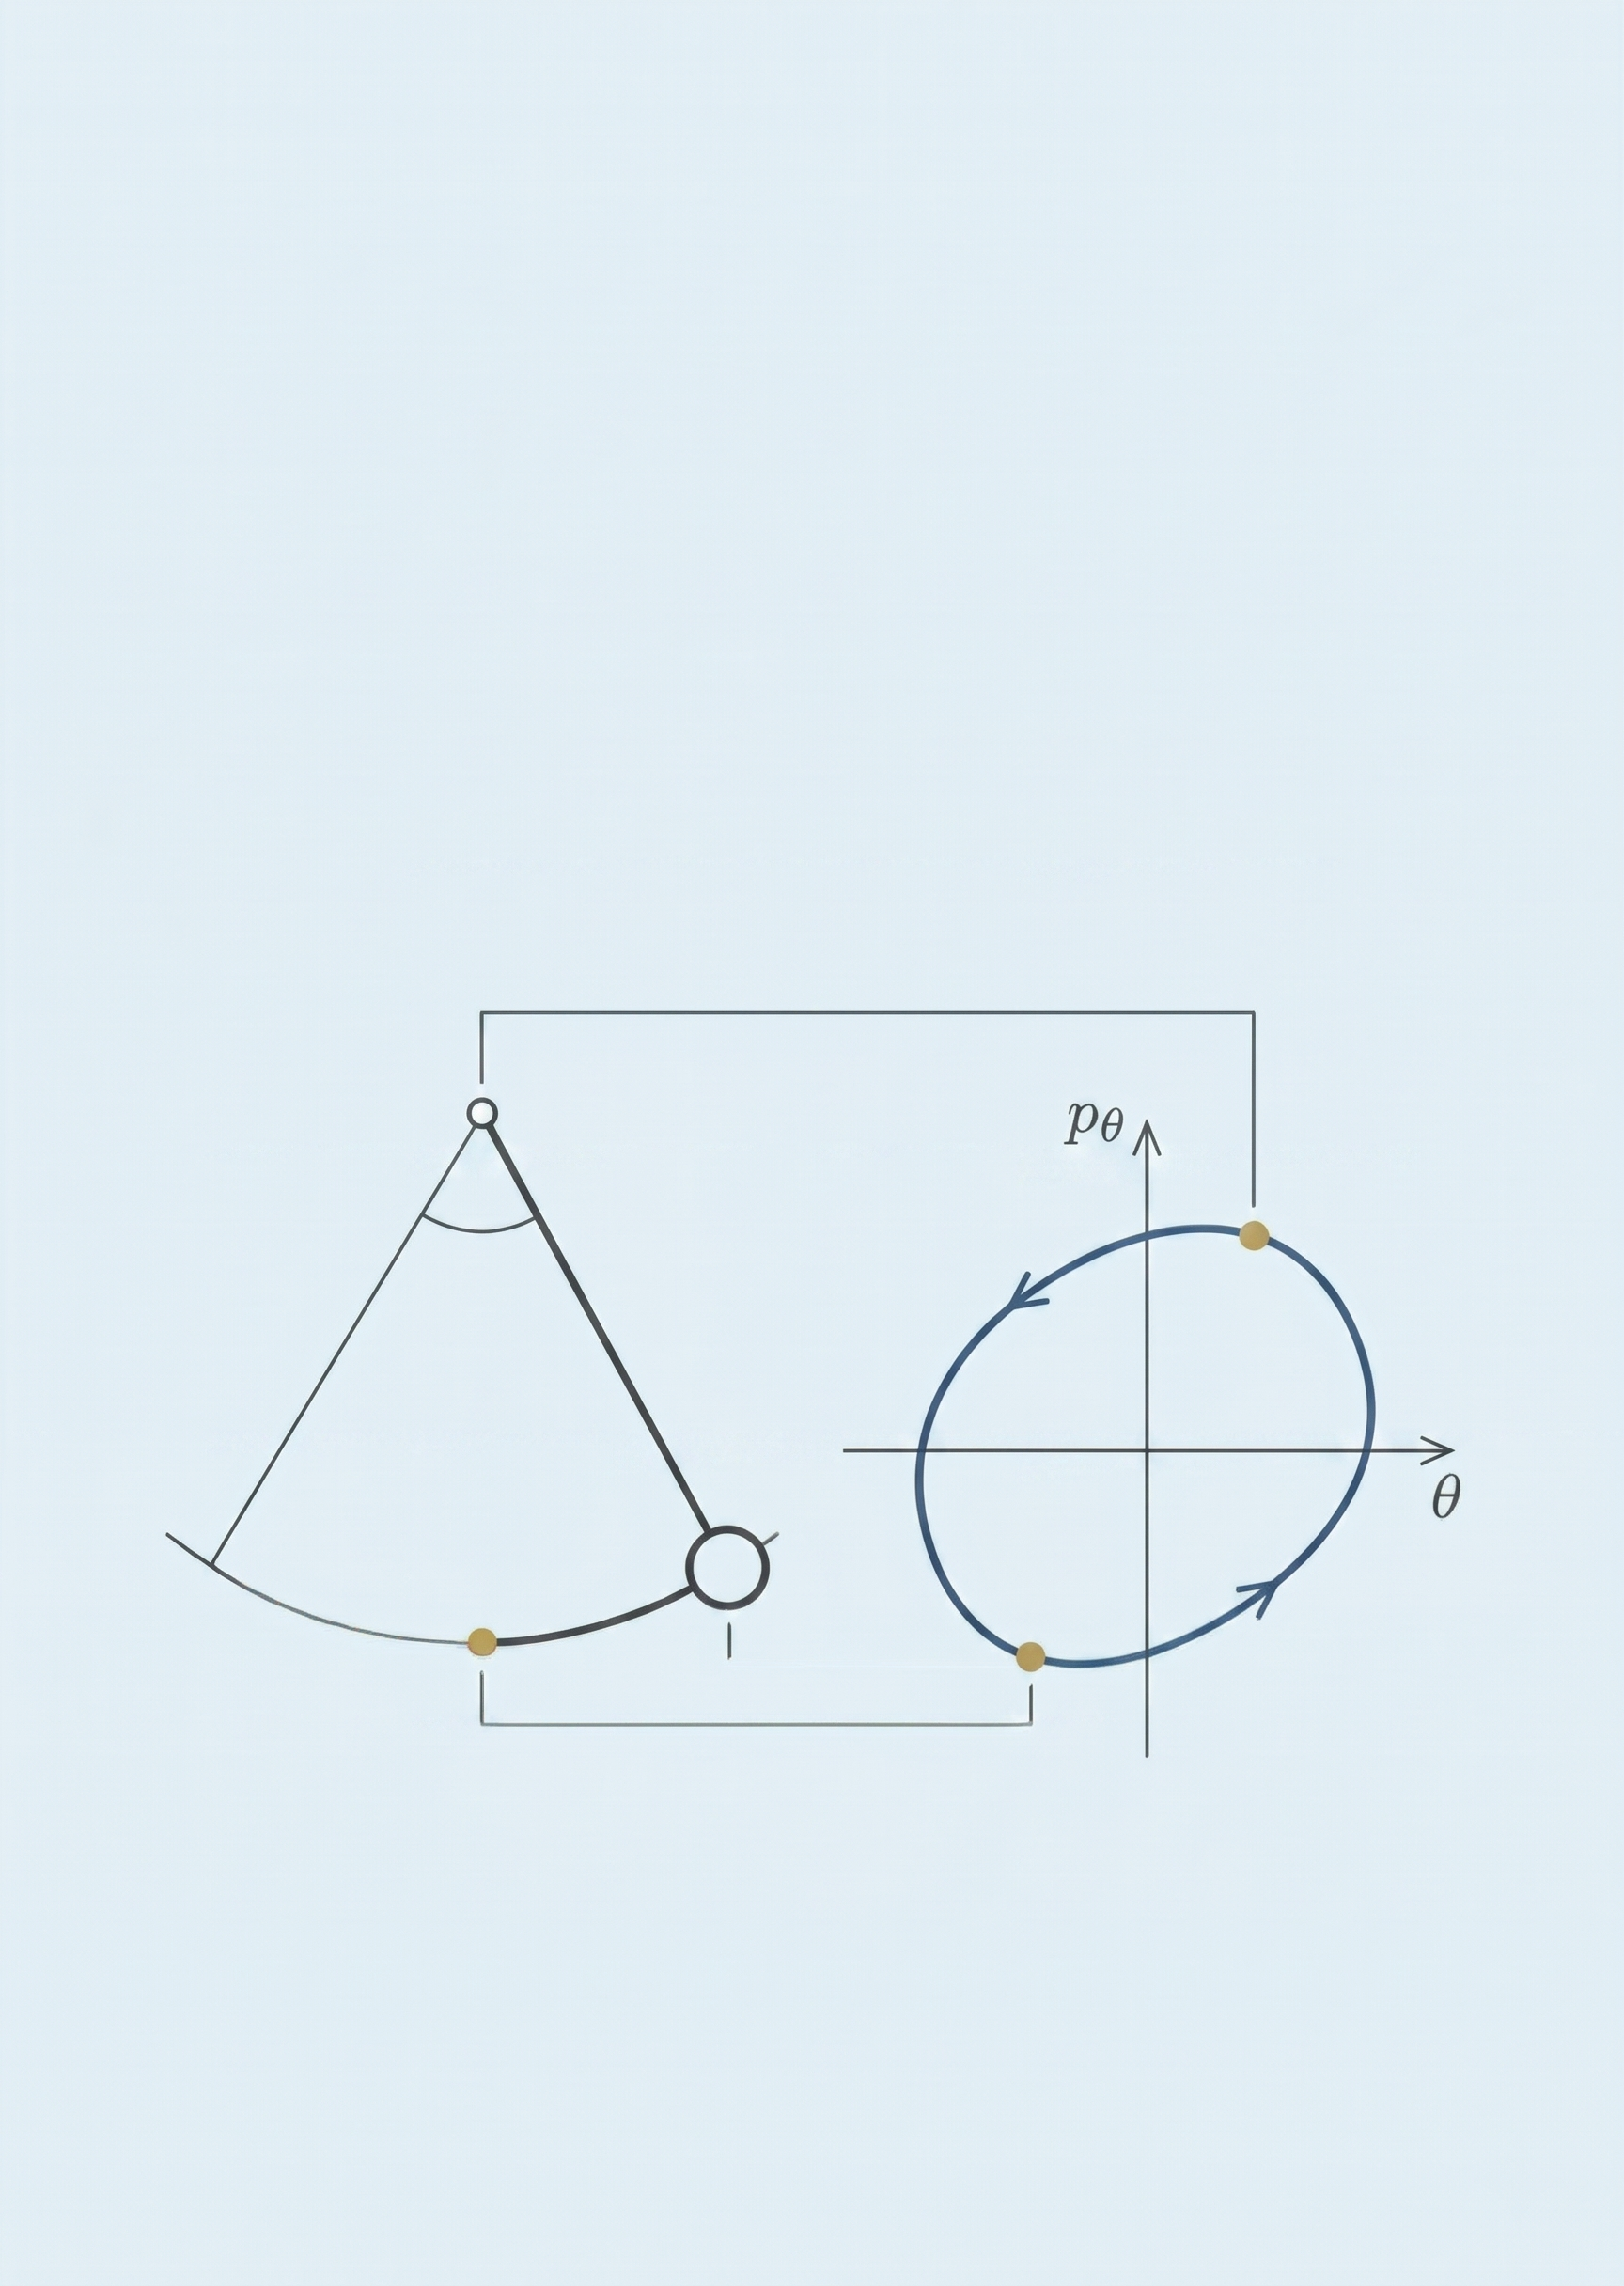
\includegraphics[height=\paperheight,keepaspectratio]{../../../generated_course_notes/core/classical_mechanics/2011_fall_theoretical_minimum/assets/cover-art.png}%
  };
  \node[
    anchor=north west,
    align=left,
    text width=0.78\paperwidth,
    fill=white,
    fill opacity=0.9,
    rounded corners=8pt,
    inner xsep=10pt,
    inner ysep=8pt
  ] at ([xshift=0.08\paperwidth,yshift=-0.06\paperheight]current page.north west) {%
    {\fontsize{30}{33}\selectfont\bfseries\color{black!88} 고전역학\\[0.85em]}
    {\large\color{black!72} 한국어판 / 2011년 가을 · 이론적 최소한}
  };
  \node[
    anchor=south west,
    align=left,
    text width=0.68\paperwidth,
    fill=white,
    fill opacity=0.82,
    text opacity=1,
    rounded corners=6pt,
    inner sep=12pt
  ] at ([xshift=0.08\paperwidth,yshift=0.08\paperheight]current page.south west) {%
    {\normalsize\color{black!78} 원 강의: Leonard Susskind\\[0.35em]}
    {\small\color{black!72} 보조 강의 노트: \href{https://lazying.art}{LazyingArt LLC} / \href{https://github.com/lachlanchen/Video2Book}{Video2Book}}
  };
\end{tikzpicture}
\mbox{}
\end{titlepage}
\hypersetup{pageanchor=true}

\clearpage
\chapter{이 노트에 관하여}
이 동반 노트는 Leonard Susskind의 강의를 바탕으로 독립적으로 편집한 것입니다. 기계 전사본과 자막, 선별한 칠판 영상 프레임을 바탕으로 재구성한 뒤, 이용 가능한 원자료와 대조해 확인했습니다. 이 노트는 Susskind 교수가 직접 작성한 원고가 아니며, 교수의 검토나 승인을 받은 것도 아닙니다.

이 판본은 오픈 소스 \href{https://lazying.art}{LazyingArt LLC}의 \href{https://github.com/lachlanchen/Video2Book}{Video2Book} 워크플로를 사용해 제작했습니다. 기계 전사본은 별도로 제공되며 인식 오류가 있을 수 있습니다. 편집상 명확히 한 부분과 상당한 재구성이 이루어진 부분은 각주에 표시했습니다.
\clearpage
\tableofcontents
\mainmatter
\chapter{상태, 가역성, 운동학}

고전역학은 낙하하는 물체, 공전하는 행성, 대전 입자에 관한 방정식만 모아 놓은 학문이 아니다. 특정한 방정식을 고르기에 앞서, 운동 법칙이 고전 법칙으로 인정되려면 어떤 형태여야 하는지 더 일반적인 질문을 던질 수 있다. 가능한 모든 역사를 칠판에 그려 볼 수 있을 만큼 단순한 계부터 살펴보자. 그런 계에서 상태, 결정론, 가역성, 보존의 개념을 분명히 한 뒤, 일상적인 공간을 움직이는 입자로 돌아오겠다.

\section{두 가지 질문}

역학에는 두 가지 질문이 있다. 하나는 특정한 계를 지배하는 구체적인 법칙을 묻는다. 거대한 물체의 중력장 속에서 움직이는 행성은 한 법칙을 따르고, 자기장 속에서 움직이는 전하 입자는 다른 법칙을 따른다. 이는 자연의 세부 법칙에 관한 질문이다.

다른 질문은 이런 모든 사례에 공통된 틀에 관한 것이다. 허용 가능한 모든 법칙이 따라야 하는 규칙이 있는가? 연구 대상인 힘이나 물체와 무관하게 고전역학 자체에 속하는 특징은 무엇인가? 구체적인 사례들이 답을 보여 주겠지만, 이 두 번째 질문이 학문의 체계를 이룬다.

가장 유용한 첫 사례는 추상적인 탁자 위의 추상적인 동전이다. 동전의 성질 가운데 하나만 남긴다. 앞면이나 뒷면이 나올 수 있다는 성질이다. 따라서 가능한 배치들의 공간은
\begin{equation}
  \mathcal C=\{H,T\}.
\end{equation}
여기서 \emph{배치}란 계가 취할 수 있는 가능한 상태 가운데 하나를 뜻한다. 초기 조건은 그중 하나를 선택하는 것이다. 한쪽 면만 있는 동전은 더 단순하겠지만, 배치가 하나뿐이라 아무 일도 일어날 수 없다. 두 상태면 동역학이 가능해진다.

\section{동전: 상태, 법칙, 역사}

마치 세계가 스트로보스코프로 비추는 것처럼 시간을 정수 단계로 진행시키자:
\begin{equation}
  t=\ldots,-2,-1,0,1,2,\ldots .
\end{equation}
운동 법칙은 갱신 규칙이다. 이 규칙은 시간 \(t\)의 상태에 시간 \(t+1\)의 상태를 대응시킨다. 가장 단순한 규칙은 아무것도 바꾸지 않는다:
\begin{equation}
  H\longmapsto H,
  \qquad
  T\longmapsto T.
  \label{eq:coin-identity}
\end{equation}
\(H\)에서 시작하면 전체 역사는 \(H,H,H,\ldots\)이고, \(T\)에서 시작하면 \(T,T,T,\ldots\)이다. 이 규칙은 재미없지만 완전히 예측 가능하다.

다른 가역 규칙은 두 상태를 맞바꾼다:
\begin{equation}
  H\longmapsto T,
  \qquad
  T\longmapsto H.
  \label{eq:coin-flip}
\end{equation}
이제 역사는 번갈아 나타난다:
\begin{equation}
  H,T,H,T,\ldots,
  \qquad
  T,H,T,H,\ldots .
\end{equation}
화살표는 갱신 전 상태에서 갱신 후 상태로 향한다. 따라서 화살표의 꼬리는 계가 어디서 시작하는지를, 화살촉은 어디로 가는지를 나타낸다.

\begin{figure}[htbp]
  \centering
  \includegraphics[width=0.86\textwidth]{lecture_01_figure_02.png}
  \caption{동전의 두 배치와 방향이 표시된 뒤집기 법칙을 강의 칠판에 그린 그림. 깔끔하게 정리한 갱신 규칙은 식 ~\eqref{eq:coin-flip}에 제시되어 있다.}
  \lectureframe{00:06:50}
  \label{fig:coin-board}
\end{figure}

면을 두 값만 갖는 변수로 나타낼 수 있다,
\begin{equation}
  \sigma=
  \begin{cases}
    +1,&H,\\
    -1,&T.
  \end{cases}
\end{equation}
물리학에서는 두 값만 갖는 양을 나타낼 때 전통적으로 \(\sigma\)를 쓴다. 특히 스핀을 설명할 때 그렇지만, 여기서는 스핀에 관한 지식이 필요하지 않다. 이 표기법을 쓰면 두 규칙은 운동 방정식이 된다:
\begin{align}
  \sigma(t+1)&=\sigma(t),
  &&\text{identity law},\label{eq:sigma-identity}\\
  \sigma(t+1)&=-\sigma(t),
  &&\text{flip law}.\label{eq:sigma-flip}
\end{align}
이 변수는 새로운 물리를 더하지 않는다. 배치를 간결하게 표시하고 그래프를 방정식으로 나타내게 해 준다.

\begin{figure}[htbp]
  \centering
  \includegraphics[width=0.86\textwidth]{lecture_01_figure_03.png}
  \caption{뒤집기 법칙을 \(\sigma(t+1)=-\sigma(t)\)로 나타냈다. 상자 안의 값 \(\sigma=\pm1\)은 앞면과 뒷면을 표시한다.}
  \lectureframe{00:08:58}
  \label{fig:sigma-board}
\end{figure}

어느 규칙에서든 초기 상태와 법칙을 알면 이후 모든 시점의 상태가 정해진다. 이 진술은 계가 \emph{닫혀 있음}을 전제로 한다. 누군가 손을 뻗어 동전을 돌리면, 그 손은 우리의 기술에 포함되지 않은 외부 영향이다. 결정론을 반증한 것이 아니라 계를 바꾼 것이다. 고전 법칙은 계의 시간 변화에 관련된 모든 영향을 포함한 닫힌 계를 지배하도록 정식화된다.

두 원소 집합에서 자기 자신으로 가는 수학적 함수는 네 가지다. 위에 쓰지 않은 나머지 두 함수는 두 입력 모두를 \(H\)에, 또는 두 입력 모두를 \(T\)에 대응시킨다. 이 함수들은 미래 방향으로는 결정론적이지만, 가능한 두 과거의 구별을 없앤다. 아래에서 가역성을 요구하면 식 ~\eqref{eq:coin-identity}과 \eqref{eq:coin-flip}가 허용되는 정확히 두 사상이 된다.

\section{주사위: 궤도와 보존량}

동전을 주사위로 바꾸자. 여기서 주사위에 관해 중요한 사실은 가능한 배치가 여섯 가지라는 점뿐이다,
\begin{equation}
  \mathcal C=\{1,2,3,4,5,6\}.
\end{equation}
초기 조건은 숫자 하나를 고르는 것이다. 다시 모든 상태를 그대로 두는 규칙을 택할 수도 있지만, 덜 단순한 규칙을 살펴볼 때는 방향 그래프가 더 유용하다. 다음을 보자:
\begin{equation}
  1\longmapsto2\longmapsto3\longmapsto4
  \longmapsto5\longmapsto6\longmapsto1.
  \label{eq:six-cycle}
\end{equation}
예를 들어 \(4\)에서 시작하면 역사는 다음과 같다.

\[
  4,5,6,1,2,3,4,\ldots .
\]
여섯 상태가 하나의 순환을 이룬다.\footnote{자료 주: 화살표를 처음 읽을 때 한 구절에서는 \(6\)가 \(6\)로 돌아온다고 말한다. 바로 뒤의 구절과 그려진 순환, 나열된 역사는 모두 의도된 갱신 규칙 \(6\mapsto1\)을 나타낸다.}

\begin{figure}[htbp]
  \centering
  \includegraphics[width=0.86\textwidth]{lecture_01_figure_06.png}
  \caption{여섯 상태가 이루는 하나의 순환. 스트로보스코프의 각 단계마다 상태가 다음 상태로 옮겨 가며, 여섯 번 갱신한 뒤 처음으로 돌아온다.}
  \lectureframe{00:12:40}
  \label{fig:six-cycle-board}
\end{figure}

규칙은 더 복잡해 보일 수 있지만 구조적으로는 달라지지 않을 수 있다. 예를 들어
\begin{equation}
  1\to2\to5\to3\to4\to6\to1
  \label{eq:relabeled-cycle}
\end{equation}
이 규칙도 여전히 하나의 여섯 상태 순환이다. 꼭짓점을 \(1,2,5,3,4,6\) 순서로 페이지 둘레에 배치하면 식 ~\eqref{eq:six-cycle}와 같은 그림이 된다. \(1\)이나 \(5\) 같은 표지는 이름일 뿐이며, 순환 구조는 그 이름에 좌우되지 않는다.

실제로 다른 법칙은 여섯 상태를 두 순환으로 나눈다. 예를 들면
\begin{equation}
  1\to2\to3\to1,
  \qquad
  4\to6\to5\to4.
  \label{eq:two-cycles}
\end{equation}
주사위 하나와 법칙 하나는 그대로지만, 한 순환에서 시작한 궤적은 다른 순환에 절대 도달할 수 없다. 순환마다 숫자 \(Q\)를 붙일 수 있다:
\begin{equation}
  Q=
  \begin{cases}
    0,&\text{on the cycle }\{1,2,3\},\\
    1,&\text{on the cycle }\{4,5,6\}.
  \end{cases}
\end{equation}
상태는 매 단계 바뀌지만 \(Q\)는 바뀌지 않는다.

\begin{definition}
보존량은 운동 법칙에 따라 값이 바뀌지 않는 상태의 함수다.
\end{definition}

같은 생각으로 고정점 하나, 두 상태 순환 하나, 세 상태 순환 하나를 둘 수도 있다. 보존되는 표지는 계가 어느 궤도에 있는지를 나타내지만, 그 궤도 안에서 어떤 상태인지는 알려 주지 않아도 된다. 따라서 보존은 운동과 양립한다. 보존되는 것이 반드시 전체 배치일 필요는 없으며, 가능한 배치들 사이의 어떤 구별만 보존될 수도 있다.

\begin{figure}[htbp]
  \centering
  \includegraphics[width=0.86\textwidth]{lecture_01_figure_07.png}
  \caption{칠판에 그린 서로 분리된 여러 순환: 고정점, 두 상태 순환, 세 상태 순환. 상태가 순환을 따라 움직이는 동안에도 순환 표지는 보존된다.}
  \lectureframe{00:18:40}
  \label{fig:conserved-cycles-board}
\end{figure}

유한한 가역계에서는 모든 궤적이 순환이다. 하나의 순환에서는 궤적이 결국 모든 상태를 방문하므로, 이 기초적인 의미에서 비상수 보존 표지를 둘 수 없다. 여러 순환이 있으면 상태가 한 구성 요소에서 다른 구성 요소로 이동하지 않기 때문에 그런 표지를 둘 수 있다.

\section{상태에 무엇을 포함해야 하는가?}

동전 사례에서는 다음 면이 현재 면에만 의존하는 한 단계 규칙을 사용했다. 청중의 질문 하나가 이러한 제한이 꼭 필요한지 살펴본다.

\begin{classroomqa}
\audiencequestion{다음 결과가 바로 눈에 보이는 면을 넘어, 이전 결과 한 번이나 여러 번에 의존하는 앞면과 뒷면의 수열을 만들 수 있을까요?\lecturetimestamp{00:19:27--00:21:23}}

\lecturerresponse{그렇다. 그런 경우 \(H\)이나 \(T\)만으로는 완전한 상태가 아니다. 이전 면 하나가 필요하다면 상태 공간을 다음과 같이 확장하면 된다:
\(
  \{HH,HT,TH,TT\}.
\)
순서쌍 하나하나는 현재 면과 그 직전 면을 기록한다. 그러면 이 네 상태 공간에서 한 단계 규칙으로 다시 시간 변화를 나타낼 수 있다. 더 많은 과거 정보가 필요하다면 그것도 포함하면 된다.}
\end{classroomqa}

이 답변은 상태의 조작적 의미를 알려 준다.

\begin{definition}
한 시점에서 계의 상태란 운동 법칙과 함께 계의 미래를 예측하는 데 필요한 모든 정보로 이루어진다.
\end{definition}

그러므로 상태는 단순한 사진이 아니다. 시간 변화를 확정하는 완전한 자료 전체가 상태다. 나중에 뉴턴 입자를 기술할 때는 위치만으로 충분하지 않고, 초기 자료에 속도도 포함되어야 한다. 기억을 가진 동전은 같은 원리를 가장 단순하게 보여 주는 사례다.

\section{무한 상태 공간}

상태가 무한히 많다고 해서 물체가 무한히 많이 필요한 것은 아니다. 무한한 직선 위의 정수 격자점들에 갇힌 입자 하나를 생각하자. 입자의 상태는 정수다
\[
  n\in\mathbb Z.
\]
한 법칙은 매 단계 입자를 오른쪽으로 한 칸씩 움직인다:
\begin{equation}
  n(t+1)=n(t)+1.
  \label{eq:lattice-one}
\end{equation}
이 궤도는 닫히지 않지만, 미래와 과거 양쪽으로 계속 따라가면 모든 정수를 지난다. 이런 확장된 의미에서 이 궤도는 끝없이 이어지는 하나의 순환 역할을 한다.

다른 법칙은 한 번에 두 칸씩 움직인다:
\begin{equation}
  n(t+1)=n(t)+2.
  \label{eq:lattice-two}
\end{equation}
이제 짝수 상태는 짝수 상태만 거쳐 변하고, 홀수 상태는 홀수 상태만 거쳐 변한다. 홀짝성이 보존된다:
\begin{equation}
  \begin{aligned}
    Q_{\rm parity}(n)&=n\bmod 2,\\
    Q_{\rm parity}(n(t+1))&=Q_{\rm parity}(n(t)).
  \end{aligned}
\end{equation}
유한 상태 공간에서 무한 상태 공간으로 넘어가면 반복되지 않는 역사가 가능해지지만, 상태, 궤도, 보존의 의미는 달라지지 않는다.

\section{결정론만으로 가역성이 보장되지는 않는다}

이제 미래를 유일하게 예측하지만 고전역학의 두 번째 요건은 만족하지 않는 규칙을 그려 보자. 세 면 동전의 상태를 앞면, 뒷면, 모서리로 두고 다음과 같이 정의하자:
\begin{equation}
  H\to T,
  \qquad
  T\to E,
  \qquad
  E\to T.
  \label{eq:nonreversible-map}
\end{equation}
\(H\)에서 시작하면 역사는
\[
  H,T,E,T,E,\ldots;
\]
이 된다. \(T\)나 \(E\)에서 시작해도 그 뒤의 교대는 마찬가지로 모호하지 않다. 각 상태에서 나가는 화살표가 정확히 하나이므로, 이 규칙은 미래 방향으로 결정론적이다.

현재 상태에서 과거를 되짚으려 할 때 문제가 생긴다. 현재 상태가 \(T\)이라면 직전 상태는 \(H\)일 수도 \(E\)일 수도 있다. 두 역사가 합쳐진 것이다. 모든 화살표의 방향을 뒤집으면 결함이 바로 드러난다. \(T\)에서 역방향 그래프는 두 가지 이동을 허용한다. 역방향 규칙은 결정론적이지 않다.

\begin{figure}[htbp]
  \centering
  \includegraphics[width=0.86\textwidth]{lecture_01_figure_08.png}
  \caption{가역적이지 않은 \(H,T,E\) 규칙과 대표적인 역사들. \(H\)와 \(E\)가 모두 \(T\)로 이어지므로, 현재 상태만으로는 과거를 하나로 정할 수 없다.}
  \lectureframe{00:28:50}
  \label{fig:nonreversible-board}
\end{figure}

\begin{definition}이산 법칙이 가역적이려면 현재 상태가 유일한 다음 상태와 유일한 이전 상태를 모두 결정해야 한다. 상태 그래프에서는 각 상태에서 나가는 화살표와 들어오는 화살표가 각각 정확히 하나씩 있어야 한다.
\end{definition}

유한 상태 공간에서 가역 갱신은 상태들의 순열이다. 상태들 사이의 구별을 새로 만들거나 없애지 않고, 그저 재배열한다. 그래서 그래프가 순환들로 분해된다. 식 ~\eqref{eq:nonreversible-map}의 사상은 함수이지만 일대일 함수는 아니므로 역함수가 없다.

\begin{classroomqa}
\audiencequestion{입자의 확률을 나타내는 상태라면 이런 종류의 규칙을 허용할 수 있을까요?\lecturetimestamp{00:29:46--00:31:17}}

\lecturerresponse{그렇다면 다른 틀이 된다. 여기서 정식화한 근본적인 고전역학은 확률적 갱신 규칙이 아니라 결정론적 법칙을 사용한다. 그런 규칙을 만들어 연구하는 것은 물론 가능하지만, 이 의미에서 고전역학 법칙이라고 하지는 않는다. 양자역학은 같은 의미에서 결정론적이지 않으면서도 가역적 시간 변화에 해당하는 성질을 가지며, 이는 나중에 따로 논의해야 한다. 고전 통계역학도 확률을 사용하지만, 그 출발점은 기저에 있는 역학 법칙이며, 확률은 초기 자료에 대한 불완전한 지식을 나타낸다.}
\end{classroomqa}

이 구별은 중요하다. 정확한 고전 상태를 알지 못해 사용하는 확률분포는 비결정론적 운동 법칙이 아니다. 그것은 미시적 시간 변화가 여전히 결정론적이고 가역적이라고 보는 계에 관해 우리가 가진 정보를 나타낸다.

\section{정확한 법칙과 불완전한 지식}

예측에는 두 가지 요소가 필요하다:
\begin{enumerate}
  \item 운동 법칙;
  \item 초기 상태.
\end{enumerate}
정확한 법칙이 있어도 초기 조건을 근사적으로만 알면 정확한 예측을 얻을 수 없다. 동전의 경우 탁자를 보고 면을 정확히 알아내는 일을 쉽게 상상할 수 있다. 실제 역학 변수는 연속적이다. 위치와 속도는 임의의 실숫값을 취할 수 있으며, 측정으로 소수점 아래 자릿수를 무한히 알아낼 수는 없다.

실제 초기 상태가 가능한 상태들의 작은 영역 안에 있다고 하자. 어떤 동역학에서는 그 영역이 오랫동안 작게 유지되지만, 다른 동역학에서는 서로 가까운 초기 상태들이 빠르게 벌어진다. 혼돈계에서는 초기 상태의 작은 불확실성이 결국 큰 차이로 자란다. 대기가 익숙한 사례다. 측정이 더 정확하면 유용한 예측 기간을 늘릴 수 있지만, 측정 정확도가 아무리 정해져 있어도 예측을 신뢰할 수 없게 되는 시점은 충분히 먼 미래에 반드시 온다.

이러한 실제적 한계가 방정식에 모호성을 끌어들이는 것은 아니다. 초기 조건을 정확히 안다면 고전적인 가역 법칙은 미래와 과거를 모두 결정한다. 정밀도가 유한할 때 정량적으로 물어야 할 것은 다음이다. 주어진 기간 동안 예측하려면 초기 상태를 얼마나 정확히 알아야 하는가?

이제 그래프를 이용한 검사는 간결한 결론을 준다. 모든 상태에서 들어오는 화살표와 나가는 화살표가 하나씩 있는 법칙은 결정론적이며 가역적이다. 입자에 관한 대응되는 진술은 이보다 덜 단순하지만, 같은 고전적 구조를 나타낸다.

\section{추상적 상태에서 공간상의 점으로}

이제 동전과 주사위에서 점입자로 넘어가자. 입자는 1차원, 3차원, 5차원 또는 다른 임의의 차원에서 움직일 수 있지만, 보통의 공간이 곧바로 떠올릴 수 있는 사례다. 점을 정량적으로 기술하려면 다음을 정한다:
\begin{itemize}
  \item 원점;
  \item 서로 수직인 세 축;
  \item 그 축들의 방향;
  \item 길이의 단위.
\end{itemize}
원점은 관례로 정한다. 팔로앨토나 다른 어느 곳에 두어도 되며, 물리적 결론은 그 선택에 좌우되지 않아야 한다. 축은 \(x,y,z\) 또는 \(x_1,x_2,x_3\)으로 표기할 수 있다. \(x\) 방향과 \(y\) 방향을 정한 뒤에는 \(z\)축이 서로 수직인 두 방향 가운데 어느 쪽을 향하게 할 수도 있다. 오른손 좌표계를 택하자. 오른손 엄지를 \(x\) 방향으로, 검지를 \(y\) 방향으로 뻗으면 중지가 \(z\) 방향을 가리키도록 한다.

축 위에 같은 간격의 눈금을 표시하려면 미터, 피트, 인치, 광년 같은 단위가 필요하다. 이런 관례를 정하고 나면 모든 점을 세 수로 표시할 수 있다,
\begin{equation}
  (x,y,z).
\end{equation}
원점에서 세 축을 따라 변위하면 해당 점에 도달할 수 있다. 입자가 여러 개인 계를 기술하려면 입자마다 이런 삼중항 하나가 필요하다.

\begin{figure}[htbp]
  \centering
  \includegraphics[width=0.86\textwidth]{lecture_01_figure_09.png}
  \caption{데카르트 좌표축과 점의 세 좌표. 그림은 좌표 관례를 정한다. 점 자체는 원점과 축을 어디에 두기로 했는지에 좌우되지 않는다.}
  \lectureframe{00:43:00}
  \label{fig:coordinates-board}
\end{figure}

\section{벡터와 그 성분}

벡터는 크기와 방향을 가진 대상이다. 원점에서 한 점까지의 변위는 벡터지만, 벡터는 속도, 가속도, 전기장과 그 밖의 여러 물리량도 나타낸다. 벡터는 \(\mathbf v\)처럼 굵은 글씨로 쓰고, 크기는 \(\lvert\mathbf v\rvert\)로 쓴다. 크기는 음이 아닌 값이며 영벡터일 때에만 0이 된다.

기하학적으로 벡터는 자유롭게 옮길 수 있는 화살표다. 화살표의 길이와 방향을 바꾸지 않고 평행이동해도 벡터는 변하지 않는다. 특정한 문제에서는 벡터를 점에 붙여 나타낼 수 있다. 예를 들어 주어진 위치에서의 전기장을 지정할 때가 그렇다. 하지만 점에 붙어 있다는 것은 추가 정보이지, 추상적 벡터 자체에 속하는 성질은 아니다.

데카르트 좌표축을 기준으로 하면 벡터의 성분은 다음과 같다:
\begin{equation}
  \mathbf v=(v_x,v_y,v_z).
\end{equation}
성분은 축에 사영하여 얻는 부호 있는 수다. 성분은 크기와 방향을 모두 나타낸다. 3차원 피타고라스 정리에 따라
\begin{equation}
  \lvert\mathbf v\rvert^2
  =v_x^2+v_y^2+v_z^2,
  \qquad
  \lvert\mathbf v\rvert
  =\sqrt{v_x^2+v_y^2+v_z^2}.
  \label{eq:vector-magnitude}
\end{equation}
성분들의 비가 방향을 정한다. 성분이 음수라면 벡터가 해당 축의 음의 방향 성분을 가진다는 뜻이다.

\subsection{스칼라배와 벡터 덧셈}

실수배는 벡터의 길이를 바꾸며, 실수가 음수이면 방향도 뒤집는다. \(c>0\)일 때 \(c\mathbf A\)은 \(\mathbf A\)과 같은 방향을 가리키고 크기는 \(c\lvert\mathbf A\rvert\)이다. 특히 \(-\mathbf A\)은 \(\mathbf A\)와 길이가 같고 반대 방향을 가리킨다.

벡터 덧셈을 나타내는 방법은 서로 동등한 세 가지가 있다. 첫째, \(\mathbf B\)의 꼬리를 \(\mathbf A\)의 화살촉에 놓는다. \(\mathbf A\)의 꼬리에서 \(\mathbf B\)의 화살촉으로 향하는 화살표가 \(\mathbf A+\mathbf B\)이다. 둘째, 두 벡터의 꼬리를 한곳에 맞추고 평행사변형을 완성한다. 대각선이 합벡터다. 이 방법에서는 교환법칙이 눈에 드러난다:
\begin{equation}
  \mathbf A+\mathbf B=\mathbf B+\mathbf A.
\end{equation}
셋째, 대응하는 성분끼리 더한다:
\begin{equation}
  C_i=A_i+B_i,
  \qquad i=x,y,z,
  \label{eq:component-addition}
\end{equation}
여기서 \(\mathbf C=\mathbf A+\mathbf B\)이다. 이 규칙들은 \(a\mathbf A+b\mathbf B\) 같은 임의의 선형결합도 정의한다.

\begin{figure}[htbp]
  \centering
  \includegraphics[width=0.86\textwidth]{lecture_01_figure_10.png}
  \caption{벡터 덧셈을 나타내는 삼각형 구성과 평행사변형 구성. 두 구성은 같은 벡터 \(\mathbf A+\mathbf B\)를 준다.}
  \lectureframe{00:53:00}
  \label{fig:vector-addition-board}
\end{figure}

일반적으로 한 벡터를 다른 벡터로 나누는 연산은 없다. 하지만 표준적인 벡터곱은 두 가지가 있다. 벡터곱은 다음 강의에서 다루고, 여기서는 스칼라곱이 필요하다.

\subsection{스칼라곱}

\(\mathbf A\)를 \(\mathbf B\)가 정하는 축에 사영하자. 두 벡터 사이의 각이 \(\theta\)이면, \(\mathbf A\)을 \(\mathbf B\) 방향으로 사영한 부호 있는 성분은 \(\lvert\mathbf A\rvert\cos\theta\)이다. 이 사영값에 \(\lvert\mathbf B\rvert\)을 곱해 다음을 정의한다:
\begin{equation}
  \mathbf A\cdot\mathbf B
  =\lvert\mathbf A\rvert\,\lvert\mathbf B\rvert\cos\theta.
  \label{eq:dot-geometric}
\end{equation}
결과는 다른 벡터가 아니라 스칼라다. 식 ~\eqref{eq:dot-geometric}은 \(\mathbf A\)와 \(\mathbf B\)에 대해 대칭이므로 \(\mathbf A\cdot\mathbf B=\mathbf B\cdot\mathbf A\)이다.

\begin{figure}[htbp]
  \centering
  \includegraphics[width=0.86\textwidth]{lecture_01_figure_11.png}
  \caption{사영을 이용한 스칼라곱의 칠판 구성. 조판된 식은 \(\mathbf A\cdot\mathbf B=AB\cos\theta\)이다.}
  \lectureframe{00:58:30}
  \label{fig:dot-product-board}
\end{figure}

부호에는 기하학적 정보가 담겨 있다. 예각에서는 스칼라곱이 양수이고, 둔각에서는 음수이며, 수직인 벡터에서는 0이다. 따라서
\begin{equation}
  \mathbf A\perp\mathbf B
  \quad\Longleftrightarrow\quad
  \mathbf A\cdot\mathbf B=0
\end{equation}
이며, 벡터는 영벡터가 아니라고 하자.

성분으로 나타내면
\begin{equation}
  \mathbf A\cdot\mathbf B
  =A_xB_x+A_yB_y+A_zB_z.
  \label{eq:dot-components}
\end{equation}
이 식을 사용하면 계산을 바로 할 수 있다. 특히
\begin{equation}
  \mathbf A\cdot\mathbf A
  =A_x^2+A_y^2+A_z^2
  =\lvert\mathbf A\rvert^2.
  \label{eq:self-dot}
\end{equation}
두 벡터의 성분을 알면 식 ~\eqref{eq:dot-geometric}과 \eqref{eq:dot-components}로 두 벡터 사이의 각을 구할 수 있다:
\begin{equation}
  \cos\theta
  =\frac{\mathbf A\cdot\mathbf B}
  {\lvert\mathbf A\rvert\,\lvert\mathbf B\rvert}.
\end{equation}

같은 대수적 계산에서 코사인 법칙이 나온다. \(\mathbf A\)와 \(\mathbf B\)가 삼각형의 한 꼭짓점에서 다른 두 꼭짓점으로 향한다고 하자. 세 번째 변은 \(\mathbf C=\mathbf A-\mathbf B\)이지 \(\mathbf A+\mathbf B\)가 아니다. 따라서
\begin{align}
  C^2
  &=(\mathbf A-\mathbf B)\cdot(\mathbf A-\mathbf B)\notag\\
  &=A^2+B^2-2\mathbf A\cdot\mathbf B\notag\\
  &=A^2+B^2-2AB\cos\theta.
  \label{eq:law-of-cosines}
\end{align}

\begin{figure}[htbp]
  \centering
  \includegraphics[width=0.86\textwidth]{lecture_01_figure_04.png}
  \caption{코사인 법칙을 유도할 때 사용하는 삼각형. 칠판에서 수정한 결과 닫는 변은 \(\mathbf C=\mathbf A-\mathbf B\)로 확인되며, 이에 따라 식 ~\eqref{eq:law-of-cosines}가 나온다.}
  \lectureframe{01:04:29}
  \label{fig:law-cosines-board}
\end{figure}

\section{위치, 속도, 가속도}

원점을 정하고, \(\mathbf r\)를 원점에서 입자까지 향하는 위치 벡터로 두자. 그 성분은 데카르트 좌표다:
\begin{equation}
  \mathbf r=(x,y,z),
  \qquad
  \lvert\mathbf r\rvert=\sqrt{x^2+y^2+z^2}.
\end{equation}
원점을 바꾸면 \(\mathbf r\)가 어떻게 바뀌는지는 뒤에서 다루겠다. 원점을 정한 뒤에는 시간에 따라 변하는 위치로 운동을 기술한다,
\begin{equation}
  \mathbf r(t)=\bigl(x(t),y(t),z(t)\bigr).
\end{equation}
따라서 궤적은 시간의 함수 세 개로 나타난다.

속도는 위치의 시간 미분이다:
\begin{equation}
  \mathbf v(t)=\frac{d\mathbf r}{dt}
  =\dot{\mathbf r}(t),
  \qquad
  v_i=\frac{dx_i}{dt}=\dot x_i.
  \label{eq:velocity}
\end{equation}
점 표기는 언제나 시간에 대한 미분을 뜻한다. 크기 \(\lvert\mathbf v\rvert\)는 속력이다. 일반적으로 위치와 속도는 서로 독립적인 방향을 가진다. 한 위치에 있는 입자는 문제에서 허용하는 어느 방향으로든 움직일 수 있다.

가속도는 속도의 변화율이므로 위치의 이계 시간 미분이다:
\begin{equation}
  \mathbf a(t)=\frac{d\mathbf v}{dt}
  =\dot{\mathbf v}(t)
  =\frac{d^2\mathbf r}{dt^2}
  =\ddot{\mathbf r}(t),
  \qquad
  a_i=\ddot x_i.
  \label{eq:acceleration}
\end{equation}
가속도 역시 벡터다. 양의 \(x\) 방향으로 움직이는 입자의 속력이 증가하면 \(a_x>0\)이다. 속력이 감소하면 \(a_x<0\)이다. 흔히 감속이라고 부르는 것은 현재 속도와 반대 방향인 가속도일 뿐이다. 더 일반적으로는 크기가 일정해도 방향이 바뀌면서 속도가 변할 수 있다.

\begin{figure}[htbp]
  \centering
  \includegraphics[width=0.86\textwidth]{lecture_01_figure_05.png}
  \caption{위치 성분의 시간 미분으로 쓴 속도 성분. 간결한 벡터 표기에서는 \(\mathbf v=d\mathbf r/dt\)이다.}
  \lectureframe{01:14:24}
  \label{fig:velocity-board}
\end{figure}

\subsection{직선 위의 등가속도 운동}

1차원 운동에서는 다음과 같이 쓰자:
\begin{equation}
  x(t)=a+bt+ct^2.
  \label{eq:quadratic-motion}
\end{equation}
\(t=0\)일 때 입자의 위치는 \(x=a\)이다. 한 번, 이어서 두 번 미분하면 다음을 얻는다:
\begin{align}
  v(t)=\dot x(t)&=b+2ct,\label{eq:line-velocity}\\
  a(t)=\ddot x(t)&=2c.\label{eq:line-acceleration}
\end{align}
따라서 \(b\)는 초기 속도이고 \(2c\)는 일정한 가속도다. \(c>0\)이면 속도가 선형적으로 증가하고, \(c<0\)이면 선형적으로 감소한다. 이 이차 위치 법칙은 지표면 근처에서 낙하하는 물체의 이상화된 운동처럼 일정한 가속도 아래에서 나타나는 운동의 형태다.

\section{등속 원운동}

마지막 예로 입자가 단위원 위의 \(x\)-\(y\) 평면에서 움직인다고 하자. 입자는 양의 \(x\)축 위의 \(t=0\)에서 출발하고, 각좌표는 일정한 비율로 증가한다:
\begin{equation}
  \theta(t)=\omega t.
\end{equation}
상수 \(\omega\)은 각진동수다. 한 바퀴 돌면 각도가 \(2\pi\)만큼 증가하므로 주기는
\begin{equation}
  T=\frac{2\pi}{\omega}.
  \label{eq:circular-period}
\end{equation}
이다. 각도가 \(2\pi\)를 넘어 계속 증가하도록 둘 수 있다. 연속적으로 기록하는 각도는 초기화되지 않더라도 위치는 반복된다.

단위원 위에서는
\begin{equation}
  \mathbf r(t)
  =\bigl(\cos\omega t,\,\sin\omega t\bigr).
  \label{eq:circular-position}
\end{equation}
미분하면
\begin{equation}
  \mathbf v(t)
  =\omega\bigl(-\sin\omega t,\,\cos\omega t\bigr).
  \label{eq:circular-velocity}
\end{equation}
속도는 원에 접한다. 그림에 의존하지 않고 반지름과 수직임을 증명할 수 있다:
\begin{align}
  \mathbf r\cdot\mathbf v
  &=\cos\omega t\,(-\omega\sin\omega t)
    +\sin\omega t\,(\omega\cos\omega t)\notag\\
  &=0.
  \label{eq:r-dot-v}
\end{align}

\begin{figure}[htbp]
  \centering
  \includegraphics[width=0.86\textwidth]{lecture_01_figure_12.png}
  \caption{단위원 위 운동에서의 위치 성분과 속도 성분. \(\mathbf r\cdot\mathbf v\)에서 항들이 상쇄됨을 통해 속도가 원에 접함을 확인할 수 있다.}
  \lectureframe{01:24:30}
  \label{fig:circular-velocity-board}
\end{figure}

한 번 더 미분하면
\begin{equation}
  \mathbf a(t)
  =-\omega^2
  \bigl(\cos\omega t,\,\sin\omega t\bigr)
  =-\omega^2\mathbf r(t).
  \label{eq:centripetal-acceleration}
\end{equation}
가속도는 반지름과 평행하지만 반대 방향, 즉 중심 쪽을 향한다. 이것이 구심 가속도다.\footnote{용어 주: 강의의 이 대목에는 ``원심''이라는 단어가 나오지만, 방정식과 함께 제시된 설명은 중심을 향하는 표준적인 구심 가속도를 가리킨다.}

\begin{figure}[H]
  \centering
  \includegraphics[width=0.86\textwidth]{lecture_01_figure_13.png}
  \caption{원운동 가속도의 성분 계산. 각 성분은 해당 위치 성분에 \(-\omega^2\)를 곱한 값이므로 \(\mathbf a=-\omega^2\mathbf r\)이다.}
  \lectureframe{01:26:30}
  \label{fig:circular-acceleration-board}
\end{figure}

반지름이 1이므로
\begin{equation}
  \lvert\mathbf r\rvert=1,
  \qquad
  \lvert\mathbf v\rvert=\omega,
  \qquad
  \lvert\mathbf a\rvert=\omega^2.
\end{equation}
\(\omega\)이 커지면 속력은 선형적으로 증가하고 필요한 안쪽 가속도는 이차적으로 증가한다. 반지름이 \(R\)인 원에서는 같은 계산으로 \(v=\omega R\)과 \(\lvert\mathbf a\rvert=\omega^2R=v^2/R\)를 얻는다. 첫 계산을 간결하게 하기 위해 강의에서는 \(R=1\)로 둔다.

이제 입자역학에 필요한 기초 언어, 즉 상태와 초기 자료, 가역적인 시간 변화, 좌표, 그리고 속도와 가속도를 정의하는 미분을 살펴보았다. 다음 과제는 입자를 규정하는 초기 자료가 정확히 무엇인지 정하고, 그 자료를 한 순간에서 다음 순간으로 옮기는 법칙을 찾는 것이다.\chapter{힘, 위상 공간, 보존 법칙}

\lectureoverview{운동 법칙은 익숙한 물리량 사이의 관계를 제시하는 데 그쳐서는 안 된다. 계의 상태를 명시하고, 그 상태를 한 순간에서 다음 순간으로 옮기며, 운동 중에도 유지되는 구별과 물리량이 무엇인지 밝혀야 한다. 그럴듯하지만 틀린 힘의 법칙을 먼저 검토하고, 상태를 위치에서 위상 공간으로 확장한 뒤, 운동량과 에너지 보존을 유도하여 뉴턴 역학에 도달할 것이다.}

\section{유용한 오답 법칙}

일상적인 운동은 마찰의 영향을 크게 받는다. 무거운 물체를 바닥에서 밀면 움직이지만, 밀기를 멈추면 곧 정지한다. 일반적으로 더 큰 힘을 가하면 더 빠르게 움직이고, 더 무거운 물체를 움직이려면 더 세게 밀어야 한다. 이런 세계에서는 힘이 속도 자체를 만들어 낸다고 생각하기 쉽다. 이것이 아리스토텔레스식 운동 설명의 기본 직관이었다.

빠져 있던 경험은 빙판에서 스케이트를 타면 얻을 수 있다. 스케이터는 출발하거나 멈추거나 방향을 바꾸려면 힘이 필요하지만, 일단 움직이기 시작한 뒤 미끄러져 나아가는 데에는 힘이 필요하지 않다. 아리스토텔레스가 평범한 지면이 아니라 마찰이 거의 없는 얼음 위에서 연구했다면, 힘--속도 직관의 결함을 훨씬 알아차리기 어려웠을 것이다.

그 직관의 무엇이 잘못되었는지 드러내기 위해, 이를 현대적인 형태로 정확히 써 보자. 의도적으로 틀리게 만든 방정식을 다음과 같이 적는다.

\begin{equation}
  \mathbf F=m\mathbf v.
  \label{eq:aristotle-vector-law}
\end{equation}

이것은 뉴턴의 법칙이 아니며 물리 법칙으로 외워서는 안 된다. 이 법칙의 가치는 진단에 있다. 말로 된 규칙을 방정식으로 쓰고 나면, 그 규칙이 운동을 예측하는지, 과거를 재구성하기에 충분한 정보를 보존하는지 물을 수 있다. 힘을 뜻하는 그리스어에 관한 짧은 수업 중 토론은 \emph{dynamis}를 가리킨다. 이 어근은 dynamo나 dynamics 같은 단어에서도 찾아볼 수 있지만, 용어보다 중요한 것은 법칙 자체를 검토하는 일이다.

\begin{figure}[htbp]\centering
  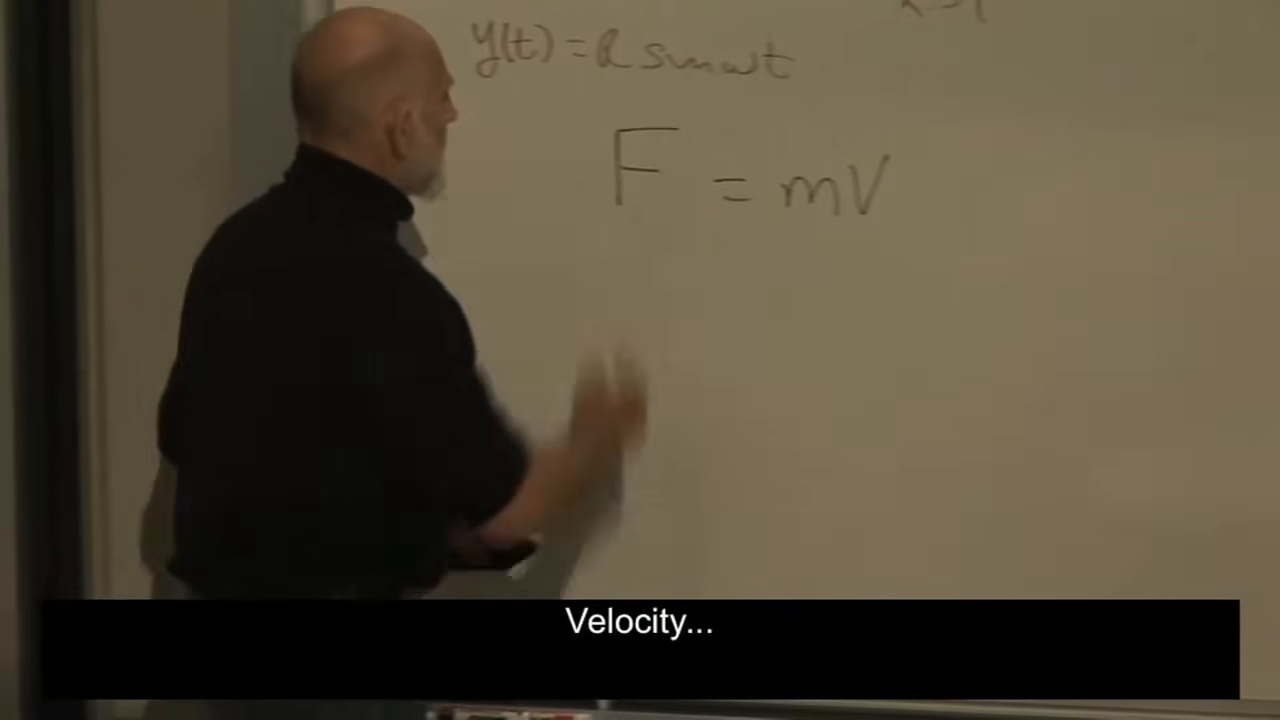
\includegraphics[width=0.82\textwidth]{lecture_02_figure_02.png}\caption{예측 가능성과 가역성을 검토하는 데 쓰는 의도적으로 틀린 힘--속도 법칙.}\lectureframe{00:04:51}\end{figure}

운동을 한 공간 좌표로 제한하자. \(v=\dot x\)이므로, 법칙은 다음과 같다.

\begin{equation}
  F(t)=m\dot x(t).
  \label{eq:aristotle-1d}
\end{equation}

이제 시간을 길이 \(\delta\)인 짧은 구간들로 나누자. 한 구간 동안에는

\begin{equation}
  \dot x(t)\simeq
  \frac{x(t+\delta)-x(t)}{\delta}.
  \label{eq:first-difference}
\end{equation}

식~\eqref{eq:aristotle-1d}에 대입하면

\begin{equation}
  x(t+\delta)
  =x(t)+\frac{\delta}{m}F(t).
  \label{eq:aristotle-update}
\end{equation}

이는 실제적인 갱신 규칙의 형태를 띤다. 현재 위치와 힘을 알면 다음 스트로보스코프 순간의 위치를 구할 수 있다. 그러나 힘이 사라지면 아리스토텔레스의 규칙은 \(\dot x=0\)을 준다. 즉, 물체는 정지 상태를 유지해야 한다. 운동을 지속시키는 힘이 없는 운동은 애초에 배제된다.

\begin{figure}[htbp]\centering
  \includegraphics[width=0.84\textwidth]{lecture_02_figure_07.png}\caption{복원력이 있을 때의 이산 아리스토텔레스 갱신. 각 단계에서 변위는 약간 1보다 작은 인자를 곱한 값이 된다.}\lectureframe{00:10:15}\end{figure}

\subsection{아리스토텔레스 역학에서의 용수철}

평형 위치가 \(x=0\)인 용수철에 연결된 입자를 생각하자. 변위가 생기면 복원력은 다음과 같다.

\begin{equation}
  F(x)=-kx,
  \qquad k>0.
  \label{eq:hooke-law}
\end{equation}

이 힘을 식~\eqref{eq:aristotle-update}에 대입하면

\begin{equation}
  x(t+\delta)
  =\left(1-\frac{k\delta}{m}\right)x(t).
  \label{eq:aristotle-spring-update}
\end{equation}

\(\delta\)가 충분히 작으면 괄호 안의 인자는 1보다 조금 작다. 따라서 매 갱신마다 변위가 같은 비율만큼 줄어든다.

\begin{equation}
  x_n=\left(1-\frac{k\delta}{m}\right)^n x_0.
  \label{eq:aristotle-geometric-decay}
\end{equation}

연속 방정식과 그 해는 다음과 같다.

\begin{align}
  m\dot x&=-kx,
  \label{eq:aristotle-spring-continuous}\\
  x(t)&=x(0)e^{-kt/m}.
  \label{eq:aristotle-spring-solution}
\end{align}

용수철은 진동하지 않는다. 어떤 변위에서 놓아도 원점에 지수적으로 가까워지며, 다가갈수록 점점 느리게 움직인다.

\begin{figure}[htbp]\centering
  \includegraphics[width=0.84\textwidth]{lecture_02_figure_08.png}\caption{아리스토텔레스식 용수철 방정식의 지수 함수 해. 변위는 진동하지 않고 감소한다.}\lectureframe{00:12:02}\end{figure}

미래를 예측하기는 쉽다. 초기 변위가 무엇이든 모두 같은 정지 상태에 가까워진다. 과거는 그렇지 않다. 입자가 유한한 정밀도로 원점 가까이에서 관측되었다고 하자. 지수적으로 작아진 흔적은 결국 모두 같은 측정 오차 범위 안에 들기 때문에, 입자는 서로 다른 여러 변위 중 어느 위치에서든 출발했을 수 있다. 수학적으로 완벽한 정밀도를 가정하면 식~\eqref{eq:aristotle-spring-solution}을 역으로 풀 수 있지만, 서로 다른 이력 사이의 실질적인 구별은 계속 지워진다. 따라서 이 법칙은 가역적인 기본 동역학이라는 관점에서 의심스럽다.

그렇다고 아리스토텔레스가 비합리적이었다는 뜻은 아니다. 그가 설명한 마찰 지배 운동은 실제로 소산적이다. 잘못은 그런 유효한 거동을 기본 법칙으로 격상한 데 있다. 마찰 자체는 복잡한 미시적 상호작용에서 생기는 힘이다. 손으로 물체를 거의 일정한 속도로 밀 때는 가한 힘이 마찰과 균형을 이룬다. 가한 힘이 속도 자체를 만들어 내는 것은 아니다.

\section{뉴턴의 법칙과 그 물리적 의미}

뉴턴 역학에서 바로잡는 핵심은 힘이 운동 상태를 변화시킨다는 것이다.

\begin{equation}
  \mathbf F=m\mathbf a=m\ddot{\mathbf x}.
  \label{eq:newton-second-law}
\end{equation}

이를 운동 방정식으로 다루기 전에, 겉보기에 순환적으로 보이는 두 가지 문제를 풀어야 한다. 첫 번째는 기준계에 관한 문제다. 뉴턴 법칙은 관성계에서 성립하고, 관성계는 뉴턴 법칙이 성립하는 기준계라고들 한다. 물리적 주장은 그런 순환 정의가 아니다. 적절한 막대자와 시계로 기술되는 \emph{실제로 존재하는} 기준계에서 뉴턴 법칙이 간단한 형태를 취한다는 경험적 주장이다. 그 기준계에 대해 가속하거나 회전하는 기준계에서는 겉보기 힘을 추가해야 한다. 그런 다른 기준계에서 방정식이 어떻게 변환되는지는 나중에 다룰 수 있다.

두 번째 순환 문제는 힘과 질량에 관한 것이다. 힘을 질량 곱하기 가속도로 정의하고 질량을 힘 나누기 가속도로 정의하면, 방정식은 아무 내용도 없는 것처럼 보인다. 조작적 실험을 하면 정의와 법칙을 구분할 수 있다. 물체를 표준 킬로그램과 저울에 걸어 비교한 뒤, 다른 힘이 없는 공간에서 그 물체를 용수철 저울에 연결한다. 용수철을 정해진 만큼 조금 늘리는 데 필요한 힘을 힘의 한 단위로 정의하자. 똑같이 늘어난 동일한 용수철 두 개는 힘 두 단위를 제공하고 가속도는 두 배로 만든다. 실제 용수철은 결국 비선형적으로 거동하거나 끊어지므로, 용수철 하나를 두 배로 늘리는 것보다 두 번째 용수철을 더하는 편이 안전하다. 용수철 하나에 같은 질량 두 개를 연결하면 가속도는 절반이 되고, 같은 질량 세 개를 연결하면 3분의 1이 된다.

\begin{figure}[htbp]\centering
  \includegraphics[width=0.84\textwidth]{lecture_02_figure_09.png}\caption{힘의 같은 단위를 정의하고 가속도가 힘에 비례하는지 검토하는 용수철 저울 사고 실험.}\lectureframe{00:22:45}\end{figure}

이 비교를 통해 다음 식에 경험적 의미가 부여된다.

\begin{equation}
  a\propto F,
  \qquad
  a\propto\frac{1}{m},
  \qquad
  F=ma.
  \label{eq:force-mass-scaling}
\end{equation}

\emph{입자}라는 말은 내부 구조가 중요하지 않은 작은 물체를 가리키는 데 쓸 것이다. 여기서 입자는 소립자에만 한정되지 않는다.

\subsection{위치만으로 상태를 나타낼 수 없는 이유}

이제 같은 스트로보스코픽 방법으로 뉴턴 방정식을 검토하자. 가속도를 나타내는 중심 유한차분은 다음과 같다.

\begin{equation}
  \ddot x(t)\simeq
  \frac{x(t+\delta)-2x(t)+x(t-\delta)}{\delta^2}.
  \label{eq:second-difference}
\end{equation}

따라서 뉴턴 방정식은 다음을 함의한다.

\begin{equation}
  x(t+\delta)
  =2x(t)-x(t-\delta)+\frac{\delta^2}{m}F(t).
  \label{eq:newton-position-update}
\end{equation}

다음 위치는 \(x(t)\)만으로 구할 수 없다. 이전 위치 \(x(t-\delta)\), 또는 이에 동등하게 현재 순간의 속도도 알아야 한다. 처음에는 이 때문에 뉴턴 방정식이 아리스토텔레스 법칙보다 예측력이 떨어지는 것처럼 보인다. 그러나 올바른 결론은 위치만으로는 상태를 완전히 기술할 수 없다는 것이다. 어떤 한 순간에 관련된 정보를 모두 안다는 것은 이후 운동을 결정하기에 충분한 자료를 안다는 뜻이다. 뉴턴 입자에서는 위치와 속도가 그 자료에 해당한다.

\section{운동량과 위상 공간}

운동량을 다음과 같이 도입하자.

\begin{equation}
  \mathbf p=m\mathbf v=m\dot{\mathbf x}.
  \label{eq:momentum-definition}
\end{equation}

고정된 뉴턴 계의 질량은 일정하다고 가정한다. 물체의 일부가 떨어져 나갈 수는 있다. 예컨대 펜에서 뚜껑이 떨어져 나갈 수 있지만, 그러면 기술 대상인 물체가 달라진 것이다. 선택한 닫힌 계의 전체 질량은 여전히 일정하다. \(m\)가 일정하면 뉴턴의 제2법칙은 다음과 같이 된다.

\begin{equation}
  \mathbf F=\dot{\mathbf p}.
  \label{eq:newton-momentum-form}
\end{equation}

\begin{figure}[htbp]\centering
  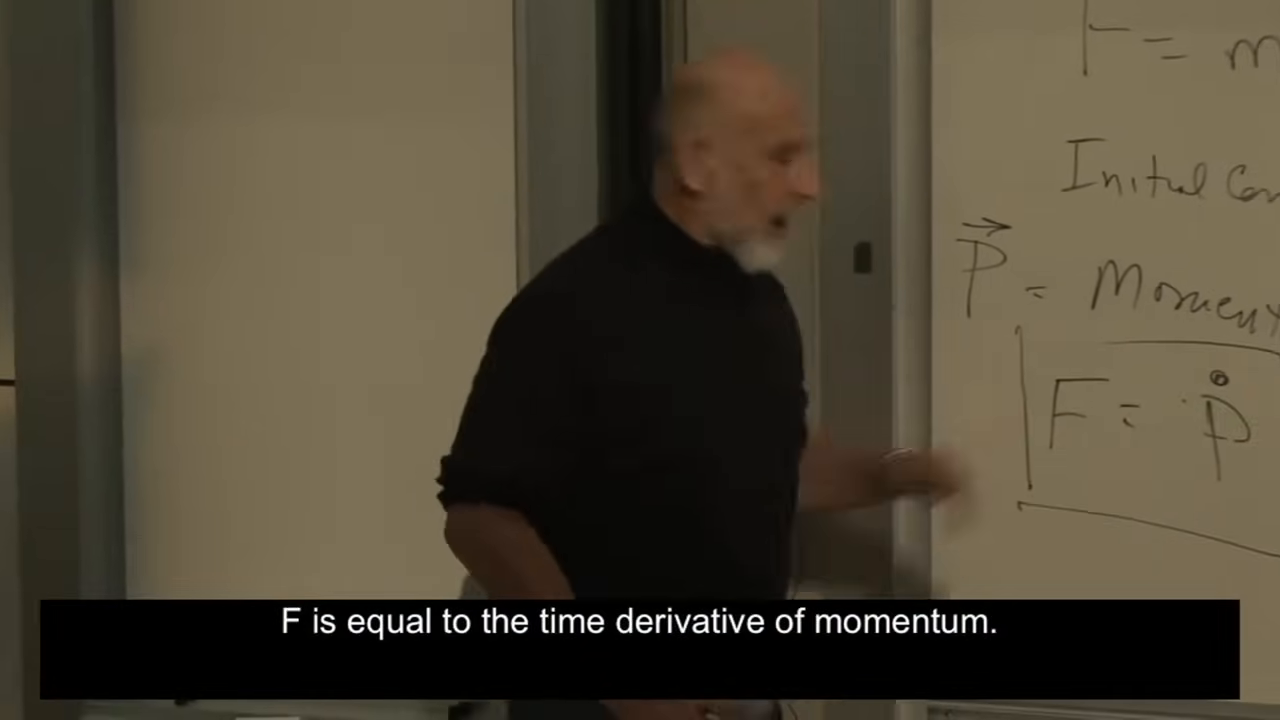
\includegraphics[width=0.82\textwidth]{lecture_02_figure_03.png}\caption{운동량의 시간 미분으로 나타낸 뉴턴의 법칙.}\lectureframe{00:32:35}\end{figure}

한 좌표에서 뉴턴 운동은 서로 독립적인 상태 변수 두 개에 관한 1계 방정식 두 개로 쓸 수 있다.

\begin{align}
  \dot p&=F(x,t),
  \label{eq:first-order-p}\\
  \dot x&=\frac{p}{m}.
  \label{eq:first-order-x}
\end{align}

한 방정식은 힘이 운동량을 어떻게 변화시키는지 말하고, 다른 방정식은 운동량이 위치를 어떻게 변화시키는지 말한다. 이에 대응하는 이산 1계 형태는 다음과 같다.

\begin{align}
  p(t+\delta)&=p(t)+\delta F(x(t),t)+O(\delta^2),
  \label{eq:momentum-discrete}\\
  x(t+\delta)&=x(t)+\frac{\delta}{m}p(t)+O(\delta^2).
  \label{eq:position-discrete}
\end{align}

\(x(t)\)와 \(p(t)\)를 알면, 이 방정식들로 다음 순간의 두 값을 구할 수 있다. 그 값들이 다음 단계의 입력이 된다. 이렇게 갱신을 반복해 궤적을 만든다.

\begin{figure}[htbp]\centering
  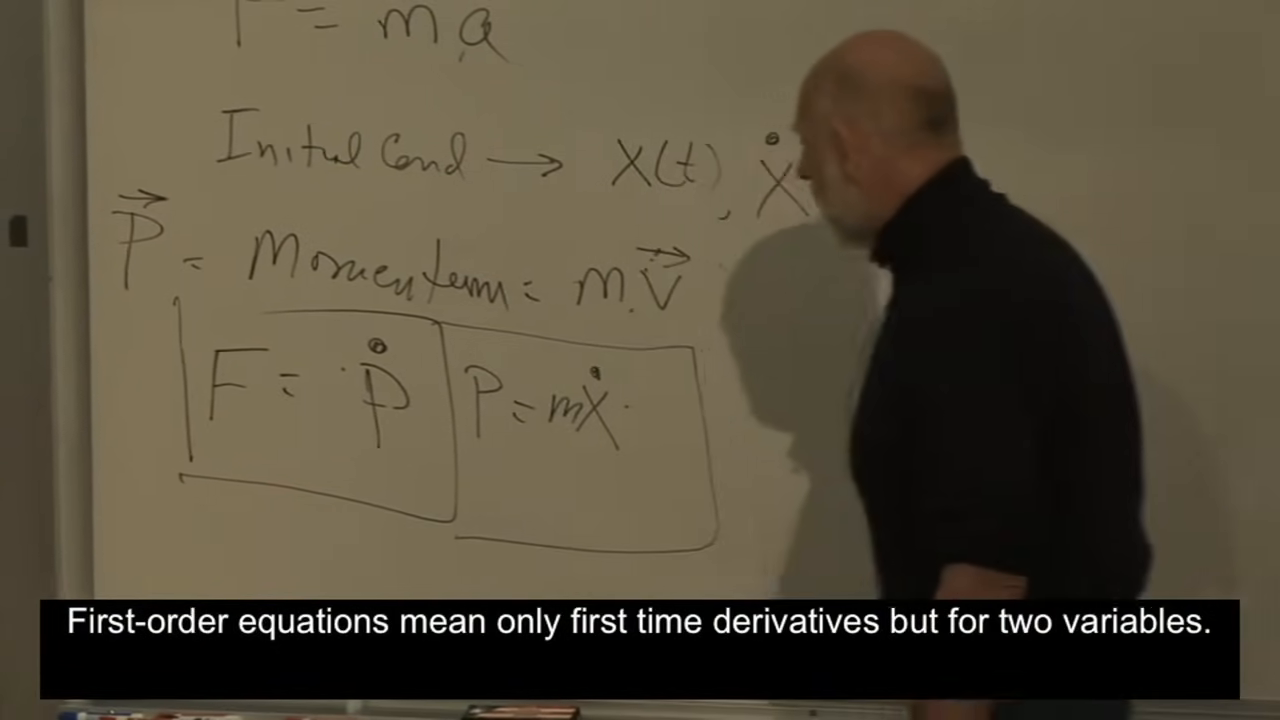
\includegraphics[width=0.84\textwidth]{lecture_02_figure_04.png}\caption{두 개의 1계 방정식과 그에 대응하는 초기 자료. 위치와 운동량을 함께 주면 상태가 정해진다.}\lectureframe{00:35:47}\end{figure}

모든 순서쌍 \((x,p)\)이 이루는 공간을 \emph{위상 공간}이라 한다. 3차원에서 움직이는 입자 하나의 위상 공간은 좌표 여섯 개로 이루어진다.

\begin{equation}
  (x,y,z,p_x,p_y,p_z).
  \label{eq:one-particle-phase-space}
\end{equation}

위상 공간은 완전한 초기 조건들의 공간이다. 배치 공간은 위치만 기록하지만, 위상 공간은 운동 법칙에 필요한 자료를 정확히 기록한다.

\begin{classroomqa}\audiencequestion{힘이 시간에 따라 주어지는 함수가 아니라 위치의 함수라면, 갱신이 더 복잡해지나요?\lecturetimestamp{00:36:27--00:37:07}}\lecturerresponse{방정식은 여전히 운동을 예측한다. \(x\)와 \(p\)를 알면 \(F(x)\)의 값을 안다. 식~\eqref{eq:first-order-p}은 \(p\)를 갱신하고, 식~\eqref{eq:first-order-x}은 \(x\)를 갱신하므로, 갱신된 순서쌍을 다시 사용할 수 있다.}\end{classroomqa}

\section{뉴턴 역학의 용수철}

두 법칙을 같은 물리적 조건에서 비교하기 위해 용수철로 돌아가자. 뉴턴 법칙은 다음과 같다.

\begin{equation}
  m\ddot x=-kx.
  \label{eq:newton-spring}
\end{equation}

상수를 없애기 위해 잠시 \(m=k=1\)로 놓자. 그러면

\begin{equation}
  \ddot x=-x.
  \label{eq:normalized-oscillator}
\end{equation}

지수 함수와 달리 사인과 코사인은 두 번 미분하면 자기 자신에 음수를 곱한 함수가 된다. 일반해는 다음과 같이 쓸 수 있다.

\begin{align}
  x(t)&=C\cos(t-t_0),
  \label{eq:oscillator-x}\\
  p(t)=\dot x(t)&=-C\sin(t-t_0).
  \label{eq:oscillator-p}
\end{align}

두 상수에는 초기 정보 두 가지가 담겨 있다. 진폭 \(C\)은 최대 변위를 나타내고, \(t_0\)은 위상을 정한다. 여기서는 \(t=t_0\)에서 속도가 영이 되도록 위상을 정했다. 입자는 양 끝점에서 순간적으로만 멈춘다. 그런 다음 되돌아와 원점을 지나며, 그곳에서 속력과 운동량이 최대가 되고 계속 진동한다.

식~\eqref{eq:oscillator-x}과 \eqref{eq:oscillator-p}의 양변을 제곱하면 다음과 같다.

\begin{equation}
  x^2+p^2=C^2.
  \label{eq:oscillator-phase-circle}
\end{equation}

따라서 위상 공간의 점은 반지름이 \(C\)인 원을 따라 움직인다. 초기 진폭이 다르면 서로 다른 원이 생기고, \(t_0\)을 바꾸면 같은 원 위에서 출발점이 달라진다. 모든 원은 진폭과 관계없이 이 정규화된 단위계에서 같은 주기 \(2\pi\)로 한 바퀴를 돈다.

\begin{figure}[htbp]\centering
  \includegraphics[width=0.84\textwidth]{lecture_02_figure_10.png}\caption{진동자의 해와 \((x,p)\) 위상 평면에서의 원 궤도.}\lectureframe{00:43:20}\end{figure}

\begin{figure}[htbp]\centering
  \begin{tikzpicture}[scale=1.05,>=Latex]
    \draw[->] (-2.6,0) -- (2.75,0) node[right] {$x$};
    \draw[->] (0,-2.4) -- (0,2.55) node[above] {$p$};
    \draw[blue!65!black,thick] (0,0) circle (1.85);
    \draw[->,blue!65!black,thick]
      (1.60,0.93) arc[start angle=30,end angle=72,radius=1.85];
    \fill[red!65!black] (1.60,0.93) circle (2pt);
    \draw[dashed] (0,0) -- (1.60,0.93)
      node[midway,below right] {$C$};
    \node[align=left] at (-1.55,1.85)
      {$x=C\cos(t-t_0)$\\$p=-C\sin(t-t_0)$};
  \end{tikzpicture}\caption{위상 공간의 궤도에는 위치와 운동량이 모두 담겨 있다. 반지름은 운동을 구별하고, 각도는 시간에 따라 일정한 속도로 증가한다.}\label{fig:oscillator-phase-space}\end{figure}

수평축에 사영하면 \(x\)의 익숙한 왕복 운동이 나타나고, 수직축에 사영하면 \(p\)의 진동이 나타난다. 아리스토텔레스식 용수철과 달리 서로 다른 원은 합쳐지지 않는다. 위상 공간의 한 점을 알면 미래와 과거를 모두 결정할 수 있다.

일반적인 \(m\)와 \(k\)의 경우 각진동수는 다음과 같다.

\begin{equation}
  \omega=\sqrt{\frac{k}{m}},
  \qquad
  x(t)=C\cos\bigl(\omega(t-t_0)\bigr),
  \label{eq:general-oscillator-frequency}
\end{equation}

그러면 위상 공간 궤도는 축의 눈금을 조정하지 않은 \((x,p)\) 평면에서 타원이 된다. 원으로 나타낸 그림은 강의에서 사용한 편리한 \(m=k=1\) 정규화에 따른 것이다.

\begin{classroomqa}\audiencequestion{진동자 방정식의 2계 미분을 1계 미분으로 바꾸면 예측 가능성을 잃게 되나요?\lecturetimestamp{00:45:23--00:46:04}}\lecturerresponse{아니요. 적절한 초기 자료가 주어지면 1계 방정식도 미래의 운동을 예측할 수 있습니다. 더 근본적인 쟁점은 그 흐름이 가역성을 유지할 만큼 충분히 구별을 보존하는지 여부입니다. 이에 관한 일반 정리는 필요한 수학적 도구를 갖춘 뒤에 다루겠습니다.}\end{classroomqa}

\section{시간 반전}

진동자의 그림은 가역성을 구체적으로 보여 주지만, 방정식에 직접 적용해 검토할 수도 있다. 반전된 시간 좌표를 도입하자.

\begin{equation}
  T=-t.
  \label{eq:reverse-time}
\end{equation}

그러면

\begin{equation}
  \frac{d}{dt}=-\frac{d}{dT},
  \qquad
  \frac{d^2}{dt^2}=\frac{d^2}{dT^2}.
  \label{eq:time-derivative-parity}
\end{equation}

시간 반전에서 1계 미분은 부호가 바뀌지만 2계 미분은 그렇지 않다. 따라서 자율적인 아리스토텔레스 방정식

\begin{equation}
  m\dot x=F(x)
  \label{eq:aristotle-time-reversal}
\end{equation}

은 영화를 거꾸로 재생해도 같은 형태를 유지하지 않는다. 감쇠하는 용수철은 평형점에서 저절로 멀어지는 용수철로 바뀔 것이다. 반면에

\begin{equation}
  m\ddot x=F(x)
  \label{eq:newton-time-reversal}
\end{equation}

은 변하지 않는다. 뉴턴 역학의 영화를 거꾸로 재생하면 속도는 반전되지만 가속도는 그대로이므로, 역방향 영화도 허용되는 해가 된다.

\begin{figure}[htbp]\centering
  \includegraphics[width=0.84\textwidth]{lecture_02_figure_11.png}\caption{\(t\mapsto -t\)에서의 칠판 비교. 1계 미분은 부호가 반전되지만 2계 미분은 그렇지 않다.}\lectureframe{00:50:45}\end{figure}

\begin{classroomqa}\audiencequestion{가역성을 물리학 일반의 전제로 받아들여야 하는 이유는 무엇인가요?\lecturetimestamp{00:46:16--00:48:26}}\lecturerresponse{가역성은 정의상 보장되는 것이 아니라 실험으로 검증된다. 성공적인 법칙을 살펴보고 공통된 실험적 특징을 찾아 그 특징을 원리로 끌어올린다. 더 깊은 논리적 순서는 반대 방향으로 진행된다. 양자장론이 더 근본적이며, 뉴턴 역학은 느린 운동이나 큰 물체와 같은 근사를 통해 나타난다. 하지만 강의에서는 더 단순한 법칙에서 출발해 단계적으로 쌓아 올려야 한다. 따라서 지금 가역성을 원리로 도입하고, 그 원리가 어디까지 적용되는지는 나중에 검토할 것이다.}\end{classroomqa}

\begin{classroomqa}\audiencequestion{뉴턴은 가역성 자체를 의식적으로 문제로 여겼나요?\lecturetimestamp{00:48:28--00:49:02}}\lecturerresponse{역사적으로는 확실하지 않다. 뉴턴은 관성을 분명히 이해했다. 즉, 등속 운동을 유지하는 데 힘이 필요한 것이 아니라 운동 상태를 바꾸는 데 힘이 필요하다는 점을 이해했다. 그 통찰을 가역성이라는 관점에서 명시적으로 정식화했는지는 별개의 역사적 문제다.}\end{classroomqa}

\section{주기 운동과 보존량}

위상 공간의 원에서 다음 발상을 얻을 수 있다. 궤적은 하나의 원 위에 머물며 다른 원으로 뛰어넘지 않는다. 따라서 운동 내내 일정하게 유지되는 수로 원을 표시할 수 있다. 정규화된 진동자에서 그 수는 다음과 같다.

\begin{equation}
  C^2=x^2+p^2.
  \label{eq:cycle-label}
\end{equation}

절반에 해당하는 계수를 제외하면 이것은 진동자의 에너지다. 원이 클수록 에너지가 크며, 시작 위상을 바꾸어도 에너지는 변하지 않는다. 이 진술을 그림에서 읽어내는 데 그치지 않고 유도하겠지만, 먼저 운동량을 살펴보자.

뉴턴의 제1법칙에 따르면 알짜힘을 받지 않는 물체는 일정한 속도로 움직인다. 이 법칙은 이미 제2법칙에 포함되어 있다.

\begin{equation}
  \mathbf F=0
  \quad\Longrightarrow\quad
  \dot{\mathbf p}=0
  \quad\Longrightarrow\quad
  \mathbf v=\text{constant}
  \label{eq:newton-first-from-second}
\end{equation}

질량이 일정한 경우에 그렇다. 뉴턴의 제3법칙은 입자 사이의 상호작용에 관한 새로운 정보를 제공한다.

\subsection{같은 크기와 반대 방향의 힘, 그리고 중심력}

\(\mathbf F_{ij}\)는 입자 \(i\)에 입자 \(j\)가 가하는 힘을 나타낸다. 제3법칙의 작용·반작용 부분은 다음과 같다.

\begin{equation}
  \mathbf F_{ij}=-\mathbf F_{ji}.
  \label{eq:newton-third-pair}
\end{equation}

두 힘이 같은 방향을 가리킨다면, 고립된 두 입자 쌍이 저절로 가속할 수 있을 것이다. 내부 힘만으로 운동을 만들어 내는 추진제 없는 기계가 되는 셈이다. 그런 거동은 관측되지 않는다.

\begin{figure}[htbp]\centering
  \includegraphics[width=0.84\textwidth]{lecture_02_figure_12.png}\caption{작용과 반작용의 힘을 첨자로 표시한 식.}\lectureframe{00:59:25}\end{figure}

여기서 다루는 점입자 힘의 경우 두 힘은 입자 중심을 잇는 직선을 따라 작용하기도 한다. 서로 크기가 같고 방향이 반대지만 한 직선 위에 놓이지 않는 힘은 순수한 토크를 이루어 고립된 강체 두 입자 쌍을 회전시킬 수 있다. 중심력 조건은 이를 막는다.

\begin{equation}
  \mathbf F_{ij}\parallel
  (\mathbf r_i-\mathbf r_j).
  \label{eq:central-force-condition}
\end{equation}

작용·반작용 조건으로 선운동량 보존을 얻을 수 있다. 두 입자를 잇는 직선 위에서 작용한다는 조건은 나중에 다룰 각운동량 보존과 관련된다.

\begin{figure}[htbp]\centering
  \includegraphics[width=0.84\textwidth]{lecture_02_figure_13.png}\caption{뉴턴 제3법칙의 중심력 조건. 상호작용 힘은 두 입자를 잇는 직선을 따라 작용한다.}\lectureframe{01:01:38}\end{figure}

\subsection{전체 운동량}

\(N\)개의 입자로 된 닫힌 계를 생각하자. 외부에서 작용하는 힘은 없고, 입자들이 서로에게 가하는 힘만 존재한다. 힘의 가산성과 뉴턴의 제2법칙에 따라 각 입자에 대해 다음이 성립한다.

\begin{equation}
  \dot{\mathbf p}_i
  =m_i\ddot{\mathbf r}_i
  =\sum_{\substack{j=1\\j\ne i}}^N \mathbf F_{ij}.
  \label{eq:many-particle-newton}
\end{equation}

이 식을 \(i\)에 대해 합하면

\begin{align}
  \frac{d}{dt}\sum_{i=1}^N\mathbf p_i
  &=\sum_{i=1}^N
    \sum_{\substack{j=1\\j\ne i}}^N\mathbf F_{ij}
  \notag\\
  &=\sum_{i<j}\bigl(\mathbf F_{ij}+\mathbf F_{ji}\bigr)
  =0.
  \label{eq:momentum-pair-cancellation}
\end{align}

모든 상호작용은 양쪽 방향으로 한 번씩 나타나며, 두 힘은 서로 상쇄된다. 다음과 같이 정의하면

\begin{equation}
  \mathbf P_{\mathrm{tot}}=\sum_{i=1}^N\mathbf p_i,
  \label{eq:total-momentum}
\end{equation}

첫 번째 보존 법칙을 얻는다.

\begin{equation}
  \frac{d\mathbf P_{\mathrm{tot}}}{dt}=0.
  \label{eq:momentum-conservation}
\end{equation}

\begin{figure}[htbp]\centering
  \includegraphics[width=0.84\textwidth]{lecture_02_figure_14.png}\caption{입자별 방정식을 합하면 쌍을 이루는 힘들이 상쇄되고, 전체 운동량의 미분은 0이 된다.}\lectureframe{01:04:38}\end{figure}

역사적으로는 운동량 보존을 뉴턴 제3법칙의 결과로 설명해 왔다. 현대 물리학에서는 운동량 보존을 더 근본적인 진술로 보는 경우가 많다. 고립된 두 입자 계에서 전체 운동량이 보존된다면, 내부 운동량의 변화는 크기가 같고 방향이 반대여야 한다. 그러나 지금의 전개에서는 뉴턴 역학을 통한 설명이 유용하다.

\section{1차원에서의 에너지}

위치에만 의존하는 힘을 받아 직선 위를 움직이는 입자 하나를 생각하자.

\begin{equation}
  F=F(x).
  \label{eq:position-force}
\end{equation}

이런 힘을 시간 독립적이라고 한다. 움직이는 입자가 받는 힘의 수치가 일정하다는 뜻은 아니다. 그 값은 \(x(t)\)가 변함에 따라 달라진다. 입자가 같은 위치 \(x\)에 있을 때에는 시계가 가리키는 시간과 관계없이 같은 힘을 받는다는 뜻이다.

1차원에서는 충분히 매끄러운 힘 함수를 적분할 수 있다. 따라서 위치 에너지 \(V(x)\)를 다음과 같이 정의하자.

\begin{equation}
  F(x)=-\frac{dV}{dx},
  \label{eq:potential-definition-1d}
\end{equation}

또는 다음과 같이 쓸 수 있다.

\begin{equation}
  V(x)=-\int^x F(u)\,du+V_0.
  \label{eq:potential-integral}
\end{equation}

덧셈 상수 \(V_0\)는 힘에 영향을 주지 않는다. \(V(x)\)을 \(x\)축 위에 놓인 지형의 높이라고 생각해 보자. 입자는 높이가 낮아지는 쪽으로 밀리며, 기울기가 가파를수록 힘이 크다. 매끄러운 언덕의 꼭대기나 바닥에서는 기울기가 영이므로 그곳의 힘도 사라진다.

\begin{figure}[htbp]\centering
  \includegraphics[width=0.84\textwidth]{lecture_02_figure_15.png}\caption{1차원 지형으로 나타낸 위치 에너지. 힘은 내리막 방향을 향하고 그 크기는 기울기에 따라 정해진다.}\lectureframe{01:12:57}\end{figure}

운동 에너지, 위치 에너지, 전체 에너지를 다음과 같이 정의하자.

\begin{equation}
  T=\frac12m\dot x^2,
  \qquad
  E=T+V(x)
  =\frac12m\dot x^2+V(x).
  \label{eq:energy-1d}
\end{equation}

이 단계에서 에너지는 보존 후보량에 붙인 이름일 뿐이다. 지형 그림은 그 물리적 의미를 보여 준다. 내리막을 구르면 \(V\)가 낮아지는 동시에 속도가 커지므로 \(T\)가 증가하고, 오르막을 올라갈 때에는 반대가 된다. 뉴턴 방정식으로 두 에너지의 교환이 정확히 일어난다는 것을 증명할 수 있다.

식~\eqref{eq:energy-1d}을 미분하자. \(m\)는 상수이고 \(V\)는 \(x(t)\)를 통해서만 시간에 의존하므로

\begin{align}
  \frac{dE}{dt}
  &=m\dot x\ddot x+\frac{dV}{dx}\dot x
  \notag\\
  &=\dot x\left(m\ddot x+\frac{dV}{dx}\right).
  \label{eq:energy-derivative-1d}
\end{align}

뉴턴의 법칙과 \(V\)의 정의에 따르면

\begin{equation}
  m\ddot x=F=-\frac{dV}{dx}.
  \label{eq:newton-potential-1d}
\end{equation}

따라서 식~\eqref{eq:energy-derivative-1d}의 대괄호 안 항은 영이 된다:

\begin{equation}
  \frac{dE}{dt}=0.
  \label{eq:energy-conservation-1d}
\end{equation}

\begin{figure}[htbp]\centering
  \includegraphics[width=0.84\textwidth]{lecture_02_figure_16.png}\caption{1차원 에너지의 시간 미분을 속도와 뉴턴 방정식의 곱으로 인수분해한 식.}\lectureframe{01:19:18}\end{figure}

1차원에서는 위치에 의존하는 힘이 충분히 매끄럽기만 하면 그 힘의 부정적분이 존재하므로, 이 조건 외에 추가적인 동역학적 가정은 필요하지 않았다.

\section{여러 차원과 보존력}

좌표가 \(x_i\)인 입자 하나에 대해 뉴턴 방정식의 각 성분은 다음과 같다.

\begin{equation}
  F_i(\mathbf x)=m\ddot x_i.
  \label{eq:newton-components}
\end{equation}

힘의 성분 \(F_i\)은 \(x_i\)에만 의존하는 것이 아니라 모든 좌표에 의존할 수 있다. 다음 조건을 만족하는 스칼라 함수 하나 \(V(\mathbf x)\)를 찾고자 한다.

\begin{equation}
  F_i(\mathbf x)
  =-\frac{\partial V(\mathbf x)}{\partial x_i},
  \qquad
  \mathbf F=-\boldsymbol\nabla V.
  \label{eq:gradient-force}
\end{equation}

1차원에서의 구성과 달리, 이것이 자동으로 가능하지는 않다. 일반적으로 임의의 세 함수 \(F_1,F_2,F_3\)에는 스칼라 함수 하나의 미분에 담을 수 있는 것보다 독립적인 정보가 더 많이 들어 있다. 달리 말해, 힘장이 잠재함수에서 나오려면 적절한 혼합 편미분의 일치와 같은 호환 조건을 만족해야 한다. 단일 연결 영역에서는 이를 \(\boldsymbol\nabla\times\mathbf F=0\)로 나타낸다. 따라서 식~\eqref{eq:gradient-force}는 수학적 항등식이 아니라 여기서 다루는 힘의 종류에 대한 물리적 가정으로 둔다.

\begin{figure}[htbp]\centering
  \includegraphics[width=0.84\textwidth]{lecture_02_figure_17.png}\caption{다차원 힘의 법칙과 위치 에너지의 등고선 그림. 힘은 등고선을 가로질러 \(V\)가 감소하는 방향을 향한다.}\lectureframe{01:24:15}\end{figure}

등고선 지도에서 \(V\)는 각 등고선을 따라 일정하다. 그래디언트는 등고선에 수직이며 가장 가파르게 증가하는 방향을 가리킨다. 힘 \(-\boldsymbol\nabla V\)는 가장 가파르게 감소하는 방향을 가리킨다.

\begin{figure}[htbp]\centering
  \begin{tikzpicture}[scale=1.0,>=Latex]
    \draw[->] (-3.0,0) -- (3.1,0) node[right] {$x_1$};
    \draw[->] (0,-2.4) -- (0,2.55) node[above] {$x_2$};
    \draw[orange!65!black,thick]
      plot[smooth cycle] coordinates
      {(-0.55,-0.35) (0.15,-0.55) (0.72,-0.10) (0.50,0.53) (-0.25,0.65)};
    \draw[orange!65!black,thick]
      plot[smooth cycle] coordinates
      {(-1.15,-0.75) (0.20,-1.10) (1.35,-0.25) (1.10,0.95) (-0.45,1.25)};
    \draw[orange!65!black,thick]
      plot[smooth cycle] coordinates
      {(-1.85,-1.20) (0.15,-1.70) (2.15,-0.40) (1.70,1.50) (-0.80,1.85)};
    \draw[->,blue!65!black,very thick] (1.62,0.73) -- (0.82,0.20)
      node[midway,above left] {$\mathbf F$};
    \draw[dashed,->,red!65!black,thick] (0.82,0.20) -- (1.62,0.73)
      node[midway,below right] {$\boldsymbol\nabla V$};
    \node[orange!65!black] at (-1.62,1.45) {$V=V_3$};
    \node[orange!65!black] at (-0.92,0.92) {$V=V_2$};
    \node[orange!65!black] at (-0.35,0.30) {$V=V_1$};
  \end{tikzpicture}\caption{스칼라 위치 에너지의 등고선. 그래디언트는 등고선의 법선 방향이며, 보존력은 그 반대 방향을 향한다.}\label{fig:potential-contours}\end{figure}

식~\eqref{eq:gradient-force}이 성립할 때 다음과 같이 정의하자.

\begin{equation}
  E=\frac12m\sum_i\dot x_i^2+V(x_1,\ldots,x_n).
  \label{eq:energy-many-coordinates}
\end{equation}

운동에너지 항은 질량에 속도 벡터의 크기 제곱을 곱한 값의 절반이다. 이를 미분하고 다변수 연쇄 법칙을 적용하면 다음을 얻는다.

\begin{align}
  \frac{dE}{dt}
  &=m\sum_i\dot x_i\ddot x_i
    +\sum_i\frac{\partial V}{\partial x_i}\dot x_i
  \notag\\
  &=\sum_i\dot x_i
    \left(m\ddot x_i+\frac{\partial V}{\partial x_i}\right)
  =0.
  \label{eq:energy-derivative-multidimensional}
\end{align}

증명은 첨자를 붙인 것만 빼면 1차원 증명과 정확히 같다. 다만 그 전제가 더 강하다. 모든 힘의 성분이 하나의 위치 에너지 함수에서 나와야 한다.

\begin{figure}[htbp]\centering
  \includegraphics[width=0.84\textwidth]{lecture_02_figure_18.png}\caption{첨자가 붙은 에너지 미분. 각 대괄호 안 항은 뉴턴 방정식의 해당 성분에 따라 사라진다.}\lectureframe{01:28:30}\end{figure}

3차원에서 \(N\)개의 입자를 생각하고, 모든 좌표를 하나의 목록으로 모으면 다음과 같다.

\begin{equation}
  \begin{aligned}
    q_a={}&(x_1,y_1,z_1,x_2,y_2,z_2,\ldots,\\[-0.2em]
           &\phantom{(}x_N,y_N,z_N),\\
    &a=1,\ldots,3N.
  \end{aligned}
  \label{eq:flattened-coordinates}
\end{equation}

좌표 항은 \(3N\)개지만 입자의 질량은 \(N\)개다. 각 입자에 속하는 세 좌표 항에는 같은 질량이 들어간다. 만약

\begin{equation}
  F_a=-\frac{\partial V(q_1,\ldots,q_{3N})}{\partial q_a},
  \label{eq:many-particle-conservative-force}
\end{equation}

이라면

\begin{equation}
  E=\sum_{A=1}^{N}\frac12m_A\lvert\dot{\mathbf r}_A\rvert^2
    +V(\mathbf r_1,\ldots,\mathbf r_N)
  \label{eq:many-particle-energy}
\end{equation}

같은 계산에 따라 보존된다. 위치 에너지에서 나오는 힘을 \emph{보존력}이라고 부르는 까닭은 바로 이 보존 법칙이 성립하기 때문이다. 여기서 보존력이라는 말은 정치적인 뜻이 없다.

\section{에너지 등고선으로 본 진동자}\enlargethispage{3\baselineskip}

용수철 힘 \(F=-kx\)에 대해 식~\eqref{eq:potential-definition-1d}는 다음을 준다.

\begin{equation}
  V(x)=\frac12kx^2+V_0.
  \label{eq:spring-potential}
\end{equation}

\(V_0=0\)로 정하면 진동자의 에너지는 다음과 같다.

\begin{equation}
  E=\frac12m\dot x^2+\frac12kx^2
   =\frac{p^2}{2m}+\frac12kx^2.
  \label{eq:oscillator-energy}
\end{equation}

\(m=k=1\)일 때

\begin{equation}
  2E=p^2+x^2=C^2.
  \label{eq:oscillator-energy-circle}
\end{equation}

따라서 앞에서 구한 위상 공간의 원은 일정한 에너지에 해당하는 등고선이다. 더 일반적인 1차원 위치 에너지에서는 등고선이 원일 필요는 없지만, 운동은 여전히 다음과 같은 곡선 위에서 이루어진다.

\begin{equation}
  \frac{p^2}{2m}+V(x)=E
  \label{eq:general-energy-contour}
\end{equation}

\((x,p)\) 평면에서 말이다. 그러면 첫 강의의 발상으로 돌아온다. 궤적이 서로 다른 주기 운동이나 궤도에 머물면, 수 하나로 각 궤도를 표시하고 운동 내내 그 값을 유지할 수 있다.

이제 상태 공간과 뉴턴 역학의 갱신 방정식, 그리고 두 가지 보존 법칙을 살펴보았다. 다음 역학의 정식화는 최소 작용 원리에서 출발해 라그랑지안, 해밀토니안, 각운동량과 이 사례들에 깔린 더 일반적인 구조로 이어질 것이다.

\begin{classroomqa}\audiencequestion{배포된 유인물은 칠판에서 다룬 내용과 얼마나 일치하나요? 그림은 어디에 있나요?\lecturetimestamp{01:37:56--01:38:54}}\lecturerresponse{유인물은 강의 내용을 충실히 따라야 합니다. 칠판에 적힌 내용이 빠져 있다면 잘못된 파일을 보냈을 수 있습니다. 그림은 아직 준비되지 않았다. 농담 삼아 계속교육부가 다음 수표를 지급하면 그림을 넣겠다고 한다.}\end{classroomqa}\chapter{정지작용과 오일러--라그랑주 방정식}

\lectureoverview{흔히 쓰는 \emph{최소 작용의 원리}라는 이름은 핵심을 가린다. 물리적 궤적에서 작용은 정지하지만, 반드시 최소가 되는 것은 아니다. 먼저 보통의 평형에서 이 명제를 이끌어 내고, 점에서 함수 전체로 확장한 뒤, 경로를 이산화해 오일러--라그랑주 방정식을 유도하고 뉴턴 방정식을 되찾겠다. 이어서 회전 좌표와 극좌표를 살펴보며 라그랑주 형식이 단순한 표기법의 변화 이상임을 알아보겠다.}

\section{최소가 아니라 정지}

전통적인 명칭에서 믿기 어려운 부분은 \emph{최소}라는 말이다. 고전역학적 궤적이 항상 작용을 최소로 만드는 것은 아니다. 가능한 궤적들의 공간에서 작용이 최대가 되거나 안장점에 이를 수도 있다. 올바른 원리는 작용이 \emph{정지값을 갖는다}는 것이다. 즉, 작용의 일차 변화가 사라진다.

먼저 더 간단한 평형 문제부터 살펴보자. 정지 상태를 유지하는 입자는 가속도가 없으므로 알짜힘은 사라져야 한다. 일차원 퍼텐셜에서 유도되는 힘이라면
\begin{equation}
  F(x)=-\frac{dV}{dx},
  \label{eq:force-from-v}
\end{equation}
평형 조건은 다음과 같다.
\begin{equation}
  \frac{dV}{dx}=0.
  \label{eq:stationary-v-one}
\end{equation}

\begin{figure}[htbp]
  \centering
  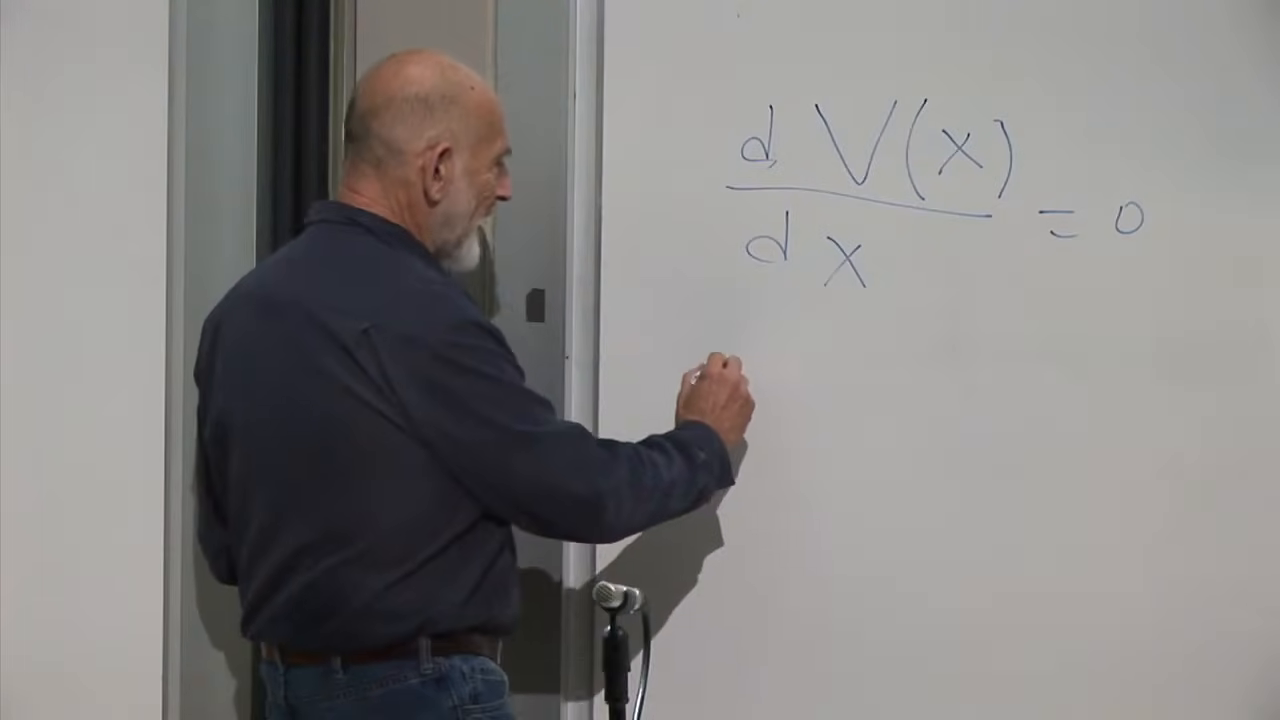
\includegraphics[width=0.74\textwidth]{lecture_03_figure_02.png}
  \caption{일차원 평형 조건: 퍼텐셜이 정지값을 갖는 곳에서 힘이 사라진다.}
  \lectureframe{00:02:51}
\end{figure}

이제 입자를 작은 양만큼 \(\delta x\)변위시켜 보자. 일차 근사에서는, \begin{equation}
  \delta V
  =V(x+\delta x)-V(x)
  =\frac{dV}{dx}\,\delta x+O(\delta x^2).
  \label{eq:first-variation-one}
\end{equation}평형 상태에서는 \(\delta x\)의 부호가 어느 쪽이든 선형항이 0이다.\begin{equation}
  \delta V=0
  \qquad\hbox{to first order.}
  \label{eq:delta-v-zero-one}
\end{equation}이는 유한하게 움직인 뒤에도 \(V\)가 정확히 변하지 않는다는 뜻이 아니다. 선도 변화가 이차 이상이라는 뜻이다. 최소와 최대 모두 이 조건을 만족한다.

\begin{figure}[htbp]
  \centering
  \begin{tikzpicture}[scale=0.95,>=Latex]
    \draw[->] (-0.2,0) -- (3.35,0) node[right] {$x$};
    \draw[->] (0,-0.2) -- (0,2.25) node[above] {$V$};
    \draw[blue!65!black,thick,smooth]
      plot coordinates {(0.2,1.85) (0.75,0.85) (1.55,0.35)
                        (2.35,0.85) (3.0,1.85)};
    \fill[red!65!black] (1.55,0.35) circle (2pt);
    \node at (1.55,-0.34) {minimum};
    \begin{scope}[xshift=4.25cm]
      \draw[->] (-0.2,0) -- (3.35,0) node[right] {$x$};
      \draw[->] (0,-0.2) -- (0,2.25) node[above] {$V$};
      \draw[blue!65!black,thick,smooth]
        plot coordinates {(0.2,0.35) (0.75,1.25) (1.55,1.85)
                          (2.35,1.25) (3.0,0.35)};
      \fill[red!65!black] (1.55,1.85) circle (2pt);
      \node at (1.55,-0.34) {maximum};
    \end{scope}
  \end{tikzpicture}
  \caption{정지 조건은 일차 미분값을 정할 뿐, 그 점이 최소인지 최대인지는 정하지 않는다.}
  \label{fig:min-max-stationary}
\end{figure}

여러 좌표 \(q_i\)에 대해서는 일차 변분이 다음과 같다.
\begin{equation}
  \delta V
  =\sum_i\frac{\partial V}{\partial q_i}\,\delta q_i.
  \label{eq:first-variation-many}
\end{equation}
이 값이 모든 독립적인 무한소 변위 \(\delta q_i\)에 대해 사라져야 한다면, 각 계수가 모두 사라져야 한다.
\begin{equation}
  \frac{\partial V}{\partial q_i}=0
  \qquad\hbox{for every }i.
  \label{eq:stationary-v-many}
\end{equation}

이차원 퍼텐셜은 롤러코스터보다는 기복이 있는 지형으로 떠올리는 편이 낫다. 정지점은 골짜기 바닥일 수도, 언덕 꼭대기일 수도, 안장점일 수도 있다. 안장점에서는 한 방향으로는 처음에 올라가고 다른 방향으로는 처음에 내려간다. 따라서 그 점에서 모든 일차 미분이 사라지더라도, 복원 거동은 한 방향에서는 안정적이고 다른 방향에서는 불안정할 수 있다.

\begin{figure}[htbp]
  \centering
  \includegraphics[width=0.76\textwidth]{lecture_03_figure_06.png}
  \caption{안장점에서는 모든 방향의 일차 변화가 사라지지만, 그 점에서 이웃한 변위는 한 축을 따라 올라가고 다른 축을 따라 내려간다.}
  \lectureframe{00:08:20}
\end{figure}

좌표가 많은 공간에서는 순수한 최대나 최소보다 안장점이 더 흔하다. 그래서 \emph{정지}라는 말이 오래도록 정확하게 쓰인다. 다음 조건은 \begin{equation}
  \delta V=0
  \label{eq:equilibrium-variation}
\end{equation}이차 거동을 미리 단정하지 않으면서 평형을 요약한다.

\section{점에서 함수로}

역학은 고립된 평형점이 아니라 운동 전체를 다룬다. 궤적은 \(x(t)\)와 같은 함수이거나, \((x(t),y(t),z(t))\)와 같은 함수들의 모음이다. 함수 전체를 변화시켜 어떤 양을 정지시키는 수학적 문제를 \emph{변분법}이라 한다. 운동에 적용하기 전에 더 간단한 예 세 가지를 살펴보자.

\subsection{최단 곡선과 측지선}

평면에 두 점을 고정하고, 두 점을 잇는 곡선을 \(y(x)\)로 나타내자. 짧은 구간에서, \begin{equation}
  ds=\sqrt{dx^2+dy^2}
  =dx\sqrt{1+\left(\frac{dy}{dx}\right)^2},
  \label{eq:line-element}
\end{equation}마지막 식은 \(dx>0\)이라고 가정한 것이다. 전체 길이는 다음 범함수로 주어진다.\begin{equation}
  S[y]=\int_{x_0}^{x_1}
  \sqrt{1+y'(x)^2}\,dx.
  \label{eq:arc-length-functional}
\end{equation}대괄호는 \(S\)가 함수 전체를 입력으로 받는다는 점을 강조한다. 양 끝점을 고정한 채 곡선을 조금씩 바꿨을 때 \begin{equation}
  \delta S=0
  \label{eq:stationary-length}
\end{equation}를 만족하는 곡선은 직선이다.

\begin{figure}[htbp]
  \centering
  \includegraphics[width=0.78\textwidth]{lecture_03_figure_07.png}
  \caption{고정된 두 끝점을 잇는 시험 곡선. 곡선의 길이는 미소 빗변 \(ds\)들을 더한 값이다.}
  \lectureframe{00:13:36}
\end{figure}

같은 문제를 곡면에서도 생각할 수 있다. 두 말뚝 사이에 줄을 팽팽히 당기면 제약된 경로 중 가장 짧은 경로를 물리적으로 떠올릴 수 있다. 길이가 정지하는 이런 곡선을 \emph{측지선}이라 한다. 평면에서는 직선이지만, 구면이나 굴곡진 표면에서는 대체로 직선이 아니다.

\subsection{페르마의 원리}

위치에 따라 속력이 달라지는 매질에서 빛은 \(c(x,y)\)공간상 최단 경로를 따르지 않을 수도 있다. 짧은 구간을 지나는 데 걸리는 시간은 거리를 그 지점의 속력으로 나눈 값이므로, \begin{equation}
  T[y]
  =\int_{x_0}^{x_1}
  \frac{\sqrt{1+y'(x)^2}}{c(x,y)}\,dx.
  \label{eq:fermat-functional}
\end{equation}페르마의 원리에 따르면 \begin{equation}
  \delta T=0.
  \label{eq:fermat-stationary}
\end{equation}이다. \(c\)가 일정하면 이 문제는 최단 거리 문제로 환원된다. 하지만 굴절률이 위치에 따라 변하는 매질에서는 최단 거리와 국소적인 전파 속력 사이의 균형으로 가장 빠른 경로가 정해진다.

\begin{figure}[htbp]
  \centering
  \includegraphics[width=0.80\textwidth]{lecture_03_figure_08.png}
  \caption{빛의 국소 속력이 위치에 따라 달라지는 매질에서 광선의 최소 시간 범함수.}
  \lectureframe{00:22:50}
\end{figure}

시사적인 농담에서는 당시 이탈리아에서 중성미자가 이례적으로 빠르게 움직였다는 최근 주장을 언급한다. 물리학적 논의는 곧 믿을 만한 예로 돌아온다. 보통의 빛은 굴절률에 따라 물질 속에서 속력이 달라진다.

\subsection{매달린 사슬}

두 점에 고정된 사슬은 현수선 형태로 놓인다. 사슬의 각 미소 부분은 중력 퍼텐셜 에너지에 기여하므로, 전체 퍼텐셜 에너지도 사슬을 따라 적분한 값이다. 여기서도 양 끝점은 고정되어 있고, 미지의 모양은 함수이며, 적분값은 정지해야 한다.

\begin{figure}[htbp]
  \centering
  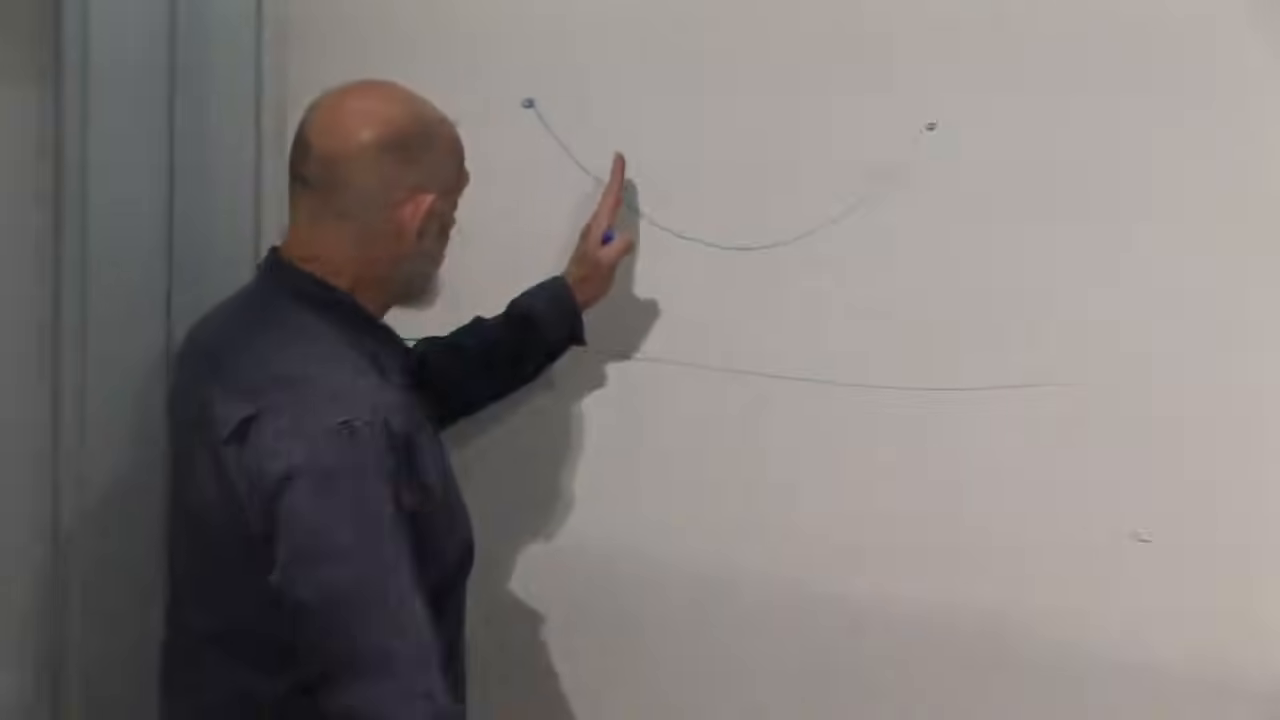
\includegraphics[width=0.76\textwidth]{lecture_03_figure_03.png}
  \caption{고정된 지지점 사이에 매달린 사슬. 정지 모양은 전체 중력 퍼텐셜 에너지로 결정된다.}
  \lectureframe{00:30:41}
\end{figure}

이 예들은 같은 구조를 갖는다. 양 끝점이 고정되어 있고, 그 사이에 함수가 있으며, 그 함수의 적분에 대한 일차 변분이 사라진다. 이처럼 전체에 주어진 조건을 미분방정식으로 바꾸는 것이 변분 문제를 푼다는 뜻이다.

\section{경계값 문제로서의 역학}

\(t\)가 독립변수이므로 궤적은 흔히 시간을 가로축으로 그린다. 그런데 물리학에는 시간을 위쪽으로 그리는 강한 관습도 있다. 한 일화에 따르면, 젊은 시절부터 노년까지의 그림을 순서대로 배열하게 하는 실험에서 글을 왼쪽에서 오른쪽으로 읽는 사람들은 그림도 왼쪽에서 오른쪽으로 배열하는 경향이 있었고, 오른쪽에서 왼쪽으로 읽는 사람들은 그 반대로, 세로쓰기에 익숙한 사람들은 세로로 배열하는 경향이 있었다. 농담의 결론은 물리학자들이야말로 시간이 위쪽으로 흐른다고 우기는 사람들이라는 것이다. 여기서는 관례에 따라 \(t\)축을 가로로 두겠다. 그러면 \(x(t)\)를 그래프로 자연스럽게 나타낼 수 있기 때문이다.

초기값 정식화에서는 \(t_0\)에서의 자료가 다음과 같다.\begin{equation}
  x(t_0)=x_0,
  \qquad
  \dot x(t_0)=v_0.
  \label{eq:initial-value-data}
\end{equation}그러면 뉴턴 방정식이 그 이후의 궤도를 결정한다. 변분 정식화는 다른 문제를 제기한다. 두 끝점 사건을 \begin{equation}
  x(t_0)=x_0,
  \qquad
  x(t_1)=x_1,
  \label{eq:boundary-value-data}
\end{equation}로 지정하고 그 사이의 물리적 경로를 구하는 것이다. 초기 속도는 더 이상 주어지지 않으며, 해의 일부로 결정된다.

\begin{figure}[htbp]
  \centering
  \includegraphics[width=0.76\textwidth]{lecture_03_figure_09.png}
  \caption{역학적 궤적 \(x(t)\). 한쪽 끝에서 위치와 기울기를 지정할 수도 있고, 두 끝점 시각에서 위치를 지정할 수도 있다.}
  \lectureframe{00:27:41}
\end{figure}

정지시킬 양은 \emph{작용}이다. \begin{equation}
  A[x]=\int_{t_0}^{t_1}L(x,\dot x,t)\,dt.
  \label{eq:action-one}
\end{equation}적분함수 \(L\)를 \emph{라그랑지안}이라 한다. 라그랑지안은 위치와 속도에 의존하며, 시간에 명시적으로 의존할 수도 있다. 작용 원리는 다음과 같다. \begin{equation}
  \delta A=0
  \label{eq:stationary-action}
\end{equation}끝점 조건 \begin{equation}
  \delta x(t_0)=\delta x(t_1)=0.
  \label{eq:fixed-endpoint-variations}
\end{equation}을 만족하는 모든 작은 경로 변분에 대해 성립한다. 끝점 조건은 필수적이다. 같은 두 사건을 잇는 이웃한 경로끼리 비교하기 때문이다.

\section{이산화에 따른 오일러--라그랑주 방정식의 유도}

작용은 경로의 무한히 많은 값에 의존하는 범함수다. 변분을 구체적으로 다루기 위해 시간 구간을 길이 \(\epsilon\)인 단계들로 나누자. \begin{equation}
  t_n=t_0+n\epsilon,
  \qquad
  x_n=x(t_n),
  \label{eq:discrete-times}
\end{equation}그리고 \(n\)번째 구간의 속도를 다음과 같이 근사한다. \begin{equation}
  v_n=\frac{x_{n+1}-x_n}{\epsilon}.
  \label{eq:discrete-velocity}
\end{equation}그러면 적분은 보통의 합으로 바뀐다. \begin{equation}
  A_\epsilon
  =\sum_{n=0}^{N-1}
  \epsilon L\left(x_n,\frac{x_{n+1}-x_n}{\epsilon}\right).
  \label{eq:discrete-action}
\end{equation}\(n\)는 시간 구간의 첨자이고, 뒤에서 공간 좌표와 입자를 나타내는 \(i\)를 쓸 수 있도록 이 표기를 택했다.

\begin{figure}[htbp]
  \centering
  \includegraphics[width=0.82\textwidth]{lecture_03_figure_10.png}
  \caption{시간 구간들로 대체한 궤적. 내부의 한 점을 변분하면 그 양옆 구간만 바뀐다.}
  \lectureframe{00:38:30}
\end{figure}

다른 모든 \(x_k\)를 고정한 채 내부의 한 점 \(x_n\)만 변분하자. 합에서 \(x_n\)에 의존하는 항은 두 개뿐이다. \begin{align}
  A_\epsilon\big|_{x_n}
  &=
  \epsilon L\left(x_n,\frac{x_{n+1}-x_n}{\epsilon}\right)
  \notag\\
  &\quad+
  \epsilon L\left(x_{n-1},
                  \frac{x_n-x_{n-1}}{\epsilon}\right).
  \label{eq:two-neighbor-terms}
\end{align}미분하면 다음을 얻는다. \begin{align}
  0=\frac{\partial A_\epsilon}{\partial x_n}
  &=
  \epsilon\frac{\partial L_n}{\partial x_n}
  -\frac{\partial L_n}{\partial v_n}
  +\frac{\partial L_{n-1}}{\partial v_{n-1}}.
  \label{eq:discrete-el-variation}
\end{align}부호가 반대인 데에는 간단한 기하학적 이유가 있다. \(x_n\)를 높이면 뒤쪽 구간의 기울기는 커지고 앞쪽 구간의 기울기는 작아진다.

\begin{figure}[htbp]
  \centering
  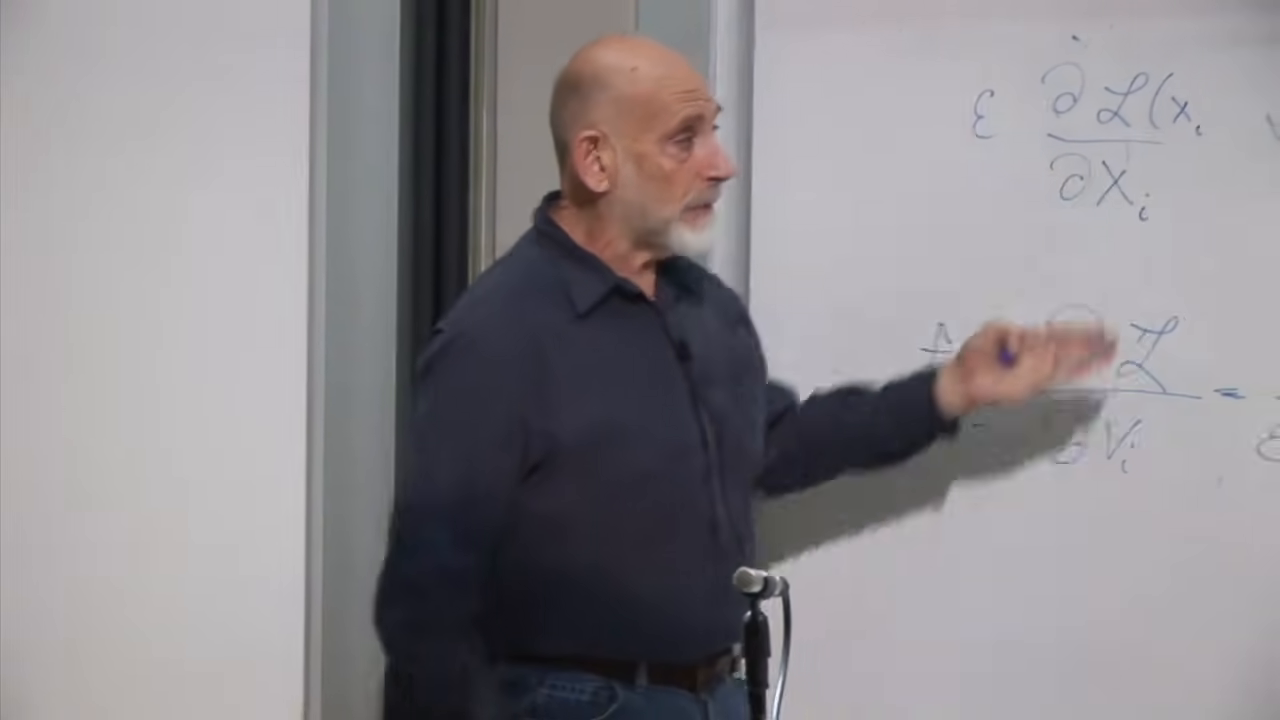
\includegraphics[width=0.74\textwidth]{lecture_03_figure_04.png}
  \caption{위치에 대한 직접 미분항과 양옆 구간의 속도 미분에서 오는 두 기여.}
  \lectureframe{00:45:26}
\end{figure}

식~\eqref{eq:discrete-el-variation}을 정리하면 다음과 같다. \begin{equation}
  \frac{1}{\epsilon}
  \left(
    \frac{\partial L_n}{\partial v_n}
    -\frac{\partial L_{n-1}}{\partial v_{n-1}}
  \right)
  =
  \frac{\partial L_n}{\partial x_n}.
  \label{eq:discrete-el}
\end{equation}왼쪽은 이웃한 두 값의 차분몫이다. \(\epsilon\to0\)가 되면 꺾은선은 매끄러운 경로가 되고, 차분몫은 시간 미분으로 바뀐다. \begin{equation}
  \boxed{
  \frac{d}{dt}\left(\frac{\partial L}{\partial\dot x}\right)
  =
  \frac{\partial L}{\partial x}}
  .
  \label{eq:euler-lagrange-one}
\end{equation}이것이 오일러--라그랑주 방정식이다.

\begin{figure}[htbp]
  \centering
  \includegraphics[width=0.78\textwidth]{lecture_03_figure_11.png}
  \caption{모든 내부 시간 구간에서 정지 조건을 적용해 얻은 완성된 오일러--라그랑주 방정식.}
  \lectureframe{00:49:25}
\end{figure}

\(L\)가 주어지면 식~\eqref{eq:euler-lagrange-one}은 일종의 기계처럼 작동한다. 주어진 함수를 미분하면 경로에 대한 미분방정식이 나온다.

\begin{classroomqa}\audiencequestion{오일러--라그랑주 결과는 \(x\)와 \(\dot x\)의 임의의 함수에 대해 성립하나요?\lecturetimestamp{00:49:37--00:50:24}}\lecturerresponse{미분에 필요한 정칙성 조건이 충족되면 성립합니다. 독립변수 \(x\)가 \(t\)의 역할을 하고 미지 함수 \(y(x)\)가 \(x(t)\)의 역할을 하도록 바꾸어 쓰면, 호의 길이 예제도 정확히 같은 형식입니다. 그 경우 오일러--라그랑주 방정식의 해는 직선입니다.}\end{classroomqa}

\section{라그랑지안으로부터 뉴턴 방정식 유도하기}

퍼텐셜 \(V(x)\) 속에서 직선 운동하는 입자에 대해 다음을 택하자. \begin{equation}
  L(x,\dot x)=T-V
  =\frac12m\dot x^2-V(x).
  \label{eq:lagrangian-tv-one}
\end{equation}전체 에너지가 \(T+V\)이므로 마이너스 부호가 이상해 보일 수 있다. 하지만 라그랑지안은 에너지가 아니다. 오일러--라그랑주 방정식이 올바른 운동을 내놓는지가 판별 기준이다. 부호를 두고 모의 투표를 하자는 제안은 받아들이지 않는다. 답은 투표로 정하는 것이 아니라 확인해야 한다.

먼저, \begin{equation}
  \frac{\partial L}{\partial\dot x}=m\dot x.
  \label{eq:conjugate-momentum-one}
\end{equation}이것은 운동량이다. 더 일반적으로 좌표 \(q\)에 켤레인 운동량은 다음과 같이 정의한다. \begin{equation}
  p_q=\frac{\partial L}{\partial\dot q}.
  \label{eq:conjugate-momentum-general}
\end{equation}식~\eqref{eq:conjugate-momentum-one}을 시간에 대해 미분하면 \(m\ddot x\)을 얻고, \begin{equation}
  \frac{\partial L}{\partial x}
  =-\frac{dV}{dx}.
  \label{eq:lagrangian-position-derivative}
\end{equation}가 성립한다. 따라서 오일러--라그랑주 방정식은 \begin{equation}
  m\ddot x=-\frac{dV}{dx}=F(x),
  \label{eq:newton-from-action}
\end{equation}이 되며, 이것이 뉴턴의 제이 법칙이다.

\begin{figure}[htbp]
  \centering
  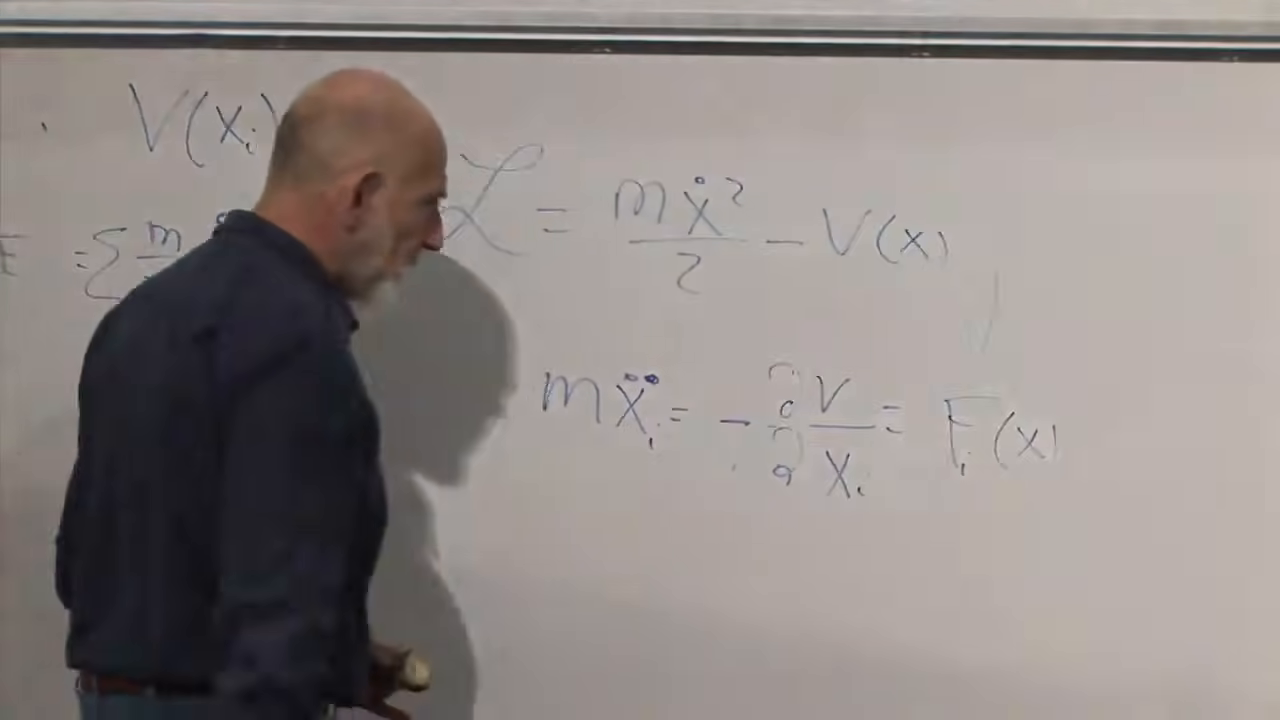
\includegraphics[width=0.80\textwidth]{lecture_03_figure_05.png}
  \caption{운동 에너지, 퍼텐셜 에너지, \(L=T-V\), 그리고 되찾은 뉴턴 방정식의 성분별 표현을 한 판에 나타냈다.}
  \lectureframe{00:57:52}
\end{figure}

좌표가 여러 개 \(q_i\)이면, \begin{equation}
  L(\mathbf q,\dot{\mathbf q})
  =\sum_i\frac12m_i\dot q_i^{\,2}-V(q_1,q_2,\ldots),
  \label{eq:lagrangian-tv-many}
\end{equation}좌표마다 방정식이 하나씩 있다. \begin{equation}
  \frac{d}{dt}\left(\frac{\partial L}{\partial\dot q_i}\right)
  =\frac{\partial L}{\partial q_i}
  \quad\Longrightarrow\quad
  m_i\ddot q_i=-\frac{\partial V}{\partial q_i}=F_i.
  \label{eq:euler-lagrange-many}
\end{equation}궤적은 여전히 하나의 곡선이지만, 이제 고차원 배치 공간을 지난다.

\begin{classroomqa}\audiencequestion{뉴턴 법칙에서 역으로 출발해 답을 재현하는 범함수를 고안한 것뿐인가요?\lecturetimestamp{00:58:07--01:00:04}}\lecturerresponse{그렇게 보는 것은 생산적인 관점이 아닙니다. 라그랑지안은 물리계를 간결하게 규정합니다. 모든 좌표와 속도를 포함하는 하나의 함수에 운동 방정식 전체를 담습니다. 새로운 이론에서는 물리학자들이 각 방정식을 따로 추측하기보다 보통 작용을 제안하고 방정식을 유도합니다.}\end{classroomqa}

이런 통합은 한 가지 장점이다. 좌표 선택의 자유도 또 다른 장점이다. 직선이 최단이라는 명제는 평면을 데카르트 좌표, 극좌표 또는 곡선 좌표 중 무엇으로 기술하는지에 좌우되지 않는다. 마찬가지로 작용의 정지 조건도 좌표에 무관하지만, \(L\)의 식과 그에 따른 성분 방정식은 좌표에 따라 달라진다.

\section{회전목마에서 본 자유 입자}

\((x,y)\)를 관성계의 데카르트 좌표, \((X,Y)\)를 각속도 \(\omega\)로 균일하게 회전하는 좌표라고 하자. 여기서 사용한 방향 규약에 따르면, \begin{align}
  x&=X\cos\omega t+Y\sin\omega t,
  \notag\\
  y&=-X\sin\omega t+Y\cos\omega t.
  \label{eq:rotating-coordinate-map}
\end{align}두 좌표계 사이의 각도는 \(\omega t\)이다.

\begin{figure}[htbp]
  \centering
  \includegraphics[width=0.76\textwidth]{lecture_03_figure_12.png}
  \caption{관성계의 데카르트 좌표축과 균일 회전하는 좌표축. 같은 점도 회전 좌표계에서는 시간에 따라 변하는 좌표를 갖는다.}
  \lectureframe{01:06:05}
\end{figure}

자유 입자의 관성계 라그랑지안은 다음과 같다. \begin{equation}
  L_{\mathrm{in}}
  =\frac{m}{2}\left(\dot x^2+\dot y^2\right).
  \label{eq:free-inertial-lagrangian}
\end{equation}식~\eqref{eq:rotating-coordinate-map}을 미분하고 \(\sin^2\omega t+\cos^2\omega t=1\)를 이용하자. 삼각함수 항들을 합하면 \begin{align}
  \dot x^2+\dot y^2
  &=
  \dot X^2+\dot Y^2\\
  &\quad+\omega^2(X^2+Y^2)\\
  &\quad+2\omega(Y\dot X-X\dot Y).
  \label{eq:rotating-speed}
\end{align}가 된다. 따라서 \begin{align}
  L_{\mathrm{rot}}
  &=
  \frac{m}{2}(\dot X^2+\dot Y^2)\\
  &\quad+\frac{m\omega^2}{2}(X^2+Y^2)\\
  &\quad+m\omega(Y\dot X-X\dot Y).
  \label{eq:rotating-lagrangian}
\end{align}이다.

\begin{figure}[htbp]
  \centering
  \includegraphics[width=0.84\textwidth]{lecture_03_figure_13.png}
  \caption{변환된 자유 입자 라그랑지안: 보통의 운동 에너지, 이차 원심력 항, 속도에 선형인 항.}
  \lectureframe{01:12:16}
\end{figure}

좌표에 대한 이차항은 \(-V_{\mathrm{fict}}\)의 형태이며, 여기서 \begin{equation}
  V_{\mathrm{fict}}
  =-\frac{m\omega^2}{2}(X^2+Y^2).
  \label{eq:centrifugal-potential}
\end{equation}이다. 이 항은 바깥쪽으로 갈수록 작아지므로 원심력 \(m\omega^2(X,Y)\)을 만들어 낸다.

식~\eqref{eq:rotating-lagrangian}의 마지막 항은 좌표와 속도 모두에 선형이다. 오일러--라그랑주 방정식을 적용하면 \begin{align}
  m\ddot X&=m\omega^2X-2m\omega\dot Y,
  \notag\\
  m\ddot Y&=m\omega^2Y+2m\omega\dot X.
  \label{eq:rotating-equations}
\end{align}를 얻는다. \(\omega^2\)에 비례하는 항은 원심력에 해당하고, 속도에 비례하는 항은 코리올리 힘에 해당한다. 회전 평면 안에서 벡터로 쓰면 \begin{equation}
  \mathbf F_{\mathrm{C}}
  =-2m\,\boldsymbol\omega\times\mathbf v_{\mathrm{rot}},
  \label{eq:coriolis-vector}
\end{equation}이며, 반대 방향 규약을 택하면 부호를 조정해야 한다.

\begin{figure}[htbp]
  \centering
  \includegraphics[width=0.84\textwidth]{lecture_03_figure_14.png}
  \caption{회전 좌표계의 방정식. 좌표에 비례하는 항은 원심 가속도를, 속도 성분 간 교차항은 코리올리 가속도를 만든다.}
  \lectureframe{01:20:20}
\end{figure}

핵심은 대수 계산이 사라진다는 것이 아니다. 하나의 스칼라 함수에 좌표 변환을 적용하면 서로 결합된 두 방정식과 두 가상력이 모두 나온다는 점이다.

\begin{classroomqa}\audiencequestion{이 방법은 곡선 좌표가 아무리 복잡해도 쓸 수 있나요?\lecturetimestamp{01:22:01--01:22:17}}\lecturerresponse{그렇습니다. 새 좌표는 곡선 좌표여도 되고, 회전 좌표처럼 시간에 명시적으로 의존해도 됩니다. 작용을 새 변수로 다시 쓴 다음 같은 오일러--라그랑주 규칙을 적용하면 됩니다.}\end{classroomqa}

\section{극좌표와 순환 각도}

보통의 극좌표에서는, \begin{equation}
  x=r\cos\theta,
  \qquad
  y=r\sin\theta.
  \label{eq:polar-map}
\end{equation}\(r\)와 \(\theta\)는 모두 시간에 따라 변할 수 있다. 미분한 다음 제곱을 더하면 \begin{equation}
  \dot x^2+\dot y^2
  =\dot r^2+r^2\dot\theta^2.
  \label{eq:polar-speed}
\end{equation}를 얻는다. 중심 퍼텐셜 \(V(r)\)에 대해서는, \begin{equation}
  L
  =\frac{m}{2}\left(\dot r^2+r^2\dot\theta^2\right)-V(r).
  \label{eq:polar-lagrangian}
\end{equation}이다.

\begin{figure}[htbp]
  \centering
  \includegraphics[width=0.80\textwidth]{lecture_03_figure_15.png}
  \caption{극좌표의 기하학과 운동 에너지를 방사 운동 및 각운동으로 분해한 모습.}
  \lectureframe{01:23:30}
\end{figure}

방사 방향 방정식은 다음과 같다. \begin{equation}
  m\ddot r
  =mr\dot\theta^2-\frac{dV}{dr}.
  \label{eq:radial-equation}
\end{equation}첫 번째 항은 입자 자체의 각운동과 관련된 바깥쪽 원심력 기여다.

각도에 대해서는, \begin{equation}
  \frac{d}{dt}\left(\frac{\partial L}{\partial\dot\theta}\right)
  =\frac{\partial L}{\partial\theta}=0,
  \label{eq:theta-el}
\end{equation}중심 퍼텐셜이 \(\theta\)에 명시적으로 의존하지 않기 때문이다. 따라서 \begin{equation}
  \frac{d}{dt}\left(mr^2\dot\theta\right)=0,
  \qquad
  mr^2\dot\theta=\ell,
  \label{eq:angular-momentum}
\end{equation}이며, \(\ell\)는 보존되는 각운동량이다.

\begin{figure}[htbp]
  \centering
  \includegraphics[width=0.82\textwidth]{lecture_03_figure_16.png}
  \caption{각도에 대한 오일러--라그랑주 방정식의 우변은 0이며, 이에 따라 \(mr^2\dot\theta\)의 보존이 드러난다.}
  \lectureframe{01:29:25}
\end{figure}

각도 방정식에서 \begin{equation}
  \dot\theta=\frac{\ell}{mr^2}.
  \label{eq:theta-dot-angular-momentum}
\end{equation}를 얻는다. 이를 식~\eqref{eq:radial-equation}에 대입하면 \(r\)에 대한 방정식 하나만 남는다. \begin{equation}
  m\ddot r
  =\frac{\ell^2}{mr^3}-\frac{dV}{dr}.
  \label{eq:effective-radial-equation}
\end{equation}

\(L\)에서 빠져 있는 좌표를, 그 좌표가 각도가 아니더라도 관례적으로 \emph{순환} 좌표라고 부른다. \(q\)가 순환 좌표이면 \begin{equation}
  \frac{\partial L}{\partial q}=0
  \quad\Longrightarrow\quad
  \frac{d}{dt}\left(\frac{\partial L}{\partial\dot q}\right)=0.
  \label{eq:cyclic-conservation}
\end{equation}이다. 그 켤레 운동량은 보존된다. 이는 대칭성과 보존 법칙 사이의 일반적인 연결을 엿보게 해 준다.

\section{의미, 에너지, 적용 범위에 관한 질문}

이어지는 질문들은 이 형식론의 더 깊은 내용이 어디에 있는지 드러낸다.

\begin{classroomqa}\audiencequestion{라그랑지안이 올바른 고전 방정식을 준다는 사실을 발견하는 것 외에, 라그랑지안을 도출할 독립적인 근거가 있나요?\lecturetimestamp{01:33:25--01:35:07}}\lecturerresponse{역사적으로 한 세기가 넘는 고전역학의 발전을 통해 입자와 파동, 전자기장이 모두 이 형식으로 나타날 수 있음이 밝혀졌습니다. 고전적인 수준에서 이처럼 축적된 성공은 자연 법칙이 구성되는 방식에 관한 경험적 사실입니다. 더 깊은 설명은 양자역학에서 나오며, 그 논의는 뒤로 미루겠습니다.}\end{classroomqa}

\begin{classroomqa}\audiencequestion{회전 좌표계 라그랑지안에서 속도에 선형인 항에 보통의 운동 에너지나 퍼텐셜 에너지라는 해석을 붙일 수 있나요?\lecturetimestamp{01:35:08--01:36:23}}\lecturerresponse{아니요. 시간 병진에 대응하는 보존량은 해밀토니안 구성으로 구합니다. \(L\)의 모든 항을 운동 에너지나 퍼텐셜 에너지로 읽어 내는 것이 아닙니다. 식~\eqref{eq:rotating-lagrangian}에서는 속도에 선형인 항이 \(\sum_a\dot q_a\,\partial L/\partial\dot q_a-L\)에서 상쇄됩니다. 해밀토니안 형식에서는 이를 체계적으로 다룰 것입니다.}\end{classroomqa}

실제로 \(L_{\mathrm{rot}}\)는 시간에 명시적으로 의존하지 않으므로 \begin{equation}
  \begin{aligned}
    H_{\mathrm{rot}}
    &=\dot X\frac{\partial L}{\partial\dot X}
     +\dot Y\frac{\partial L}{\partial\dot Y}-L\\
    &=\frac{m}{2}(\dot X^2+\dot Y^2)
     -\frac{m\omega^2}{2}(X^2+Y^2)
  \end{aligned}
  \label{eq:rotating-hamiltonian-preview}
\end{equation}가 보존된다. 이것은 회전 좌표계의 자코비 적분이며, 관성계 관찰자가 부여하는 에너지와 수치상 같은 양은 아니다. 시간 의존적인 좌표 변환을 거치면 에너지의 수치적 형태가 보존되지 않을 수 있다.

\begin{classroomqa}\audiencequestion{중력 때문에 궤적이 휘어진다면 어떻게 하나요?\lecturetimestamp{01:36:30--01:37:10}}\lecturerresponse{뉴턴 중력이라면 중심력 라그랑지안에 \(V(r)=-GMm/r\)를 쓰면 됩니다. 휘어진 시공간은 일반상대론에 속하며 여기서는 전제하지 않습니다.}\end{classroomqa}

\begin{classroomqa}\audiencequestion{원심 퍼텐셜과 그 에너지는 그저 가상적인 것인가요?\lecturetimestamp{01:37:13--01:40:14}}\lecturerresponse{회전하는 플랫폼의 관찰자는 유효 힘을 측정하며 회전 좌표계의 보존량을 일관되게 사용할 수 있습니다. \emph{가상적}이라는 말은 이 항들이 비관성계 기술에서 생겨난다는 뜻이지, 관찰되는 효과가 허상이라는 뜻이 아닙니다. 에너지 자체는 일반적인 시간 의존 좌표 변환에서 불변량이 아닙니다.}\end{classroomqa}

\begin{classroomqa}\audiencequestion{속도에 의존하는 코리올리 힘은 어느 방향을 향하나요?\lecturetimestamp{01:40:22--01:42:36}}\lecturerresponse{회전 좌표계에서의 속도에 수직이며, 크기는 속력과 좌표계의 각속도에 비례합니다. 평면에서는 식\(\dot X\)과 \(\dot Y\)가 서로 반대 부호로 바뀌며, 식~\eqref{eq:rotating-equations}과 같습니다.}\end{classroomqa}

\begin{figure}[htbp]
  \centering
  \includegraphics[width=0.76\textwidth]{lecture_03_figure_17.png}
  \caption{속도 성분 간 교차항의 형태: 코리올리 힘은 회전 좌표계에서의 속도에 수직이다.}
  \lectureframe{01:41:40}
\end{figure}

\begin{classroomqa}\audiencequestion{출발점이 되는 라그랑지안은 반드시 관성계에서 써야 하나요?\lecturetimestamp{01:42:37--01:44:00}}\lecturerresponse{보통의 자유 입자에서는 뉴턴의 관성계 법칙이 간단한 출발 형태 \(m(\dot x^2+\dot y^2)/2\)를 줍니다. 이 물리 법칙을 알고 있다면 작용을 다른 어떤 좌표로도 변환할 수 있습니다. 회전 좌표계에서도 똑같이 간단한 운동 에너지 식을 쓸 수 있다고 독립적으로 가정해서는 안 됩니다.}\end{classroomqa}

자기장 속 하전 입자에서도 같은 종류의 속도 선형 항이 나타난다. \begin{equation}
  L_{\mathrm{em}}
  =\frac12m\mathbf v^2
   +q\mathbf A(\mathbf r,t)\cdot\mathbf v
   -q\phi(\mathbf r,t).
  \label{eq:electromagnetic-lagrangian}
\end{equation}평면에 수직인 균일 자기장에 대해 대칭 게이지 \(\mathbf A=\tfrac12\mathbf B\times\mathbf r\)를 택하면, 코리올리 항과 대수적 구조가 같은 \(X\dot Y-Y\dot X\)에 비례하는 항이 생긴다.

\begin{figure}[htbp]
  \centering
  \includegraphics[width=0.82\textwidth]{lecture_03_figure_18.png}
  \caption{균일 자기장 속 하전 입자와의 비교를 이끌어 내는, 회전 좌표계 라그랑지안의 속도 선형 항.}
  \lectureframe{01:44:40}
\end{figure}

\begin{classroomqa}\audiencequestion{매끄럽다는 조건 외에 라그랑지안이 될 수 있는 함수에 제약이 있나요?\lecturetimestamp{01:44:46--01:45:06}}\lecturerresponse{있습니다. 다만 관련 제약을 다루려면 아직 설명하지 않은 더 많은 구조가 필요하므로 뒤로 미룹니다. 여기서의 핵심은 제안된 라그랑지안이 어떻게 방정식과 보존 법칙을 만들어 내는지입니다.}\end{classroomqa}

회전 좌표계 방정식은 원운동도 허용한다. 관성계에 고정된 점은 회전목마에서 보면 회전하는 원점을 중심으로 돈다. 자기장과의 유사성은 하전 입자가 원운동인 사이클로트론 운동을 할 수 있는 이유도 설명한다.

\begin{classroomqa}\audiencequestion{하전 입자는 그 원을 계속 돌까요, 아니면 복사 때문에 궤도가 붕괴할까요?\lecturetimestamp{01:46:11--01:47:21}}\lecturerresponse{논의 중인 입자만의 방정식에는 복사가 포함되어 있지 않습니다. 전자기장과의 결합 및 복사 반작용까지 포함하면 가속하는 고전적 전하는 복사할 수 있습니다. 따라서 복사는 절단된 방정식에서 나타나는 궤도와 모순되는 것이 아니라 별도의 물리적 효과입니다.}\end{classroomqa}

\begin{classroomqa}\audiencequestion{허리케인은 이 논의와 어떤 관련이 있나요?\lecturetimestamp{01:47:30--01:47:50}}\lecturerresponse{대규모 대기 운동은 자전하는 지구 위에서 일어나므로 코리올리 효과가 중요합니다. 이를 제대로 유도하는 일은 기상학에 속하며 여기서는 다루지 않습니다.}\end{classroomqa}

\begin{classroomqa}\audiencequestion{작용 형식은 모든 물리 법칙을 포괄한다고 보나요? 진정한 예외가 있다면 무엇을 뜻할까요?\lecturetimestamp{01:47:57--01:49:01}}\lecturerresponse{논의 범위에 속하는 것으로 알려진 모든 닫힌 기본 이론은 작용으로 정리할 수 있습니다. 뉴턴 입자, 맥스웰 장, 일반상대론, 표준 모형이 여기에 포함됩니다. 점성 항력처럼 보이는 반례는 환경의 자유도를 생략했을 때 생깁니다. 유체나 미시적 열욕조까지 포함하도록 계를 확장하면 기본 기술은 다시 이 형식에 들어맞습니다. 따라서 근본적인 수준의 진정한 예외가 발견된다면 대단히 중요한 발견일 것입니다.}\end{classroomqa}\chapter{대칭성과 보존 법칙}

\lectureoverview{정지 작용과 오일러--라그랑주 방정식은 고전역학의 핵심 절반이고, 해밀턴 형식은 나머지 절반이다. 여기서는 첫 번째 절반을 충분히 전개하여 하나의 심오한 규칙을 드러내겠다. 라그랑지안의 모든 연속 대칭은 보존량을 만들어 낸다. 병진과 회전에서 이 규칙을 찾아보고, 일반적인 무한소 변환에 대해 증명한 다음, 이 논증이 적용되는 경우와 적용되지 않는 경우를 자세히 살펴보겠다.}

\section{물리를 설명하는 데 필요한 최소한의 수학}

칠판에 이미 적힌 식들은 슈뢰딩거 방정식과 조금 닮아 보일지 모르지만, 오늘 다룰 주제는 그것이 아니다. 주제는 대칭성과 보존이다. 방정식 없이 이 둘의 관계를 제대로 설명할 방법은 없다. 방정식 자체는 기초적이다. 중요한 것은 구조가 눈에 드러나도록 식들을 배열하는 일이다. 결과의 이름은 Scientific American에서 따올지 모르지만, 여기서는 물리학자가 유도하듯 그 결과를 이끌어 내는 데 필요한 최소한의 수학을 다루고자 한다.

작은 매개변수 \(\epsilon\)를 도입하자. \(\epsilon\)에 비례하는 항은 남기고 \(O(\epsilon^2)\)은 버린다. 이는 극한 논증을 줄여 쓴 것이지, 영이 아닌 실수의 제곱이 문자 그대로 영이라는 주장은 아니다. 보통 함수 \(f(x,y)\)에 대해서는
\begin{equation}
  \delta f
  =\frac{\partial f}{\partial x}\,\delta x
   +\frac{\partial f}{\partial y}\,\delta y
   +O(\epsilon^2),
  \label{eq:first-variation-f}
\end{equation}
여기서 \(\delta x\)와 \(\delta y\)는 모두 \(\epsilon\)에 비례한다. 기호 \(\delta f\)는 \(f\)의 변화를 뜻하며, \(\delta\)라는 수와 \(f\)의 곱을 뜻하지 않는다. 정지점에서는 다음을 만족한다.
\begin{equation}
  \delta f=0
  \qquad\hbox{to first order.}
  \label{eq:stationary-f}
\end{equation}

역학적 경로 \(q_i(t)\)에 대응하는 양은 작용이다.
\begin{equation}
  S[q]=\int_{t_1}^{t_2}L(q,\dot q,t)\,dt.
  \label{eq:action-l4}
\end{equation}
양 끝점을 고정한 채 경로를 변분하면
\begin{equation}
  \delta S
  =\int_{t_1}^{t_2}dt\,
   \sum_i\left(
     \frac{\partial L}{\partial q_i}\,\delta q_i
     +\frac{\partial L}{\partial\dot q_i}\,\delta\dot q_i
   \right).
  \label{eq:action-variation-l4}
\end{equation}
두 항이 나타나는 이유는 경로를 바꾸면 위치와 속도가 모두 바뀌기 때문이다. 부분적분과
\(\delta q_i(t_1)=\delta q_i(t_2)=0\)를 함께 이용하면 \(\delta S=0\)는 다음과 같이 된다.
\begin{equation}
  \frac{d}{dt}\left(\frac{\partial L}{\partial\dot q_i}\right)
  -\frac{\partial L}{\partial q_i}=0.
  \label{eq:el-l4}
\end{equation}

\begin{figure}[htbp]
  \centering
  \includegraphics[width=0.76\textwidth]{lecture_04_figure_05.png}
  \caption{대칭성과 보존을 논의할 출발점으로 다시 살펴보는 오일러--라그랑주 방정식.}
  \lectureframe{00:09:00}
\end{figure}

정확한 표현은 \emph{정지 작용}이지, 반드시 최소 작용인 것은 아니다. 이 차이는 끝부분에서 다시 다루겠다.

\section{일반화 좌표와 켤레 운동량}

일반적인 역학을 표현하기에는 데카르트 좌표만으로는 부족하다. 좌표는 입자의 위치, 각도, 집단 변수 또는 장의 진폭일 수 있으므로 이를 \(q_i\)라 부른다. 라그랑지안은 동역학을 압축해 기술한다. 표준 모형을 아주 압축된 표기 없이 전부 적으면 대략 한 페이지를 차지한다. 장의 각 성분마다 운동 방정식을 따로 적는다면 훨씬 더 많은 지면이 필요할 것이다. 하나의 함수 \(L\)가 그 모든 내용을 담는다.

\(q_i\)에 켤레인 운동량은
\begin{equation}
  p_i=\frac{\partial L}{\partial\dot q_i}.
  \label{eq:canonical-momentum-l4}
\end{equation}
이 때문에 일반화 좌표를 전통적으로 \(q\)라 부르고, 이에 대응하는 운동량은 \(p\)라 부른다. 따라서 \(p\)와 \(q\)를 얻게 된다. 이 표기법으로 식 ~\eqref{eq:el-l4}는 다음과 같다.
\begin{equation}
  \dot p_i=\frac{\partial L}{\partial q_i}.
  \label{eq:momentum-el-l4}
\end{equation}

익숙한 1차원 입자의 경우,
\begin{equation}
  L=\frac{m\dot x^2}{2}-V(x),
  \qquad
  \frac{\partial L}{\partial\dot x}=m\dot x,
  \label{eq:particle-momentum-l4}
\end{equation}
따라서 켤레 운동량은 보통의 운동량이다.

\begin{figure}[htbp]
  \centering
  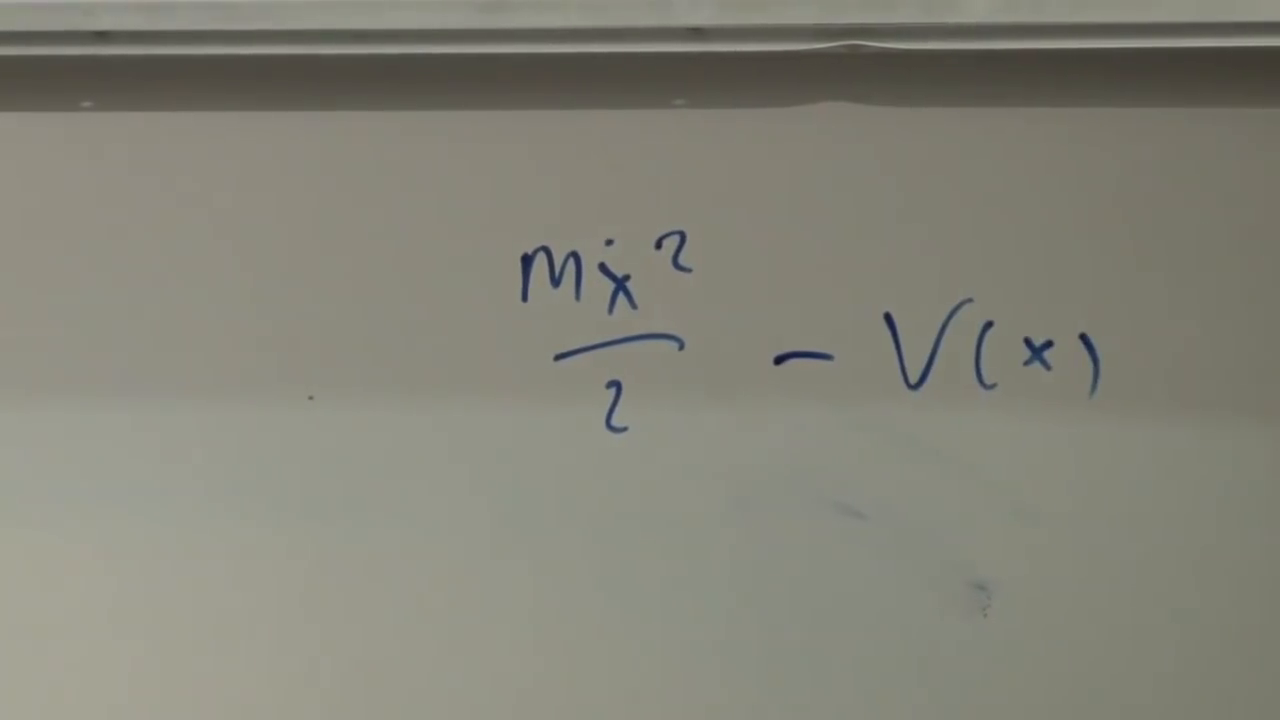
\includegraphics[width=0.72\textwidth]{lecture_04_figure_02.png}
  \caption{켤레 운동량을 \(m\dot x\)와 동일시할 때 사용하는 운동에너지에서 퍼텐셜 에너지를 뺀 라그랑지안.}
  \lectureframe{00:14:48}
\end{figure}

\(q_i\)가 \(L\)에 나타나지 않으면 \(\dot p_i=0\)이다. 이는 보존 법칙을 얻는 익숙한 순환좌표 방법이다. 실제 관계는 더 일반적이며, 이를 증명하기에 앞서 예시를 통해 알아보면 유익하다.

\section{설명에 앞서 살펴보는 보존 법칙}

\subsection{두 좌표와 두 좌표의 차이에만 의존하는 퍼텐셜}

두 질량을 모두 1로 두고 다음과 같이 하자.
\begin{equation}
  L=\frac{\dot q_1^{\,2}+\dot q_2^{\,2}}{2}-V(q_1-q_2).
  \label{eq:separation-lagrangian}
\end{equation}
두 입자가 직선 위에 있다고 생각해도 좋다. 두 입자의 상호작용은 서로의 간격에만 의존한다.

\begin{figure}[htbp]
  \centering
  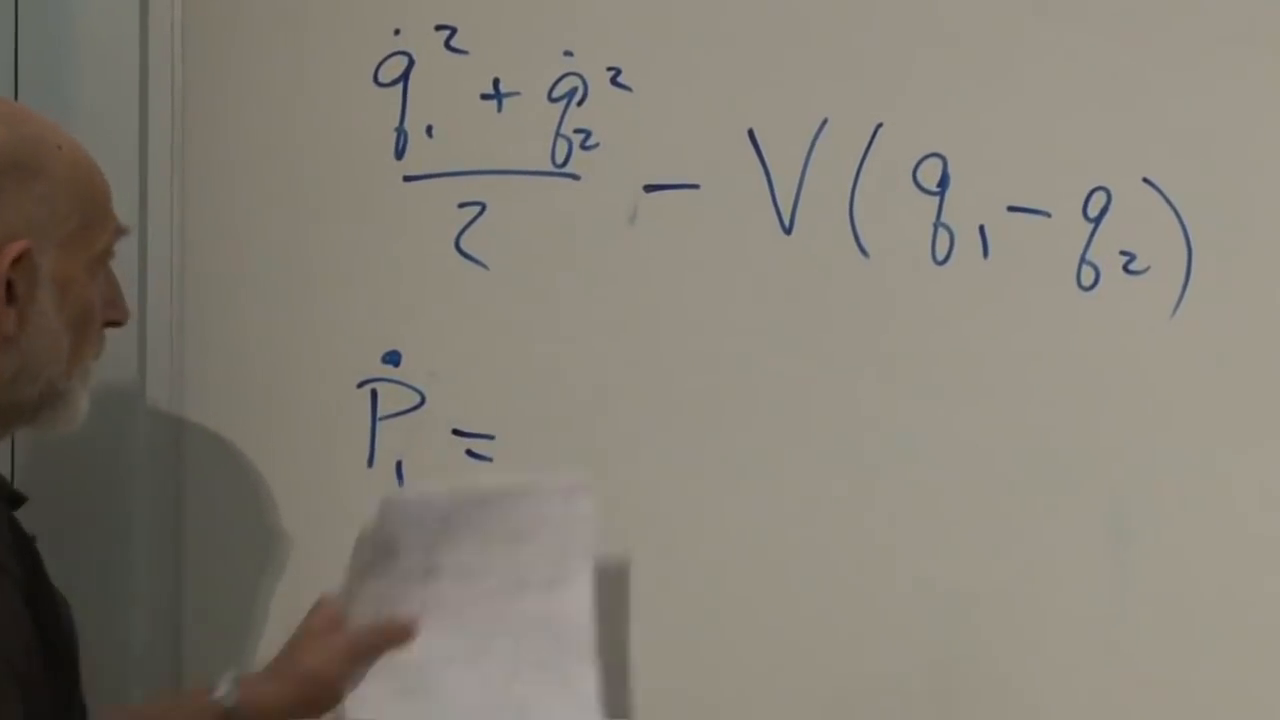
\includegraphics[width=0.78\textwidth]{lecture_04_figure_03.png}
  \caption{두 좌표에 대한 라그랑지안과 첫 번째 운동량 방정식의 시작 부분.}
  \lectureframe{00:18:56}
\end{figure}

\(V\)의 인수에 대한 미분을 \(V'\)로 쓰면,
\begin{align}
  \dot p_1&=-V'(q_1-q_2),
  \notag\\
  \dot p_2&=+V'(q_1-q_2).
  \label{eq:separation-momentum-equations}
\end{align}
\(q_2\)를 증가시키면 \(q_1-q_2\)가 감소하므로 두 번째 식의 부호는 반대가 된다.

\begin{classroomqa}
  \audiencequestion{첫 번째 운동량 방정식에 \(V'\)가 들어가야 하나요? 마이너스 부호는 어디서 나오나요?
  \lecturetimestamp{00:20:52--00:21:35}}
  \lecturerresponse{오일러--라그랑주 방정식은 라그랑지안이 0이라는 뜻이 아니라
  \(\dot p_1=\partial L/\partial q_1\)라고 말합니다.
  \(L=T-V\)이므로 \(q_1\)에 대해 미분하면
  \(-V'\)가 됩니다. \(q_2\)에 대해 미분하면 \(q_1-q_2\)에서 마이너스 부호가 하나 더 생기므로, 두 번째 방정식에는 \(+V'\)가 들어갑니다.}
\end{classroomqa}

\begin{figure}[htbp]
  \centering
  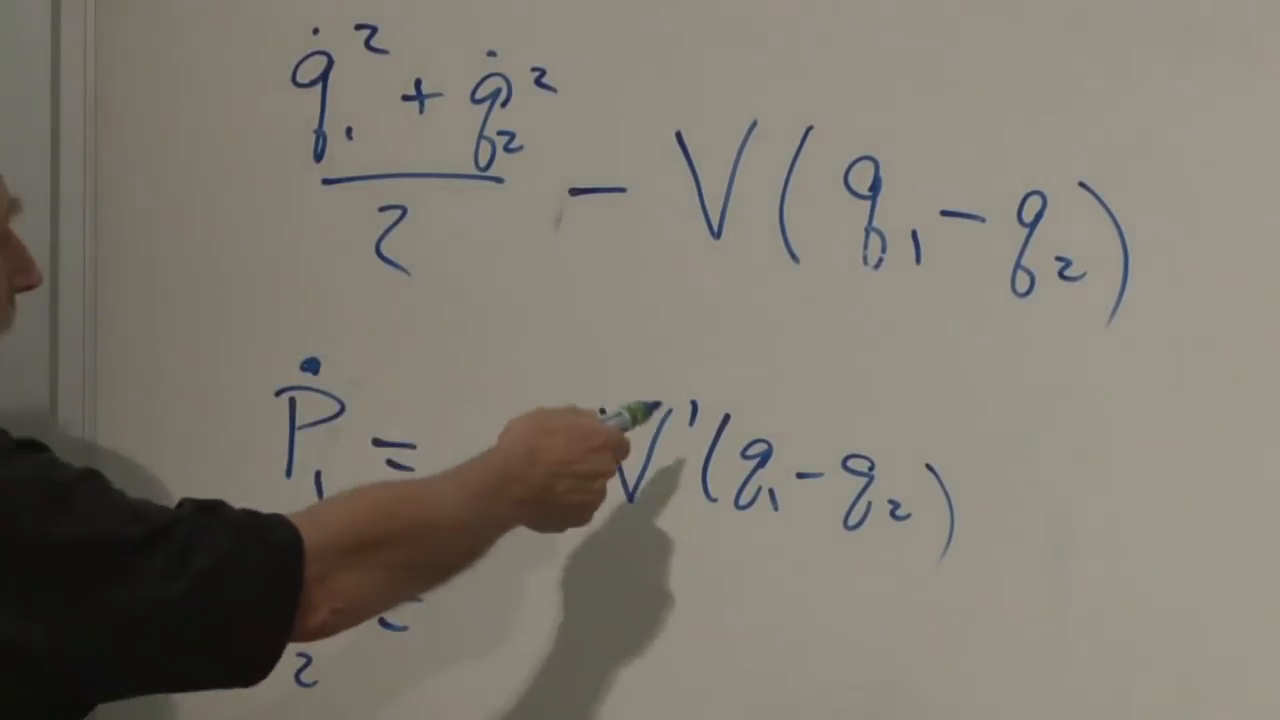
\includegraphics[width=0.78\textwidth]{lecture_04_figure_04.png}
  \caption{부호에 민감한 \(p_1\) 방정식의 미분. \(p_2\) 방정식에는 반대 부호가 붙는다.}
  \lectureframe{00:20:41}
\end{figure}

식 ~\eqref{eq:separation-momentum-equations}를 더하면
\begin{equation}
  \frac{d}{dt}(p_1+p_2)=0.
  \label{eq:total-p-conserved}
\end{equation}
보존량을 찾았지만, 그것이 왜 존재하는지는 아직 설명하지 않았다.

\subsection{덜 자명한 선형 결합}

이제
\begin{equation}
  L=\frac{\dot q_1^{\,2}+\dot q_2^{\,2}}{2}
    -V(Aq_1+Bq_2),
  \label{eq:ab-lagrangian}
\end{equation}
라 하자. 여기서 \(A\)와 \(B\)는 상수이다. 그러면
\begin{align}
  \dot p_1&=-A\,V'(Aq_1+Bq_2),
  \notag\\
  \dot p_2&=-B\,V'(Aq_1+Bq_2).
  \label{eq:ab-momentum-equations}
\end{align}
첫 번째 방정식에 \(B\)를 곱하고, 두 번째 방정식에 \(A\)를 곱한 뒤 두 식을 빼면 힘 항이 소거된다.
\begin{equation}
  \frac{d}{dt}(Bp_1-Ap_2)=0.
  \label{eq:ab-conserved}
\end{equation}

\begin{figure}[htbp]
  \centering
  \includegraphics[width=0.78\textwidth]{lecture_04_figure_06.png}
  \caption{가중 운동량 방정식에서 \(Bp_1-Ap_2\)의 힘 항들이 서로 상쇄된다.}
  \lectureframe{00:24:20}
\end{figure}

\begin{classroomqa}
  \audiencequestion{\(A\)와 \(B\) 같은 상수는 물리적으로 어디에서 올 수 있을까요?
  \lecturetimestamp{00:25:09--00:30:15}}
  \lecturerresponse{질량이 \(m\)와 \(M\)인 두 입자를 생각해 봅시다.
  \[
    L=\frac{m\dot X^2}{2}+\frac{M\dot Y^2}{2}-V(X-Y).
  \]
  \(Q_1=\sqrt m\,X\)와 \(Q_2=\sqrt M\,Y\)로 재척도화합시다. 운동에너지 항은 \((\dot Q_1^2+\dot Q_2^2)/2\)가 되고, 퍼텐셜은 \(Q_1/\sqrt m-Q_2/\sqrt M\)에 의존합니다. 따라서 질량이 서로 다르면 선형 결합의 계수에 자연스럽게 질량 인자가 들어갑니다. \(Q_2\)를 \(-Q_2\)로 바꾸면 제곱된 운동에너지 항은 그대로인 채 식에 표시된 마이너스 부호가 플러스 부호로 바뀝니다.}
\end{classroomqa}

\begin{figure}[htbp]
  \centering
  \includegraphics[width=0.82\textwidth]{lecture_04_figure_07.png}
  \caption{질량 가중 좌표는 운동에너지를 간단하게 만드는 대신 질량 인자를 퍼텐셜로 옮긴다.}
  \lectureframe{00:28:40}
\end{figure}

\begin{classroomqa}
  \audiencequestion{이로써 순환좌표가 없어도 보존량이 존재할 수 있음을 보인 건가요?
  \lecturetimestamp{00:31:13--00:31:58}}
  \lecturerresponse{현재 적힌 변수에는 \emph{명백한} 순환좌표가 없습니다. 변수 변환을 하면 순환좌표가 드러날 수 있지만, 그것을 찾아다니는 관점은 여기서 유용하지 않습니다. 대칭성 논증은 보존되는 결합을 직접 찾아낼 것입니다.}
\end{classroomqa}

\section{대칭의 의미}

\subsection{병진}

질량이 단위 질량인 자유 입자에서 시작하자.
\begin{equation}
  L=\frac{\dot q^2}{2}.
  \label{eq:free-unit-l4}
\end{equation}
그 운동 이력의 모든 점을 동일한 상수만큼 평행이동시키자.
\begin{equation}
  q'(t)=q(t)+\epsilon.
  \label{eq:free-translation}
\end{equation}
\(\epsilon\)는 시간에 무관하므로 \(\dot q'=\dot q\)이고, 따라서 \(\delta L=0\)이다. 이 변환은 병진 대칭이다.

서로 동등한 관점이 두 가지 있다. 수동적 관점에서는 물체를 그대로 둔 채 좌표 원점만 옮긴다. 능동적 관점에서는 좌표축을 고정하고 물체를 움직인다. 능동적 표현이 덜 혼란스럽다. 물리적 배치를 움직였을 때 \(L\)가 달라지는지 묻는 것이다.

식 ~\eqref{eq:separation-lagrangian}에 대해 두 좌표를 모두 병진시키자.
\begin{equation}
  \delta q_1=\epsilon,
  \qquad
  \delta q_2=\epsilon.
  \label{eq:common-translation}
\end{equation}
속도는 변하지 않으며 \(q_1-q_2\)도 변하지 않는다.

\begin{figure}[htbp]
  \centering
  \includegraphics[width=0.78\textwidth]{lecture_04_figure_08.png}
  \caption{두 좌표를 함께 병진시키면 두 좌표 사이의 간격은 변하지 않는다.}
  \lectureframe{00:35:30}
\end{figure}

식 ~\eqref{eq:ab-lagrangian}에 대해서는 덜 자명한 변환을 사용하자.
\begin{equation}
  \delta q_1=B\epsilon,
  \qquad
  \delta q_2=-A\epsilon.
  \label{eq:ab-transformation}
\end{equation}
이번에도 속도는 변하지 않으며,
\begin{equation}
  \delta(Aq_1+Bq_2)=AB\epsilon-BA\epsilon=0.
  \label{eq:ab-invariant-argument}
\end{equation}
따라서 이 변환은 대칭이다.

\begin{figure}[htbp]
  \centering
  \includegraphics[width=0.80\textwidth]{lecture_04_figure_09.png}
  \caption{를 보존하는 비대칭 병진.\(Aq_1+Bq_2\)}
  \lectureframe{00:40:20}
\end{figure}

\begin{classroomqa}
  \audiencequestion{이 계수들은 질량을 나타내며, 따라서 보존량은 보통의 질량중심 운동량이 되나요?
  \lecturetimestamp{00:42:25--00:42:45}}
  \lecturerresponse{그렇습니다. 질량 가중 변수에서는 대칭성과 보존되는 결합이 비대칭적으로 보입니다. 다시 \(X\)와 \(Y\)로 변환하면 보통의 동시 병진과 전체 운동량을 얻습니다.}
\end{classroomqa}

\subsection{회전}

평면에서 입자 하나를 생각하자.
\begin{equation}
  L=\frac{m}{2}(\dot x^2+\dot y^2)-V(x^2+y^2).
  \label{eq:central-lagrangian-l4}
\end{equation}
이는 중심 퍼텐셜이다. 서로 회전된 두 고정 좌표계를 비교하자. 좌표축은 시간에 따라 회전하지 않는다. 일관된 방향 규약을 택하면
\begin{align}
  x'&=x\cos\theta+y\sin\theta,
  \notag\\
  y'&=-x\sin\theta+y\cos\theta.
  \label{eq:finite-rotation-l4}
\end{align}

\begin{figure}[htbp]
  \centering
  \includegraphics[width=0.82\textwidth]{lecture_04_figure_10.png}
  \caption{중심 퍼텐셜을 가진 라그랑지안과 회전으로 서로 관계된 두 고정 데카르트 좌표계.}
  \lectureframe{00:45:40}
\end{figure}

\(\theta=\epsilon\)로 두고 1차 항까지만 남기자.
\begin{equation}
  \cos\epsilon=1+O(\epsilon^2),
  \qquad
  \sin\epsilon=\epsilon+O(\epsilon^3).
  \label{eq:small-angle-l4}
\end{equation}
무한소 회전은 다음과 같다.
\begin{align}
  \delta x&=y\epsilon,
  &\delta y&=-x\epsilon,
  \notag\\
  \delta\dot x&=\dot y\epsilon,
  &\delta\dot y&=-\dot x\epsilon.
  \label{eq:infinitesimal-rotation-l4}
\end{align}

\begin{figure}[htbp]
  \centering
  \includegraphics[width=0.82\textwidth]{lecture_04_figure_11.png}
  \caption{좌표와 속도의 무한소 회전.}
  \lectureframe{00:49:50}
\end{figure}

병진과 달리 \(x\)의 변화량은 \(y\)에 따라 달라지고, \(y\)의 변화량은 \(x\)에 따라 달라진다. 그럼에도
\begin{align}
  \delta(x^2+y^2)
  &=2x\,\delta x+2y\,\delta y=0,
  \notag\\
  \delta(\dot x^2+\dot y^2)
  &=2\dot x\,\delta\dot x+2\dot y\,\delta\dot y=0.
  \label{eq:rotation-invariants-l4}
\end{align}
퍼텐셜 항과 운동에너지 항은 모두 불변이다.

\begin{figure}[htbp]
  \centering
  \includegraphics[width=0.76\textwidth]{lecture_04_figure_12.png}
  \caption{제곱 반지름이 회전에 불변임을 보이는 1차 항의 상쇄.}
  \lectureframe{00:53:20}
\end{figure}

\section{일반적인 보존 정리}

병진과 회전의 예에는 공통된 형식이 있다. 연속적인 무한소 변환을 다음과 같이 두자.
\begin{equation}
  \delta q_i=\epsilon f_i(q),
  \qquad
  \delta\dot q_i=\frac{d}{dt}\delta q_i,
  \label{eq:general-infinitesimal-symmetry}
\end{equation}
여기서 \(\epsilon\)는 시간에 무관하며, \(f_i\)는 모든 좌표에 의존할 수 있다.

\begin{figure}[htbp]
  \centering
  \includegraphics[width=0.78\textwidth]{lecture_04_figure_13.png}
  \caption{일반적인 무한소 변위장 \(\delta q_i=\epsilon f_i(q)\)}
  \lectureframe{00:56:00}
\end{figure}

라그랑지안의 1차 변분은 다음과 같다.
\begin{equation}
  \delta L
  =\sum_i\left(
    \frac{\partial L}{\partial q_i}\delta q_i
    +\frac{\partial L}{\partial\dot q_i}\delta\dot q_i
  \right).
  \label{eq:delta-l-general}
\end{equation}

\begin{figure}[htbp]
  \centering
  \includegraphics[width=0.84\textwidth]{lecture_04_figure_14.png}
  \caption{\(\delta L\)에 기여하는 두 항: 좌표의 변분과 속도의 변분.}
  \lectureframe{01:02:30}
\end{figure}

이제 물리적 경로에 한정하면 오일러--라그랑주 방정식이 성립한다. 다음을 이용하면
\begin{equation}
  \frac{\partial L}{\partial\dot q_i}=p_i,
  \qquad
  \frac{\partial L}{\partial q_i}=\dot p_i,
  \label{eq:el-substitution-l4}
\end{equation}
다음 결과를 얻는다.
\begin{align}
  \delta L
  &=\sum_i\left(\dot p_i\,\delta q_i
                +p_i\,\delta\dot q_i\right)
  \notag\\
  &=\frac{d}{dt}\sum_i p_i\delta q_i
  =\epsilon\frac{d}{dt}\sum_i p_i f_i(q).
  \label{eq:noether-derivation-l4}
\end{align}
핵심 단계는 곱의 미분 법칙뿐이다.

변환이 대칭이면 \(\delta L=0\)이다. \(\epsilon\)는 임의의 상수 인자이므로
\begin{equation}
  \boxed{
  \frac{d\mathcal Q}{dt}=0,
  \qquad
  \mathcal Q=\sum_i p_i f_i(q)}
  .
  \label{eq:noether-charge-l4}
\end{equation}
이는 정확한 시간 독립 점 대칭에 대한 뇌터 정리의 고전역학적 핵심이다.

\begin{figure}[htbp]
  \centering
  \includegraphics[width=0.84\textwidth]{lecture_04_figure_15.png}
  \caption{곱의 미분 법칙을 이용해 \(L\)의 불변성으로부터 보존량을 얻는 단계.}
  \lectureframe{01:05:00}
\end{figure}

\begin{classroomqa}
  \audiencequestion{식 \(f_i(q)\)에서 \(q\)에 또 다른 첨자가 붙나요?
  \lecturetimestamp{01:06:57--01:07:31}}
  \lecturerresponse{첨자가 없는 \(q\)는 전체 집합 \((q_1,q_2,\ldots)\)를 뜻합니다. 각 성분 \(f_i\)는 그 좌표 전부에 의존할 수 있습니다. 예를 들어 회전의 경우 \(f_x=y\)이고 \(f_y=-x\)입니다.}
\end{classroomqa}

이제 예시들이 우연이 아님을 알 수 있다. 공통 병진에서는 \(f_1=f_2=1\)이므로
\begin{equation}
  \mathcal Q=p_1+p_2.
  \label{eq:noether-common-p}
\end{equation}
비대칭 병진에서는 \(f_1=B\), \(f_2=-A\)이므로
\begin{equation}
  \mathcal Q=Bp_1-Ap_2.
  \label{eq:noether-ab-p}
\end{equation}
회전에서는 \(f_x=y\)와 \(f_y=-x\)이므로
\begin{equation}
  \mathcal Q=p_xy-p_yx.
  \label{eq:rotation-charge-sign}
\end{equation}
방향 규약에 따른 부호 차이를 제외하면 이는 각운동량이다.
\begin{equation}
  J=xp_y-yp_x.
  \label{eq:angular-momentum-l4}
\end{equation}

\begin{figure}[htbp]
  \centering
  \includegraphics[width=0.82\textwidth]{lecture_04_figure_16.png}
  \caption{회전에 대한 뇌터 전하. 방향 규약에 따라 부호가 달라질 수 있지만 평면 각운동량과 같다.}
  \lectureframe{01:11:00}
\end{figure}

상호작용하는 입자가 여러 개라면 모든 입자를 함께 회전시킨다. 이때 불변성으로 보존되는 것은 각 입자의 각운동량이 따로가 아니라 각운동량의 합이다.

\section{정리의 가정에 관한 질문}

\begin{classroomqa}
  \audiencequestion{좌표축 집합을 회전시키면 \(\delta L\)에 명시적인 시간 의존성이 생기나요?
  \lecturetimestamp{01:12:57--01:13:57}}
  \lecturerresponse{그렇습니다. 방금 증명에서는 시간에 무관한 대칭 매개변수, 즉 고정된 병진이나 고정된 회전을 가정합니다. 매개변수가 시간에 의존하는 변환에는 추가 항이 생기므로 더 일반적인 처리가 필요합니다.}
\end{classroomqa}

\begin{classroomqa}
  \audiencequestion{칠판의 공식에 쓰인 대문자 \(Q\)가 변환 자체를 뜻하나요?
  \lecturetimestamp{01:14:02--01:15:58}}
  \lecturerresponse{아닙니다. 이 표기법은 안타깝게도 좌표 \(q_i\)와 겹칩니다. 변환은 \(\delta q_i=\epsilon f_i(q)\)이고, 그 결과 얻는 보존량은 \(\mathcal Q=\sum_i p_i f_i\)입니다. 계수 \(f_i\)는 대칭 변환 아래에서 \(i\)번째 좌표가 어떻게 움직이는지를 나타냅니다.}
\end{classroomqa}

에너지 보존도 대칭에서 비롯되지만, 다른 종류의 대칭이다. 시간에 대한 병진, 즉 시간의 원점을 어디에 두어도 물리가 달라지지 않는 성질이다. 이 경우와 해밀턴 형식은 뒤에서 다루겠다.

\begin{classroomqa}
  \audiencequestion{실제 운동을 변하는 좌표계에 흡수하여 역학을 좌표 변환만으로 설명할 수 있나요?
  \lecturetimestamp{01:17:43--01:20:01}}
  \lecturerresponse{특정한 운동을 따라가는 좌표를 선택할 수는 있지만, 그러면 그 변환은 초기 상태와 궤적에 의존합니다. 여기서 사용하는 대칭 변환은 계가 어떤 해를 따르는지와 무관하게 정해집니다. 운동 자체는 좌표와 운동량을 합친 공간에서 표현하는 편이 더 자연스럽습니다.}
\end{classroomqa}

\section{위상 공간에서의 조화 진동자}

질량과 용수철 상수를 각각 하나로 두면,
\begin{equation}
  L=\frac{\dot q^2}{2}-\frac{q^2}{2}.
  \label{eq:oscillator-l4}
\end{equation}
정준 운동량과 운동 방정식으로부터 다음을 얻는다.
\begin{equation}
  p=\dot q,
  \qquad
  \dot p=-q,
  \label{eq:oscillator-first-order-l4}
\end{equation}
또는
\begin{equation}
  \dot q=p,
  \qquad
  \dot p=-q.
  \label{eq:oscillator-phase-flow}
\end{equation}
이 방정식들은 \(q\)-\(p\) 평면에서의 등속 원운동을 나타낸다. 실제 공간에서 앞뒤로 진동하는 운동은 그 원을 \(q\)축에 투영한 것이다. 속력은 \(q=0\)에서 최대이고, 반전점에서는 사라진다.

\begin{figure}[htbp]
  \centering
  \includegraphics[width=0.82\textwidth]{lecture_04_figure_17.png}
  \caption{조화 진동자 방정식과 \(q\)-\(p\) 공간에서의 원형 궤도.}
  \lectureframe{01:25:30}
\end{figure}

\begin{classroomqa}
  \audiencequestion{위상 공간에서 원운동은 시계 방향인가요?
  \lecturetimestamp{01:25:47--01:27:15}}
  \lecturerresponse{가로축이 \(p\)이고 세로축이 \(q\)이면 그렇습니다. \(q\)가 양의 최댓값일 때 \(\dot p=-q<0\)이므로 운동은 아래쪽을 향합니다. 축의 배치를 반대로 하면 시각적인 회전 방향도 뒤집힙니다. 그래서 방향 규약을 잘못 기억하기 쉽습니다.}
\end{classroomqa}

식 ~\eqref{eq:oscillator-phase-flow}의 두 식은 이미 해밀턴 방정식과 닮았지만, 여기까지는 전적으로 라그랑주 역학 안에서 얻었다.

\section{연속 대칭과 이산 대칭}

\begin{classroomqa}
  \audiencequestion{대칭은 무한소 데카르트 변환으로 표현되어야 하나요?
  \lecturetimestamp{01:27:48--01:30:31}}
  \lecturerresponse{데카르트 좌표는 편리한 표현일 뿐이며, 이 증명에 본질적으로 필요한 조건은 연속성입니다. 무한소 표현이 없는 대칭도 있습니다. 퍼텐셜이 짝함수이면 반사는 \(q\mapsto -q\)와 \(\dot q\mapsto-\dot q\)를 변환하지만 \(L\)는 그대로 둡니다. 그러나 반사는 임의로 작은 반사들을 이어 붙여 만들 수 없습니다. 따라서 이 고전적 유도에서는 이에 대응하는 보존량을 얻지 못합니다.}
\end{classroomqa}

\begin{figure}[htbp]
  \centering
  \includegraphics[width=0.82\textwidth]{lecture_04_figure_18.png}
  \caption{짝함수 퍼텐셜은 이산 반사 \(q\mapsto -q\)에 불변이다.}
  \lectureframe{01:29:30}
\end{figure}

\begin{classroomqa}
  \audiencequestion{보존량 \(\mathcal Q\)이 영이 아니라면, 그 변환이 대칭이 아니었다는 뜻인가?
  \lecturetimestamp{01:30:40--01:31:30}}
  \lecturerresponse{아니다. 보존량은 어떤 상수값이든 가질 수 있다.
  관련된 판정 기준은 \(\dot{\mathcal Q}\)이다. 제안된 변환에서 유도한 양이 보존되지 않는다면, 증명의 가정 아래에서 그 변환은 대칭이 아니었던 것이다.}
\end{classroomqa}

\begin{classroomqa}
  \audiencequestion{반사해도 라그랑지안은 그대로인데, 왜 반사에서 보존 법칙이 나오지 않나요?
  \lecturetimestamp{01:31:34--01:32:27}}
  \lecturerresponse{불변성 자체는 확인할 수 있지만, 유도 과정은 1차 변위와 곱의 미분 법칙을 거쳤습니다. 반사는 배치 공간의 한쪽에서 다른 쪽으로 한 번의 이산적인 단계로 이동시킵니다. 무한소 생성자 \(f_i\)가 없으므로 공식 \(\mathcal Q=\sum_i p_i f_i\)을 적용할 대상이 없습니다.}
\end{classroomqa}

\begin{classroomqa}
  \audiencequestion{임의로 작은 변환들로 이루어진다는 성질은 무엇이라 부르나요?
  \lecturetimestamp{01:32:36--01:33:23}}
  \lecturerresponse{이를 \emph{연속 대칭}이라 합니다. 병진과 회전은 연속 대칭이고, 반사는 \emph{이산 대칭}입니다.}
\end{classroomqa}

\begin{classroomqa}
  \audiencequestion{무한소 단계들을 거쳐 유한 변환을 만들 때, 버린 \(O(\epsilon^2)\) 오차가 누적되지 않나요?
  \lecturetimestamp{01:33:23--01:36:10}}
  \lecturerresponse{무한소 불변성은 변환을 따라 도달하는 모든 점에서 성립해야 하며, 시작점에서만 성립해서는 안 됩니다. 유한한 매개변수 구간을 크기가 \(\epsilon\)인 \(N\)개의 단계로 나누면, 1차 변위의 누적량은 \(N\epsilon\)이고 국소적인 \(O(\epsilon^2)\) 나머지 항의 누적량은 \(N\epsilon^2=(N\epsilon)\epsilon\to0\)가 됩니다. 연속 변환군은 국소적인 성질에서 유한 변환으로 이어지는 이러한 구조를 형식화합니다.}
\end{classroomqa}

\begin{classroomqa}
  \audiencequestion{고전계에서 이산 대칭이 물리적으로 실현되기도 하나요?
  \lecturetimestamp{01:36:32--01:37:25}}
  \lecturerresponse{물론입니다. 조화 진동자 자체도 짝함수 퍼텐셜 \(V(q)\propto q^2\)을 가지므로 \(q\mapsto -q\)에 불변입니다. 이런 예는 많습니다. 여기서 말하고자 하는 것은 이 이산 불변성으로부터 새로운 고전적 뇌터 전하가 나오지는 않는다는 점뿐입니다.}
\end{classroomqa}

\begin{classroomqa}
  \audiencequestion{연속 변환과 이산 변환이 모두 \(L\)를 그대로 둔다면, 같은 조건 아닌가요?
  \lecturetimestamp{01:37:37--01:39:18}}
  \lecturerresponse{불변성에 대한 유한한 진술은 같지만, 이 증명에 필요한 수학적 입력은 같지 않습니다. 증명에는 1차 변분이 필요합니다. 반사에는 ‘1차’라는 개념이 적용되지 않으므로, 보존량으로 이어지는 식들의 연쇄를 시작조차 할 수 없습니다.}
\end{classroomqa}

\begin{classroomqa}
  \audiencequestion{역사적으로 뇌터 정리와는 어떤 관계가 있나요?
  \lecturetimestamp{01:39:26--01:40:42}}
  \lecturerresponse{여기서 다룬 것은 에미 뇌터의 훨씬 더 일반적인 정리 중 제한된 부분입니다. 대칭과 보존량 사이의 구체적인 관계들은 이전에도 알려져 있었지만, 뇌터는 20세기 초에 이를 통합된, 놀라울 만큼 일반적인 틀로 정립했습니다. 그녀의 수학적 업적에 걸맞은 공정한 학문적 대우는 받지 못했습니다.}
\end{classroomqa}

\begin{classroomqa}
  \audiencequestion{고전역학은 지금도 활발한 연구 분야인가요?
  \lecturetimestamp{01:40:47--01:42:37}}
  \lecturerresponse{그렇습니다. 여기서 사용한 기초적인 정리는 오래되었지만, 비선형 동역학, 적분 가능한 계, 혼돈, 유체, 기하학적 역학은 여전히 풍부한 연구 분야입니다. 대칭성 원리는 고전 입자역학을 훨씬 넘어 계속 적용됩니다.}
\end{classroomqa}

\section{작용 원리가 중요한 이유}

\begin{classroomqa}
  \audiencequestion{대칭성이 보존을 뜻하는 직관적인 이유가 있나요?
  \lecturetimestamp{01:42:49--01:47:57}}
  \lecturerresponse{대칭성만으로는 그렇지 않습니다. 점성 저항을 생각해 봅시다.
  \[
    m\ddot x=-c\dot x.
  \]
  이 방정식은 \(x\mapsto x+\epsilon\)에 불변이지만, \(p=m\dot x\)일 때
  \[
    \dot p=-\frac{c}{m}p,
    \qquad
    p(t)=p(0)e^{-ct/m},
  \]
  운동량은 감소합니다. 이는 계 전체를 나타내는 근본적인 정지 작용 법칙이 아니라, 부분계에 대한 유효 방정식입니다. 유체 분자와 닫힌 계의 나머지 부분까지 포함하면 전체 운동량은 보존됩니다. 대칭성과 보존은 미분 방정식의 형태 자체가 아니라 라그랑지안 작용 원리를 통해 연결됩니다.\(x\)만의 경우가 그렇습니다.}
\end{classroomqa}

\begin{figure}[htbp]
  \centering
  \includegraphics[width=0.65\textwidth]{lecture_04_figure_19.png}
  \caption{병진 불변인 점성 저항에서는 입자 운동량이 줄어든다.}
  \lectureframe{01:44:30}
\end{figure}

\begin{classroomqa}
  \audiencequestion{물리적 경로가 작용의 최소가 아닌 경우를 정량적으로 설명할 수 있나요?
  \lecturetimestamp{01:48:08--01:51:38}}
  \lecturerresponse{진정한 최소는 드물며, 작용은 일반적으로 경로 공간에서 안장점이다. 단위 질량 조화 진동자의 경우
  \[
    S[q]=\frac12\int(\dot q^2-q^2)\,dt.
  \]
  폭이 좁고 빠르게 변하는 변형은 양의 \(\dot q^2\) 항을 증가시킵니다. 조금 벗어난 상태를 오랫동안 유지하는 완만한 변형은 음의 \(-q^2\) 항이 지배하게 만들어 작용을 낮출 수 있습니다. 따라서 같은 정지 경로에도 작용을 증가시키는 방향과 감소시키는 방향이 있습니다. 양자역학은 경로 적분 관점을 통해 정지성의 더 깊은 근원을 설명하지만, 그 논의는 뒤로 미루겠습니다.}
\end{classroomqa}

\begin{figure}[htbp]
  \centering
  \includegraphics[width=0.80\textwidth]{lecture_04_figure_20.png}
  \caption{완만하게 벗어난 조화 진동자 경로는 정지 작용이 최소라기보다 안장점인 경우가 보통임을 보여 준다.}
  \lectureframe{01:50:20}
\end{figure}

\begin{classroomqa}
  \audiencequestion{연속 대칭과 보존 법칙은 일대일 대응하나요?
  \lecturetimestamp{01:51:44--01:52:43}}
  \lecturerresponse{변분적 틀 안에서 동등하거나 자명한 경우를 구별하면, 대체로 그렇게 이해해도 됩니다. 모든 연속 대칭에는 전하가 있고, 보존량은 일반적으로 대칭과 연결할 수 있습니다. 정확한 진술에는 기술적인 한정 조건이 따르므로, 이 포괄적인 설명을 부주의하게 사용해서는 안 됩니다.}
\end{classroomqa}

\begin{classroomqa}
  \audiencequestion{모든 라그랑지안에는 자명하지 않은 대칭이 있어야 하나요?
  \lecturetimestamp{01:52:43--01:53:23}}
  \lecturerresponse{아닙니다. 여기서는 대칭이 있는 예들을 골랐습니다. 일반적인 라그랑지안은 제안된 어떤 공간 변환에도 불변일 필요가 없습니다.}
\end{classroomqa}

\begin{classroomqa}
  \audiencequestion{대칭은 결국 능동적인 운동으로 이해해야 하나요, 아니면 수동적인 좌표 변환으로 이해해야 하나요?
  \lecturetimestamp{01:53:25--01:55:08}}
  \lecturerresponse{두 설명은 서로 동등하게 만들 수 있지만, 여기서는 능동적 설명이 더 간결합니다. 물리적 계 전체를 움직이고 라그랑지안이 변하는지 묻습니다. 수동적 표현에서는 좌표계가 움직일 때 라그랑지안의 \emph{형식}이 변하지 않는다고 말해야 합니다.}
\end{classroomqa}

\begin{classroomqa}
  \audiencequestion{다음에는 무엇을 다루나요?
  \lecturetimestamp{01:55:10--01:55:35}}
  \lecturerresponse{에너지 보존과 그것의 시간 병진 대칭에서의 기원, 그리고 해밀턴 형식입니다.}
\end{classroomqa}\chapter{에너지와 해밀토니안}

\lectureoverview{먼저 능동 대칭의 의미를 더 정확히 규정하고, 병진과 회전이 운동량과 각운동량을 어떻게 생성하는지 살펴본다. 빠져 있던 보존량은 에너지다. 에너지에 대응하는 대칭은 시간 병진이며, 그 보존량은 해밀토니안 \(H=\sum_i p_i\dot q_i-L\)이다. 이 유도 과정은 명시적인 시간 의존성이 선택한 부분계와 그 환경 사이에서 에너지를 어떻게 전달하는지도 정확히 보여 준다.}

\section{정식 논증에 앞서 나온 질문}

이후 주제를 다루는 데 필요한 고전역학의 최소한에 가까워지고 있지만, 더 배울 가치가 있는 역학은 아직 많이 남아 있다. 본격적인 논증에 앞서 두 가지 질문이 나왔다.

\begin{classroomqa}
  \audiencequestion{이 입문 강의 다음에는 어떤 책이 도움이 되나요?
  \lecturetimestamp{00:00:36--00:02:13}}
  \lecturerresponse{널리 쓰이는 고급 참고서는 Herbert Goldstein의 \emph{고전역학}이다. 역학의 변분 원리를 다룬 Cornelius Lanczos의 책도 관련 참고 자료다. 한 강사가 이용 가능한 모든 교재를 훑어볼 수 있다고 가장하기보다는 강의용 독서 목록을 참고하는 편이 더 유용하다.}
\end{classroomqa}

두 번째 질문에는 아직 해결되지 않은 측정 문제의 당시 상황이 담겨 있다. 2011년에 OPERA 실험은 CERN에서 Gran Sasso로 보낸 중성미자가 예상보다 일찍 도착한 듯한 결과를 보고했다. 보고된 시간 차이는 중성미자를 만들 때 사용한 양성자 펄스보다 짧았다. 따라서 시간 분석에서는 중성미자가 방출될 때 하나를 표시해 두었다가 검출 시 같은 입자인지 확인하는 대신 펄스의 시간 분포를 비교해야 했다.

\begin{classroomqa}
  \audiencequestion{빛보다 빠른 중성미자라는 결과는 해결되었나요?
  \lecturetimestamp{00:02:30--00:09:03}}
  \lecturerresponse{당시에는 어떤 결론도 내릴 근거가 없었다. 빔 펄스의 형태, 표적의 가열, 동기화 문제를 모두 기술적으로 면밀히 검토해야 했다. 한 가지 추측성 제안에서는 GPS 위성의 운동을 고려했다. 위성 좌표계에서는 시간 신호가 전달되는 동안 발생원과 검출기가 움직이므로 수십 나노초 정도의 보정이 생긴다는 것이었다. 이 추산은 차수 크기를 따져 보는 연습으로는 흥미로웠지만, 실험 결과를 그럴듯하게 진단한 것으로 제시되지는 않았다. 해당 속도에서의 통상적인 로런츠 수축은 보고된 효과를 설명하기에 너무 작았다. 적절한 대응은 실험 분석을 기다리는 것이었다.}
\end{classroomqa}

\begin{figure}[htbp]
  \centering
  \includegraphics[width=0.78\textwidth]{lecture_05_figure_07.png}
  \caption{역사적 중성미자 측정 문제를 논의하며 살펴본 위성 좌표계의 시간 측정 도식.}
  \lectureframe{00:06:30}
\end{figure}

시간 측정에 관한 논의는 아래 역학 내용을 이해하는 데 필요하지 않다. 하지만 그럴듯한 규모 추산과 확립된 실험적 설명은 서로 다르다는 점을 상기시켜 준다.

\section{능동 대칭과 계의 선택}

앞선 논의에서 충분히 명확히 다루지 못한 문제로 돌아가 보자. 대칭이란 정확히 무엇인가? 직선 위의 입자와 다음 지시를 생각하자.
\begin{equation}
  x\longrightarrow x+1.
  \label{eq:l5-shift-one}
\end{equation}
이를 이해하는 방법은 두 가지다. \emph{수동} 변환은 직선 위의 점에 붙인 이름을 다시 정하는 것이다. 한때 \(x=0\)이라고 부르던 점을 이제 \(x'=1\)이라고 부를 수 있지만, 입자가 움직인 것은 아니다. \emph{능동} 변환은 표지를 그대로 둔 채 입자 자체를 \(x\)에서 \(x+1\)로 이동시킨다. 외부 퍼텐셜에 대한 입자의 위치를 바꾸는 것은 두 번째 작용뿐이다.

\begin{figure}[htbp]
  \centering
  \includegraphics[width=0.82\textwidth]{lecture_05_figure_08.png}
  \caption{규칙 \(x\mapsto x+1\), 고정된 좌표축, 외부 퍼텐셜을 이용하면 능동적 운동과 수동적 표지 재설정을 구별할 수 있다.}
  \lectureframe{00:11:20}
\end{figure}

\begin{classroomqa}
  \audiencequestion{입자를 움직여 퍼텐셜 에너지가 달라진다면, 그 퍼텐셜의 발생원은 계에서 제외한 건가요?
  \lecturetimestamp{00:12:19--00:14:18}}
  \lecturerresponse{그렇다. 계를 ``퍼텐셜 안의 입자''라고 부르면, 세계를 입자와 퍼텐셜 \(V(x)\)를 만들어 내는 지구 같은 무거운 환경으로 나누는 것이다. 지구도 반동하지만, 이 근사에서는 질량이 엄청나게 커서 그 반동을 무시할 수 있다. 고정된 지구에 대해 입자를 움직이면 \(V\)가 달라질 수 있지만, 입자와 지구를 함께 병진시키면 달라지지 않는다.}
\end{classroomqa}

\begin{classroomqa}
  \audiencequestion{앞서 회전을 예로 들었을 때 위치뿐 아니라 속도도 바뀌었나요?
  \lecturetimestamp{00:14:26--00:15:29}}
  \lecturerresponse{그렇다. 강체의 능동 회전은 한 순간의 위치에만 작용하는 것이 아니라 전체 이력에 작용한다. 위치 벡터와 속도 벡터가 모두 회전한다. 반면 모든 시각에 똑같이 적용하는 상수 병진은 \(x\)를 바꾸지만 \(\dot x\)는 바꾸지 않는다.}
\end{classroomqa}

계와 환경의 구분은 두 번 더 등장한다. 시간에 따라 변하는 장치가 부분계와 에너지를 주고받을 때, 그리고 거시적 마찰 때문에 관측되지 않는 미시적 운동에 에너지가 숨을 때다.

\section{배치 공간에서의 무한소 운동}

일반적인 역학계의 배치는 일반화 좌표 \(q_i\) 공간의 한 점이다. 능동적인 무한소 변환은 가능한 모든 배치를 그에 가까운 배치로 옮긴다. 이를 다음과 같이 쓴다.
\begin{equation}
  \delta q_i=\epsilon f_i(q),
  \label{eq:l5-general-transformation}
\end{equation}
함수 \(f_i\)는 배치 공간에서 하나의 고정된 변위장을 지정한다. 이 함수들은 모든 좌표에 의존할 수 있으며, 일부는 사라질 수 있다. 공통 인자 \(\epsilon\)는 작으며, 변환 단계의 크기와 변환의 형태를 분리한다.

\begin{figure}[htbp]
  \centering
  \includegraphics[width=0.75\textwidth]{lecture_05_figure_09.png}
  \caption{배치 공간의 각 점에 붙인 변위 벡터.}
  \lectureframe{00:16:50}
\end{figure}

\begin{figure}[htbp]
  \centering
  \includegraphics[width=0.80\textwidth]{lecture_05_figure_10.png}
  \caption{좌표에 따라 달라지는 무한소 변환 \(\delta q_i=\epsilon f_i(q)\).}
  \lectureframe{00:18:00}
\end{figure}

변환 규칙 자체에는 명시적인 시간 의존성이 없다. 따라서 속도에 작용하는 변환은 다음과 같다.
\begin{equation}
  \delta\dot q_i=\frac{d}{dt}(\delta q_i)
  =\epsilon\sum_j\frac{\partial f_i}{\partial q_j}\dot q_j.
  \label{eq:l5-velocity-variation}
\end{equation}
병진에서는 \(f_x=1\)이므로 \(\delta\dot x=0\)이다. 회전에서는 \(f_i\)가 위치에 따라 달라지므로 속도도 변한다.

\begin{classroomqa}
  \audiencequestion{마지막의 작은 인자 \(\delta q_i=\epsilon f_i(q)\)는 모든 점에서 같은 상수인가요?
  \lecturetimestamp{00:19:58--00:20:51}}
  \lecturerresponse{그렇다. 하나의 상수 \(\epsilon\)는 모든 좌표 변화가 동일한 작은 양의 1차가 되도록 하는 표기상의 장치다. 공간 의존성은 \(f_i(q)\)에 들어 있으며, \(\epsilon\)에는 들어 있지 않다. 이 함수들 자체는 작을 필요가 없다.}
\end{classroomqa}

\section{변환이 대칭이 되는 조건}

능동 변환은 일반적으로 퍼텐셜 에너지를 바꾼다. 운동에너지도 바뀔 수 있다. 곡선좌표에서 운동에너지 항은 다음 형태를 갖는다.
\begin{equation}
  T=\frac12\sum_{i,j}g_{ij}(q)\dot q_i\dot q_j,
  \label{eq:l5-kinetic-metric}
\end{equation}
따라서 배치 공간에서 움직이면 그 계수가 달라질 수 있다. 극좌표에서 익숙한 \(r^2\dot\theta^2\) 항이 가장 간단한 예다.

여기서 변환이 대칭이라는 것은 \emph{전체} 라그랑지안의 변화가 1차에서 사라진다는 뜻이다.
\begin{equation}
  \delta L=O(\epsilon^2),
  \label{eq:l5-symmetry-condition}
\end{equation}
이 조건은 특정한 해 하나가 점유하는 배치에서만이 아니라 배치 공간의 모든 점에서 성립해야 한다.

예를 들어, \(x\mapsto x+\epsilon\) 변환에서는
\begin{equation}
  \delta V=\frac{\partial V}{\partial x}\epsilon.
  \label{eq:l5-potential-variation}
\end{equation}
이 값이 가능한 모든 \(x\)에 대해 사라진다면,
\(\partial V/\partial x=0\)이다. 즉, 퍼텐셜은 \(x\)에 의존하지 않는다. 모든 공간 방향의 병진 변환에도 퍼텐셜이 변하지 않는다면, 퍼텐셜은 상수이다.

\begin{figure}[htbp]
  \centering
  \includegraphics[width=0.80\textwidth]{lecture_05_figure_11.png}
  \caption{\(x\) 병진을 \(x\)에 의존하지 않는 퍼텐셜 \(V(y)\)에 적용한 경우.}
  \lectureframe{00:23:40}
\end{figure}

매끄러운 1매개변수 군에서는 모든 점에서 1차 변화가 사라지므로, 무한소 단계를 이어 붙여 유한 대칭을 만들 수 있다.

\begin{classroomqa}
  \audiencequestion{운동에너지와 퍼텐셜 에너지가 각각 따로 불변이어야 하나요?
  \lecturetimestamp{00:24:44--00:25:33}}
  \lecturerresponse{아니다. 불변이어야 하는 것은 전체 라그랑지안뿐이다. 일부 라그랑지안에는 좌표와 속도가 섞인 항이 들어 있어 --, \(T\), \(V\)로 유용하게 분리할 수 없다. 그러므로 각 항의 불변성을 따지는 질문 자체가 의미 없을 수도 있다.}
\end{classroomqa}

\begin{classroomqa}
  \audiencequestion{``변화가 없다''는 말은 정확히 변화가 없다는 뜻인가요, 아니면 무시할 만큼 작다는 뜻인가요?
  \lecturetimestamp{00:25:34--00:28:59}}
  \lecturerresponse{무한소 변환에서는 \(\epsilon\)에 비례하는 항이 없다는 뜻이다. 국소 계산에서는 \(\epsilon^2\) 차수의 항을 버린다. 1차 조건이 1매개변수 궤도를 따라 모든 점에서 성립하므로 국소 단계를 반복하면 유한 불변성이 얻어진다.}
\end{classroomqa}

\section{운동량과 각운동량의 재도출}

여기서 다루는 정확한 시간 독립 점 대칭에 대해 앞서 증명한 결과는 다음과 같다.
\begin{equation}
  Q=\sum_i p_i f_i(q),
  \qquad
  p_i=\frac{\partial L}{\partial\dot q_i},
  \qquad
  \dot Q=0.
  \label{eq:l5-noether-charge}
\end{equation}
인자 \(\epsilon\)는 \(Q\)에 포함되지 않는다. 대칭 궤도를 따라 얼마나 이동하는지를 나타낼 뿐이다.

\begin{figure}[htbp]
  \centering
  \includegraphics[width=0.82\textwidth]{lecture_05_figure_12.png}
  \caption{일반적인 무한소 변위와 이에 대응하는 보존 노에터 전하.}
  \lectureframe{00:30:00}
\end{figure}

\(x\) 방향 병진에서는 \(f_x=1\)이고 \(Q=p_x\)이다. 모든 병진 대칭이 성립하면 운동량의 세 성분이 모두 보존된다. 서로 상호작용하는 입자가 여러 개일 때는 모든 입자를 함께 병진시키는 것이 대칭이다. 상호작용이 상대 위치에만 의존하면 \begin{equation}
  \mathbf P=\sum_a\mathbf p_a
  \label{eq:l5-total-momentum}
\end{equation}가 보존된다. 입자 하나만 나머지 입자에 대해 움직이는 것은 대칭이 아니다.

\begin{figure}[htbp]
  \centering
  \includegraphics[width=0.80\textwidth]{lecture_05_figure_13.png}
  \caption{함께 병진시키면 운동량의 각 성분이 보존되어 총운동량이 보존된다.}
  \lectureframe{00:32:50}
\end{figure}

\(x\)-\(y\) 평면에서 무한소 회전을 생각하고, 회전 방향을 다음과 같이 정한다.
\begin{equation}
  \delta x=-y\epsilon,
  \qquad
  \delta y=x\epsilon.
  \label{eq:l5-planar-rotation}
\end{equation}
다음 식에서 알 수 있듯이 반지름은 보존된다.
\begin{equation}
  \delta(x^2+y^2)
  =2x\delta x+2y\delta y=0.
  \label{eq:l5-radius-invariance}
\end{equation}

\begin{figure}[htbp]
  \centering
  \includegraphics[width=0.76\textwidth]{lecture_05_figure_14.png}
  \caption{평면 무한소 회전의 기하학적 의미와 좌표 표현.}
  \lectureframe{00:35:05}
\end{figure}

식~\eqref{eq:l5-planar-rotation}을 미분하면 속도도 함께 회전한다. 따라서 \(\dot x^2+\dot y^2\)는 불변이고, 중심 퍼텐셜 \(V(\sqrt{x^2+y^2})\)은 라그랑지안 전체를 변하지 않게 한다. 이에 대응하는 전하는 다음과 같다.
\begin{equation}
  Q=-yp_x+xp_y=(\mathbf r\times\mathbf p)_z.
  \label{eq:l5-angular-charge}
\end{equation}

\begin{figure}[htbp]
  \centering
  \includegraphics[width=0.76\textwidth]{lecture_05_figure_15.png}
  \caption{회전에 대응하는 노에터 전하, 즉 각운동량의 \(z\) 성분.}
  \lectureframe{00:38:50}
\end{figure}

다른 좌표 평면에서의 회전은 나머지 성분을 준다. 여러 입자에 대해 보존되는 벡터는 다음과 같다.
\begin{equation}
  \mathbf J=\sum_a\mathbf r_a\times\mathbf p_a.
  \label{eq:l5-total-angular-momentum}
\end{equation}
중심 별의 퍼텐셜 안에서 움직이는 행성이 기본적인 예다. 모든 회전에 대한 불변성은 각운동량의 모든 성분이 보존됨을 뜻한다.

\begin{classroomqa}
  \audiencequestion{한쪽에서의 미분값과 다른 쪽에서의 미분값이 다른 뾰족한 첨점에서는 어떻게 되나요?
  \lecturetimestamp{00:42:25--00:44:21}}
  \lecturerresponse{타당한 지적입니다. 현재 논증은 미분 가능하고 도함수가 유일하게 정해지는 함수를 가정합니다. 매끄러운 극댓값 위에 놓인 물체처럼 불안정한 평형은 그 자체로 문제가 되지 않습니다. 그 점에서 도함수가 존재하고 사라지기 때문입니다. 실제 첨점을 다루려면 논증을 수정해야 합니다.}
\end{classroomqa}

\begin{classroomqa}
  \audiencequestion{변환 매개변수가 시간에 무관한데 회전하면 왜 속도가 바뀌나요?
  \lecturetimestamp{00:44:23--00:45:23}}
  \lecturerresponse{매개변수는 상수지만 변위장은 좌표에 의존한다. 일반적인 규칙은 \(\delta\dot q_i=d(\delta q_i)/dt\)이다. 병진에서는 \(\delta x\)가 상수지만 회전에서는 \(\delta x=-y\epsilon\)이므로 \(\delta\dot x=-\dot y\epsilon\)이다.}
\end{classroomqa}

\section{초등적인 운동에너지 빼기 퍼텐셜 에너지 형식을 넘어}

자기장이 없는 비상대론적 입자를 직교좌표로 나타내면 \(L=T-V\)이다. 더 일반적인 좌표에서는 식~\eqref{eq:l5-kinetic-metric}의 이차형식이 나온다. 자기장이 있으면 속도에 선형인 항, 개략적으로 \(\mathbf A(q)\cdot\dot{\mathbf q}\)가 들어가 좌표와 속도가 서로 섞인다. 이런 경우에는 모든 항을 통상적인 운동에너지와 퍼텐셜 에너지로 억지로 나누기보다 \(L(q,\dot q,t)\)를 하나의 함수로 다루는 편이 낫다.

\begin{figure}[htbp]
  \centering
  \includegraphics[width=0.80\textwidth]{lecture_05_figure_16.png}
  \caption{좌표에만 의존하는 퍼텐셜과 일반적인 좌표 의존 이차 운동에너지 항.}
  \lectureframe{00:47:20}
\end{figure}

\begin{classroomqa}
  \audiencequestion{라그랑지안이 운동에너지와 퍼텐셜 에너지로 깔끔히 분리되지 않을 수 있는 이유는 무엇인가요? 그래도 라그랑지안은 \(T-V\)로 정의되나요?
  \lecturetimestamp{00:45:26--00:48:13}}
  \lecturerresponse{장애물은 곡선좌표에서 비롯될 수도 있고, 자기력처럼 실제 속도 의존 상호작용에서 생길 수도 있다. 라그랑지안이 속도에 대한 이차형식에서 좌표에만 의존하는 함수를 뺀 형태일 때에만 두 항을 \(T\)와 \(V\)라고 부른다. 그렇지 않아도 라그랑지안은 여전히 \(q\)와 \(\dot q\)의 함수로서 완전히 타당하지만, 그렇게 나누는 것은 별로 유용하지 않다. 에너지의 올바른 일반적 정의는 해밀토니안에서 나온다.}
\end{classroomqa}

\begin{classroomqa}
  \audiencequestion{첫 모임에서 다룬 늘어진 사슬 예제는 최소작용 원리를 적용한 것이었나요?
  \lecturetimestamp{00:48:15--00:49:45}}
  \lecturerresponse{그 예제는 최소에너지로 정해지는 평형 문제였지, 정지작용으로 선택되는 이력 문제는 아니었다. 통상적인 \(T-V\) 계의 정적 해에서는 \(\dot p_i=0\)이므로 오일러--라그랑주 방정식은 퍼텐셜의 정지점 조건인 \(\partial V/\partial q_i=0\)로 줄어든다.}
\end{classroomqa}

운동량과 각운동량은 이제 공간 대칭과 연결되었다. 뚜렷하게 빠져 있는 양은 에너지다.

\section{시간 병진 불변성}

\(t_0\)에 시작해 \(t_1\)에 끝나며 어떤 결과를 내는 실험을 생각하자. 같은 준비를 한 뒤, 더 늦은 시점인 \(t_0+\Delta t\)에 시작해 \(t_1+\Delta t\)에 끝나도록 반복한다. 결과가 변하지 않는다면 그 계는 시간에 대한 능동 병진에 불변이다.

\begin{figure}[htbp]
  \centering
  \includegraphics[width=0.82\textwidth]{lecture_05_figure_17.png}
  \caption{배치 공간의 이력 안에서 실험과 이를 시간 병진시킨 실험을 나타낸 그림.}
  \lectureframe{00:52:45}
\end{figure}

축전기 판 사이의 하전 입자는 이 대칭이 깨지는 예다. 판의 전하가 고정되어 있다면 같은 실험을 언제든 수행할 수 있다. 외부 발전기가 판을 계속 충전한다면, 입자가 방출되는 시점에 따라 입자가 경험하는 전기장이 달라진다. 이때 입자는 명시적으로 구동되는 부분계다.

\begin{figure}[htbp]
  \centering
  \includegraphics[width=0.82\textwidth]{lecture_05_figure_18.png}
  \caption{시간 병진 도식 옆에 대비해 그린, 전하가 고정된 축전기 판과 외부 작용으로 변하는 축전기 판.}
  \lectureframe{00:54:45}
\end{figure}

진동자에서도 같은 점을 볼 수 있다.
\begin{equation}
  L=\frac12m\dot x^2-\frac12k(t)x^2.
  \label{eq:l5-driven-oscillator}
\end{equation}
외부 전기장이나 자기장이 물질을 서서히 변화시켜 유효 용수철 상수를 바꿀 수 있다. \(k\)가 변하면 진동자 실험을 시간상으로 옮겼을 때 결과가 달라진다.

\begin{figure}[htbp]
  \centering
  \includegraphics[width=0.78\textwidth]{lecture_05_figure_19.png}
  \caption{시간에 따라 용수철 상수가 변하는 경우를 논의하며 살펴본 진동자의 운동에너지 항과 퍼텐셜 에너지 항.}
  \lectureframe{00:56:45}
\end{figure}

\(k\)를 변화시키는 장치를 계에 포함하면 전체 폐쇄계 실험을 다시 시간 병진시킬 수 있고 전체 에너지는 보존된다. 에너지가 보존되지 않는 듯 보이는 것은 우리가 정한 경계를 가로질러 에너지가 교환되기 때문이다.

휴식 시간에 작은 변환 매개변수의 이름을 \(\epsilon\)로 바꾸어, 시각적으로 혼동을 일으키는 표현 \(\delta x=\delta\)를 피했다. 에이미 뇌터에 관한 책도 강의용 독서 목록에 넣도록 추천했다.

\begin{classroomqa}
  \audiencequestion{라그랑지안이 \(T-V\) 형태로 주어지지 않는다면 어디서 얻나요?
  \lecturetimestamp{01:00:17--01:02:24}}
  \lecturerresponse{실험으로 추론하거나, 알려진 운동 방정식에서 재구성하거나, 대칭과 다른 이론적 원리에 근거해 추측하거나, 시행착오로 찾을 수 있다. \(L(q,\dot q,t)\)가 주어지면 오일러--라그랑주 계산을 통해 운동 방정식을 얻는다. 정식 논증을 위해 라그랑지안의 기원을 먼저 확정할 필요는 없다.}
\end{classroomqa}

시간 병진 불변성의 조작적 판정은 이제 간단하다. \(q\)와 \(\dot q\)만으로 \(L\)를 정할 수 있고 시계의 시각은 알 필요가 없다면,
\begin{equation}
  \frac{\partial L}{\partial t}=0.
  \label{eq:l5-no-explicit-time}
\end{equation}
이는 \(L(q(t),\dot q(t))\)이 운동 중 일정하다는 뜻이 아니다. 시간에 대한 의존성이 변화하는 좌표와 속도를 통해 나타나는 것 외에는 없다는 뜻이다.

회전하는 무거운 아령도 구동되는 계의 예다. 아령의 운동이 가벼운 시험 입자에 시간에 따라 변하는 중력 퍼텐셜을 만든다면 시험 입자의 라그랑지안은 시간에 명시적으로 의존한다. 아령을 동역학적으로 다루면 계가 확장되어 외부 시간 의존성이 사라진다.

\begin{figure}[htbp]
  \centering
  \includegraphics[width=0.80\textwidth]{lecture_05_figure_20.png}
  \caption{정해진 운동을 하는 회전 아령이 더 가벼운 입자의 시간 의존 외부 발생원으로 작용한다.}
  \lectureframe{01:06:25}
\end{figure}

\section{해밀토니안의 유도}

에너지 공식을 모른다고 가정하고 라그랑지안 자체가 보존될 것이라고 추측해 보자. 이를 직접 확인하려면 실제 궤적을 따라 라그랑지안을 미분하면 된다. 간단히 먼저 명시적인 시간 의존성이 없는 경우부터 시작하자.
\begin{equation}
  \frac{dL}{dt}
  =\sum_i\left(
    \frac{\partial L}{\partial q_i}\dot q_i
    +\frac{\partial L}{\partial\dot q_i}\ddot q_i
  \right).
  \label{eq:l5-chain-rule-no-time}
\end{equation}

\begin{figure}[htbp]
  \centering
  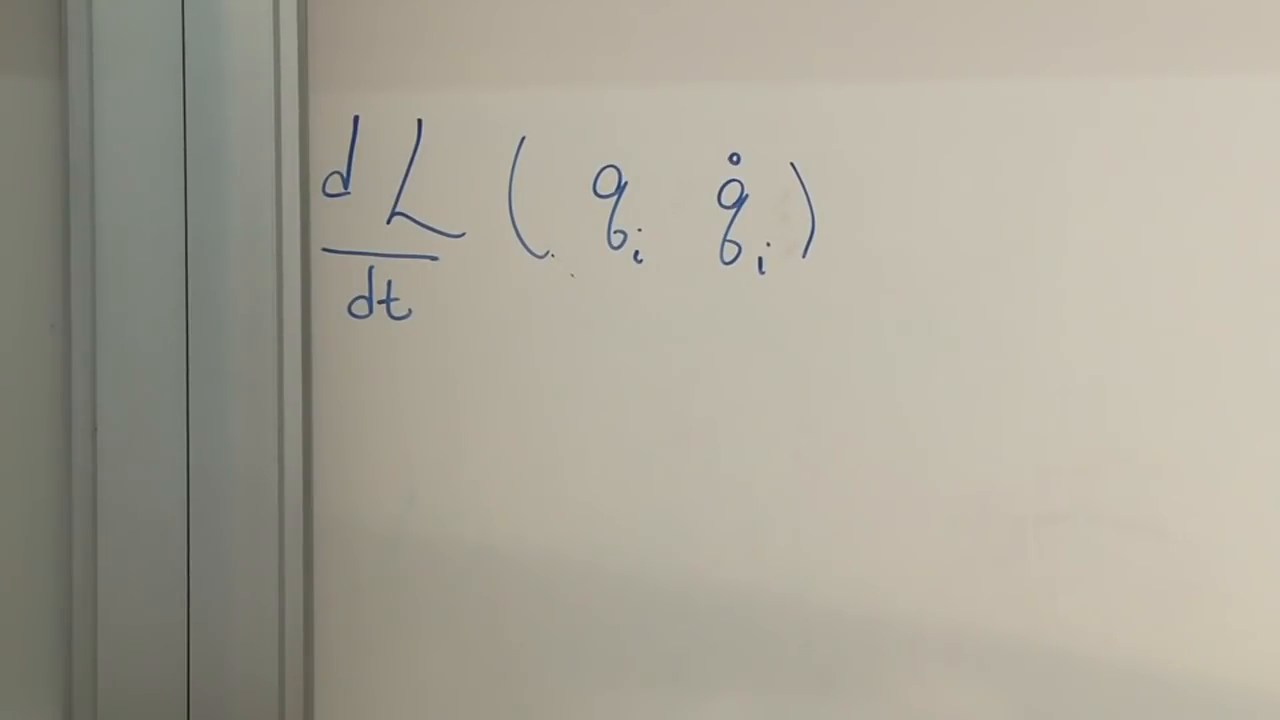
\includegraphics[width=0.72\textwidth]{lecture_05_figure_02.png}
  \caption{궤적을 따라 \(L(q_i,\dot q_i)\)를 미분하기 시작한다.}
  \lectureframe{01:08:51}
\end{figure}

\begin{classroomqa}
  \audiencequestion{연쇄법칙을 쓴 식에서 합 기호가 빠진 것 아닌가요?
  \lecturetimestamp{01:10:39--01:11:05}}
  \lecturerresponse{그렇다. 각 좌표와 각 속도가 라그랑지안을 바꿀 수 있으므로 두 항 모두 \(i\)에 대해 합해야 한다.}
\end{classroomqa}

정준 운동량과 오일러--라그랑주 방정식을 쓰면,
\begin{equation}
  p_i=\frac{\partial L}{\partial\dot q_i},
  \qquad
  \dot p_i=\frac{\partial L}{\partial q_i}.
  \label{eq:l5-p-and-pdot}
\end{equation}
식~\eqref{eq:l5-chain-rule-no-time}은 다음과 같이 된다.
\begin{align}
  \frac{dL}{dt}
  &=\sum_i(\dot p_i\dot q_i+p_i\ddot q_i)
  \notag\\
  &=\frac{d}{dt}\sum_i p_i\dot q_i.
  \label{eq:l5-product-rule}
\end{align}
여기서 ``마법''은 곱의 미분법일 뿐이다.

\begin{figure}[htbp]
  \centering
  \includegraphics[width=0.84\textwidth]{lecture_05_figure_21.png}
  \caption{운동 방정식을 이용해 연쇄법칙을 \(\sum_i p_i\dot q_i\)의 도함수로 바꾸었다.}
  \lectureframe{01:13:45}
\end{figure}

\begin{classroomqa}
  \audiencequestion{마지막 곱에서 \(q_i\)에는 점이 하나 붙나요, 둘 붙나요?
  \lecturetimestamp{01:14:31--01:15:32}}
  \lecturerresponse{곱 안에서는 점 하나가 붙은 \(p_i\dot q_i\)이다. 곱을 미분하면 \(\dot p_i\dot q_i+p_i\ddot q_i\)가 되므로, 전개된 두 번째 항에 점이 두 개 붙는 이유를 알 수 있다.}
\end{classroomqa}

두 도함수를 빼면 보존되는 조합을 얻는다. 관례에 따라 그 음수를 택해 해밀토니안이라고 부른다.
\begin{equation}
  H=\sum_i p_i\dot q_i-L.
  \label{eq:l5-hamiltonian-definition}
\end{equation}

\begin{figure}[htbp]
  \centering
  \includegraphics[width=0.80\textwidth]{lecture_05_figure_22.png}
  \caption{보존되는 조합 \(L-\sum_i p_i\dot q_i=-H\)과 해밀토니안의 정의.}
  \lectureframe{01:18:05}
\end{figure}

퍼텐셜 안의 입자 하나에 대해서는,
\begin{equation}
  L=\frac12m\dot x^2-V(x),
  \qquad p=m\dot x.
  \label{eq:l5-particle-lagrangian}
\end{equation}
따라서
\begin{align}
  H&=p\dot x-L
  \notag\\
   &=m\dot x^2-\left(\frac12m\dot x^2-V(x)\right)
  \notag\\
   &=\frac12m\dot x^2+V(x)=T+V.
  \label{eq:l5-particle-energy}
\end{align}

\begin{figure}[htbp]
  \centering
  \includegraphics[width=0.86\textwidth]{lecture_05_figure_23.png}
  \caption{퍼텐셜 안에 있는 입자의 해밀토니안은 익숙한 운동에너지와 퍼텐셜 에너지의 합으로 환원된다.}
  \lectureframe{01:20:50}
\end{figure}

이 유도 과정에서는 \(L\)의 특정한 형태를 가정하지 않았다. 따라서 이 형식론에서 에너지의 일반적인 정의는 \(T+V\)가 아니라 식~\eqref{eq:l5-hamiltonian-definition}이다.

\section{명시적 시간 의존성과 에너지 교환}

연쇄법칙에 명시적인 시간 의존성을 다시 포함하면,
\begin{equation}
  \frac{dL}{dt}
  =\sum_i\left(
    \frac{\partial L}{\partial q_i}\dot q_i
    +\frac{\partial L}{\partial\dot q_i}\ddot q_i
  \right)
  +\frac{\partial L}{\partial t}.
  \label{eq:l5-full-chain-rule}
\end{equation}
좌변은 운동을 따라 취한 전미분이다. 마지막 편미분은 \(q\)와 \(\dot q\)를 고정한 채 외부에서 변하는 매개변수만 미분한다. 같은 곱의 미분법을 적용하면 다음을 얻는다.
\begin{equation}
  \boxed{\frac{dH}{dt}=-\frac{\partial L}{\partial t}}.
  \label{eq:l5-hamiltonian-time}
\end{equation}

\begin{figure}[htbp]
  \centering
  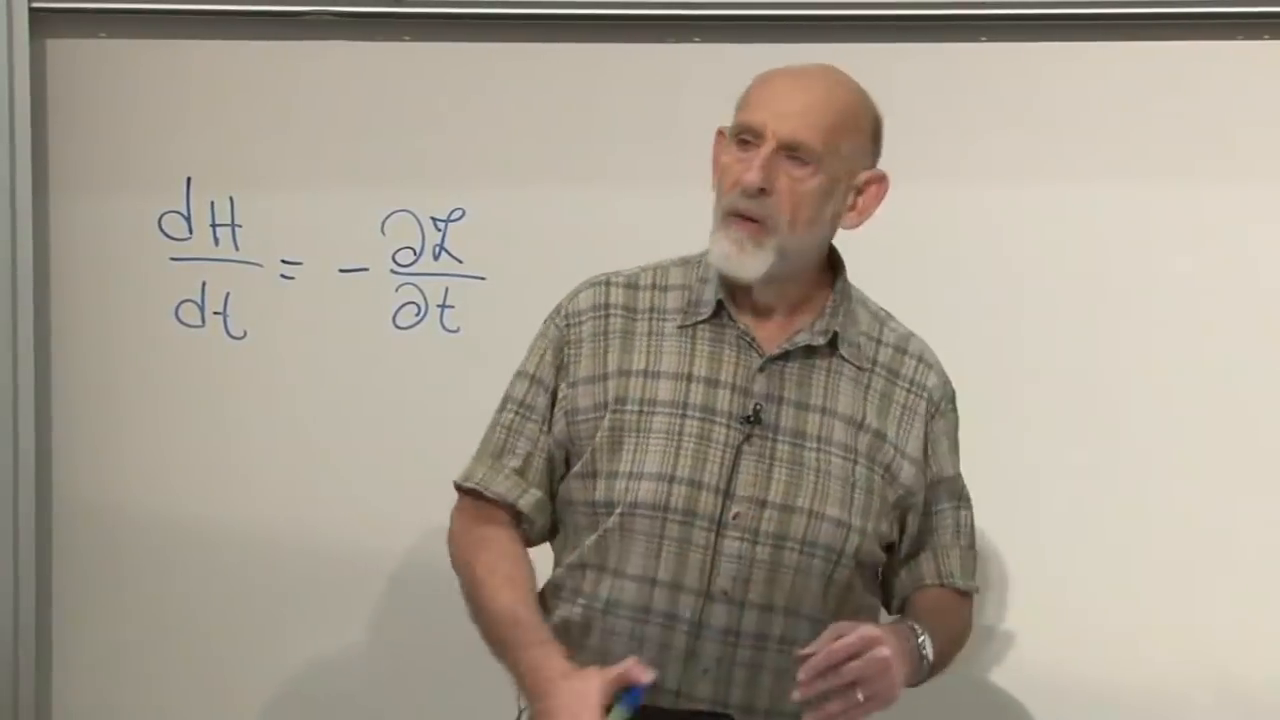
\includegraphics[width=0.70\textwidth]{lecture_05_figure_04.png}
  \caption{해밀토니안은 라그랑지안의 명시적 시간 의존성을 통해서만 변한다.}
  \lectureframe{01:37:22}
\end{figure}

식~\eqref{eq:l5-driven-oscillator}의 구동 조화 진동자에서는
\begin{equation}
  \frac{\partial L}{\partial t}
  =-\frac12\dot k(t)x^2,
  \qquad
  \dot H=\frac12\dot k(t)x^2.
  \label{eq:l5-driven-energy-rate}
\end{equation}
\(x=0\)에서는 순간 변화율이 사라진다. 원점에서 벗어나면 스프링 상수를 바꿀 때 \(x^2\dot k\)에 비례하는 비율로 일이 이루어진다.

\begin{classroomqa}
  \audiencequestion{에너지가 보존되지 않는다면 에너지는 해밀토니안의 시간 미분으로 정의되나요?
  \lecturetimestamp{01:27:11--01:28:04}}
  \lecturerresponse{아니다. 에너지는 \(H\)이다. 그 도함수는 에너지가 어떻게 변하는지를 알려 준다. 라그랑지안이 익숙한 형태이면 \(H=T+V\)이고, 그렇지 않으면 식~\eqref{eq:l5-hamiltonian-definition}이 정의를 준다. 외부 구동 장치를 포함하도록 계를 확장하면 전체 해밀토니안은 다시 보존된다.}
\end{classroomqa}

\begin{classroomqa}
  \audiencequestion{앞서 원심력과 코리올리 항이 등장한 회전 회전목마 위의 관찰자 문제에는 어떻게 적용되나요?
  \lecturetimestamp{01:28:08--01:29:52}}
  \lecturerresponse{일정하게 회전하는 좌표계는 시간에 따라 변하는 변수 변환이지, 고정된 공간 대칭도 단순한 시간 병진도 아니다. 변환된 라그랑지안으로 해밀토니안을 구성할 수 있지만, 대수 전개가 자기력 논의와 밀접하게 관련된 형태를 띠므로 그 별도 계산은 자기력을 다룰 때로 미루는 편이 낫다.}
\end{classroomqa}

\section{한눈에 보는 라그랑지안 도구}

이제 전체 구조를 간결하게 모아 쓰면 다음과 같다.
\begin{align}
  L&=L(q_i,\dot q_i,t),
  \notag\\
  p_i&=\frac{\partial L}{\partial\dot q_i},
  \qquad
  \dot p_i=\frac{\partial L}{\partial q_i},
  \notag\\
  \delta q_i&=\epsilon f_i(q)
  \quad\Longrightarrow\quad
  Q=\sum_i p_i f_i(q),\quad \dot Q=0,
  \notag\\
  H&=\sum_i p_i\dot q_i-L,
  \qquad
  \dot H=-\frac{\partial L}{\partial t}.
  \label{eq:l5-toolkit}
\end{align}

\begin{figure}[htbp]
  \centering
  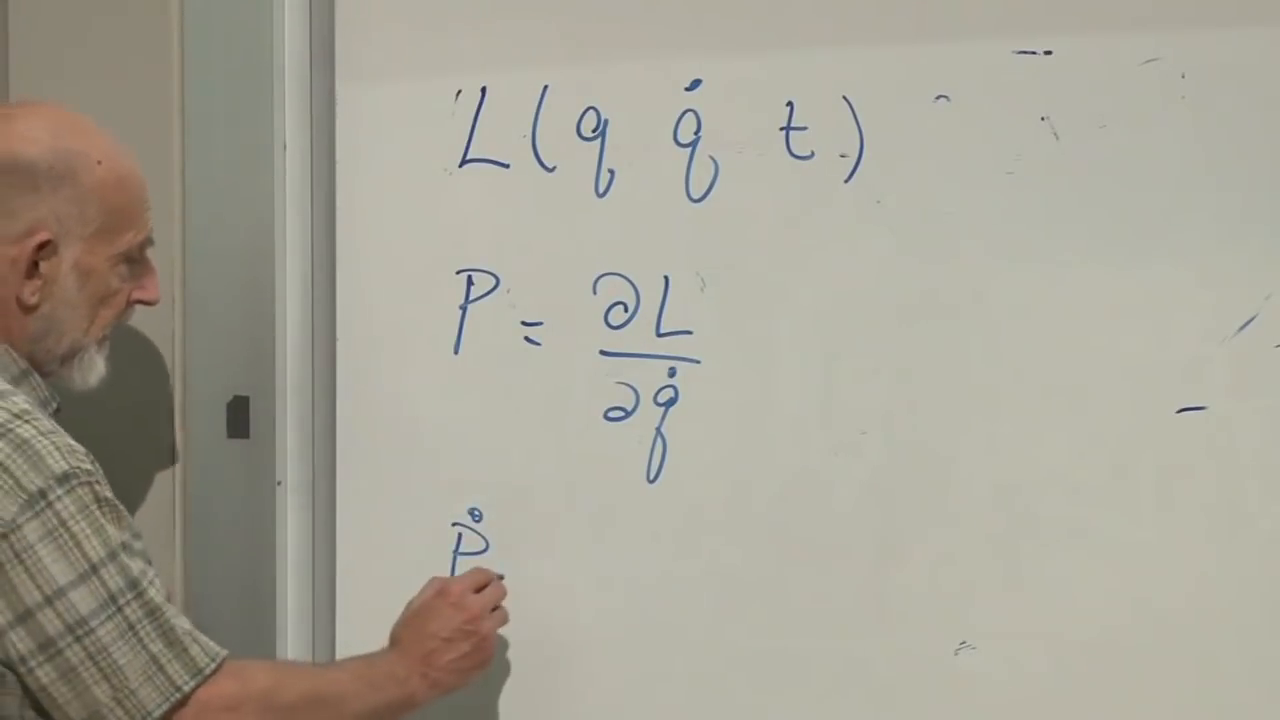
\includegraphics[width=0.66\textwidth]{lecture_05_figure_03.png}
  \caption{판서 요약은 \(L(q,\dot q,t)\), 정준 운동량, 오일러--라그랑주 방정식으로 시작한다.}
  \lectureframe{01:31:37}
\end{figure}

이 공식들에는 정의, 운동 방정식, 보통의 연속 대칭에 대응하는 전하, 시간 병진에 대응하는 전하가 담겨 있다. 특별한 요령은 많지 않다. 서로 무관한 식을 외우기보다 직접 다시 유도할 수 있는 것이 중요하다.

\section{라그랑지안 역학이나 해밀토니안 역학을 쓰는 이유}

\begin{classroomqa}
  \audiencequestion{역학은 \(L\)와 \(H\) 중 어느 쪽으로도 똑같이 기술할 수 있나요? 그렇다면 왜 한 형식을 선택하나요?
  \lecturetimestamp{01:37:16--01:39:18}}
  \lecturerresponse{르장드르 변환이 정칙이면 두 형식은 동등하지만, 강조하는 구조는 서로 다르다. 라그랑지안 형식은 정지작용 원리에서 자연스럽게 출발한다. 해밀토니안 역학은 처음에는 더 추상적이지만 방정식이 간결하고 양자역학에서 핵심적인 역할을 한다. 해밀토니안은 에너지이지만, 그 역할은 에너지 보존 법칙에만 국한되지 않는다.}
\end{classroomqa}

\begin{classroomqa}
  \audiencequestion{뉴턴은 해밀토니안 형식의 에너지 보존을 알고 있었나요?
  \lecturetimestamp{01:39:29--01:39:56}}
  \lecturerresponse{역사 기록이 보여 주는 한, 뉴턴은 이 형식으로 정식화하지 않았다. 뉴턴이 제시한 틀은 힘의 법칙 \(F=ma\)이었다.}
\end{classroomqa}

\begin{classroomqa}
  \audiencequestion{모든 물리계에 라그랑지안이 있어야 하는 이유는 무엇인가요? 그건 단지 실험적 사실인가요?
  \lecturetimestamp{01:39:57--01:42:37}}
  \lecturerresponse{여기서 다루는 폐쇄계의 경우 이는 경험적 사실이며, 더 근본적인 양자 기술에서도 따라 나온다. 수학적으로 일관되면서도 오일러--라그랑주 방정식이 아닌 미분방정식도 만들 수 있다. 예를 들어 \(\dot x=-x\)은 완전히 풀 수 있지만, 근본적인 폐쇄계의 1차원 법칙으로 보면 소산 현상처럼 정보를 잃는 성격을 가진다. 고전역학이 논리적으로 양자역학보다 앞서는 것은 아니다. 고전역학의 근본 구조는 양자역학에서 물려받는다. 자세한 이유는 뒤에서 다루겠다.}
\end{classroomqa}

\begin{classroomqa}
  \audiencequestion{실제 폐쇄계마다 라그랑지안이 있다면, 라그랑지안이라고 부르는 모든 함수가 자연에서 발견되는 계에 대응하나요?
  \lecturetimestamp{01:42:39--01:42:54}}
  \lecturerresponse{아니다. 형식적인 계산 체계에서는 알려진 어떤 물리계에서도 실현되지 않는 함수도 많이 허용한다.}
\end{classroomqa}

\begin{classroomqa}
  \audiencequestion{라그랑지안은 주로 퍼텐셜을 만들어 내는 도구인가요?
  \lecturetimestamp{01:42:54--01:43:32}}
  \lecturerresponse{그보다 쓰임이 넓다. 후보 역학계를 체계화할 수 있고, 운동 방정식을 얻는 가장 간결하고 실용적인 경로인 경우도 많다.}
\end{classroomqa}

이중진자는 그런 실용적 이점을 보여 준다. 두 각을 택하고, 그 각과 시간 미분으로 두 질량의 속도를 구해 \(T-V\)를 구성한 다음 오일러--라그랑주 방정식이 구속력을 암묵적으로 처리하게 한다. 모든 장력과 가속도를 \(F=ma\)로 하나하나 구하는 것보다 훨씬 간결하다.

\begin{figure}[htbp]
  \centering
  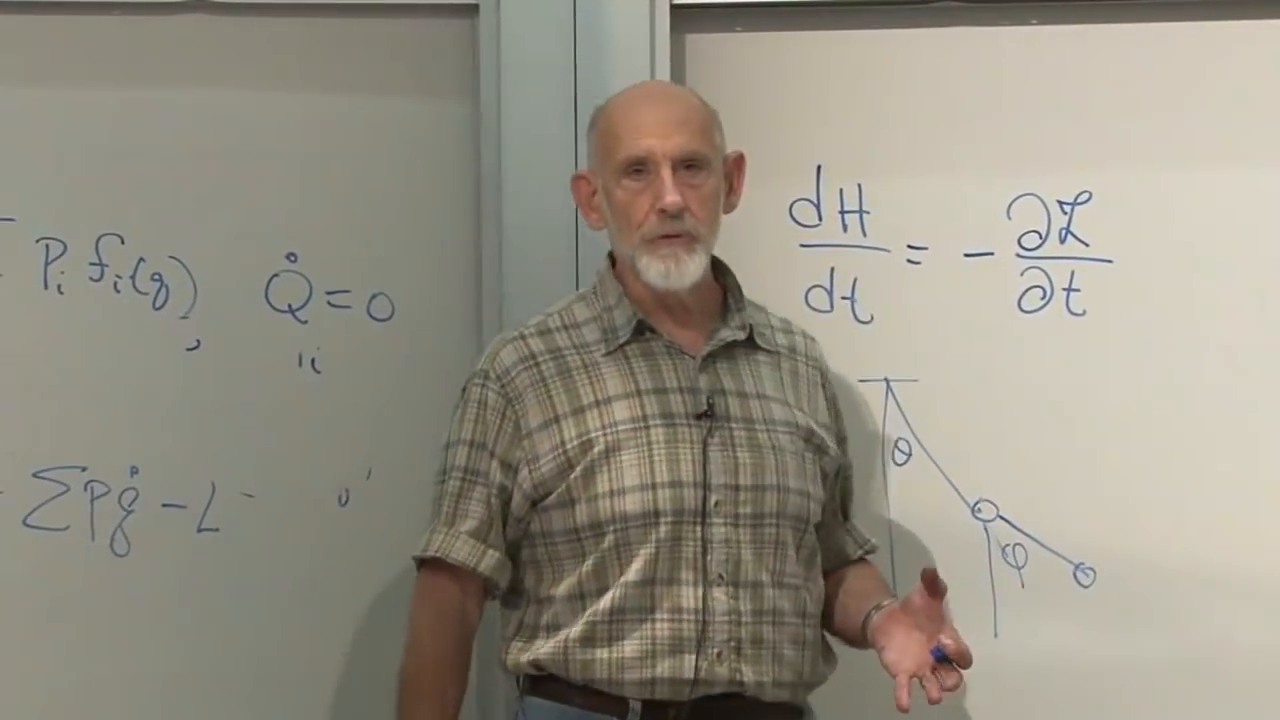
\includegraphics[width=0.84\textwidth]{lecture_05_figure_05.png}
  \caption{이중진자 그림 옆에는 에너지 변화율 항등식이 계속 남아 있다.}
  \lectureframe{01:45:39}
\end{figure}

\begin{figure}[htbp]
  \centering
  \begin{tikzpicture}[scale=1.15]
    \draw[thick] (-0.5,0) -- (0.5,0);
    \fill (0,0) circle (0.045);
    \draw[dashed] (0,0) -- (0,-2.3);
    \draw[thick] (0,0) -- (-0.92,-1.22);
    \fill (-0.92,-1.22) circle (0.07);
    \draw[dashed] (-0.92,-1.22) -- (-0.92,-2.55);
    \draw[thick] (-0.92,-1.22) -- (-0.25,-2.18);
    \fill (-0.25,-2.18) circle (0.07);
    \draw (0,-0.55) arc (-90:-127:0.55);
    \node at (-0.42,-0.56) {$\theta$};
    \draw (-0.92,-1.72) arc (-90:-55:0.48);
    \node at (-0.56,-1.72) {$\phi$};
  \end{tikzpicture}
  \caption{이중진자의 일반화된 각좌표.}
\end{figure}

변수 변환도 마찬가지로 효율적이다. 각각의 힘 방정식을 따로 변환하는 대신 라그랑지안 하나를 변환한 뒤 그에 대한 방정식을 유도하면 된다.

\begin{classroomqa}
  \audiencequestion{이중 진자는 태양, 지구, 달처럼 세 물체로 이루어진 또 다른 계에서 한 물체를 기준점으로 취급한 경우와 본질적으로 같은가요?
  \lecturetimestamp{01:45:06--01:45:25}}
  \lecturerresponse{그 비유는 계층 구조를 잘 포착하지만, 막대가 만드는 구속 조건은 다릅니다. 어느 경우든 질량이 매우 크거나 고정된 성분은 근사적으로 기준 구조로 취급할 수 있습니다.}
\end{classroomqa}

\begin{classroomqa}
  \audiencequestion{이중 진자에서는 \(T-V\)를 사용하지만, 방금 더 일반적인 라그랑지안도 강조하셨습니다. \(T-V\)는 언제 성립하나요?
  \lecturetimestamp{01:46:08--01:46:58}}
  \lecturerresponse{관성계에서 보는 보통의 비상대론적 입자에 자기장에 의한 속도 결합이 없을 때는 익숙한 형태가 적용됩니다. 회전 좌표계, 상대론적 계, 자기장이 있는 경우에는 더 일반적인 항이 필요합니다.}
\end{classroomqa}

\begin{classroomqa}
  \audiencequestion{충돌은 이 설명의 범위를 벗어나나요?
  \lecturetimestamp{01:47:00--01:48:05}}
  \lecturerresponse{탄성 충돌은 짧은 거리에서 작용하는 힘, 따라서 퍼텐셜에서 비롯됩니다. 비탄성 충돌도 미시적 수준에서는 역학적 현상이지만, 에너지는 내부 진동, 변형, 열로 들어갑니다. 이러한 자유도를 제외한 질량중심 기술은 불완전합니다.}
\end{classroomqa}

\begin{classroomqa}
  \audiencequestion{방망이에 맞은 야구공을 \(F=ma\)로 분석할 수 있나요?
  \lecturetimestamp{01:48:05--01:48:33}}
  \lecturerresponse{거친 수준에서만 가능합니다. 완전한 설명을 위해서는 변형, 가열, 공의 손상 가능성, 어쩌면 방망이가 부러지는 경우까지 다루어야 합니다. 현실적인 충돌이 점입자 충돌보다 훨씬 더 어려운 이유는 이런 내부 자유도에 있습니다.}
\end{classroomqa}

\begin{classroomqa}
  \audiencequestion{크기가 있는 강체는 어떤가요?
  \lecturetimestamp{01:48:34--01:49:00}}
  \lecturerresponse{강체는 뉴턴 역학의 방법으로 연구할 수도 있고, 병진 좌표와 회전 좌표로 쓴 \(T-V\) 라그랑지안으로 연구할 수도 있습니다. 그 라그랑지안을 구성하는 것은 유익한 연습입니다.}
\end{classroomqa}

\begin{classroomqa}
  \audiencequestion{양자역학의 에너지--시간 불확정성 관계는 에너지가 엄밀히 보존되지 않는다는 뜻인가요?
  \lecturetimestamp{01:49:01--01:49:29}}
  \lecturerresponse{아닙니다. 에너지는 엄밀히 보존될 수 있습니다. 이 관계가 말하는 것은 에너지를 높은 정확도로 알아내려면 오랜 시간 관측해야 한다는 점입니다. 이 관계가 보존 법칙을 대체하는 것은 아닙니다.}
\end{classroomqa}

\begin{classroomqa}
  \audiencequestion{뉴턴 역학과 라그랑주 역학은 논리적으로 동등한가요?
  \lecturetimestamp{01:49:36--01:50:07}}
  \lecturerresponse{두 정식화가 모두 적용되는 통상적인 영역에서는 동등합니다. 그렇더라도 기본적인 형태 \(m\ddot x=F(x)\)와 닮지 않은 운동 방정식을 주는 라그랑지안을 만들어낼 수는 있습니다.}
\end{classroomqa}

\section{좌표에 의존하는 운동에너지 항}

일부러 낯설게 만든 다음 예를 살펴봅시다.
\begin{equation}
  L=\frac12q^2\dot q^2-\frac12q^2.
  \label{eq:l5-nonstandard-l}
\end{equation}
이는 좌표에 의존하는 운동에너지 계수를 가진 유효한 라그랑지안입니다. \(q\dot q\)와 같이 속도에 선형인 항도 생각할 수 있습니다. 이 1차원 예에서 그 항은 전미분이므로 운동 방정식을 바꾸지 않습니다.

정준 운동량은 다음과 같습니다.
\begin{equation}
  p=\frac{\partial L}{\partial\dot q}=q^2\dot q,
  \label{eq:l5-nonstandard-p}
\end{equation}
따라서
\begin{equation}
  \dot p=q^2\ddot q+2q\dot q^2,
  \qquad
  \frac{\partial L}{\partial q}=q\dot q^2-q.
  \label{eq:l5-nonstandard-derivatives}
\end{equation}
운동 방정식은 다음과 같습니다.
\begin{equation}
  q^2\ddot q+q\dot q^2=-q.
  \label{eq:l5-nonstandard-eom}
\end{equation}

\begin{figure}[htbp]
  \centering
  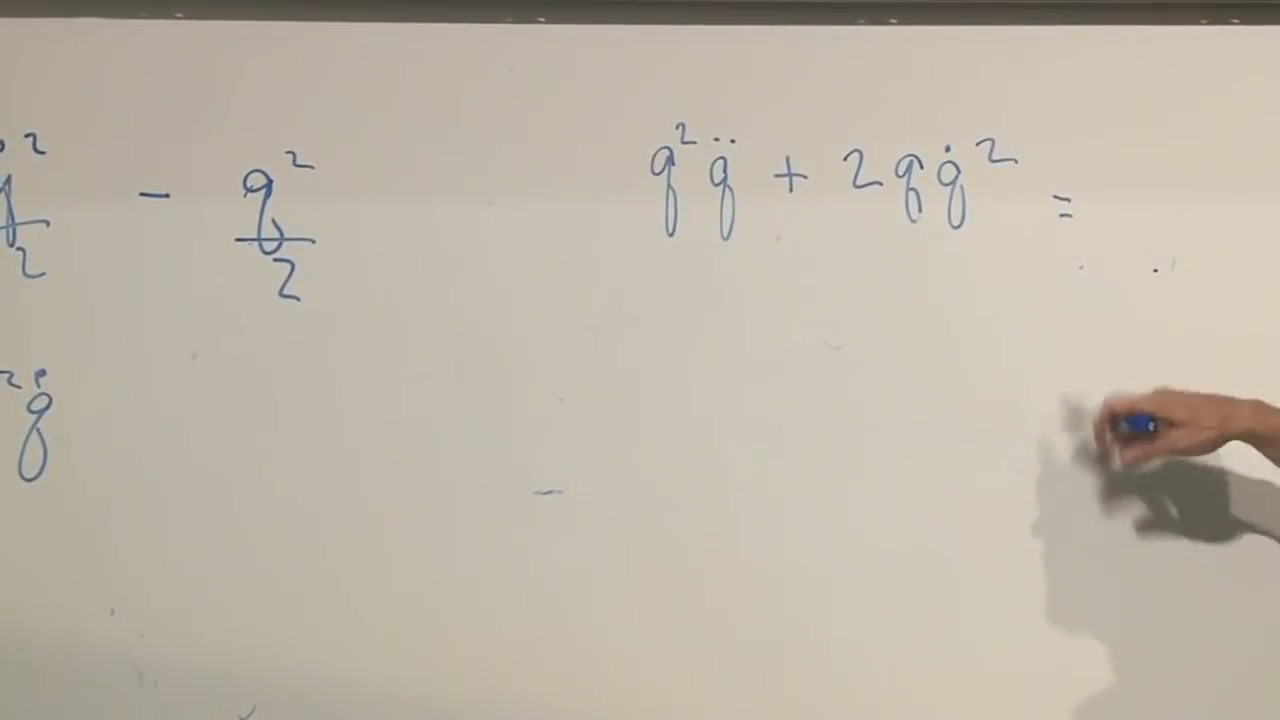
\includegraphics[width=0.80\textwidth]{lecture_05_figure_06.png}
  \caption{좌표 의존적 운동에너지 예에서 미분한 운동량.}
  \lectureframe{01:52:32}
\end{figure}

\begin{classroomqa}
  \audiencequestion{이 방정식을 \(q\)로 나누어도 되나요?
  \lecturetimestamp{01:53:22--01:53:39}}
  \lecturerresponse{\(q\neq0\)인 경우에만 가능합니다. \(q=0\)에서는 운동에너지 계수와 르장드르 사상이 퇴화하므로, 나누면 별도로 다뤄야 하는 특이점을 누락하게 됩니다.}
\end{classroomqa}

해밀토니안은 다음과 같습니다.
\begin{align}
  H&=p\dot q-L
  \notag\\
   &=q^2\dot q^2-
     \left(\frac12q^2\dot q^2-\frac12q^2\right)
  \notag\\
   &=\frac12q^2\dot q^2+\frac12q^2.
  \label{eq:l5-nonstandard-h}
\end{align}

\begin{classroomqa}
  \audiencequestion{그래도 \(q^2\dot q^2/2\)를 운동에너지라고 부를 수 있나요?
  \lecturetimestamp{01:54:41--01:55:07}}
  \lecturerresponse{네. 이 계산 예에서 해밀토니안은 다시 양의 운동에너지 항과 퍼텐셜 항의 합처럼 보입니다. 여기서 중요한 점은 기본적인 상수 질량 형태를 먼저 가정하지 않아도 형식적 정의가 작동했다는 것입니다.}
\end{classroomqa}

\section{소산과 형식의 더 깊은 기원}

\begin{classroomqa}
  \audiencequestion{마찰은 라그랑지안에 어떻게 포함하나요?
  \lecturetimestamp{01:55:09--01:56:17}}
  \lecturerresponse{여기서 다루는 단순한 폐쇄계, 즉 자유도가 유한한 계에서는 마찰을 근본적인 힘으로 포함하지 않습니다. 거시적 마찰은 엄청나게 많은 미시적 자유도의 통계적 효과입니다. 그 원자가 여전히 기저 역학을 따르지만, 원자를 추적하지 않는 축약된 기술에서는 소산이 나타납니다.}
\end{classroomqa}

\begin{classroomqa}
  \audiencequestion{해밀턴은 어떻게 자신의 정식화에 이르렀나요?
  \lecturetimestamp{01:56:22--01:56:37}}
  \lecturerresponse{여기서는 역사적 유도를 제시하지 않았습니다. 이 강의에서 중요한 과제는 그 정식화가 어떻게 작동하는지 이해하는 것입니다.}
\end{classroomqa}

\begin{classroomqa}
  \audiencequestion{라그랑지안이 눈에 띄게 \(T-V\) 형태가 아닐 때, 이를 구하는 더 일반적인 방법이 있나요?
  \lecturetimestamp{01:56:43--01:58:54}}
  \lecturerresponse{실험, 근거 있는 추측, 대칭 원리, 또는 원하는 방정식으로부터의 재구성을 통해 함수를 정할 수 있습니다. 미적분학 자체에 그 입력이 어디서 오는지 묻는 것은 도함수의 정의에 \(f(x)\)가 어디서 왔는지 묻는 것과 같습니다. 함수가 주어진 뒤에 무엇을 해야 하는지는 미적분학이 알려줍니다. 자연의 폐쇄계가 왜 이 추상적 구조를 따르는지는 양자역학이 더 깊은 수준에서 답합니다.}
\end{classroomqa}

이 점은 강의의 도입부에서 다룬 주제와 연결됩니다. 근본적인 해밀토니안 시간 변화는 궤적이 서로 합쳐지지 않고 정보가 단순히 소멸하지 않는다는 의미에서 결정론적이고 가역적입니다. 이 성질과 위상 공간 정식화의 관계는 단계적으로 전개할 것입니다.

\begin{classroomqa}
  \audiencequestion{변분법은 원하는 고전 방정식에서 역으로 거슬러 올라가 작동했을 뿐인가요? 양자역학도 같은 방식으로 라그랑지안을 얻나요?
  \lecturetimestamp{01:59:37--02:01:07}}
  \lecturerresponse{기초적인 고전역학의 구성에서는 알려진 방정식을 정지 경로로 재현하는 작용을 실제로 선택할 수 있습니다. 양자역학에서는 논리적 순서가 다릅니다. 양자역학은 자연스럽게 해밀토니안에서 출발해 라그랑지안 기술로 나아갈 수 있습니다. 고전역학에서 해밀토니안은 처음에는 추상적으로 보이지만, 양자역학에서는 더 직관적입니다.}
\end{classroomqa}

\begin{classroomqa}
  \audiencequestion{양자역학으로 마찰을 기술할 수 있나요?
  \lecturetimestamp{02:01:08--02:02:05}}
  \lecturerresponse{네. 다만 근본적인 기술에는 환경의 자유도를 포함해야 합니다. 점성이 있는 유체 속에서 움직이는 입자를 완전히 기술하려면 유체를 이루는 입자들도 고려해야 합니다. 마찰은 그 자유도를 하나씩 추적하지 않을 때 나타나는 복잡한 집단 효과입니다.}
\end{classroomqa}
\chapter{구속계와 해밀턴 운동}

\lectureoverview{두 가지 구속계는 라그랑주 역학이 왜 그토록 효과적인지를 보여 준다. 적절한 좌표를 선택하면 구속력을 명시적으로 계산하지 않고도 운동 방정식과 보존 법칙을 얻을 수 있다. 이어지는 같은 예제들은 해밀턴 역학으로 나아간다. 해밀턴 역학에서는 좌표와 운동량이 위상공간을 이루고, 조화 진동자는 강체 회전으로 나타나며, 2계 오일러--라그랑주 방정식은 해밀턴의 두 1계 방정식으로 대체된다.}

\section{역학 문제를 푼다는 것의 의미}

라그랑주 방법의 직접적인 목적은 실용적인 데 있다. 바닥 위를 미끄러지는 쐐기와 이중 진자는 모두 뉴턴 법칙으로 다룰 수 있지만, 미지의 접촉력과 장력을 일일이 계산하다 보면 금세 번거로워진다. 라그랑주 역학의 규칙을 알고 나면 같은 문제를 다음과 같이 단계적으로 다룰 수 있다:
\begin{enumerate}
  \item 순간적인 배치를 나타내는 독립 좌표를 선택한다;
  \item 그 좌표로 운동 에너지와 퍼텐셜 에너지를 표현한다;
  \item \(L=T-V\)를 구성하고 오일러--라그랑주 방정식을 적용한다.
\end{enumerate}

현재의 목적에서는 운동 방정식을 올바르게 세웠을 때 이미 문제를 \emph{풀었다}고 본다. 닫힌 형태의 궤적을 구하고 싶을 수도 있지만, 그것은 별개의 문제다. 역학적 설정을 마치고 나면 비선형 미분 방정식은 수치적으로 적분할 수 있다. 어려운 부분은 흔히 적분이 아니라, 불필요한 미지의 힘을 도입하지 않고 구속 조건을 반영하는 변수를 찾는 일이다.

\section{움직이는 쐐기 위를 미끄러지는 입자}

질량이 \(M\)인 쐐기가 마찰 없이 수평면을 따라 미끄러지도록 구속되어 있다고 하자. 질량이 \(m\)인 점입자는 경사면 위에 머물도록 구속되어 있다. 자유도는 두 개다. 하나는 쐐기의 위치를, 다른 하나는 쐐기 위에서 입자가 있는 위치를 나타낸다.

다음과 같이 두자.
\begin{equation}
  \begin{aligned}
    X&=\text{horizontal position of the wedge corner},\\
    x&=\text{horizontal displacement of the particle}\\[-0.2em]
     &\phantom{={}}\text{from that corner}.
  \end{aligned}
  \label{eq:l6-wedge-coordinates}
\end{equation}
따라서 입자의 절대 수평 좌표는 \(X+x\)이다. 좌표 선택은 하나로 정해져 있지 않다. 경사면을 따라 잰 거리나 입자의 절대 수평 좌표를 사용할 수도 있다. 같은 배치를 나타내는 비중복 좌표 쌍이라면 무엇이든 쓸 수 있지만, 어떤 쌍은 다른 쌍보다 계의 구조를 더 분명하게 드러낸다.

경사각 \(\beta\)이 고정되어 있으면 수직 변위 \(y\)는 독립적인 좌표가 아니다:
\begin{equation}
  y=x\tan\beta,
  \qquad
  \dot y=\dot x\tan\beta.
  \label{eq:l6-wedge-constraint}
\end{equation}
이제 \(\beta=45^\circ\)인 경우로 한정하면 \(y=x\)이고
\(\dot y=\dot x\)이다.  이 단순화는 예제의 요점을 바꾸지 않으면서 삼각함수 인자를 없앤다.

\begin{figure}[htbp]
  \centering
  \includegraphics[width=0.84\textwidth]{lecture_06_figure_06.png}
  \caption{\(45^\circ\) 예제에서 사용한 움직이는 쐐기와 구속된 입자, 수평 및 수직 속도 성분.}
  \lectureframe{00:10:25}
\end{figure}

쐐기의 운동 에너지는 다음과 같다.
\begin{equation}
  T_{M}=\frac{M}{2}\dot X^2.
  \label{eq:l6-wedge-kinetic}
\end{equation}
입자의 수평 속도는 \(\dot X+\dot x\)이고 수직 속도는 \(\dot x\)이다. 따라서 입자의 운동 에너지는
\begin{equation}
  T_m=\frac{m}{2}\left[(\dot X+\dot x)^2+\dot x^2\right].
  \label{eq:l6-particle-kinetic}
\end{equation}
중력 퍼텐셜의 영점을 \(x=0\)에 두면 \(V=mgx\)이다. 그러므로
\begin{equation}
  L=\frac{M}{2}\dot X^2
    +\frac{m}{2}\left[(\dot X+\dot x)^2+\dot x^2\right]
    -mgx.
  \label{eq:l6-wedge-lagrangian}
\end{equation}

\begin{figure}[htbp]
  \centering
  \includegraphics[width=0.86\textwidth]{lecture_06_figure_07.png}
  \caption{쐐기의 기하와 \(V=mgx\), 그리고 칠판에 정리한 두 운동 에너지 항.}
  \lectureframe{00:14:15}
\end{figure}

\subsection{정준운동량은 라그랑지안으로 정의된다}

정준운동량은 입자 속도 하나를 보고 짐작하는 것이 아니라 라그랑지안으로 정의한다:
\begin{align}
  p_X&=\frac{\partial L}{\partial\dot X}
      =M\dot X+m(\dot X+\dot x),
      \label{eq:l6-wedge-pX}\\
  p_x&=\frac{\partial L}{\partial\dot x}
      =m(\dot X+\dot x)+m\dot x.
      \label{eq:l6-wedge-px}
\end{align}
첫 번째 식은 보통의 전체 수평 운동량이다. 쐐기가 \(M\dot X\)만큼 기여하고, 입자가 \(m(\dot X+\dot x)\)만큼 기여한다. 이 운동량은 여기서 좌표 \(X\)에 켤레인 운동량으로 나타난다.

\begin{figure}[htbp]
  \centering
  \includegraphics[width=0.86\textwidth]{lecture_06_figure_08.png}
  \caption{쐐기 좌표 \(X\)와 입자의 상대 좌표 \(x\)에 켤레인 정준운동량.}
  \lectureframe{00:18:05}
\end{figure}

라그랑지안은 \(X\)에 명시적으로 의존하지 않는다. 장치 전체의 수평 병진 변환은 다음과 같이 작용한다.
\begin{equation}
  \delta X=\epsilon,
  \qquad
  \delta x=0.
  \label{eq:l6-wedge-translation}
\end{equation}
따라서 일반적인 무한소 대칭 규칙
\begin{equation}
  \delta q_i=\epsilon f_i(q),
  \qquad
  Q=\sum_i p_i f_i
  \label{eq:l6-noether-rule}
\end{equation}
에 따라 \(Q=p_X\)이다. 달리 말해 \(X\)는 순환 좌표이며,
\begin{equation}
  \dot p_X=\frac{\partial L}{\partial X}=0.
  \label{eq:l6-wedge-conservation}
\end{equation}

이에 대응하는 수직 병진 대칭은 없다. 쐐기는 수직으로 움직일 수 없고, 입자의 높이가 바뀌면 중력 퍼텐셜도 바뀐다. 수평 운동량은 보존되지만, 이 구속된 계의 수직 운동량은 보존되지 않는다.

상대 좌표에 대한 오일러--라그랑주 방정식은 다음과 같다.
\begin{equation}
  \dot p_x=\frac{\partial L}{\partial x}=-mg.
  \label{eq:l6-wedge-force}
\end{equation}
이 식은 칠판에서 부호를 바로잡아야 했다. 믿을 수 있는 방법은 \(L=T-V\)에서 시작하는 것이다. \(V=mgx\)이므로 라그랑지안의 미분은 \(-mg\)이다. \(x\)를 수평 변위로 도입했더라도 그 방정식에서 중력이 사라지는 것은 아니다. 구속 조건이 그 수평 변위를 수직 높이 \(y=x\)와 연결하기 때문이다.

수직항력이나 반작용력은 등장하지 않는다. 이런 힘은 구속 조건을 유지하는 데 필요한 만큼 작용한다. 뉴턴 방법에서는 이 힘들을 도입해 가속도와 함께 구해야 하지만, 일반화 좌표를 사용하면 그럴 필요가 없다.

\section{이중 진자와 좌표 선택의 묘미}

이제 질량이 각각 단위 질량인 두 물체를 길이가 단위 길이인 질량 없는 막대 두 개에 매달아 보자.  첫 번째 막대는 아래쪽 수직선과 \(\theta\)의 각을 이룬다.  두 번째 자유도에는 두 가지 선택지가 있다. 두 번째 절대각 \(\phi\)를 사용하거나, 두 막대 사이의 상대각 \(\alpha\)을 사용할 수 있다.

상대각을 선택하는 편이 계의 구조를 더 잘 드러낸다. 잠시 중력을 끄자. 장치 전체를 강체 회전시키면 절대 방향은 바뀌지만 막대 사이의 각도는 변하지 않는다:
\begin{equation}
  \theta\longrightarrow\theta+\epsilon,
  \qquad
  \alpha\longrightarrow\alpha.
  \label{eq:l6-double-rotation}
\end{equation}
이 좌표를 선택하면 회전 대칭은 하나의 좌표에만 작용한다. 그렇다고 다른 좌표계가 틀린 것은 아니다. 이 선택에서는 대칭과 그에 따른 보존량을 더 쉽게 알아볼 수 있다.

\begin{figure}[htbp]
  \centering
  \includegraphics[width=0.76\textwidth]{lecture_06_figure_09.png}
  \caption{첫 번째 절대각이 \(\theta\)이고 두 번째 막대의 각도가 첫 번째 막대에 대한 상대각 \(\alpha\)인 이중 진자.}
  \lectureframe{00:29:20}
\end{figure}

운동 에너지를 구할 때는 계산을 위한 보조 수단으로 데카르트 좌표를 사용하자. 수직 좌표를 아래쪽 방향으로 재면 첫 번째 추의 위치는
\begin{equation}
  x_1=\sin\theta,
  \qquad
  y_1=\cos\theta,
  \label{eq:l6-bob-one-position}
\end{equation}
이므로
\begin{equation}
  \dot x_1=\dot\theta\cos\theta,
  \qquad
  \dot y_1=-\dot\theta\sin\theta,
  \qquad
  \dot x_1^2+\dot y_1^2=\dot\theta^2.
  \label{eq:l6-bob-one-velocity}
\end{equation}
두 번째 추의 위치는
\begin{align}
  x_2&=\sin\theta+\sin(\theta+\alpha),\\
  y_2&=\cos\theta+\cos(\theta+\alpha),
  \label{eq:l6-bob-two-position}
\end{align}
따라서 예를 들어
\begin{equation}
  \dot x_2=\dot\theta\cos\theta
  +(\dot\theta+\dot\alpha)\cos(\theta+\alpha),
  \label{eq:l6-bob-two-xvelocity}
\end{equation}
이며, \(\dot y_2\)에도 같은 방식의 식이 성립한다.

\begin{figure}[htbp]
  \centering
  \includegraphics[width=0.88\textwidth]{lecture_06_figure_10.png}
  \caption{두 추가 위치를 나타내는 보조 데카르트 좌표. 이 좌표는 속도를 계산하는 데 쓰이며 추가 자유도로 도입한 것은 아니다.}
  \lectureframe{00:35:25}
\end{figure}

두 운동 에너지를 더하면 다음과 같이 일관된 결과를 얻는다. 교차항은 다음 항등식에서 나온다.
\begin{equation*}
  \cos A\cos B+\sin A\sin B=\cos(A-B).
\end{equation*}
\begin{equation}
  T=\dot\theta^2
    +\frac12(\dot\theta+\dot\alpha)^2
    +\dot\theta(\dot\theta+\dot\alpha)\cos\alpha.
  \label{eq:l6-double-kinetic}
\end{equation}

\begin{classroomqa}
  \audiencequestion{이 식에는 두 추의 운동 에너지가 이미 모두 포함되어 있나요? 혹시 2분의 1 계수가 빠진 것은 아닌가요?
  \lecturetimestamp{00:38:06--00:38:27}}
  \lecturerresponse{두 추의 운동 에너지가 모두 포함되어 있습니다. 이 식은
  \(\tfrac12(\dot x_1^2+\dot y_1^2+\dot x_2^2+\dot y_2^2)\)에서 나옵니다.
  두 기여가 같아서 합하면 첫 번째 항 \(\dot\theta^2\)이 됩니다. 빠진 계수는 없습니다.}
\end{classroomqa}

중력이 없으면 \(L=T\)에는 \(\theta\)가 명시적으로 나타나지 않는다. 따라서
\begin{equation}
  \dot p_\theta=\frac{\partial L}{\partial\theta}=0,
  \label{eq:l6-double-angular-conservation}
\end{equation}
이고, \(p_\theta\)는 전체 각운동량이다. \(\theta\)가 나타나지 않는다는 말의 정확한 의미에 주목하자. \(\dot\theta\)는 분명히 나타나지만, 미분되지 않은 좌표 자체는 나타나지 않는다.

중력을 다시 켜면 전역 회전 대칭이 깨진다. 앞서 정한 수직 좌표의 아래쪽 방향 규약에 따라 영점을 편리하게 정하면
\begin{equation}
  V=-g(y_1+y_2)
   =-g\left[2\cos\theta+\cos(\theta+\alpha)\right].
  \label{eq:l6-double-potential}
\end{equation}
상수를 더해도 결과는 달라지지 않는다. 중요한 점은 이제 \(\theta\)가 식에 명시적으로 나타나므로 그에 켤레인 운동량이 더는 보존되지 않는다는 것이다. 라그랑지안이 시간에 명시적으로 의존하지 않으므로 에너지는 계속 보존된다.

\begin{classroomqa}
  \audiencequestion{칠판의
  \(\dot\theta-\dot\alpha\)는
  \(\dot\theta+\dot\alpha\)이어야 하나요?
  \lecturetimestamp{00:43:00--00:43:54}}
  \lecturerresponse{여기서 사용한 방향 규약에서는 플러스 부호가 맞습니다. 이는 식 ~\eqref{eq:l6-bob-two-position}의 규약이며 운동 에너지 식 ~\eqref{eq:l6-double-kinetic}에도 그대로 적용됩니다. 양의 방향을 \(\alpha\)의 정의에서 반대로 정하면 관련 부호도 바뀌지만, 그 경우에는 모든 항에서 일관되게 바꾸어야 합니다. 칠판에서는 두 규약이 뒤섞였습니다.}
\end{classroomqa}

\begin{figure}[htbp]
  \centering
  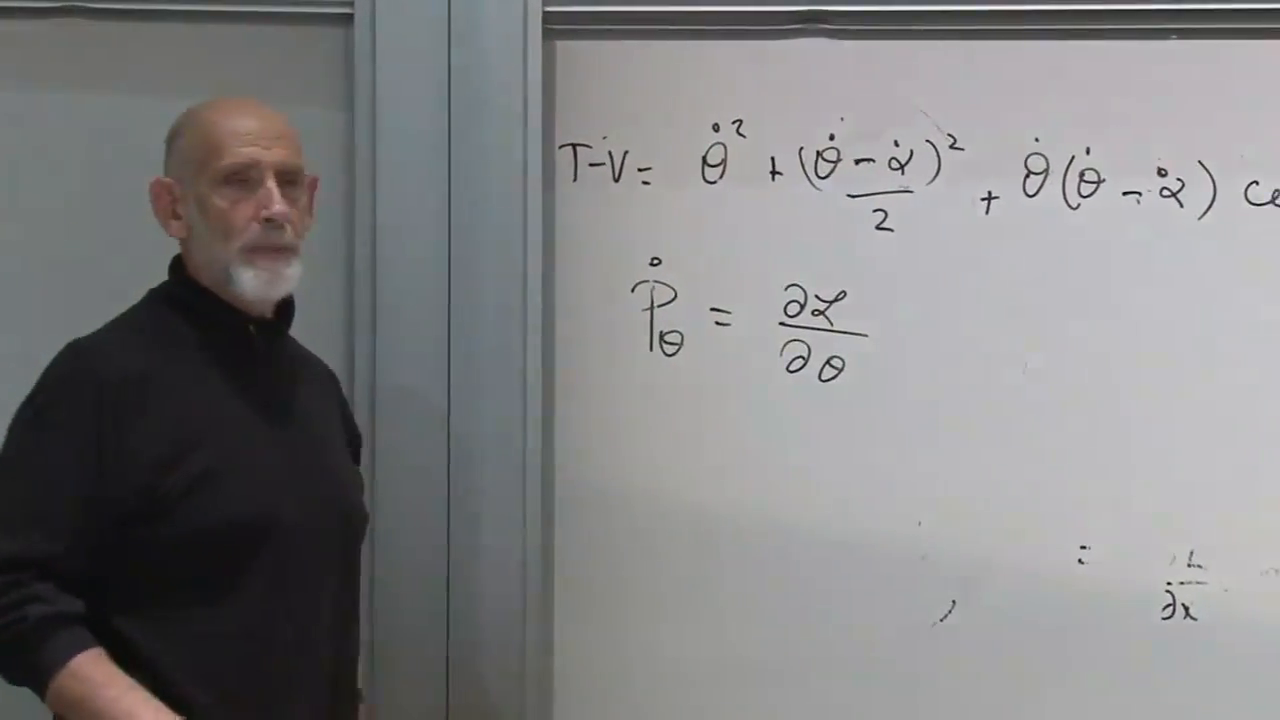
\includegraphics[width=0.84\textwidth]{lecture_06_figure_02.png}
  \caption{중력이 없는 이중 진자 계산과 \(\dot p_\theta=\partial L/\partial\theta\). 위쪽 칠판 식은 질문에서 다룬 부호 불일치가 있는 국소 표기를 그대로 보여 주며, 정규화된 식은 식 ~\eqref{eq:l6-double-kinetic}이다.}
  \lectureframe{00:45:50}
\end{figure}

\(T\)와 \(V\)를 알고 나면 나머지 방정식은 미분하여 얻을 수 있다. 막대의 장력과 고정된 길이를 유지하는 힘은 이번에도 좌표 선택에 흡수되어 나타나지 않는다.

\subsection{보존이 의미하는 것과 의미하지 않는 것}

\begin{classroomqa}
  \audiencequestion{방정식만 보고 이중 진자가 카오스적인지 직접 알 수 있나요?
  \lecturetimestamp{00:44:57--00:45:25}}
  \lecturerresponse{대개는 간단히 살펴보는 것만으로는 알기 어렵습니다. 매개변수나 에너지가 변하면 계의 거동이 규칙적 운동에서 카오스적 운동으로 바뀔 수 있습니다. 이 주제를 다루려면 방정식의 겉모습보다 더 많은 구조가 필요하며, 뒤에서 살펴보겠습니다.}
\end{classroomqa}

\begin{classroomqa}
  \audiencequestion{보존계에서는 모든 \(\dot p_i\)가
  영인가?
  \lecturetimestamp{00:45:25--00:46:24}}
  \lecturerresponse{아니다.  일반적인 방정식은
  \(\dot p_i=\partial L/\partial q_i\)이다.  \(q_i\)가 순환좌표일 때에만
  이 값은 영이 된다.  순환좌표는 다른 좌표들은 고정한 채 한 좌표만 이동시키는 대칭성이 주어진 특별히 단순한 경우다.}
\end{classroomqa}

목표가 수치적 시간 발전뿐이라면 불편한 좌표계를 써도 된다. 단지 방정식이 길어질 뿐이다. 좌표계를 잘 선택했을 때 얻는 이점은 개념적인 데 있다. 방정식을 풀기 전부터 보존 운동량을 알아볼 수 있다.

\begin{classroomqa}
  \audiencequestion{중력이 없으면 이중 진자는 하나의 자유 진자만큼
  단순하게 운동하는가?
  \lecturetimestamp{00:47:02--00:47:35}}
  \lecturerresponse{하나의 자유 로터는 각운동량 하나가 운동을 결정하므로
  등속 회전한다.  이중 진자는 전체 각운동량을 보존하면서도
  매우 복잡한 상대 운동을 할 수 있다.  처음에 두 각속도가 모두
  영이면 정지 상태를 유지하고, 그렇지 않으면 두 부분이 서로
  상호작용한다.}
\end{classroomqa}

\begin{classroomqa}
  \audiencequestion{중력이 없을 때 \(\dot\theta\)와 \(\dot\alpha\)는 각각 일정한가요?
  \lecturetimestamp{00:47:36--00:52:42}}
  \lecturerresponse{아닙니다. 보존 법칙은 \(\dot p_\theta=0\)라는 뜻이지, \(\ddot\theta=0\) 또는 \(\ddot\alpha=0\)라는 뜻은 아닙니다. \(p_\theta=\partial L/\partial\dot\theta\)의 식에는 두 각속도가 모두 들어가며 \(\alpha\)에도 의존합니다. 막대는 토크를 전달하여 두 추가 각운동량과 에너지를 주고받게 합니다. 이는 스프링으로 연결된 두 질점의 경우와 비슷합니다. 전체 운동량과 질량중심 속도는 일정하지만, 각 질점의 속도는 진동합니다. 회전에 대응하는 보존량은 두 각 가운데 어느 하나가 아니라 특정한 집단적 조합입니다.}
\end{classroomqa}

\begin{classroomqa}
  \audiencequestion{각운동량을 주고받게 하는 힘은 막대를 통해
  전달되는가?
  \lecturetimestamp{00:52:43--00:53:34}}
  \lecturerresponse{그렇다.  막대를 따라 전달되는 힘은 다른 운동의
  회전축을 지나지 않을 수 있으므로 토크를 가할 수 있다.  토크는
  힘이 일으키는 회전 경향일 뿐이며, 여기서는 각 부분에 영이 아닌
  각가속도를 만든다.}
\end{classroomqa}

\section{세 번째 정식화로서의 해밀턴 역학}

해밀토니안은 에너지이지만, 그것은 해밀토니안의 첫 번째 의미일 뿐이다. 해밀토니안은 역학의 세 번째 정식화의 토대이기도 하다. 뉴턴 방정식은 힘과 가속도를 사용한다. 정지 작용 원리는 오일러--라그랑주 방정식을 준다. 정칙계에서 해밀턴 역학은 후자와 동등하지만, 사용하는 변수와 기하학적 구조는 다르게 보인다.

\(q_i\)와 \(\dot q_i\) 대신 \(q_i\)와 그에 켤레인 운동량 \(p_i\)를 사용하자. 자유도가 \(n\)개인 계의 상태는 어느 표현에서든 \(2n\)개의 수로 나타낸다. 즉 위치와 속도 또는 위치와 운동량으로 나타낼 수 있다. 둘 사이의 연결은 다음과 같다.
\begin{equation}
  p_i=\frac{\partial L}{\partial\dot q_i}.
  \label{eq:l6-legendre-map}
\end{equation}
이 관계를 속도에 대해 풀 수 있다면
\(\dot q_i(q,p)\)해밀토니안을 다음과 같이 정의한다.
\begin{equation}
  H(q,p)=\sum_i p_i\dot q_i-L(q,\dot q).
  \label{eq:l6-hamiltonian-definition}
\end{equation}
그러면 우변의 속도를 없애고 \(q\)와 \(p\)만으로 표현할 수 있다. 이 가역성이 정칙 르장드르 변환의 가정이다. 특이 라그랑지안에는 더 일반적인 구속 조건 이론이 필요하므로, 이 기초적인 구성으로는 다루지 않는다.

\subsection{미적분에 앞서 되돌릴 수 있음 살펴보기}

화살표로 연결된 유한한 추상 상태 집합을 떠올려 보자. 결정론적 규칙이라도 이전 상태 둘이 하나의 나중 상태로 흘러들어 가면 되돌릴 수 없을 수 있다. 미래는 하나로 정해지지만 과거는 유일하지 않다. 화살표를 모두 뒤집으면 반대 문제가 생긴다. 하나의 상태에서 여러 미래가 갈라져 나온다. 첫 번째 그림에서는 화살표가 모이고, 두 번째 그림에서는 갈라진다.

\begin{figure}[htbp]
  \centering
  \includegraphics[width=0.86\textwidth]{lecture_06_figure_11.png}
  \caption{되돌릴 수 있는 순환과 허용되지 않는 수렴 및 발산을 대비하기 위한 추상 상태 사상.}
  \lectureframe{00:56:20}
\end{figure}

해밀턴 흐름은 이 진술을 연속적인 경우로 확장해 준다. 위상공간의 점들로 이루어진 구름은 움직이고 변형될 수 있지만, 상태 사이의 차이를 없애는 흡인점이나 하나의 상태에서 여러 미래를 만들어 내는 발산점은 생길 수 없다. 증명은 뒤로 미루고, 지금은 이 도식들을 통해 기하학적 관점을 살펴보자.

\begin{classroomqa}
  \audiencequestion{추상 상태 도식을 중력장에서 움직이는 물체로 해석해야 하나요?
  \lecturetimestamp{00:58:02--00:58:35}}
  \lecturerresponse{아닙니다. 점은 그저 추상적인 상태이고 화살표는 상태를 바꾸는 규칙을 나타냅니다. 이 그림에는 공간적 의미나 중력의 의미가 부여되어 있지 않습니다.}
\end{classroomqa}

\begin{classroomqa}
  \audiencequestion{허용되지 않는 수렴 상태 사상은 블랙홀과 어떻게 구별하나요?
  \lecturetimestamp{00:58:40--00:59:28}}
  \lecturerresponse{쉽지 않고, 미묘한 문제입니다. 타당한 질문이지만, 올바르게 답하려면 전체 상태와 그 양자 중력적 시간 발전을 세심하게 살펴야 합니다. 기초적인 도식만으로는 결론을 내릴 수 없습니다.}
\end{classroomqa}

\section{위상공간에 맞춘 진동자}

일반 방정식을 유도하기 전에, 위상공간에 맞게 의도적으로 표현한 조화 진동자를 살펴보자:
\begin{equation}
  L=\frac{1}{2\omega}\dot q^2-\frac{\omega}{2}q^2.
  \label{eq:l6-rescaled-lagrangian}
\end{equation}
켤레 운동량은 다음과 같다.
\begin{equation}
  p=\frac{\partial L}{\partial\dot q}=\frac{\dot q}{\omega},
  \qquad
  \dot q=\omega p.
  \label{eq:l6-rescaled-momentum}
\end{equation}
이를 식 ~\eqref{eq:l6-hamiltonian-definition}에 대입하면
\begin{align}
  H&=p\dot q-L\\
   &=\omega p^2-\frac{\omega p^2}{2}+\frac{\omega q^2}{2}
    =\frac{\omega}{2}(p^2+q^2).
  \label{eq:l6-oscillator-hamiltonian}
\end{align}

\begin{figure}[htbp]
  \centering
  \includegraphics[width=0.86\textwidth]{lecture_06_figure_12.png}
  \caption{위상공간에 맞춘 진동자의 르장드르 변환과 대칭적인 해밀토니안 \(H=\tfrac{\omega}{2}(p^2+q^2)\).}
  \lectureframe{01:08:20}
\end{figure}

\(q\)와 \(p\)로 이루어진 공간이 위상공간이다. 자유도가 하나이면 2차원 평면이고, 자유도가 둘이면 4차원 위상공간이다. 진동자의 에너지가 일정하면
\begin{equation}
  p^2+q^2=\frac{2H}{\omega},
  \label{eq:l6-energy-circle}
\end{equation}
궤적은 원 위에 머문다. 에너지 보존에 따라 운동은 그 원 가운데 하나에 제한된다.

\begin{figure}[htbp]
  \centering
  \includegraphics[width=0.82\textwidth]{lecture_06_figure_13.png}
  \caption{진동자의 위상평면에서 에너지가 일정한 동심원. 가로축은 \(q\), 세로축은 \(p\)이다.}
  \lectureframe{01:13:20}
\end{figure}

\section{해밀턴 방정식 유도}

유도 과정은 여러 변수의 함수에 대한 전미분을 다루는 연습이다. \(F(q,p)\)에 대해
\begin{equation}
  \delta F=\sum_i\left(
  \frac{\partial F}{\partial q_i}\delta q_i
  +\frac{\partial F}{\partial p_i}\delta p_i\right).
  \label{eq:l6-total-differential}
\end{equation}
계수는 어느 방향으로든 읽을 수 있다. \(\delta q_i\)의 계수는 \(\partial F/\partial q_i\)이고, \(\delta p_i\)의 계수는 \(\partial F/\partial p_i\)이다.

이제 \(H\)의 정의식을 변분하자:
\begin{align}
  \delta H
  &=\sum_i\left(\dot q_i\,\delta p_i
       +p_i\,\delta\dot q_i\right)-\delta L\\
  &=\sum_i\left(\dot q_i\,\delta p_i
       +p_i\,\delta\dot q_i
       -\frac{\partial L}{\partial q_i}\delta q_i
       -\frac{\partial L}{\partial\dot q_i}\delta\dot q_i\right).
  \label{eq:l6-vary-hamiltonian}
\end{align}
\(\partial L/\partial\dot q_i=p_i\)이므로 두 \(\delta\dot q_i\)항이 상쇄된다. 오일러--라그랑주 방정식에 따라 \(\partial L/\partial q_i=\dot p_i\)이므로, 남는 식은
\begin{equation}
  \delta H=\sum_i\left(\dot q_i\,\delta p_i
                     -\dot p_i\,\delta q_i\right).
  \label{eq:l6-reduced-variation}
\end{equation}

\begin{figure}[htbp]
  \centering
  \includegraphics[width=0.86\textwidth]{lecture_06_figure_14.png}
  \caption{\(\delta H\)를 전개한 곱의 미분식. \(p_i\,\delta\dot q_i\)항이 상쇄되기 전의 식이다.}
  \lectureframe{01:18:40}
\end{figure}

식 ~\eqref{eq:l6-reduced-variation}을 식 ~\eqref{eq:l6-total-differential}의 일반적인 전미분과 비교하면, 서로 독립인 계수로부터 해밀턴 방정식을 얻는다:
\begin{equation}
  \boxed{
  \dot q_i=\frac{\partial H}{\partial p_i},
  \qquad
  \dot p_i=-\frac{\partial H}{\partial q_i}.}
  \label{eq:l6-hamilton-equations}
\end{equation}

\begin{figure}[htbp]
  \centering
  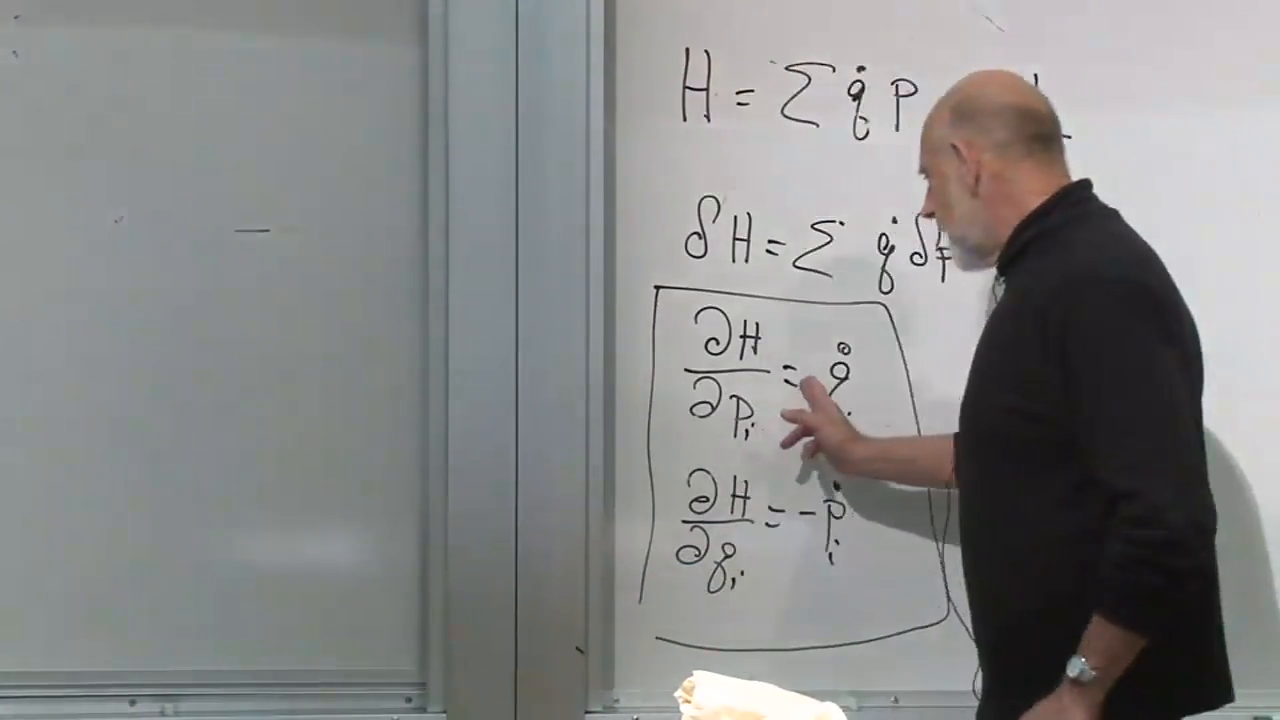
\includegraphics[width=0.78\textwidth]{lecture_06_figure_03.png}
  \caption{해밀토니안의 정의와 그 변분, 그리고 상자로 표시한 정준 방정식.}
  \lectureframe{01:22:18}
\end{figure}

\(n\)개의 좌표에 대해 이 식들은 1계 방정식 \(2n\)개를 이룬다. 반면 오일러--라그랑주 정식화는 2계 방정식 \(n\)개를 준다. 필요한 초기 조건의 양과 물리적 내용은 동일하다.

\section{진동자 운동은 강체 회전이다}

식 ~\eqref{eq:l6-hamilton-equations}을 식 ~\eqref{eq:l6-oscillator-hamiltonian}에 적용하면
\begin{equation}
  \dot q=\omega p,
  \qquad
  \dot p=-\omega q.
  \label{eq:l6-oscillator-first-order}
\end{equation}첫 번째 방정식을 미분하고 두 번째 방정식을 사용하면
\begin{equation}
  \ddot q=\omega\dot p=-\omega^2q.
  \label{eq:l6-oscillator-second-order}
\end{equation}따라서 두 1계 방정식은 운동량의 정의와 함께 보통의 2계 진동자 방정식을 정확히 재현한다.

위상공간에서 \((q,p)\)에 해당하는 속도 벡터는 \((\dot q,\dot p)=(\omega p,-\omega q)\)이며, 에너지 원에 접한다. 모든 반지름은 같은 각속도 \(\omega\)로 회전한다. 평면 전체를 강체 바람개비나 압축되지 않는 가상 유체로 생각할 수 있다. 점들은 순환하지만, 흡인점으로 모이거나 발산점에서 퍼져 나가지는 않는다.

\begin{figure}[htbp]
  \centering
  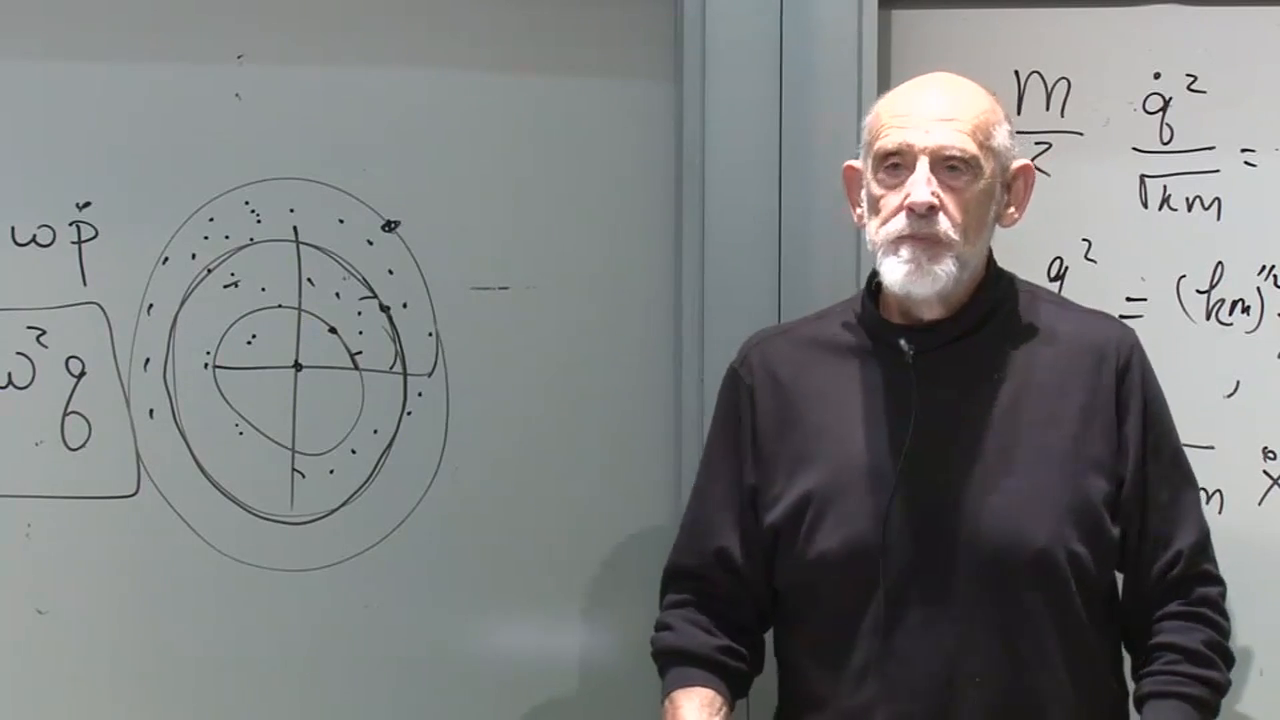
\includegraphics[width=0.86\textwidth]{lecture_06_figure_04.png}
  \caption{위상공간의 여러 궤적에 분포한 초기점들의 구름. 해밀턴 시간 발전은 구름을 선호되는 한 상태로 붕괴시키지 않고 구름 전체를 움직인다.}
  \lectureframe{01:39:27}
\end{figure}

\begin{figure}[htbp]
  \centering
  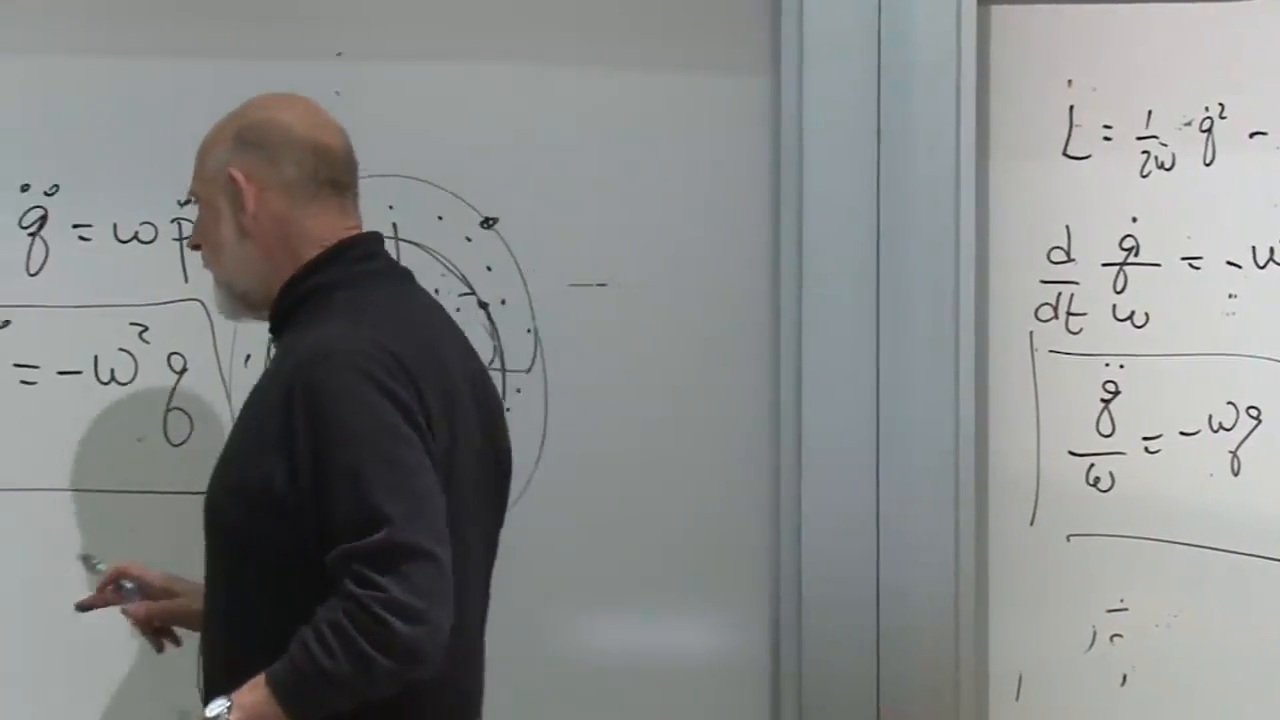
\includegraphics[width=0.90\textwidth]{lecture_06_figure_05.png}
  \caption{진동자의 위상도와 그에 동등한 오일러--라그랑주 방정식 \(\ddot q/\omega=-\omega q\).}
  \lectureframe{01:42:10}
\end{figure}

다음 단계에서는 유체 비유를 정리로 바꾸어, 해밀턴 흐름에는 국소적인 수렴이나 발산이 없음을 보일 것이다. 이 결과는 연속 역학을 강의 초반에 살펴본 가역 상태 사상과 다시 연결해 준다.

\section{좌표 선택의 의미를 드러내는 질문}

\begin{classroomqa}
  \audiencequestion{속도를 \(q\)와 \(p\)로 나타낼 수 있다는 가정은 정리인가요, 아니면 물리계의 경험적 성질인가요?
  \lecturetimestamp{01:29:08--01:29:45}}
  \lecturerresponse{이 기초적인 전개에서는 경험적으로 성립하는 규칙성으로 다루며, 양자역학에서 더 깊은 동기를 찾을 수 있습니다. 더 정확히 말하면 식 ~\eqref{eq:l6-legendre-map}의 속도에 대한 야코비안이 비특이행렬이어야 합니다. 현대 역학에는 중요한 특이 라그랑지안도 있으며, 특히 구속계와 게이지 계에서 나타납니다. 이런 계를 해밀턴 형식으로 다루려면 추가적인 구속 조건 형식이 필요합니다.}
\end{classroomqa}

단위에 관한 의문을 살펴보면 진동자를 식 ~\eqref{eq:l6-rescaled-lagrangian}의 익숙하지 않은 형태로 쓴 이유가 분명해진다. 먼저 보통 좌표 \(x\)에서 시작하자:
\begin{equation}
  L=\frac{m}{2}\dot x^2-\frac{k}{2}x^2,
  \qquad
  \omega=\sqrt{\frac{k}{m}}.
  \label{eq:l6-ordinary-oscillator}
\end{equation}
다음과 같이 두자.
\begin{equation}
  q=(km)^{1/4}x.
  \label{eq:l6-oscillator-rescaling}
\end{equation}
그러면 \(q^2=\sqrt{km}\,x^2\)이고
\(\dot q^2=\sqrt{km}\,\dot x^2\)이므로, 식 ~\eqref{eq:l6-ordinary-oscillator}은 정확히 식 ~\eqref{eq:l6-rescaled-lagrangian}으로 바뀐다. 새로운 \(q\)는 맞춤형 일반화 좌표이지 길이가 아니며, 그 켤레 \(p\)도 보통의 역학적 운동량 \(p_x=m\dot x\)가 아니다.

\begin{figure}[htbp]
  \centering
  \includegraphics[width=0.86\textwidth]{lecture_06_figure_15.png}
  \caption{보통의 진동자 좌표 \(x\)에서 맞춤형 좌표 \(q=(km)^{1/4}x\)로의 차원 재조정.}
  \lectureframe{01:36:10}
\end{figure}

\begin{classroomqa}
  \audiencequestion{\(\omega p=\dot q\)은 어떻게 차원적으로 일관되며, 왜 이 변수들을 선택했나요?
  \lecturetimestamp{01:29:46--01:39:22}}
  \lecturerresponse{\(q\)의 차원이 길이일 필요는 없고, 그 켤레 \(p\)의 차원도 \(m\dot x\)와 같을 필요는 없습니다. 식 ~\eqref{eq:l6-oscillator-rescaling}의 재조정은 라그랑지안의 차원을 보존하며 \(q\)와 \(p\)가 \(H\)에 대칭적으로 들어가게 합니다. 원래 변수로 쓰면
  \[
    H=\frac{p_x^2}{2m}+\frac{kx^2}{2},
  \]
따라서 \((x,p_x)\) 평면에서 에너지가 일정한 곡선은 타원입니다. 맞춤형 \((q,p)\) 평면에서는 원이 됩니다. 이러한 대칭이 드러나도록 재조정을 선택했습니다.}
\end{classroomqa}

\begin{classroomqa}
  \audiencequestion{\(2n\)개의 1계 해밀턴 방정식이 \(n\)개의 2계 라그랑주 방정식과 어떻게 동등할 수 있나요?
  \lecturetimestamp{01:39:24--01:42:30}}
  \lecturerresponse{진동자의 경우 \(\dot q=\omega p\)를 미분하고 \(\dot p=-\omega q\)를 대입하면 두 식은 \(\ddot q=-\omega^2q\)가 됩니다. 라그랑지안에서 바로 출발하면
  \[
    \frac{d}{dt}\left(\frac{\dot q}{\omega}\right)
      =-\omega q,
  \]
같은 2계 방정식을 얻습니다. 해밀턴 방정식 하나는 속도로부터 운동량을 정의하고, 다른 하나는 그 운동량의 시간 변화를 나타낸다고 볼 수 있습니다.}
\end{classroomqa}

\section{위상공간과 퍼텐셜 에너지가 중요한 이유}

\begin{classroomqa}
  \audiencequestion{해밀토니안의 유용성이 위상공간이 배치공간보다 더 나은 기하학적 표현임을 뜻하나요?
  \lecturetimestamp{01:42:33--01:44:38}}
  \lecturerresponse{두 공간은 서로 다른 목적에 쓰입니다. 위상공간에서는 순환 운동과 에너지 일정면, 그리고 수렴이나 발산의 부재가 특히 분명하게 드러납니다. 다른 문제에서는 배치공간이 더 유용할 수 있습니다. \(H\)를 강조하는 더 깊은 이유는 이것이 양자역학에서 핵심적이고 더 직관적인 대상이 되기 때문입니다. 양자역학은 이 역학 강의가 나아가는 현대 물리학의 주제 가운데 하나입니다.}
\end{classroomqa}

\begin{classroomqa}
  \audiencequestion{퍼텐셜 에너지를 힘의 적분으로 보아야 하나요?
  \lecturetimestamp{01:44:40--01:45:45}}
  \lecturerresponse{보존력이라면 상수항과 적절한 부호를 고려해 그 말이 맞습니다. 하지만 퍼텐셜을 기본량으로 두고 그로부터 일반화 힘을 구하는 편이 더 유용합니다:
  \[
    F_i=-\frac{\partial V}{\partial q_i}.
  \]
이는 \(\dot p_i=\partial L/\partial q_i\)에 나타나는 바로 그 항이며, 이때 \(L=T-V\)이고 운동 에너지는 \(q_i\)에 명시적으로 의존하지 않습니다.}
\end{classroomqa}

\begin{classroomqa}
  \audiencequestion{현대 물리학으로 이어지는 이 경로는 어떤 최전선의 문제를 밝히려는 것인가요?
  \lecturetimestamp{01:45:46--01:47:47}}
  \lecturerresponse{이 경로는 양자 중력과 우주론, 힉스 부문과 중성미자를 포함한 소립자 물리학, 상대론, 끈 이론, 양자장론으로 이어집니다. 이론 물리학의 지속적인 과제는 이 요소들을 하나의 일관된 구조로 통합하는 것입니다. 특히 양자역학과 중력, 우주론과 입자 물리학을 함께 설명하는 일이 그렇습니다. 이는 2011년에 바라본 최전선에 대한 설명이지, 그 문제가 이미 풀렸다는 주장은 아닙니다.}
\end{classroomqa}

이제 두 구속계 예제와 진동자를 하나의 그림으로 묶을 수 있다. 일반화 좌표는 불필요한 힘을 없앤다. 대칭은 보존되는 정준운동량을 골라낸다. 르장드르 변환은 속도를 운동량으로 바꾸고, 해밀턴 방정식은 동역학을 위상공간 위의 흐름으로 나타낸다. 진동자의 경우 그 흐름은 강체 회전이며, 일반적인 계에서는 그 기하학적 구조가 가역 운동의 연속적인 의미를 정확히 보여 줄 것이다.\chapter{리우빌 정리와 해밀턴 흐름}

\lectureoverview{해밀턴 방정식은 운동 방정식을 다른 형태로 다시 쓰는 데 그치지 않는다. 위상공간에서 발산이 영인 속도장을 정의한다. 이 단순한 상쇄가 바로 리우빌 정리다. 해밀턴 시간발전은 위상공간의 부피를 보존한다. 그 의미가 드러나는 순서대로 살펴보자---먼저 에너지 보존, 이어서 일정 에너지 곡면, 가능한 초기 조건들의 유체, 마지막으로 부피를 보존하는 흐름과 소산성 흡인점의 대비를 살펴본다. 같은 언어에서 푸아송 괄호도 자연스럽게 이어진다.}

\section{왜 또 다른 역학 형식인가?}

우리가 증명하려는 정리는 강의 초반에 도입한 가역 상태도에 대응하는 연속적인 고전역학의 정리다. 이산적인 가역 법칙에서는 모든 상태로 들어오는 화살표가 하나, 나가는 화살표가 하나씩 있다. 현재 상태만으로 다음 상태와 이전 상태를 모두 결정할 수 있다. 잘못된 법칙은 여러 상태를 하나의 흡인점으로 보낸다. 미래는 결정될 수 있어도 과거를 복원할 수는 없다.

리우빌 정리는 상태들의 집합이 연속 위상 공간일 때 이러한 구분이 어떻게 나타나는지 말해 준다. 들어오는 화살표 하나와 나가는 화살표 하나라는 표현은 \emph{유입량과 유출량이 같다}로 바뀐다. 하지만 이 표현을 수학적으로 만들려면 먼저 해밀턴 방정식에서 흐름을 재구성해야 한다.

그렇게 하다 보면 역사적인 수수께끼가 생긴다. 해밀턴, 야코비, 라그랑주, 푸아송은 자신들이 만든 정교하고 아름다운 고전역학의 형식이 필수적이 될 양자론을 알지 못한 채 이를 구축했다. 뉴턴에게는 행성 운동이라는 직접적인 목표가 있었다. 라그랑주와 해밀턴도 물리 문제를 다루었지만, 어느 한 궤도를 훨씬 넘어서는 유비와 구조를 탐구했다. 역학에서의 정상 작용 원리는 광학에서의 최소 시간 원리와 닮아 있었고, 광선의 운동과 입자의 운동은 평행한 수학적 형식으로 나타낼 수 있었다. 그들은 구조 자체에 물리학이 담겨 있는 듯했기 때문에 방정식을 단순화하고 재배열하고 통합했다.

오늘날 우리는 이러한 직관이 놀라울 만큼 생산적이었다는 것을 안다. 논리적으로는 고전역학의 많은 특징을 양자역학의 극한으로 이해할 수 있다. 하지만 역사적으로는 순서가 반대였다. 고전역학의 구조가 먼저 발견되었고, 그 더 깊은 쓰임은 훨씬 나중에야 분명해졌다. 파인먼에게 귀속되는 도발적인 농담은 내부 논리에 따라 추구되는 수학과, 외부의 동반자 즉 물리적 세계의 제약을 받는 물리학을 대비해 이 점을 짚었다. 그 농담은 논증은 아니지만, 여기서는 유용한 구분이다. 자연이 이 형식적 구조들을 거듭 선택하기 때문에 형식의 아름다움이 중요하다.

\begin{classroomqa}
  \audiencequestion{뉴턴은 오늘날의 운동에너지 개념을 갖고 있었을까? 에너지 개념은 어디서 시작되었을까?
  \lecturetimestamp{00:04:24--00:05:50}}
  \lecturerresponse{뉴턴 역학은 성숙한 일반 에너지 원리보다는 힘과 운동을 중심으로 구성되었다. 이 논의에서는 정확한 역사적 우선권이 확정되지 않는다. 라이프니츠의 \emph{비바 비스}, \(\sum_i m_i v_i^2\)는 중요한 선구 개념이었으며 현대적 운동에너지의 두 배에 해당한다. 이후 열에 관한 연구에서 열과 역학적 일 사이의 변환이 핵심이 되었다. 초기 열소 이론은 열을 보존되는 물질로 다루었으므로, 에너지의 여러 형태가 서로 변환될 수 있다는 현대적 관념은 점진적으로 형성되었다.}
\end{classroomqa}

\section{해밀턴 방정식과 에너지 보존}

계에 \(n\)개의 정준 좌표쌍이 있다고 하자.
\begin{equation}
  (q_i,p_i),\qquad i=1,\ldots,n.
  \label{eq:l7-canonical-pairs}
\end{equation}
각 좌표에는 운동량이 하나씩 대응하고, 각 운동량에는 좌표가 하나씩 대응한다. 운동 법칙은 하나의 함수로 표현된다.
\begin{equation}
  H=H(q_1,\ldots,q_n,p_1,\ldots,p_n,t),
  \label{eq:l7-hamiltonian}
\end{equation}
해밀턴 방정식은 다음과 같다.
\begin{equation}
  \boxed{
  \dot q_i=\frac{\partial H}{\partial p_i},
  \qquad
  \dot p_i=-\frac{\partial H}{\partial q_i}.}
  \label{eq:l7-hamilton-equations}
\end{equation}
부호는 정준 구조의 일부다. \(q\) 방정식에는 플러스 부호가, \(p\) 방정식에는 마이너스 부호가 붙는다.

\begin{figure}[htbp]
  \centering
  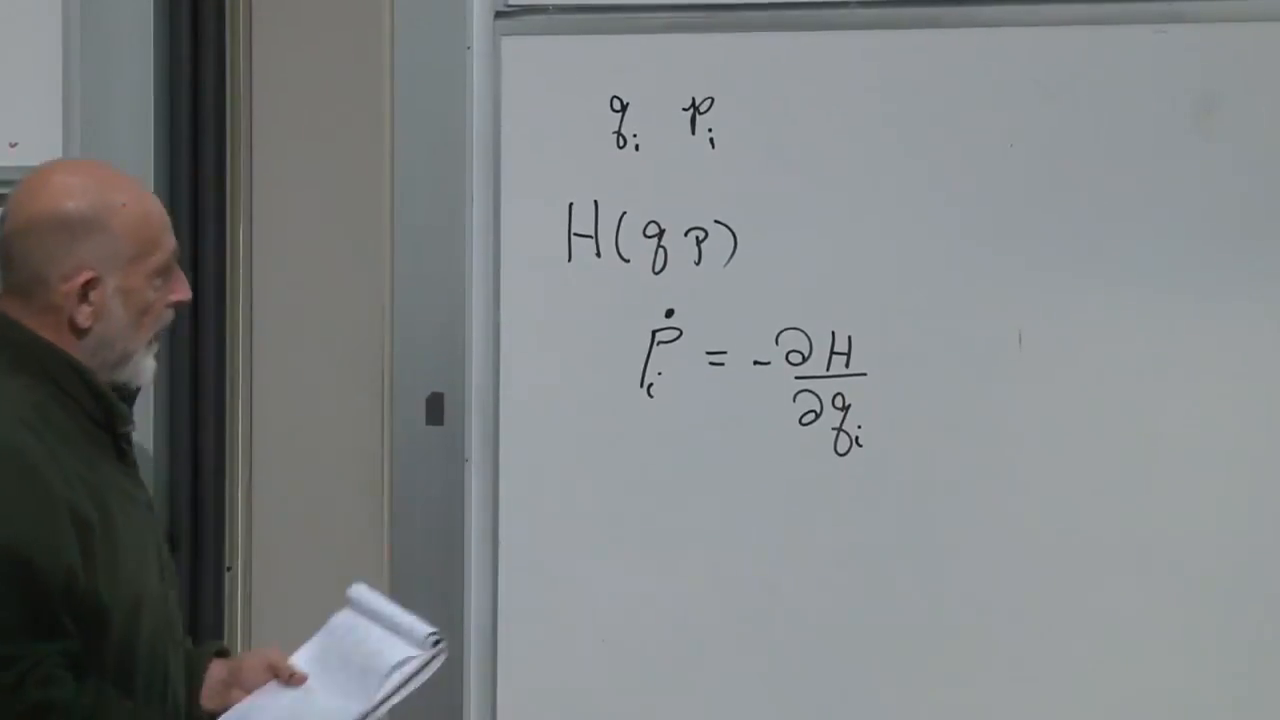
\includegraphics[width=0.82\textwidth]{lecture_07_figure_02.png}
  \caption{복습의 도입부에 제시된 정준변수와 함수 \(H(q,p)\), 그리고 운동량에 관한 해밀턴 방정식.}
  \lectureframe{00:07:29}
\end{figure}

방정식은 지표가 붙은 쌍으로 주어지지만, 운동이 쌍마다 분리될 필요는 없다. 해밀토니안은 모든 \(q_i\)와 \(p_i\)를 서로 결합할 수 있으므로, 예를 들어 \(\dot p_1\)는 계 전체의 상태에 의존할 수 있다.

\begin{classroomqa}
  \audiencequestion{이제 설명이 공리적이 되었나요? \(p\)와 \(q\) 사이의 어떤 관계를 가정했나요?
  \lecturetimestamp{00:17:08--00:18:18}}
  \lecturerresponse{\(H(q,p)\)와 정준 좌표쌍을 지정하면 해밀턴 방정식으로 형식 이론이 정의된다. 보편적으로 추가되는 가정 \(p=m\dot q\)은 없다. 이 관계는 운동에너지가 이차식인 보통의 데카르트 좌표계 입자에서는 성립하지만, 좌표나 해밀토니안이 달라지면 운동량--속도 관계도 달라진다. 그 관계는 방정식 자체에서 \(\dot q_i=\partial H/\partial p_i\)를 통해 주어진다. 제안된 해밀토니안이 자연에서 실현되는지는 별도의 물리적 문제다.}
\end{classroomqa}

이제 한 줄의 논리로 에너지 보존을 되짚어 볼 수 있다. 궤적을 따라 \(H\)의 전미분은 다음과 같다.
\begin{equation}
  \frac{dH}{dt}
  =
  \sum_i\left(
    \frac{\partial H}{\partial q_i}\dot q_i
    +\frac{\partial H}{\partial p_i}\dot p_i
  \right)
  +\frac{\partial H}{\partial t}.
  \label{eq:l7-total-h-derivative}
\end{equation}
마지막 항은 \(q\)와 \(p\)를 고정했을 때의 명시적 시간 의존성을 뜻한다. 외부에서 지정한 매개변수가 변하는 경우가 그 예다. 식~\eqref{eq:l7-hamilton-equations}을 대입하면,
\begin{align}
  \frac{dH}{dt}
  &=
  \sum_i\left[
    \frac{\partial H}{\partial q_i}
    \frac{\partial H}{\partial p_i}
    -\frac{\partial H}{\partial p_i}
    \frac{\partial H}{\partial q_i}
  \right]
  +\frac{\partial H}{\partial t}\\
  &=\frac{\partial H}{\partial t}.
  \label{eq:l7-h-energy-rate}
\end{align}
합의 각 항은 짝이 되는 항과 상쇄된다. 따라서
\begin{equation}
  \frac{\partial H}{\partial t}=0
  \quad\Longrightarrow\quad
  \frac{dH}{dt}=0.
  \label{eq:l7-energy-conservation}
\end{equation}
시간 병진 대칭성을 갖는 닫힌계에서는 해밀토니안이 보존되며, 이것이 에너지다.

\begin{classroomqa}
  \audiencequestion{해밀토니안이 시간에 명시적으로 의존하면 무엇이 달라지나요? \lecturetimestamp{00:10:32--00:12:33}}
  \lecturerresponse{그러면 식~\eqref{eq:l7-h-energy-rate}은 여전히 성립하지만, 부분계의 에너지는 일정하지 않을 수 있다. 명시적 시간 의존성은 대개 계와 에너지를 주고받는 외부 구동원이 생략되어 있음을 나타낸다. 그 구동원을 더 큰 닫힌계의 동역학적 일부로 포함하면, 더 큰 계의 해밀토니안은 다시 시간에 무관해질 수 있고 전체 에너지도 보존된다.}
\end{classroomqa}

\section{위상 공간의 기하로 보는 에너지}

이제 \(H\)가 시간에 명시적으로 의존하지 않는다고 하자. 초기 조건에 따라 값 \(E\)가 정해지고, 위상점은 \begin{equation}
  H(q,p)=E.
  \label{eq:l7-energy-surface}
\end{equation} 위에 머문다.
위상 공간의 차원은 \(2n\)이다. 정칙점에서는 좌표들 사이의 방정식 하나가 \((2n-1)\)차원 초곡면을 정의한다. \(E\)의 값이 다르면 서로 다른 초곡면이 주어진다. 이 초곡면이 닫혀 있거나 유계일 필요는 없다. 에너지 보존이 말해 주는 것은 그중 하나에서 시작한 궤적이 그 초곡면을 벗어나지 않는다는 것뿐이다.

앞 강의에서 다룬 조화진동자의 정준화된 형식에서는,
\begin{equation}
  H=\frac{\omega}{2}(p^2+q^2).
  \label{eq:l7-oscillator-hamiltonian}
\end{equation}
따라서 각 일정 에너지 집합은 원이다.
\begin{equation}
  p^2+q^2=\frac{2E}{\omega}.
  \label{eq:l7-oscillator-circle}
\end{equation}

\begin{figure}[htbp]
  \centering
  \includegraphics[width=0.84\textwidth]{lecture_07_figure_04.png}
  \caption{\(2n\)차원 위상공간 도식과 일정 에너지 곡면을 도입할 때 사용한 조화진동자의 해밀토니안.}
  \lectureframe{00:15:20}
\end{figure}

운동 방정식은
\begin{equation}
  \dot q=\omega p,\qquad \dot p=-\omega q,
  \label{eq:l7-oscillator-flow}
\end{equation}
위상점을 해당 원을 따라 시계 방향으로 움직인다. 에너지 방정식은 운동이 놓이는 곡선을 알려 주고, 해밀턴 방정식은 그 곡선을 따라가는 방향과 속력을 알려 준다.

\begin{figure}[htbp]
  \centering
  \begin{tikzpicture}[scale=0.95]
    \draw[->] (-2.7,0) -- (2.7,0) node[right] {\(q\)};
    \draw[->] (0,-2.7) -- (0,2.7) node[above] {\(p\)};
    \draw[thick] (0,0) circle (0.8);
    \draw[thick] (0,0) circle (1.5);
    \draw[thick] (0,0) circle (2.2);
    \draw[->,very thick] (0,2.2) arc[start angle=90,end angle=40,radius=2.2];
    \draw[->,very thick] (1.5,0) arc[start angle=0,end angle=-50,radius=1.5];
    \draw[->,very thick] (0,-0.8) arc[start angle=-90,end angle=-140,radius=0.8];
  \end{tikzpicture}
  \caption{일정한 에너지가 원들을 정하고, 진동자 방정식이 시계 방향 접선 흐름을 정한다.}
\end{figure}

\begin{classroomqa}
  \audiencequestion{해밀턴 방정식 두 개와 \(H=E\)는 같은 방정식을 달리 쓴 것인가요?
  \lecturetimestamp{00:15:53--00:17:06}}
  \lecturerresponse{아니다. 해밀턴 방정식은 정준 좌표쌍 하나에 대한 1계 운동 법칙 두 개다. 이 방정식들로부터 \(dH/dt=0\)가 나오고, 여기서 \(H=E\)가 따른다. \(E\)의 값은 초기 조건으로 정해진다. 방정식 \(H=E\)은 곡면을 지정할 뿐, 그 곡면을 따라가는 속도를 그 자체로 정하지는 않는다.}
\end{classroomqa}

\section{한 상태에서 상태들의 흐름으로}

초기 조건 하나를 따라가는 대신, 가능한 모든 초기 조건을 위상 공간에 뿌려 놓고 시간을 흘려 보자. 각 점은 완전한 가능한 상태 하나이며, 각 상태는 해밀턴 방정식에 따라 움직인다. 이 점들의 분포는 먼지나 가상의 유체로 상상할 수 있다. 실제 물질을 위상 공간에 쏟아붓는 것은 아니다. 이 유체는 모든 궤적을 한꺼번에 살펴보기 위한 표현이다.

위상 공간의 속도장은
\begin{equation}
  \mathbf V(q,p,t)
  =
  (\dot q_1,\ldots,\dot q_n,\dot p_1,\ldots,\dot p_n).
  \label{eq:l7-phase-velocity}
\end{equation}
정준 좌표쌍 하나에 대해서는 다음과 같이 쓴다.
\begin{equation}
  V_q=\dot q=\frac{\partial H}{\partial p},
  \qquad
  V_p=\dot p=-\frac{\partial H}{\partial q}.
  \label{eq:l7-phase-components}
\end{equation}
해밀토니안은 각 점에서 위상점을 다음에 어디로 보낼지 나타내는 벡터를 정한다. \(H\)가 시간에 무관하면 벡터장은 정상 상태다. 같은 위상점으로 돌아오면 같은 속도를 얻는다. \(H\)가 시간에 의존하면 벡터장 자체가 시간에 따라 변하지만, 그래도 매 순간 정의된다.

\begin{figure}[htbp]
  \centering
  \includegraphics[width=0.84\textwidth]{lecture_07_figure_05.png}
  \caption{조화진동자의 속도장. 벡터는 원에 접하며 원점에 가까울수록 짧아진다.}
  \lectureframe{00:24:50}
\end{figure}

조화진동자에서는 모든 반지름이 각속력 \(\omega\)로 회전한다. 원점에 가까운 점은 같은 주기 동안 더 짧은 원을 따라가므로 선속력이 더 작다. 따라서 먼지 전체는 강체 회전목마처럼 회전한다.

\begin{classroomqa}
  \audiencequestion{강체 회전이라면 모든 조화진동자 궤도의 주기가 같은가요? \lecturetimestamp{00:21:10--00:21:42}}
  \lecturerresponse{그렇다. 진폭과 무관하다는 점이 조화진동자를 특징짓는 특별한 성질이다. 위상 공간 속도 벡터의 크기는 작은 원일수록 작지만, 모든 원을 같은 각진동수 \(\omega\)로 돈다.}
\end{classroomqa}

\begin{classroomqa}
  \audiencequestion{위상 공간의 속도는 모든 점에서 같은가요?
  \lecturetimestamp{00:24:29--00:25:37}}
  \lecturerresponse{아니다. 방향과 크기는 일반적으로 위치에 따라 달라진다. 조화진동자에서 벡터는 그 점의 원에 접하며 크기는 \(\omega\sqrt{p^2+q^2}\)이다. 벡터장이란 모든 점에 각각 하나씩 벡터를 지정한 것이지, 똑같은 벡터 하나를 모든 곳에 복사한 것이 아니다.}
\end{classroomqa}

\begin{classroomqa}
  \audiencequestion{이 가상 유체의 입자와 밀도는 정확히 무엇을 뜻하나요? \lecturetimestamp{00:56:03--00:58:40}}
  \lecturerresponse{각 점은 역학계 전체의 완전한 상태 하나를 나타낸다. 물리적 입자 하나를 뜻하는 것이 아니다. 공간 차원이 1인 곳에서 입자 5개의 상태를 나타내려면 위치 5개와 운동량 5개가 필요하므로 위상 공간은 10차원이다. 3차원 공간에서는 30차원이 필요하다. 먼지는 서로 다른 대안적 상태들의 앙상블이다. 유체 그림이 오히려 혼란스럽다면 초기 조건 영역 하나를 잡아 그 안의 모든 점을 시간에 따라 진화시키고, 전후의 위상 공간 부피를 비교하면 된다.}
\end{classroomqa}

\section{압축과 발산}

이 가상 유체의 부피가 줄어드는지 알아보려면 1차원에서 시작하자. 직선 위의 점들이 속도 \(v(x)\)로 움직인다고 하자. \(\delta x\)만큼 떨어진 두 점 사이의 속도 차는
\begin{equation}
  \delta v \simeq \frac{dv}{dx}\,\delta x.
  \label{eq:l7-one-dimensional-strain}
\end{equation}
\(dv/dx>0\)이면 앞쪽 점이 더 빠르게 움직여 구간이 늘어난다. \(dv/dx<0\)이면 구간은 압축된다. 따라서 정상 1차원 비압축성 흐름은
\begin{equation}
  \frac{dv}{dx}=0.
  \label{eq:l7-one-dimensional-incompressible}
\end{equation}

\begin{figure}[htbp]
  \centering
  \includegraphics[width=0.84\textwidth]{lecture_07_figure_06.png}
  \caption{\(dv/dx\)를 국소적인 늘어남 또는 압축률로 도입하는 1차원 구성.}
  \lectureframe{00:30:20}
\end{figure}

서로 동등한 관점이 두 가지 있다. 물질 구간을 따라가며 길이가 변하는지 살펴볼 수 있다. 또는 작은 구간을 고정해 놓고 단위 시간당 들어오는 양과 나가는 양이 같은지 물을 수 있다. 첫 번째는 유체를 따라가고, 두 번째는 유체가 지나가는 모습을 관찰한다.

여러 차원에서는 전체 부피가 변하지 않으면서 한 축을 따라 영역이 늘어나고 다른 축을 따라 압축될 수 있다. 속도장 \(\mathbf V=(V_x,V_y,V_z)\)에 대해 관련된 국소 변화율은 발산이다.
\begin{equation}
  \nabla\cdot\mathbf V
  =
  \frac{\partial V_x}{\partial x}
  +\frac{\partial V_y}{\partial y}
  +\frac{\partial V_z}{\partial z}.
  \label{eq:l7-spatial-divergence}
\end{equation}
발산이 양수이면 국소적으로 팽창하고, 음수이면 국소적으로 수축하며, 비압축성 조건은
\begin{equation}
  \nabla\cdot\mathbf V=0.
  \label{eq:l7-zero-divergence}
\end{equation}
고정된 작은 상자를 드나드는 유량이 같은 것은 움직이는 작은 상자의 부피가 보존된다는 것과 동일한 국소적 진술이다.

\begin{figure}[htbp]
  \centering
  \includegraphics[width=0.86\textwidth]{lecture_07_figure_07.png}
  \caption{2차원 상자와 그 흐름 성분, 그리고 발산을 정의하는 동일 좌표에 대한 미분들의 합.}
  \lectureframe{00:35:30}
\end{figure}

\begin{classroomqa}
  \audiencequestion{보통 공간의 유체를 다루는 건가요, 위상 공간의 흐름을 다루는 건가요? \lecturetimestamp{00:34:27--00:34:40}}
  \lecturerresponse{발산 논증은 우선 일반적인 유체 논증이다. 이제 이를 차원이 짝수인 위상 공간에 적용할 것이다. 이 공간에서 좌표 방향은 \(q_i\)와 \(p_i\)이고 속도 성분은 \(\dot q_i\)와 \(\dot p_i\)이다.}
\end{classroomqa}

이제 이산 상태 사상으로 돌아가자. 가역 순환에서는 각 노드에 들어오는 화살표와 나가는 화살표가 하나씩 있으며, 선택한 상태들의 집합은 진화해도 원소 수를 그대로 유지한다. 흡인점에서는 들어오는 화살표가 많고 나가는 화살표는 너무 적다. 여러 대안이 서로 구분되지 않게 된다.

\begin{figure}[htbp]
  \centering
  \includegraphics[width=0.80\textwidth]{lecture_07_figure_08.png}
  \caption{발산 개념을 첫 강의의 가역 법칙 판별 기준과 다시 연결하는 이산 흡인점.}
  \lectureframe{00:40:15}
\end{figure}

이제 연속적인 경우의 질문을 정확히 할 수 있다. 해밀턴 흐름의 발산이 0이어서, 구분 가능한 상태들의 작은 영역이 더 작은 위상 공간 부피로 뭉개지지 않는가?

\section{리우빌 정리}

\begin{theorem}[Liouville's theorem]매끄러운 해밀턴 계에서 정준 위상 공간 속도장의 발산은 0이다.
\begin{equation}
  \sum_i\left(
    \frac{\partial\dot q_i}{\partial q_i}
    +\frac{\partial\dot p_i}{\partial p_i}
  \right)=0.
  \label{eq:l7-liouville-divergence}
\end{equation}
따라서 해밀턴 시간발전은 정준 위상 공간 부피 \(dq_1\cdots dq_n\,dp_1\cdots dp_n\)를 보존한다.
\end{theorem}

\begin{classroomqa}
  \audiencequestion{성분 \(V\)은 단순히 \(p\)의 시간미분과 \(q\)의 시간미분인가요? \lecturetimestamp{00:42:20--00:43:22}}
  \lecturerresponse{그렇다. 정준 좌표쌍 하나에 대해서는 \(V_q=\dot q\)이고 \(V_p=\dot p\)이다. 이 미분들을 모두 배열하면 전체 위상 공간에서 흐름의 속도 벡터가 된다.}
\end{classroomqa}

정준 좌표쌍 하나에 대해 해밀턴 방정식은
\begin{equation}
  V_p=-\frac{\partial H}{\partial q},
  \qquad
  V_q=\frac{\partial H}{\partial p}.
  \label{eq:l7-liouville-components}
\end{equation}
따라서 발산은
\begin{align}
  \frac{\partial V_p}{\partial p}
  +\frac{\partial V_q}{\partial q}
  &=
  -\frac{\partial}{\partial p}
    \left(\frac{\partial H}{\partial q}\right)
  +\frac{\partial}{\partial q}
    \left(\frac{\partial H}{\partial p}\right)\\
  &=
  -\frac{\partial^2H}{\partial p\,\partial q}
  +\frac{\partial^2H}{\partial q\,\partial p}
  =0.
  \label{eq:l7-liouville-proof}
\end{align}

\begin{figure}[htbp]
  \centering
  \includegraphics[width=0.86\textwidth]{lecture_07_figure_09.png}
  \caption{매끄러운 혼합 편미분이 교환됨을 설명하는 유한 차분 사각형.}
  \lectureframe{00:47:30}
\end{figure}

혼합 편미분의 등식은 \(A,B,C,D\)가 \(q\)-\(p\) 평면의 작은 사각형 꼭짓점에 놓인 경우를 통해 볼 수 있다. \(q\)에 대해 유한 차분을 취한 다음 \(p\)에 대해 유한 차분을 취하면, 두 변의 작은 길이를 곱한 인자를 제외하고
\begin{equation}
  F(B)+F(D)-F(A)-F(C).
  \label{eq:l7-finite-difference-combination}
\end{equation}
차분의 순서를 반대로 해도 같은 조합이 나온다. 작은 사각형 극한에서는 필요한 미분들이 연속인 경우
\(\partial_p\partial_qF=\partial_q\partial_pF\)이다.

\begin{figure}[htbp]
  \centering
  \includegraphics[width=0.88\textwidth]{lecture_07_figure_10.png}
  \caption{해밀턴 방정식으로부터 부호가 반대인 두 혼합 미분으로 정리된 정준 발산.}
  \lectureframe{00:50:20}
\end{figure}

자유도가 많아도 모든 정준 좌표쌍에서 같은 상쇄가 일어난다.
\begin{align}
  \sum_i\left(
    \frac{\partial\dot p_i}{\partial p_i}
    +\frac{\partial\dot q_i}{\partial q_i}
  \right)
  &=
  \sum_i\left(
    -\frac{\partial^2H}{\partial p_i\,\partial q_i}
    +\frac{\partial^2H}{\partial q_i\,\partial p_i}
  \right)\\
  &=0.
  \label{eq:l7-many-pair-proof}
\end{align}
한 정준 방향의 신장은 그 켤레 방향의 압축으로 상쇄된다. 이렇게 좌표쌍마다 일어나는 상쇄는 서로 관련 없는 축들 사이의 우연한 상쇄보다 더 강한 구조를 보여 준다.

\begin{classroomqa}
  \audiencequestion{모든 정준 좌표쌍에 대해 합을 취한다고 이해하면 되나요?
  \lecturetimestamp{00:52:00--00:52:36}}
  \lecturerresponse{그렇다. 식~\eqref{eq:l7-many-pair-proof}은 \(i\)에 대해 합을 취하며, 각 \(q_i,p_i\) 쌍 안에서 두 혼합 미분이 따로 상쇄된다.}
\end{classroomqa}

\begin{classroomqa}
  \audiencequestion{표시된 발산은 데카르트 좌표계의 형태로 보입니다. 좌표를 바꾸어도 정리는 성립하나요?
  \lecturetimestamp{00:52:50--00:53:22,\allowbreak\ 00:58:18--00:58:40}}
  \lecturerresponse{자연스러운 진술은 정준 좌표와 정준 부피 요소 \(dq_1\cdots dq_n\,dp_1\cdots dp_n\)를 사용한다. 정준 변환, 즉 심플렉틱 변환은 좌표와 운동량을 함께 바꾸며 이 부피를 보존한다. 정준이 아닌 임의의 좌표계에서는 부피 측도에 야코비 인자가 포함된다. 따라서 좌표 미소량을 단순히 곱한 값은 불변량일 필요가 없다.}
\end{classroomqa}

\begin{classroomqa}
  \audiencequestion{리우빌 정리는 시간에 무관한 해밀토니안을 필요로 하나요? \lecturetimestamp{00:53:43--00:55:51}}
  \lecturerresponse{아니다. 에너지 보존에는 \(\partial H/\partial t=0\)가 필요하지만, 발산 증명에서는 고정된 시각에 \(q_i\)와 \(p_i\)에 대해서만 미분한다. \(H(q,p,t)\)일 때 혼합 편미분은 여전히 상쇄된다. 따라서 시간에 의존하는 해밀토니안도 시간에 따라 변하지만 매 순간 부피를 보존하는 정준 흐름을 만든다.}
\end{classroomqa}

\section{부피 보존이 뜻하는 것과 뜻하지 않는 것}

초기 조건의 작은 영역 \(R_0\)을 잡고 그 안의 모든 점을 시간 \(t\) 동안 진화시키자. 리우빌 정리에 따르면
\begin{equation}
  \operatorname{Vol}(R_t)=\operatorname{Vol}(R_0).
  \label{eq:l7-volume-preservation}
\end{equation}
영역은 이동하고, 회전하고, 전단되어 긴 실 모양으로 늘어날 수 있다. 보존되는 것은 모양이 아니라 부피다. 매끄러운 해밀턴 시간발전이 유한한 시간 동안 서로 다른 위상점들을 하나로 합치지는 않는다.

유한한 시간 동안 매끄러운 해밀턴 흐름은 가역 사상이며, 역방향으로 시간발전시켜 매끄러운 역함수를 얻을 수 있다. 이 점은 연결된 덩어리가 두 개의 서로 떨어진 조각으로 잘려 나갈 수 없다는 강의의 설명도 뒷받침한다. 흐름은 영역을 연속적으로 변형하며 위상을 보존한다. 다만 목 부분이 극도로 가늘어지면 유한한 해상도에서는 두 엽이 분리된 것처럼 보일 수 있다.

\begin{figure}[htbp]
  \centering
  \includegraphics[width=0.86\textwidth]{lecture_07_figure_12.png}
  \caption{위상 공간 영역의 가능한 변형. 매끄러운 해밀턴 흐름은 가느다란 목을 만들 수 있지만, 유한한 시간 안에 영역이 실제로 끊어져 서로 독립적으로 진화하는 조각들로 나뉘게 할 수는 없다.}
  \lectureframe{01:04:55}
\end{figure}

\begin{classroomqa}
  \audiencequestion{위상 공간의 영역이 끊어져 두 조각으로 나뉠 수 있나요? \lecturetimestamp{01:04:10--01:05:49}}
  \lecturerresponse{매끄러운 결정론적 해밀턴 흐름에서는 유한한 시간 동안 그렇게 되지 않는다. 가상의 끊김 점에도 위상점 하나와 그 점에 지정된 속도 하나가 있다. 서로 양립하지 않는 두 방향이 있는 것이 아니다. 영역은 아주 길고 가느다란 연결 실 모양으로 변할 수 있지만, 시간발전은 일대일 대응을 유지하며 그 영역을 찢지 않는다.}
\end{classroomqa}

\begin{classroomqa}
  \audiencequestion{늘어난 덩어리의 서로 멀리 떨어진 두 엽은 물리적으로 연결되어 있거나 양자 얽혀 있나요?
  \lecturetimestamp{01:08:01--01:09:16}}
  \lecturerresponse{그런 물리적 연결을 뜻하지 않는다. 덩어리는 하나의 물질적 대상이 아니라 대안적인 초기 조건들의 집합이다. 이를 하나의 영역이라고 부르는 것은 그 상태들이 공통된 집합에서 진화했음을 나타낼 뿐, 그들 사이에 힘이나 양자 얽힘이 있음을 뜻하지 않는다.}
\end{classroomqa}

\begin{classroomqa}
  \audiencequestion{강체 진자의 불안정한 수직 평형점 근처에서는 어떤 일이 일어나나요? 시계 방향 궤도와 반시계 방향 궤도가 겹치나요?
  \lecturetimestamp{01:07:07--01:07:47}}
  \lecturerresponse{가까운 초기 조건들이 서로 크게 다른 궤도로 갈라지며, 앞서 설명한 가느다란 실 모양을 만들 수 있다. 하지만 같은 위상점이 되지는 않는다. 무한소 변위나 운동량의 부호가 양쪽을 구분한다. 정확히 균형 잡힌 상태에는 고유하게 정해지는 운동이 따르는데, 이상적인 모형에서는 평형 상태에 계속 머무는 것이다.}
\end{classroomqa}

\subsection{위치 공간의 팽창과 운동량 공간의 수축}

정준 변환이 위치 범위를 \(a\)배 늘리면 켤레 운동량의 척도는 그 역수만큼 줄어든다.
\begin{equation}
  q\longrightarrow aq,
  \qquad
  p\longrightarrow \frac{p}{a},
  \qquad
  dq\,dp\longrightarrow dq\,dp.
  \label{eq:l7-canonical-scaling}
\end{equation}
이것이 기체 팽창 사례의 위상 공간에서의 명확한 의미다. 단열 팽창에서는 접근 가능한 보통 공간의 영역이 커지는 한편, 전형적인 운동량은 작아지고 기체는 냉각된다. 구체적인 열역학 관계는 차원, 팽창 방식, 상호작용에 따라 달라진다. 리우빌 정리는 부피 제약을 제공할 뿐, 모든 열역학 계수를 정해 주지는 않는다.

\begin{classroomqa}
  \audiencequestion{급격한 팽창의 경우에도 같은 논리가 적용되나요? 팽창하는 우주에도 해당하나요? \lecturetimestamp{00:53:23--00:56:00}}
  \lecturerresponse{완전한 동역학이 해밀턴 형식이면 명시적으로 시간에 의존하는 정준 변수의 경우를 포함해 리우빌 정리가 적용된다. 위치 방향의 팽창에는 그에 대응하는 정준 운동량 방향의 수축이 따라야 한다. 그러나 우주론적 척도인자, 제어된 기체 팽창, 자유롭게 폭발하는 구름은 같은 물리 과정이 아니다. 거리와 후퇴 속도 사이의 허블형 상관은 더 빠른 물체가 더 멀리 이동해서 생길 수 있다. 반면 단열 냉각은 국소 운동량 분포의 수축과 관련된다. 어느 경우든 정리는 전체 위상 공간 사상을 제약한다.}
\end{classroomqa}

\begin{classroomqa}
  \audiencequestion{리우빌 정리는 실제로 어떻게 쓰이나요?
  \lecturetimestamp{01:06:16--01:07:04}}
  \lecturerresponse{통계역학의 핵심 정리다. 미시 상태들의 앙상블이 어떻게 진화하는지를 제약하고, 위상 공간 부피와 엔트로피의 관계를 뒷받침한다. 기체의 팽창과 냉각이 바로 떠올릴 수 있는 예이며, 뒤에서는 평형 및 비평형 현상을 추론하는 기본 도구가 된다.}
\end{classroomqa}

\section{격렬하게 모양을 바꾸는 흐름}

조화진동자의 흐름은 강체 회전이므로 넓이와 모양을 모두 보존한다. 이는 특별한 경우다. 부피 보존과 강체성을 구별하기 위해 다음을 생각하자.
\begin{equation}
  H=\lambda pq,
  \label{eq:l7-pq-hamiltonian}
\end{equation}
여기서 \(\lambda\)는 시간의 역수 단위를 갖는다. 강의에서는 \(\lambda=1\)로 둔다. 이 인자를 남겨 두면 차원이 명확해진다.

\begin{figure}[htbp]
  \centering
  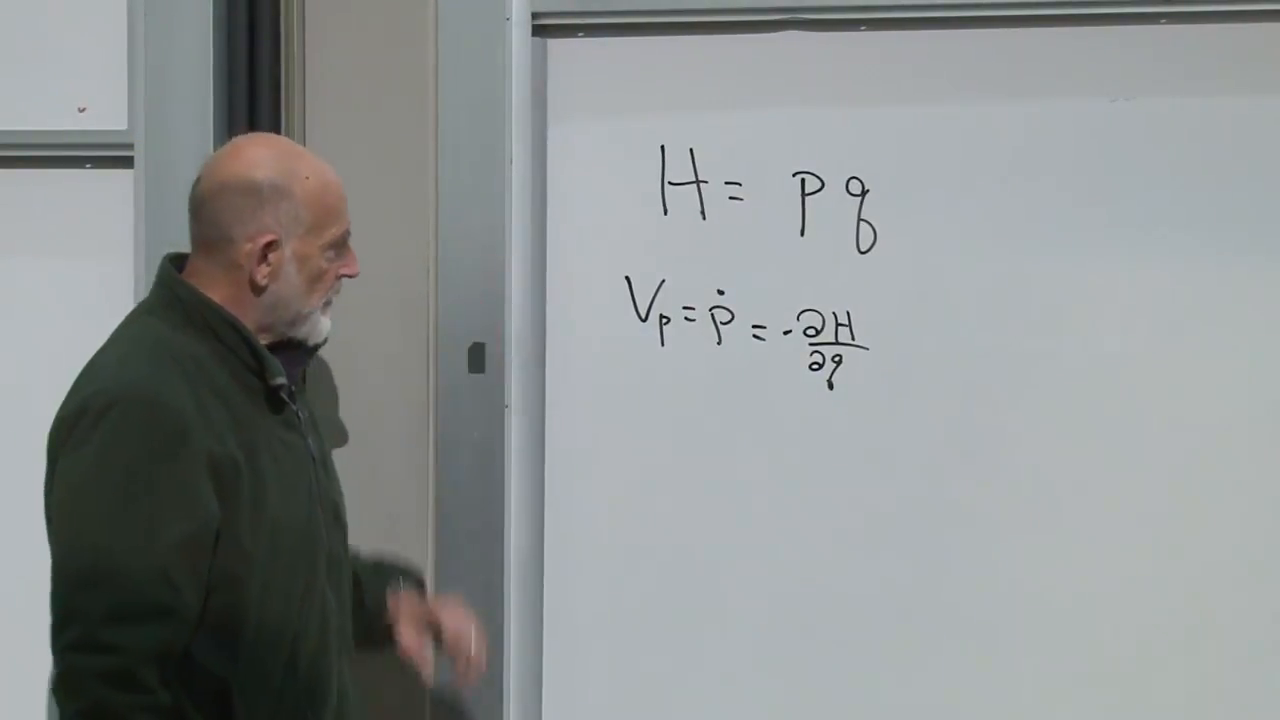
\includegraphics[width=0.82\textwidth]{lecture_07_figure_03.png}
  \caption{예제 \(H=pq\)의 시작 부분과 첫 번째 위상 공간 속도 성분.}
  \lectureframe{01:00:11}
\end{figure}

해밀턴 방정식은
\begin{equation}
  \dot p=-\lambda p,
  \qquad
  \dot q=\lambda q,
  \label{eq:l7-pq-flow}
\end{equation}
이며, 해는
\begin{equation}
  p(t)=p_0e^{-\lambda t},
  \qquad
  q(t)=q_0e^{\lambda t}.
  \label{eq:l7-pq-solutions}
\end{equation}
이다. 정사각형 패치는 \(p\) 방향으로 지수적으로 압축되고, 같은 인자만큼 \(q\) 방향으로 늘어난다.
\begin{equation}
  \Delta p(t)\Delta q(t)
  =
  \Delta p(0)\Delta q(0).
  \label{eq:l7-pq-area}
\end{equation}
발산을 계산해도 국소적으로 같은 결과를 확인할 수 있다.
\begin{equation}
  \frac{\partial\dot p}{\partial p}
  +\frac{\partial\dot q}{\partial q}
  =-\lambda+\lambda=0.
  \label{eq:l7-pq-divergence}
\end{equation}

\begin{figure}[htbp]
  \centering
  \includegraphics[width=0.86\textwidth]{lecture_07_figure_11.png}
  \caption{\(H=pq\) 흐름 아래에서 넓이를 보존하면서 길고 가느다란 띠로 늘어난 작은 패치.}
  \lectureframe{01:02:10}
\end{figure}

\begin{classroomqa}
  \audiencequestion{\(pq\)는 작용의 차원을 가지는데, 리우빌 정리는 작용 보존을 뜻하나요?\lecturetimestamp{01:03:00--01:04:09}}
  \lecturerresponse{아니다. 정리가 보존하는 것은 위상 공간 부피다. 정준 좌표쌍 하나에서 \(dq\,dp\)는 작용의 차원을 가지며, 이 차원적 사실은 위상 공간 셀의 크기를 \(\hbar\)가 정하는 양자역학을 예고한다. 그러나 곱 \(pq\) 자체는 해밀턴의 작용 범함수가 아니며, 차원이 같다는 이유만으로 각운동량이 되는 것도 아니다.}
\end{classroomqa}

이 예는 각도도 보존되지 않을 수 있음을 보여 준다. 식~\eqref{eq:l7-pq-solutions}의 스케일링 아래 성분들이 서로 다르게 변하는 직각 십자 모양은 계량상 전단되지만, 넓이는 그대로 유지된다. 리우빌 정리는 넓이 또는 부피에 관한 정리이지, 보통의 유클리드 강체성에 관한 정리가 아니다.

\section{감쇠는 흡인점을 만든다}

정리가 배제하는 것을 보려면 감쇠 진동자의 축약된 방정식을 살펴보자.
\begin{equation}
  m\ddot x=-kx-c\dot x,
  \qquad c>0.
  \label{eq:l7-damped-newton}
\end{equation}
\(p=m\dot x\)라 두면,
\begin{equation}
  \dot x=\frac{p}{m},
  \qquad
  \dot p=-kx-\frac{c}{m}p.
  \label{eq:l7-damped-first-order}
\end{equation}
감쇠가 없으면 위상점은 원점을 중심으로 돈다. 감쇠가 있으면 에너지가 주위 매질의 미시적 자유도로 전달되고 궤도는 안쪽으로 감긴다.

\begin{figure}[htbp]
  \centering
  \includegraphics[width=0.84\textwidth]{lecture_07_figure_13.png}
  \caption{감쇠 진동자의 방정식과 \(x\)-\(p\) 평면에서 안쪽으로 감기는 나선 궤도.}
  \lectureframe{01:13:30}
\end{figure}

이 2차원 축약 흐름의 발산은
\begin{equation}
  \frac{\partial\dot x}{\partial x}
  +\frac{\partial\dot p}{\partial p}
  =
  0-\frac{c}{m}<0.
  \label{eq:l7-damped-divergence}
\end{equation}
이다. 모든 유한한 패치는 수축한다. 원점은 흡인점이며, 연속적인 경우에 여러 화살표가 들어오는 상태에 해당한다.

\begin{figure}[htbp]
  \centering
  \includegraphics[width=0.88\textwidth]{lecture_07_figure_14.png}
  \caption{음의 발산 \(-c/m\)을 얻는 데 사용한 감쇠 위상 공간의 속도 성분.}
  \lectureframe{01:16:05}
\end{figure}

이는 미시적 역학이 리우빌 정리를 위반한다는 뜻이 아니다. 두 변수 \(x,p\)는 진동자의 에너지를 받아들이는 환경의 엄청난 수의 자유도를 생략한다. 진동자와 환경을 합친 확장 계는 해밀턴 계로서 부피를 보존할 수 있지만, 그 축약된 \(x,p\) 기술에서는 부피가 수축한다.

\begin{classroomqa}
  \audiencequestion{감쇠 진동자는 축약된 위상 공간에서 해밀턴 계가 아닌데도 여전히 뉴턴 방정식으로 기술되는가?
  \lecturetimestamp{01:20:09--01:21:12}}
  \lecturerresponse{그렇다. 뉴턴의 \(F=ma\)에는 경험적으로 주어지는 항력도 포함될 수 있다. 기본적인 \(L=T-V\) 및 해밀턴 기술은 보존력에 직접 적용되며, 더 일반적인 라그랑지안은 속도에 의존하는 힘의 일부도 다룬다. 그러나 고립된 한 쌍 \(x,p\)에 대한 마르코프 마찰항은 축약된 소산 동역학이지, 닫힌 정준 해밀턴 계가 아니다.}
\end{classroomqa}

\begin{classroomqa}
  \audiencequestion{감쇠 방정식을 무한한 정밀도로 역방향 적분할 수 있다면, 정보는 정말로 사라지는가?
  \lecturetimestamp{01:25:16--01:27:17}}
  \lecturerresponse{유한한 시간 동안에는 이상적인 미분 방정식에 여전히 역변환이 있으므로 정확한 자료를 역방향으로 계산할 수 있다. 정확한 진술은 유한한 위상 공간 셀의 부피가 지수적으로 수축한다는 것이다. 따라서 과거 상태를 복원하려면 정밀도를 지수적으로 높여야 하며, 무한한 시간이 지나면 모든 궤적은 흡인점에 접근한다. 이는 이산적인 대안 소실 그림에 가장 가까운 연속 고전적 유비이지, 유한한 시간 안에 두 정확한 해가 문자 그대로 하나가 된다는 주장은 아니다.}
\end{classroomqa}

\begin{classroomqa}
  \audiencequestion{발산이 0인 벡터장이 해밀턴 형식에서 나오지 않을 수도 있는가? \lecturetimestamp{01:18:21--01:22:34}}
  \lecturerresponse{물론이다. 해밀턴 형식은 발산이 0이 되기에 충분하지만 필수 조건은 아니다. 임의의 비압축성 속도장은 같은 공간에서 정준 해밀턴 벡터장이 아니더라도 발산이 0일 수 있다. 3차원 비압축성 유체의 속도장이 교과서적인 예다. 세 좌표만으로는 정준 쌍을 이룰 수 없다. 유체 역학 전체에는 더 정교한 무한 차원 해밀턴 형식이 존재할 수 있지만, 그렇다고 여기서 말한 한 방향의 함의가 뒤집히는 것은 아니다.}
\end{classroomqa}

\section{질문을 통해 드러나는 추가적인 구분}

\begin{classroomqa}
  \audiencequestion{일정한 에너지 곡면 위의 운동은 위상 공간 전체 부피의 보존과 어떤 관계가 있는가?
  \lecturetimestamp{01:28:47--01:30:41}}
  \lecturerresponse{두 현상은 해밀턴 구조에서 독립적으로 따르는 결과다. \(H\)가 시간에 명시적으로 의존하지 않으면, 각 궤적은 자기 에너지 곡면 위에 머문다. 유한한 영역은 여러 에너지 곡면을 가로지를 수 있지만, 리우빌 정리는 그 영역 전체의 부피가 보존된다고 말한다. 조화 진동자의 경우에는 흐름이 강체 회전이므로 영역의 모양도 유지된다. \(H=pq\) 영역은 넓이만 유지하고 모양은 유지하지 않는다.}
\end{classroomqa}

\begin{classroomqa}
  \audiencequestion{해밀턴 기술에서 역학적 일은 어떻게 다루는가? \lecturetimestamp{01:30:44--01:32:57}}
  \lecturerresponse{일은 선택한 계의 경계를 넘어 전달되는 에너지를 기술한다. 외부 작용자가 추를 들어 올리거나 매개변수를 바꾸어 부분계의 에너지를 변화시킬 수 있으며, 이때 공급한 에너지만큼 작용자의 에너지는 감소한다. 양쪽을 하나의 닫힌 모형에 포함하면, 초점은 전체 에너지의 보존과 부분계 사이의 에너지 교환으로 돌아간다.}
\end{classroomqa}

\begin{classroomqa}
  \audiencequestion{부피 보존은 위상과 각도도 보존하는가?
  \lecturetimestamp{01:33:00--01:33:37}}
  \lecturerresponse{매끄러운 유한 시간 해밀턴 흐름은 가역적인 연속 변형이므로 위상을 보존한다. 그러나 일반적으로 유클리드 각도나 모양은 보존하지 않는다. 진동자의 강체 회전에서는 보존되지만, \(H=pq\)의 신장은 그것이 특수한 경우임을 보여 준다.}
\end{classroomqa}

\begin{classroomqa}
  \audiencequestion{르장드르 변환은 물리적 의미가 없어서 생략되었는가?
  \lecturetimestamp{01:33:43--01:34:48}}
  \lecturerresponse{아니다. 속도 기술을 운동량 기술로 바꾸고, 사상이 정칙일 때 \(H=\sum_i p_i\dot q_i-L\)를 얻는 유용한 변환이다. 형식적인 이름을 강조하지 않았을 뿐, 이 구성은 이미 여러 차례 사용되었다. 다만 현재의 정리를 위해서는 일반 이론을 자세히 다룰 필요가 없다.}
\end{classroomqa}

\section{푸아송 괄호: 다음 단계의 압축}

마지막 몇 분 동안에는 다시 역사적 주제로 돌아간다. 19세기 역학은 겉보기에 서로 다른 계를 연결하는 간결한 구조를 거듭 모색했다---역학과 기하 광학, 입자와 광선, 고전 궤적과 파동적 기술이 그 예다. 푸아송 괄호도 그러한 구조의 하나이며, 양자역학에서 특히 중요해진다.

\(F(q,p)\)를 위상 공간 위의 임의의 함수라고 하자. 좌표나 운동량, 곱 \(qp\) 또는 각운동량일 수 있다. 운동을 따라 \begin{equation}
  \frac{dF}{dt}
  =
  \sum_i\left(
    \frac{\partial F}{\partial q_i}\dot q_i
    +\frac{\partial F}{\partial p_i}\dot p_i
  \right).
  \label{eq:l7-f-time-derivative}
\end{equation}
해밀턴 방정식을 대입하면 다음을 얻는다.
\begin{equation}
  \frac{dF}{dt}
  =
  \sum_i\left(
    \frac{\partial F}{\partial q_i}
    \frac{\partial H}{\partial p_i}
    -
    \frac{\partial F}{\partial p_i}
    \frac{\partial H}{\partial q_i}
  \right).
  \label{eq:l7-f-hamiltonian-derivative}
\end{equation}

\begin{figure}[htbp]
  \centering
  \includegraphics[width=0.88\textwidth]{lecture_07_figure_15.png}
  \caption{일반적인 위상 공간 함수 \(F(q,p)\)의 시간 미분에 대한 연쇄 법칙.}\lectureframe{01:42:40}
\end{figure}

반복해서 나타나는 반대칭 조합에 이름을 붙이자. 두 함수 \(F\)와 \(G\)의 푸아송 괄호를 다음과 같이 정의한다.
\begin{equation}
  \boxed{
  \{F,G\}
  =
  \sum_i\left(
    \frac{\partial F}{\partial q_i}
    \frac{\partial G}{\partial p_i}
    -
    \frac{\partial F}{\partial p_i}
    \frac{\partial G}{\partial q_i}
  \right).}
  \label{eq:l7-poisson-bracket}
\end{equation}

\begin{figure}[htbp]
  \centering
  \includegraphics[width=0.86\textwidth]{lecture_07_figure_16.png}
  \caption{두 함수의 미분 조합을 푸아송 괄호로 정의한 식.}\lectureframe{01:44:15}
\end{figure}

식~\eqref{eq:l7-f-hamiltonian-derivative}은 다음과 같이 된다.
\begin{equation}
  \boxed{\frac{dF}{dt}=\{F,H\}.}
  \label{eq:l7-hamiltonian-poisson-evolution}
\end{equation}
\(F\)도 시간에 명시적으로 의존하면 \(\partial F/\partial t\)를 더한다. \(F=q_i\) 또는 \(F=p_i\)를 대입하면 해밀턴의 두 방정식을 얻으므로, 식~\eqref{eq:l7-hamiltonian-poisson-evolution}은 전체 동역학을 간결하게 표현한다.

표기는 언제든 인위적으로 압축할 수 있다---여러 방정식을 제곱해 더한 뒤 하나의 방정식이라고 부를 수도 있다. 그렇게 하면 구조를 드러내기보다 감추게 된다. 푸아송 괄호가 유용한 이유는 정반대다. 푸아송 괄호의 대수 구조는 시간에 따른 변화, 보존량, 대칭을 체계화한다. 다음 단계에서는 그 대수 구조를 전개한 뒤, 고전역학과 양자 이론 모두에서 중심이 될 각운동량에 적용한다.

\section{가역성의 연속적인 의미}

이제 논리의 흐름을 줄이지 않고 진술할 수 있다. 해밀턴 방정식은 해밀토니안에 명시적인 시간 의존성이 없을 때 \(H\)를 보존하므로, 개별 궤적은 일정한 에너지 초곡면 위에 머문다. 같은 방정식은 위상 공간의 모든 점에 속도 벡터를 대응시킨다. 혼합 편미분들이 쌍으로 상쇄되므로 이 속도장의 발산은 사라진다. 따라서 가능한 상태들의 전체 영역은 정준 부피를 보존한다.

이것이 들어오는 화살표 하나와 나가는 화살표 하나에 해당하는 연속적인 경우다. 모양은 바뀔 수 있고, 각도도 바뀔 수 있으며, 이웃한 궤적들이 크게 벌어질 수도 있다. 매끄럽고 닫힌 해밀턴 기술에서는 유한한 대안들의 집합을 더 작은 위상 공간 부피로 압축할 수 없다. \(H=pq\) 흐름은 신장이 허용됨을 보여 준다. 축약된 감쇠 진동자는 해밀턴 조건을 버렸을 때 나타나는 흡인점을 보여 준다. 이어 푸아송 괄호는 해밀토니안이 모든 시간 미분을 생성한다는 진술로 같은 동역학을 압축한다.
\chapter{푸아송 괄호, 생성자, 각운동량}

\lectureoverview{푸아송 괄호는 해밀턴 방정식을 간결하게 다시 쓰는 방법에 그치지 않는다. 변환을 생성하는 대수적 연산이다. 해밀토니안과의 푸아송 괄호는 시간 변화를 생성하고, 운동량과의 푸아송 괄호는 병진을 생성하며, 각운동량과의 푸아송 괄호는 회전을 생성한다. 이 관점에서 대칭성과 보존은 하나의 푸아송 괄호가 영이 되는 현상을 서로 다르게 해석한 것이다. 조화 진동자에서 이 생각을 전개한 뒤, 오일러각을 도입하지 않고 각운동량 대수를 이용해 자이로스코프의 세차 운동을 구하겠다.}

\section{해밀턴 궤적을 따라 변하는 함수}

위상 공간에서 충분히 미분 가능한 함수 \[
  F=F(q_1,\ldots,q_n,p_1,\ldots,p_n)
\]를 생각하자. 이 함수는 두 가지 방식으로 볼 수 있다. 첫째, 위상 공간의 모든 점에 수를 하나 대응시킨다. 둘째, 해밀턴 궤적을 하나 정하면 점 \((q(t),p(t))\)가 움직이므로 시간의 함수가 된다. 그 궤적을 따라가면 \begin{equation}
  \frac{dF}{dt}
  =
  \sum_i\left(
    \frac{\partial F}{\partial q_i}\dot q_i
    +\frac{\partial F}{\partial p_i}\dot p_i
  \right).
  \label{eq:l8-chain-rule}
\end{equation} 해밀턴 방정식 \begin{equation}
  \dot q_i=\frac{\partial H}{\partial p_i},
  \qquad
  \dot p_i=-\frac{\partial H}{\partial q_i},
  \label{eq:l8-hamilton-equations}
\end{equation}을 대입하여 다음을 얻는다. \begin{equation}
  \frac{dF}{dt}
  =
  \sum_i\left(
    \frac{\partial F}{\partial q_i}
    \frac{\partial H}{\partial p_i}
    -
    \frac{\partial F}{\partial p_i}
    \frac{\partial H}{\partial q_i}
  \right).
  \label{eq:l8-fdot-expanded}
\end{equation} 오른쪽에 있는 이 조합은 두 항 가운데 어느 것도 해밀토니안이 아닌 경우에도 고전역학 전반에 걸쳐 나타난다. 이에 따라 다음과 같이 정의한다. \begin{equation}
  \boxed{
  \{F,G\}
  =
  \sum_i\left(
    \frac{\partial F}{\partial q_i}
    \frac{\partial G}{\partial p_i}
    -
    \frac{\partial F}{\partial p_i}
    \frac{\partial G}{\partial q_i}
  \right).}
  \label{eq:l8-poisson-definition}
\end{equation} 따라서 식 ~\eqref{eq:l8-fdot-expanded}은 다음과 같다. \begin{equation}
  \boxed{\dot F=\{F,H\}.}
  \label{eq:l8-time-generator}
\end{equation}

\begin{classroomqa} \audiencequestion{두 번째 항을 \(H\)에서 임의의 함수 \(G\)로 바꾸어도 괄호가 여전히 \(F\)의 시간 미분인가요? \lecturetimestamp{00:05:45--00:06:15}} \lecturerresponse{아니다. 표기법을 일반화하는 중에 청중이 중요한 점을 짚었다. 식 ~\eqref{eq:l8-poisson-definition}은 위상 공간의 임의의 두 함수에 대해 \(\{F,G\}\)를 정의하지만, \(\dot F=\{F,G\}\)은 \(G\)가 해밀토니안일 때만 성립한다. 일반적인 \(G\)는 다른 무한소 변환을 생성한다.}\end{classroomqa}

시간의 작은 변화를 다음과 같이 쓰면 편리하다. \begin{equation}
  \delta_t F=\epsilon\,\{F,H\}.
  \label{eq:l8-small-time-step}
\end{equation} 이 형태는 뒤에서 다룰 내용을 미리 보여 준다. 시간 변화는 푸아송 괄호로 생성되는 더 큰 변환 계열의 한 구성원이다.

\section{괄호 대수}

이제 괄호를 그 자체의 미적분으로 다룰 수 있다. 그 규칙은 보통의 미분에서 나온다. \begin{align}
  \{A,B\}&=-\{B,A\}, \label{eq:l8-antisymmetry}\\
  \{A+B,C\}&=\{A,C\}+\{B,C\}, \label{eq:l8-additivity}\\
  \{\lambda A,B\}&=\lambda\{A,B\},
    \quad \lambda\ \text{constant}, \label{eq:l8-scalar-rule}\\
  \{AB,C\}&=A\{B,C\}+\{A,C\}B. \label{eq:l8-leibniz}
\end{align} 이 네 줄은 각각 반대칭성, 가법성, 상수배에 대한 선형성, 라이프니츠 법칙을 나타낸다. 고전적 위상 공간 함수의 곱셈은 가환적이므로 마지막 줄에서 보통의 인수 \(A\)와 \(B\)의 위치는 중요하지 않다. 양자역학의 연산자에서는 더 이상 그렇지 않다. 반대칭성은 또한 다음을 함의한다. \begin{equation}
  \{A,A\}=0.
  \label{eq:l8-self-bracket}
\end{equation}

정준 좌표의 기본 푸아송 괄호는 다음과 같다.
\begin{equation}
  \boxed{
  \{q_i,q_j\}=0,\qquad
  \{p_i,p_j\}=0,\qquad
  \{q_i,p_j\}=\delta_{ij}.}
  \label{eq:l8-canonical-brackets}
\end{equation}
\(q_i\)에만 의존하는 함수는 \(q_i\)에만 의존하는 다른 함수와 푸아송 괄호가 영이다. \(p_i\)에만 의존하는 함수들에도 같은 성질이 성립한다. 푸아송 괄호가 영이 아니려면 정준 좌표와 그 켤레 운동량이 짝을 이루어야 한다. 식~\eqref{eq:l8-canonical-brackets}의 크로네커 델타는 지표가 서로 일치하는 경우에만 짝을 이룬다는 것을 나타낸다.

\subsection{조화진동자로 살펴보기}

다음을 생각하자. \begin{equation}
  H=\frac{p^2}{2m}+\frac{kq^2}{2}.
  \label{eq:l8-oscillator-hamiltonian}
\end{equation} 이제 괄호의 규칙과 식 ~\eqref{eq:l8-time-generator}만을 의도적으로 사용하겠다. 먼저, \begin{align}
  \dot q
  &=\{q,H\}\\
  &=\frac{1}{2m}\{q,p^2\}\\
  &=\frac{1}{2m}\left(p\{q,p\}+\{q,p\}p\right)\\
  &=\frac{p}{m}.
  \label{eq:l8-qdot-oscillator}
\end{align} 퍼텐셜 항은 \(\{q,q^2\}=0\)이므로 사라진다. 마찬가지로, \begin{align}
  \dot p
  &=\{p,H\}\\
  &=\frac{k}{2}\{p,q^2\}\\
  &=\frac{k}{2}\left(q\{p,q\}+\{p,q\}q\right)\\
  &=-kq.
  \label{eq:l8-pdot-oscillator}
\end{align} 여기서 음의 부호는 반대칭성 \(\{p,q\}=-\{q,p\}=-1\)에서 바로 나온다. 이 두 일차 방정식을 결합하면 다음을 얻는다. \begin{equation}
  m\ddot q=-kq.
  \label{eq:l8-hooke-equation}
\end{equation}

\begin{figure}[htbp]\centering
  
\includegraphics[width=0.82\textwidth]{lecture_08_figure_01.png}\caption{조화진동자 해밀토니안과 \(\dot q=p/m\) 및 \(\dot p=-kq\)을 얻는 두 푸아송 괄호 계산.}\lectureframe{00:23:20}\end{figure}

계산 도중, 강의실에서는 \emph{푸아송 괄호를 취하다}에 해당하는 동사를 찾다가 잠정적으로 \emph{푸아송화하다}를 쓰기로 한다. 이 농담은 관점의 실질적인 변화를 나타낸다. 대수를 알고 나면 정의에서 매번 결과를 다시 유도하지 않고 대수 자체를 바로 사용할 수 있다.

\begin{classroomqa}\audiencequestion{이 수학적 구조는 군인가요, 대수인가요? 역원이 있나요? \lecturetimestamp{00:23:48--00:24:16}} \lecturerresponse{군은 아니다. 괄호 연산은 군에 필요한 항등원과 역원을 제공하지 않는다. 위상 공간 함수들은 푸아송 대수를 이룬다. 보통의 가환적 곱셈과 덧셈에 더해, 반대칭 괄호가 있고 라이프니츠 법칙을 만족한다. 통상적인 추상적 정의를 완성하려면 야코비 항등식도 필요하지만, 이 강의에서는 다루지 않는다.}\end{classroomqa}

\begin{classroomqa}\audiencequestion{푸아송 괄호와 양자 교환자의 관계는 무엇인가요? \lecturetimestamp{00:24:18--00:25:00}} \lecturerresponse{강의에서는 미리보기만 제시한다. 양자역학으로 넘어갈 때 고전적 괄호는 개략적으로 다음과 같이 바뀐다. \[
    \{A,B\}_{\mathrm{PB}}
    \longleftrightarrow
    \frac{1}{i\hbar}[\widehat A,\widehat B].
  \] 이 대응에는 연산자 순서와 양자화에 관한 단서가 필요하며, 여기서는 정리로 사용하지 않는다.}\end{classroomqa}

조화진동자의 경우 괄호는 해밀턴 방정식을 다시 얻는 데 그쳤다. 괄호의 생성자가 \(H\) 이외의 보존량일 때 그 진가가 드러난다.

\section{회전 대칭성에서 각운동량 얻기}

강의 앞부분에서 다룬 뇌터 구성의 무한소 형태를 떠올려 보자. 연속 대칭에 의해 좌표가 \begin{equation}
  \delta q_i=\epsilon F_i(q),
  \label{eq:l8-noether-variation}
\end{equation}만큼 변한다면, 여기서 고려하는 경우 그 보존량은 \begin{equation}
  G=\sum_i p_iF_i(q).
  \label{eq:l8-noether-charge}
\end{equation}이다. 전체 인자 \(\epsilon\)는 생략해도 된다. 보존량에 고정된 수를 곱해도 보존 법칙은 바뀌지 않는다.

입자 하나를 \(z\)축 둘레로 무한소 회전시키자. 강의에서 사용한 방향 규약에 따르면, \begin{equation}
  \delta x=-\epsilon y,\qquad
  \delta y=\epsilon x,\qquad
  \delta z=0.
  \label{eq:l8-z-rotation}
\end{equation} 식 ~\eqref{eq:l8-noether-charge}을 적용하면 다음과 같다. \begin{equation}
  L_z=-p_xy+p_yx=xp_y-yp_x.
  \label{eq:l8-lz}
\end{equation} \(x\), \(y\), \(z\)을 순환적으로 바꾸면, \begin{equation}
  \boxed{\begin{aligned}
    L_x&=yp_z-zp_y,\\
    L_y&=zp_x-xp_z,\\
    L_z&=xp_y-yp_x.
  \end{aligned}}
  \label{eq:l8-angular-components}
\end{equation} 이는 다음의 성분이다. \begin{equation}
  \boldsymbol L=\boldsymbol r\times\boldsymbol p.
  \label{eq:l8-cross-product}
\end{equation}

\begin{figure}[htbp]\centering
  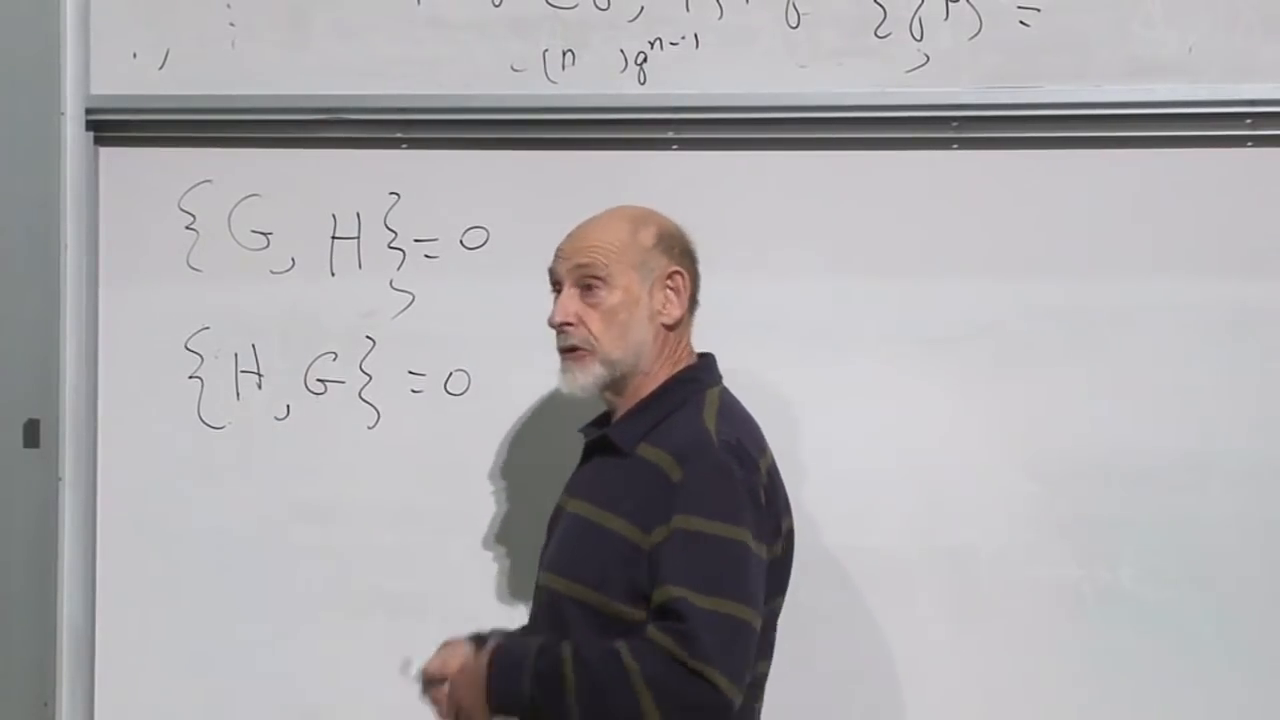
\includegraphics[width=0.82\textwidth]{lecture_08_figure_02.png}\caption{각운동량의 세 데카르트 성분과 이를 간결하게 나타낸 벡터곱 표현.}\lectureframe{00:34:00}\end{figure}

임의의 단위벡터 \(\boldsymbol n\)를 축으로 하는 회전은 \begin{equation}
  L_{\boldsymbol n}=\boldsymbol n\cdot\boldsymbol L.
  \label{eq:l8-arbitrary-axis}
\end{equation}에 의해 생성된다. 고립된 회전 대칭계에서는 세 성분이 모두 보존된다. 한 축 둘레의 회전만 대칭으로 남는다면, 그 축 방향 성분만 보존된다고 보장된다.

\section{각운동량은 회전을 생성한다}

회전 동역학 문제를 곧바로 풀기보다, 먼저 괄호를 취했을 때 \(L_z\)가 어떻게 작용하는지 살펴보자. 식 ~\eqref{eq:l8-lz}을 사용하면, \begin{align}
  \{x,L_z\}
  &=\{x,xp_y-yp_x\}
   =-y\{x,p_x\}
   =-y,\\
  \{y,L_z\}
  &=\{y,xp_y-yp_x\}
   =x\{y,p_y\}
   =x,\\
  \{z,L_z\}&=0.
  \label{eq:l8-position-rotation-brackets}
\end{align} 이는 식 ~\eqref{eq:l8-z-rotation}에 있는 계수와 정확히 일치한다.

\begin{figure}[htbp]\centering
  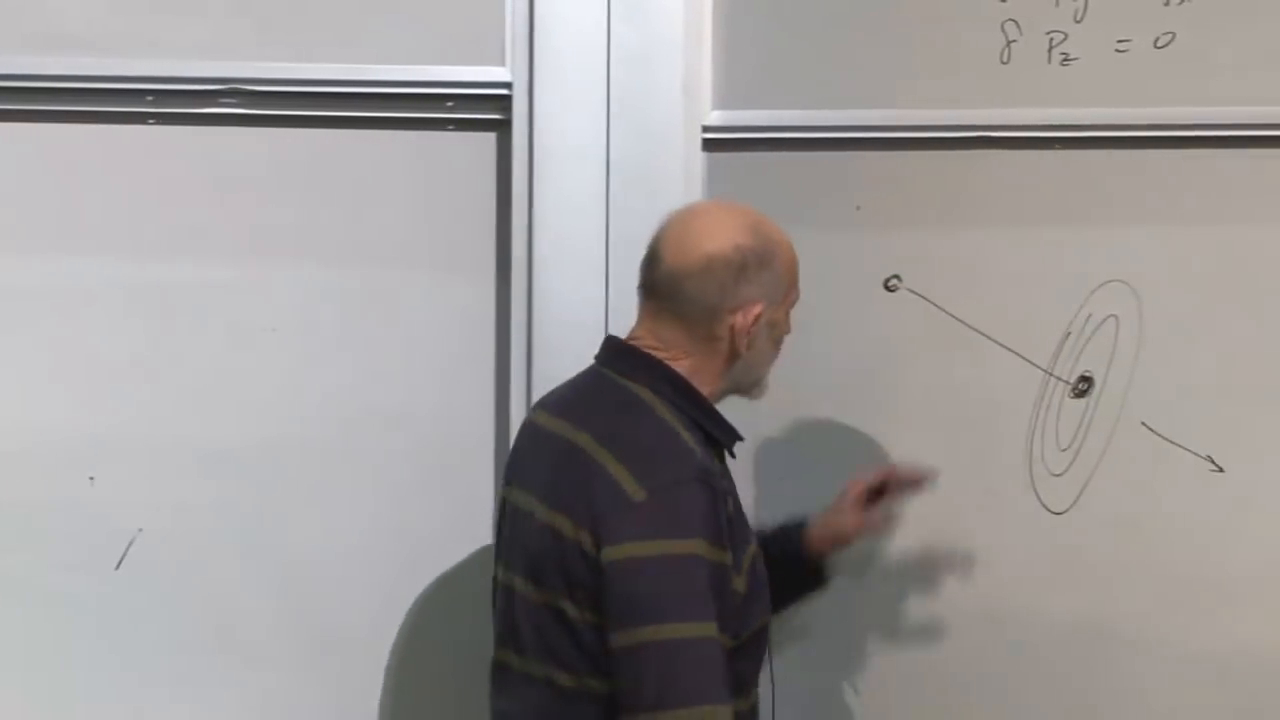
\includegraphics[width=0.82\textwidth]{lecture_08_figure_03.png}\caption{\(L_z\)와 좌표의 괄호: 괄호가 \((x,y,z)\)의 무한소 회전을 재현한다.}\lectureframe{00:38:41}\end{figure}

운동량도 벡터이므로 같은 계산을 하면 다음을 얻는다. \begin{equation}
  \begin{aligned}
    \{p_x,L_z\}&=-p_y,\\
    \{p_y,L_z\}&=p_x,\\
    \{p_z,L_z\}&=0.
  \end{aligned}
  \label{eq:l8-momentum-rotation-brackets}
\end{equation}

\begin{figure}[htbp]\centering
  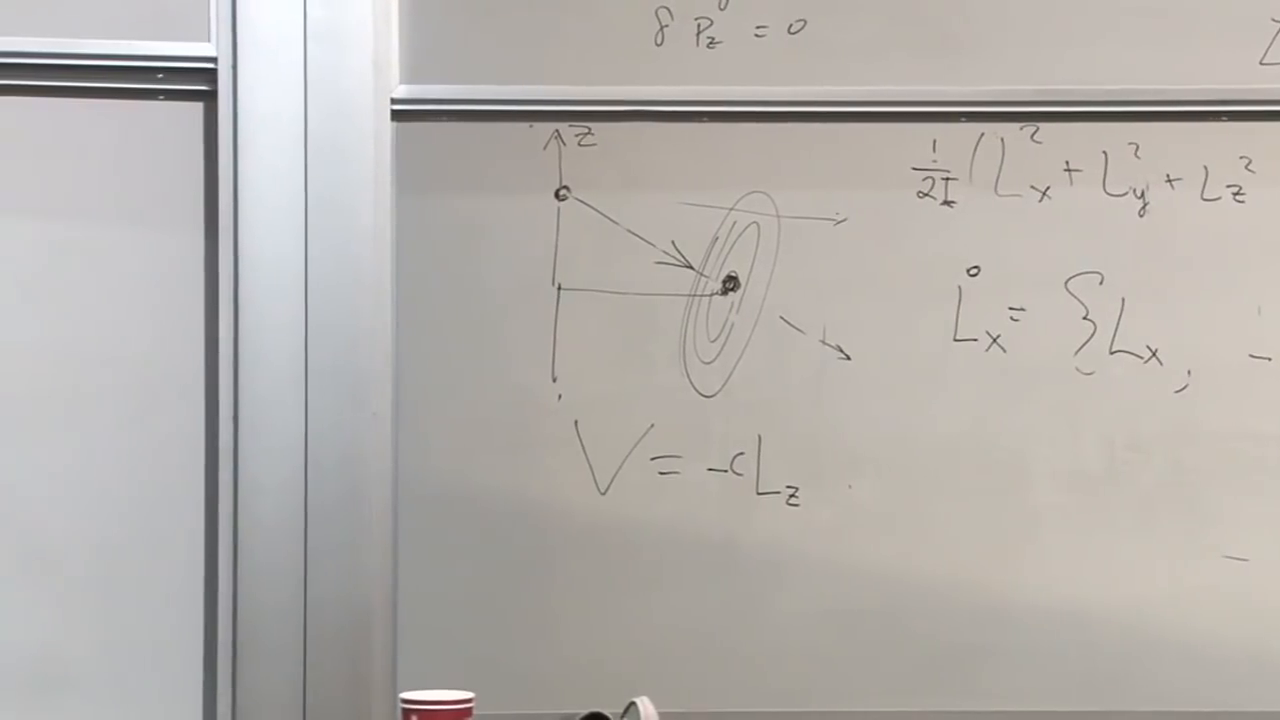
\includegraphics[width=0.82\textwidth]{lecture_08_figure_04.png}\caption{회전 생성자 \(L_z\)에 의해 위치와 운동량은 같은 벡터 형태로 변환된다.}\lectureframe{00:42:08}\end{figure}

따라서 일반적인 해밀턴 형식의 진술은 다음과 같다. \begin{equation}
  \boxed{\delta_G A=\epsilon\{A,G\}.}
  \label{eq:l8-generator-rule}
\end{equation} 위상 공간의 모든 함수 \(G\)는 이러한 무한소 정준 변환을 정의한다. \(G=L_z\)이면 회전이다. \(G=H\)이면 시간의 작은 변화이다.

\begin{classroomqa}\audiencequestion{강의에서는 어떤 때는 계를 회전시킨다고 하고, 어떤 때는 좌표를 회전시킨다고 합니다. 괄호 방정식에서는 어떤 규약을 쓰나요? \lecturetimestamp{00:28:22--00:29:35}} \lecturerresponse{식 ~\eqref{eq:l8-z-rotation}이 규약을 정한다. 이는 무한소 능동 회전 \((x,y)\mapsto(x-\epsilon y,y+\epsilon x)\)이다. 좌표축을 수동적으로 회전시키면 부호가 반대가 된다. 규약을 정하고 나면 괄호 공식은 모호하지 않다.}\end{classroomqa}

\section{운동량은 병진을 생성한다}

한 좌표 방향의 병진은 \begin{equation}
  \delta q=\epsilon.
  \label{eq:l8-q-translation}
\end{equation}이다. 여기서 식 ~\eqref{eq:l8-noether-variation}의 \(F(q)=1\)이므로, 이에 대응하는 보존량은 \(p\)이다. 생성자라는 주장은 다음을 예측한다. \begin{equation}
  \{f(q),p\}=\frac{df}{dq}.
  \label{eq:l8-translation-derivative}
\end{equation} 강의에서는 먼저 거듭제곱에 대해 귀납법으로 이를 증명한다. 기초 단계는 \(\{q,p\}=1\)이다. 다음을 가정하자. \begin{equation}
  \{q^{n-1},p\}=(n-1)q^{n-2}.
  \label{eq:l8-induction-hypothesis}
\end{equation} 그러면 곱의 법칙에 따라 \begin{align}
  \{q^n,p\}
  &=\{q\,q^{n-1},p\}\\
  &=q\{q^{n-1},p\}+\{q,p\}q^{n-1}\\
  &=(n-1)q^{n-1}+q^{n-1}\\
  &=nq^{n-1}.
  \label{eq:l8-power-translation}
\end{align} 선형성을 이용하면 이 결과를 다항식과 수렴하는 멱급수 표현으로 확장할 수 있다. 더 직접적으로는 괄호의 정의에서 미분 가능한 모든 \(f(q)\)에 대해 식 ~\eqref{eq:l8-translation-derivative}이 성립함을 알 수 있다. \begin{equation}
  \{f(q),p\}
  =
  \frac{\partial f}{\partial q}
  \frac{\partial p}{\partial p}
  =f'(q).
\end{equation}

\begin{figure}[htbp]\centering
  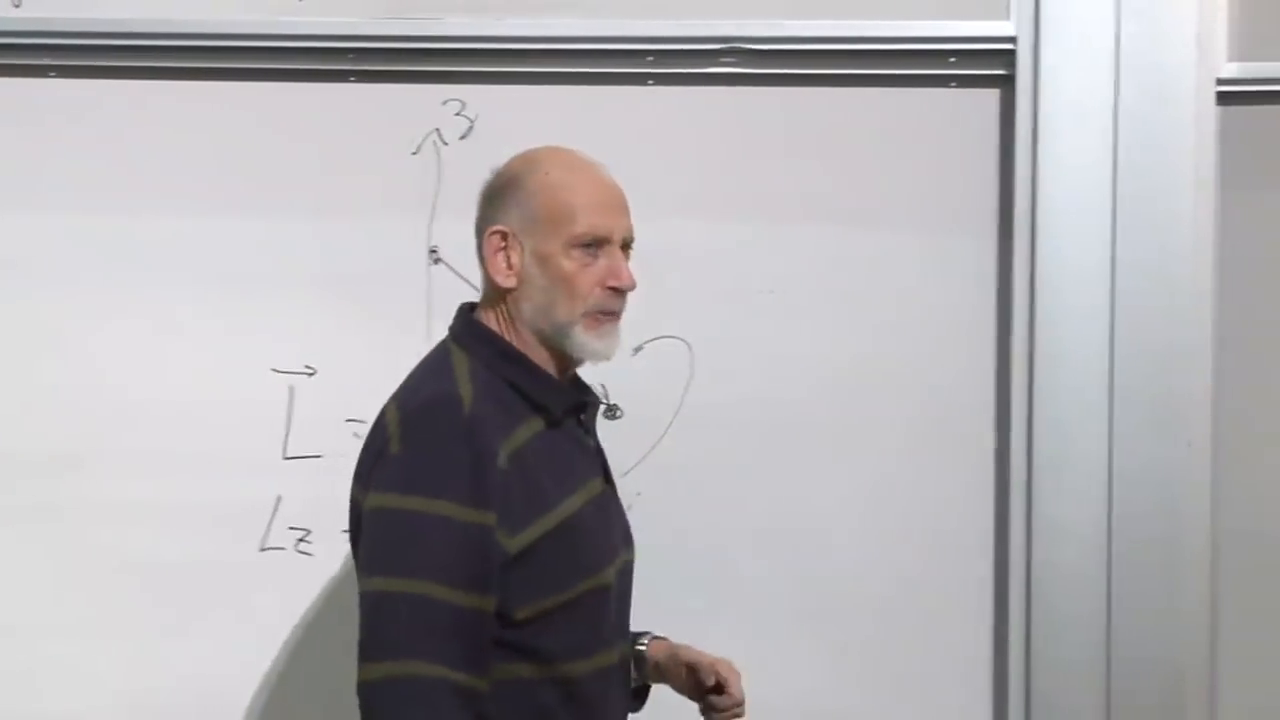
\includegraphics[width=0.82\textwidth]{lecture_08_figure_05.png}\caption{귀납법으로 얻은 병진 결과: \(\{F(q),p\}=dF/dq\).}\lectureframe{00:53:18}\end{figure}

이제 하나의 생각이 세 가지 형태로 나타남을 보았다. \begin{center}\begin{tabular}{@{}>{\raggedright\arraybackslash}p{0.37\textwidth}
                      >{\raggedright\arraybackslash}p{0.55\textwidth}@{}}\toprule
    생성자와 변환 &무한소 작용\\ \midrule
    \(H\)&\(\delta_tA=\epsilon\{A,H\}\)\\ \(p_i\)&\(\delta A=\epsilon\{A,p_i\}\)\\ \(L_i\)&\(\delta A=\epsilon\{A,L_i\}\)\\ \bottomrule
  \end{tabular}\end{center}연속 대칭에 대응하는 보존량은 그 대칭의 생성자이기도 하다.

\section{하나의 괄호, 두 가지 해석}

\(G(q,p)\)를 생성자 후보라고 하자. 이것이 보존되고 시간에 명시적으로 의존하지 않는다면, \begin{equation}
  \dot G=\{G,H\}=0.
  \label{eq:l8-g-conserved}
\end{equation} 반대칭성에 따라 \begin{equation}
  \{H,G\}=0.
  \label{eq:l8-h-invariant}
\end{equation} 수학적으로 두 식은 동등하지만, 물리적 해석은 다르다. \begin{itemize}\item \(\{G,H\}=0\)은 \(G\)가 \(H\)에 의해 생성되는 시간 변화 중에 변하지 않는다는 뜻이다. \item \(\{H,G\}=0\)은 \(H\)가 \(G\)에 의해 생성되는 변환 중에 변하지 않는다는 뜻이다.\end{itemize} 첫 번째는 보존 법칙이고 두 번째는 해밀토니안의 대칭성이다. 뇌터의 연결은 하나의 0으로 압축되어 있다.

\begin{figure}[htbp]\centering
  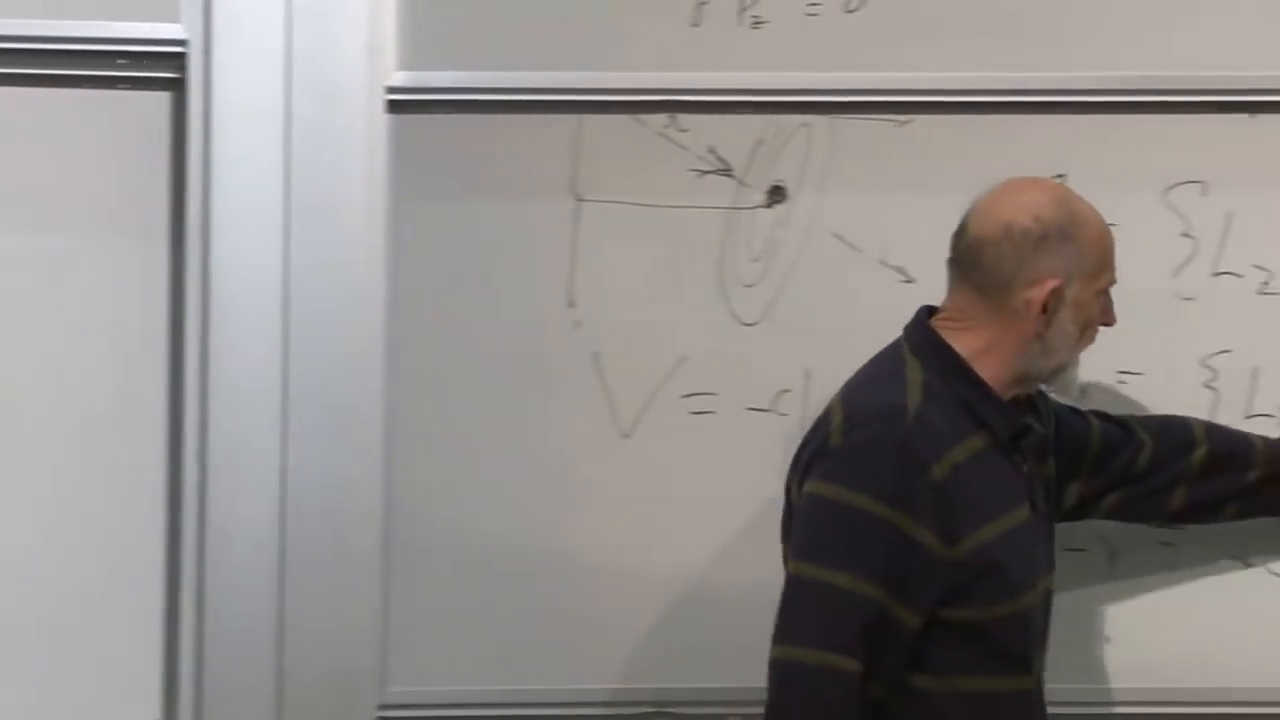
\includegraphics[width=0.82\textwidth]{lecture_08_figure_06.png}\caption{같은 영 괄호를 두 순서로 쓴 표현: \(G\)의 보존과 \(G\)가 생성하는 변환에 대한 \(H\)의 불변성.}\lectureframe{01:03:05}\end{figure}

\begin{classroomqa}\audiencequestion{보존량을 알고 있다면 그에 대응하는 대칭을 언제나 복원할 수 있나요? \lecturetimestamp{01:01:42--01:02:15}} \lecturerresponse{이 해밀턴 형식 안에서는 가능하다. 위상 공간 변수마다 \(G\)와 괄호를 취하면 된다. 그 결과인 모음 \(\delta_GA=\epsilon\{A,G\}\)은 변수들이 어떻게 변환되는지를 알려 준다. 예를 들어 \(L_z\)와의 괄호는 그 해석을 미리 몰랐더라도 회전을 드러낸다. 더 발전된 맥락에서는 전역적·경계 관련 미묘한 문제가 생길 수 있지만, 여기서는 국소적인 무한소 진술을 사용한다.}\end{classroomqa}

\begin{classroomqa}\audiencequestion{이 괄호 방정식은 보존 법칙을 일으키는 물리적 운동을 알려 주나요? \lecturetimestamp{00:56:01--00:58:13}} \lecturerresponse{아니다. 이 식들은 대칭 변환을 특정할 뿐 실제 궤적을 나타내지는 않는다. \(L_z\)의 보존은 회전 대칭을 뜻하지만, 입자가 원운동을 한다는 뜻은 아니다. 실제 시간 변화는 \(H\)에 의해 생성된다. 다른 생성자와의 괄호는 위상 공간에서 또 다른 변환 방향을 나타낸다.}\end{classroomqa}

\begin{classroomqa}\audiencequestion{보존을 미리 가정하지 않는 일반적인 변환 진술이 있나요? \lecturetimestamp{01:02:40--01:04:45}} \lecturerresponse{있다. 식 ~\eqref{eq:l8-generator-rule}은 함수 \(G\)마다 보존 여부와 관계없이 무한소 변환을 정의한다. 해밀토니안이 불변일 때만 대칭이 된다. 즉 \(\{H,G\}=0\)이다. 이를 반대 순서로 읽으면 \(G\)가 보존된다는 뜻이기도 하다.}\end{classroomqa}

\section{각운동량 대수}

다음 계산을 통해 회전 문제마다 입자 좌표를 계속 끌고 다니지 않아도 된다. 다음에서 시작하자. \[
  L_x=yp_z-zp_y,\qquad
  L_z=xp_y-yp_x.
\] \(\{L_x,L_z\}\)에서는 지수들이 정준쌍을 이루지 않으므로 대부분의 교차항이 사라진다. 남는 수축항을 계산하면 다음과 같다. \begin{align}
  \{L_x,L_z\}
  &=\{yp_z-zp_y,xp_y-yp_x\}\\
  &=xp_z-zp_x\\
  &=-L_y.
  \label{eq:l8-lx-lz}
\end{align} 순서를 바꾸면 음의 부호가 사라진다. 좌표를 순환적으로 바꾸면 다음을 얻는다. \begin{equation}
  \boxed{\begin{aligned}
    \{L_x,L_y\}&=L_z,\\
    \{L_y,L_z\}&=L_x,\\
    \{L_z,L_x\}&=L_y.
  \end{aligned}}
  \label{eq:l8-angular-algebra}
\end{equation} 지표 표기법으로는 다음과 같다. \begin{equation}
  \{L_i,L_j\}=\varepsilon_{ijk}L_k.
  \label{eq:l8-angular-algebra-index}
\end{equation}

\begin{figure}[htbp]\centering
  \includegraphics[width=0.82\textwidth]{lecture_08_figure_07.png}\caption{각운동량 세 성분의 순환 푸아송 괄호 대수.}\lectureframe{01:10:52}\end{figure}

이 결과는 미리 예측할 수도 있었다. \(\boldsymbol L\)는 벡터이므로, 그 \(x\) 성분과 \(L_z\)의 괄호는 \(z\)축 회전 아래 그 성분의 무한소 변화를 주어야 한다. 그 값은 \(-L_y\)이다. 명시적인 계산은 이 기하학적 논증을 확인해 준다. 이 방정식들은 양자 각운동량 교환 관계의 고전적 선구이기도 하다.

\section{빠르게 회전하는 자이로스코프}

응용으로 자이로스코프를 생각해 보자. 받침점에서 고정된 거리 \(R\)에 중심이 있는 고속 회전 플라이휠이다. 받침점에서 바퀴 중심을 향하는 벡터를 \(\boldsymbol r\)라 하자. 플라이휠은 축 둘레로 매우 빠르게 회전하므로, 지배적인 각운동량은 그 방향과 계속 나란하다. 강의에서 사용한 근사에서는 \begin{equation}
  \boldsymbol L=\ell\,\boldsymbol r,
  \qquad
  L_z=\ell z,
  \label{eq:l8-L-parallel-r}
\end{equation}이며, 여기서 \(\ell=L/R\)는 상수로 취급한다. 세차 운동이나 축의 운동에 관련된 더 작은 각운동량은 우선 무시한다.

\begin{figure}[htbp]\centering
  \begin{tikzpicture}[scale=0.95,>=Latex]
    \coordinate (P) at (0,3.2);
    \coordinate (C) at (3.7,1.55);
    \draw[->] (0,-0.2) -- (0,4.35) node[above] {\(z\)};
    \fill (P) circle (1.7pt) node[left] {pivot};
    \draw[very thick,->] (P) -- (C)
      node[midway,above right] {\(\boldsymbol r\parallel\boldsymbol L\)};
    \fill (C) circle (1.7pt);
    \draw[dashed] (P) -- (0,1.55);
    \draw[dashed] (0,1.55) -- (C);
    \node[left] at (0,1.55) {\(z\)};
    \begin{scope}[shift={(C)},rotate=-24]
      \draw[very thick] (0,0) ellipse (0.65 and 1.35);
      \draw[thick] (0,0) ellipse (0.42 and 0.9);
    \end{scope}
    \draw[->,thick] (2.15,2.85)
      arc[start angle=140,end angle=35,radius=1.65];
  \end{tikzpicture}\caption{빠른 자이로스코프 근사. 받침점과 중심 사이의 거리는 고정되어 있고, 지배적인 스핀 각운동량은 축 및 \(\boldsymbol r\)와 나란하게 유지된다.}\end{figure}

\begin{figure}[htbp]\centering
  \includegraphics[width=0.82\textwidth]{lecture_08_figure_08.png}\caption{플라이휠, \(H_{\rm rot}=L^2/(2I)\), 그리고 토크가 없을 때 \(\boldsymbol L\)가 보존됨을 보이는 소거를 칠판에 스케치한 그림.}\lectureframe{01:18:54}\end{figure}

\subsection{중력이 없을 때: 모든 성분이 고정되는 이유}

단순화한 축대칭 회전자의 경우, \begin{equation}
  H_{\mathrm{rot}}
  =\frac{1}{2I}
  \left(L_x^2+L_y^2+L_z^2\right)
  =\frac{L^2}{2I}.
  \label{eq:l8-rotational-hamiltonian}
\end{equation} 계수는 \(I/2\)이 아니라 \(1/(2I)\)이다. 칠판에서는 이 부분을 잘못 썼다가 바로잡는다. 식 ~\eqref{eq:l8-angular-algebra}을 사용하면, \begin{align}
  \dot L_x
  &=\{L_x,H_{\mathrm{rot}}\}\\
  &=\frac{1}{2I}\left(
    2L_y\{L_x,L_y\}
    +2L_z\{L_x,L_z\}
  \right)\\
  &=\frac{1}{I}\left(L_yL_z-L_zL_y\right)=0.
  \label{eq:l8-free-lx}
\end{align} 순환적으로 다음도 성립한다. \begin{equation}
  \dot L_x=\dot L_y=\dot L_z=0.
  \label{eq:l8-free-angular-momentum}
\end{equation} 스칼라 \(L^2\)는 각 성분 \(L_i\)과의 괄호가 0이다. 이 대수의 용어로는 카시미르이다. 따라서 토크가 없는 자이로스코프는 각운동량의 크기와 방향을 모두 유지한다.

\begin{classroomqa}\audiencequestion{여기서 관성 모멘트는 그냥 수 하나인가요? \lecturetimestamp{01:14:23--01:15:05}} \lecturerresponse{이 축약 모형에서는 그렇다. 관성 모멘트는 회전축에 대한 바퀴의 질량 분포를 나타낸다. 일반적인 강체에는 관성 모멘트 텐서가 있으며, 주축에서 회전 해밀토니안은 \(\sum_i L_i^2/(2I_i)\)이다. 이 강의에서는 완전한 강체 동역학을 전개하기보다 푸아송 괄호 방법을 보여 주려는 것이 목적이므로 더 단순한 고속 대칭 회전자를 택한다.}\end{classroomqa}

\subsection{중력과 퍼텐셜의 부호}

수직 좌표 \(z\)를 위쪽이 양의 방향이 되도록 잡고 받침점을 원점에 두자. 바퀴 중심의 중력 퍼텐셜 에너지는 \begin{equation}
  V=Mgz.
  \label{eq:l8-mgz}
\end{equation}이다. \(L_z=\ell z\)이므로, \begin{equation}
  V=cL_z,
  \qquad
  c=\frac{Mg}{\ell}=\frac{MgR}{L}.
  \label{eq:l8-potential-lz}
\end{equation}이다. 여기서 \(c>0\)은 \(\boldsymbol L\)가 \(\boldsymbol r\)와 평행하도록 정했을 때 성립한다. 플라이휠이 반대 방향으로 회전하면 \(\boldsymbol L\)와 \(\boldsymbol r\) 사이의 부호 있는 관계가 반전되며, 이에 따라 세차 각주파수의 부호도 바뀐다.

\begin{figure}[htbp]\centering
  \includegraphics[width=0.82\textwidth]{lecture_08_figure_09.png}\caption{\(\boldsymbol L=\ell\boldsymbol r\)와 \(L_z=\ell z\)에 해당하는 고정 길이 기하.}\lectureframe{01:25:38}\end{figure}

\begin{figure}[htbp]\centering
  \includegraphics[width=0.82\textwidth]{lecture_08_figure_10.png}\caption{칠판의 중간 단계에는 \(V=-cL_z\)가 나타난다. 나중에 \(z\)를 위쪽으로 정한 뒤 부호를 바로잡는다. \(\boldsymbol L=\ell\boldsymbol r\)와 \(\ell>0\)을 사용하면 일관된 결과는 \(V=+cL_z\)이다.}\lectureframe{01:22:43}\end{figure}

\begin{classroomqa}\audiencequestion{높이를 각운동량의 한 성분으로 바꾸어도 되는 이유는 무엇인가요? 비스듬한 선은 축인가요, 위치벡터인가요? \lecturetimestamp{01:22:20--01:25:43}} \lecturerresponse{비스듬한 선은 고정된 받침점에서 바퀴 중심까지의 벡터인 \(\boldsymbol r\)로 표시하는 것이 가장 적절하다. 실제 축이 그 방향을 따라 놓일 수는 있지만, 계산에서 사용하는 관계는 빠른 스핀 근사 \(\boldsymbol L=\ell\boldsymbol r\)이다. 따라서 두 벡터의 \(z\) 성분은 서로 비례한다. 실시간 강의에서는 이 구분을 확정하기 전에 표기를 몇 차례 바꾼다.}\end{classroomqa}

\begin{classroomqa}\audiencequestion{어떤 가정 아래서 \(\ell\)가 상수인가요? 바퀴 중심이 반지름 방향으로 미끄러질 수 있다면 무엇이 성립하지 않나요? \lecturetimestamp{01:25:43--01:26:38,\allowbreak\ 01:34:22--01:35:00}} \lecturerresponse{지배적인 스핀이 느린 운동에 따르는 각운동량보다 훨씬 크고, 받침점과 중심 사이의 거리가 고정되어 있다고 가정한다. 그러면 스핀의 크기는 거의 변하지 않고 \(\boldsymbol L\)는 \(\boldsymbol r\)와 함께 회전한다. 중심이 반지름 방향으로 미끄러질 수 있다면 \(z\)는 더 이상 하나의 상수 계수를 두고 \(L_z\)에 비례하지 않으므로, 축약 해밀토니안 \(V=cL_z\)으로는 운동을 기술할 수 없다.}\end{classroomqa}

\begin{classroomqa}\audiencequestion{칠판에 처음에는 음의 부호가 나오고 나중에는 양의 부호가 나오는 이유는 무엇인가요? 스핀 방향이 중요한가요? \lecturetimestamp{01:27:13--01:28:15,\allowbreak\ 01:33:09--01:33:21}} \lecturerresponse{처음의 부호는 칠판에 쓰는 도중의 오류와 정해지지 않은 축 규약이 섞인 결과다. \(z\)를 위쪽으로 정의하면 \(V=Mgz\)는 높이가 높아질수록 증가한다. \(\boldsymbol L=\ell\boldsymbol r\)와 \(\ell>0\)라면 \(V=+cL_z\)이다. 스핀을 반대로 하면 부호 있는 비례 관계와 세차 방향이 반전되지만, 임의로 부호를 선택해도 된다는 뜻은 아니다.}\end{classroomqa}

\subsection{세 개의 짧은 방정식으로 세차 운동 구하기}

축약된 전체 해밀토니안은 다음과 같다. \begin{equation}
  H=
  \frac{1}{2I}\left(L_x^2+L_y^2+L_z^2\right)+cL_z.
  \label{eq:l8-full-gyro-hamiltonian}
\end{equation} \(L^2\)는 모든 \(L_i\)와의 괄호가 0임을 이미 보였다. 따라서 선형 항만 기여한다. \begin{align}
  \dot L_z&=\{L_z,H\}=0,\\
  \dot L_x&=\{L_x,H\}=c\{L_x,L_z\}=-cL_y,\\
  \dot L_y&=\{L_y,H\}=c\{L_y,L_z\}=cL_x.
  \label{eq:l8-precession-equations}
\end{align}

\begin{figure}[htbp]\centering
  \includegraphics[width=0.82\textwidth]{lecture_08_figure_11.png}\caption{최종 성분 방정식: \(L_z\)는 일정하고 \(L_x\)와 \(L_y\)는 서로 변환되며 회전한다.}\lectureframe{01:30:35}\end{figure}

수직 성분과 수평 성분의 크기는 일정하다. \begin{equation}
  \frac{d}{dt}(L_x^2+L_y^2)
  =2L_x(-cL_y)+2L_y(cL_x)=0.
\end{equation} 수평 성분을 결합하면, \begin{equation}
  L_+=L_x+iL_y,
  \qquad
  \dot L_+=icL_+,
\end{equation} 따라서 \begin{equation}
  L_+(t)=L_+(0)e^{ict}.
  \label{eq:l8-precession-solution}
\end{equation} 각운동량 벡터는 수직축 둘레로 각속력 \(|c|=MgR/L\)로 세차한다. 이 이상화된 정상 운동에서는 기울기가 일정하게 유지된다.

\begin{classroomqa}\audiencequestion{세차 방정식을 쓸 때 회전 에너지 항을 무시했나요? \lecturetimestamp{01:35:01--01:35:49}} \lecturerresponse{아니다. 식 ~\eqref{eq:l8-full-gyro-hamiltonian}처럼 전체 해밀토니안에 포함된다. 다만 \(\dot L_i\)에 기여하지 않을 뿐이다. \(\{L_i,L^2\}=0\)이기 때문인데, 이는 토크가 없는 경우의 계산에서 이미 증명한 소거이다. 학생의 질문 덕분에 암묵적이었던 이 단계가 명시되었다.}\end{classroomqa}

\begin{classroomqa}\audiencequestion{균일 세차는 평형 상태인가요? 작은 충격을 주면 어떻게 되나요? \lecturetimestamp{01:32:38--01:33:08}} \lecturerresponse{정적인 평형 상태라기보다 정상 운동 또는 정상 상태의 운동이라고 부르는 편이 정확하다. 작은 충격을 주면 일반적으로 장동, 즉 기울기 각도의 진동이 더해진다. 매우 빠르게 회전하는 바퀴에서는 그 진동이 작으므로 축약된 설명에서는 거의 균일한 세차만 고려한다.}\end{classroomqa}

\begin{classroomqa}\audiencequestion{세차 운동에는 지지대나 실제 축이 필요한가요? \lecturetimestamp{01:31:49--01:32:38,\allowbreak\ 01:33:49--01:35:00}} \lecturerresponse{이 역학 모형에서는 받침점과 중심 사이의 거리가 고정되어 있다고 가정하므로, 어떤 구속력이 지지 역할을 한다. 더 일반적인 대수적 결과는 적용 범위가 넓다. 각운동량의 한 성분에 선형인 해밀토니안 항이 있으면 언제나 같은 괄호 대수로 세차 운동을 얻는다. 각운동량의 미시적 근원이 실제 축에 달린 바퀴일 필요는 없다.}\end{classroomqa}

\begin{classroomqa}\audiencequestion{이것은 자기장 속 전자 스핀이나 핵스핀의 세차 운동, 또는 행성 궤도의 세차 운동과 같은 현상인가요? \lecturetimestamp{01:35:50--01:37:00}} \lecturerresponse{자기장과 결합한 자기 모멘트는 스핀 성분에 선형인 해밀토니안을 가지므로 같은 각운동량 대수를 따른다. 핵스핀의 세차 운동은 핵자기공명에 쓰인다. 행성 궤도 근일점의 세차는 \emph{세차}라는 말을 공유할 뿐 다른 현상이며, 같은 계산이 아니다.}\end{classroomqa}

\begin{classroomqa}\audiencequestion{옆으로 장착된 자이로스코프는 본질적으로 팽이와 같은 물체인가요? \lecturetimestamp{01:37:02--01:37:23}} \lecturerresponse{그렇다. 차이는 주로 기하학적 표현에 있다. 회전축이 지지대에서 옆으로 뻗어 있을 때는 보통 자이로스코프라 하고, 거의 수직일 때는 팽이라고 한다. 각운동량과 토크의 구조는 같다.}\end{classroomqa}

\section{계산을 통해 얻은 것}

오일러각을 도입하지 않았고 바퀴의 모든 부분에 대한 좌표를 추적하지도 않았다. \[
  \{L_i,L_j\}=\varepsilon_{ijk}L_k
\]을 알고 나면 관심 있는 변수들의 방정식을 바로 얻을 수 있다. 이것이 보여 주려는 힘이다. 조화진동자에서는 푸아송 괄호가 익숙한 동역학을 재현할 수 있음을 보았다. 각운동량은 푸아송 괄호가 그 이상의 일을 한다는 점을 보여 주었다. \begin{itemize}\item 보존량은 그에 대응하는 무한소 대칭을 생성한다. \item \(G\)의 보존과 \(H\)의 불변성은 \(\{G,H\}=0\)의 두 가지 해석이다. \item 관측량의 대수는 그 자체 안에서 닫힐 수 있어 미시적 좌표로 되돌아가지 않고도 동역학을 풀 수 있다. \item 각운동량 성분 하나에 선형인 해밀토니안은 그 축 둘레의 세차 운동을 일으킨다.\end{itemize}강의는 일반적인 강체에 대한 완전한 오일러 방정식을 다루기 전에 끝난다. 그보다 좁은 결론은 이미 완결되었다. 적절한 생성자와 그 푸아송 대수는 대칭과 운동을 놀라울 만큼 간결하게 드러낸다.\chapter{자기력, 벡터 퍼텐셜, 작용 원리}

\lectureoverview{정전기력은 익숙한 보존력의 형태를 따르지만, 자기력은 속도에 의존합니다. 이를 라그랑주 역학에 포함하기 위해 먼저 필요한 벡터 미적분을 살펴보고, 자기장이 원천이 없다는 성질을 이용해 벡터 퍼텐셜을 도입한 뒤, 그 게이지 자유도를 검토하고 작용에 들어가는 자기 항을 구성합니다.}

\section{새로운 종류의 힘}

앞서 각운동량, 자이로스코프, 푸아송 괄호를 논의하면서 몇 가지 주제가 한데 모였습니다. 특히 자기장 속에서 회전하는 대전 물체는 자이로스코프와 매우 비슷하게 세차 운동을 합니다. 이제 그 유비에서 벗어나 개별 대전 입자의 운동을 살펴보겠습니다.

정전기력에는 새로운 역학이 필요하지 않습니다. \(U(\mathbf x)\)이 퍼텐셜 에너지라면,
\begin{equation}
  \mathbf F=-\nabla U(\mathbf x),
\end{equation}
익숙한 논증을 통해 운동 에너지와 퍼텐셜 에너지의 합이 보존됨을 알 수 있습니다. 정전기 퍼텐셜 \(V(\mathbf x)\) 속에서 전하 \(e\)를 띤 입자의 경우,
\begin{equation}
  U(\mathbf x)=eV(\mathbf x),
  \qquad
  \mathbf F_{\mathrm{el}}=-e\nabla V.
\end{equation}
자기력은 형태가 다릅니다. 입자의 속도에 의존하므로 보통의 퍼텐셜 에너지를 하나 더하는 것만으로는 도입할 수 없습니다. 그럼에도 자기력은 작용 원리에서 유도되며 라그랑지안과 해밀토니안으로 기술할 수 있습니다. 이를 위해서는 벡터 미적분을 짧지만 꼭 필요한 중간 과정으로 살펴봐야 합니다.

\section{장과 국소 연산}

\subsection{장이 나타내는 것}

장은 공간의 모든 점에, 일반적으로는 모든 시각에 물리량을 대응시킵니다. 온도와 압력은 스칼라장이고, 바람의 속도는 벡터장입니다. 전기장과 자기장도 벡터장입니다. 다른 이론에는 미시적 규모에서도 스칼라장이 등장하고, 중력은 텐서장으로 기술됩니다. 여기서는 시간에 따른 변화는 생략하고 장을 \(\mathbf x\)의 함수로 나타내겠습니다.

장에서 실질적으로 중요한 점은 국소성입니다. 어떤 영역이 가방 안에 가려져 있다고 상상해 봅시다. 그 영역의 전기장을 측정하려면 작은 시험 전하를 그곳에 놓고 가속도를 관측하면 됩니다. 힘은 전하가 놓인 곳의 장으로 정해지며, 멀리 떨어진 모든 원천에 따로 문의해야 하는 것이 아닙니다. 자기장과 움직이는 시험 전하에도 같은 설명이 적용됩니다. 뒤에서 벡터 퍼텐셜을 다룰 때 이 단순한 그림에 단서를 붙이겠지만, 여기서 출발하는 것이 적절합니다.

\subsection{미분 연산자}

미분하면 장에서 다른 장을 얻습니다. 세 공간 미분을 다음과 같이 모아 씁니다.
\begin{equation}
  \nabla
  =
  \left(
    \frac{\partial}{\partial x},
    \frac{\partial}{\partial y},
    \frac{\partial}{\partial z}
  \right).
\end{equation}
이 기호는 \emph{델} 또는 \emph{나블라}라고 읽습니다. 거꾸로 된 삼각형 모양은 기억하기 쉽지만, 진짜 의미는 성분이 미분 연산자인 벡터처럼 형식적으로 작용한다는 데 있습니다.

이는 보통의 3차원 물리 공간이지, 위상 공간도 아니고 다입자 배치 공간도 아닙니다. 더구나 \(\nabla\)는 그 자체로 놓일 수 있는 벡터장이 아닙니다. 반드시 어떤 대상에 작용해야 합니다. \(T(\mathbf x)\)가 스칼라 온도장이라면,
\begin{equation}
  \nabla T
  =
  \left(
    \frac{\partial T}{\partial x},
    \frac{\partial T}{\partial y},
    \frac{\partial T}{\partial z}
  \right)
\end{equation}
는 그 기울기, 즉 진짜 벡터장입니다.

\begin{figure}[htbp]
\centering
\includegraphics[width=0.82\textwidth]{lecture_09_figure_01.png}
\caption{\(\nabla\)를 공간 미분 연산자의 벡터로 소개하고 스칼라장 \(T(\mathbf x)\)에 적용하기 시작한다.}
\lectureframe{00:11:30}
\end{figure}

스칼라는 단지 성분 하나로 적는 양이 아닙니다. 좌표축의 방향과 무관하게 값이 정해지는 양입니다. 온도가 대표적인 예입니다. 벡터장 \(\mathbf E\)가 주어졌을 때 국소적인 표현 \(\mathbf E\cdot\mathbf E\)도 스칼라입니다. 반면 장을 적분하여 퍼텐셜을 구성하는 일은 비국소 연산입니다. 경로를 따라 여러 지점의 값을 사용합니다.

\subsection{발산}

벡터장 \(\mathbf A=(A_x,A_y,A_z)\)에 대해 스칼라
\begin{equation}
  \nabla\cdot\mathbf A
  =
  \frac{\partial A_x}{\partial x}
  +\frac{\partial A_y}{\partial y}
  +\frac{\partial A_z}{\partial z}
\end{equation}
를 발산이라고 합니다. 유체의 관점에서 양의 발산은 국소적으로 바깥쪽으로 흘러나가려는 경향을, 음의 발산은 안쪽으로 모여들려는 경향을 나타냅니다. 유체의 원천에서는 발산이 양수이고, 흡수원에서는 음수입니다. 이는 정성적인 그림이지만, 자기장에 원천이 없다는 성질을 분명하게 보여 줄 것입니다.

\section{외적, 엡실론 기호, 회전}

\subsection{성분으로 나타낸 외적}

두 벡터 \(\mathbf V\)와 \(\mathbf A\)의 외적 성분 하나는 다음과 같습니다.
\begin{equation}
  (\mathbf V\times\mathbf A)_x
  =
  V_yA_z-V_zA_y.
\end{equation}
나머지 두 성분은 \(x\to y\to z\to x\)의 순환에 따라 얻습니다. \(x,y,z\) 대신 \(1,2,3\) 지표를 쓰면 편리합니다. 크로네커 기호는
\begin{equation}
  \delta_{ij}
  =
  \begin{cases}
    1,&i=j,\\
    0,&i\ne j,
  \end{cases}
\end{equation}
이고 레비--치비타 기호는 다음과 같이 정의됩니다.
\begin{equation}
  \epsilon_{123}=\epsilon_{231}=\epsilon_{312}=1,
  \qquad
  \epsilon_{132}=\epsilon_{321}=\epsilon_{213}=-1,
\end{equation}
두 지표가 같으면 \(\epsilon_{ijk}=0\)입니다. 세 시간 시계 방향의 순환 순서는 양의 부호를, 그 반대 방향은 음의 부호를 줍니다. 두 지표를 맞바꾸면 부호가 바뀌므로 \(\epsilon_{ijk}\)는 완전 반대칭입니다.

또한 합산 규약을 사용합니다. 항 안에서 반복되는 지표는 \(1\)부터 \(3\)까지 합산합니다. 그러면 외적의 세 성분 방정식은 다음과 같이 됩니다.
\begin{equation}
  (\mathbf V\times\mathbf A)_i
  =
  \epsilon_{ijk}V_jA_k.
\end{equation}
예를 들어 \(i=1\)로 놓으면 \((j,k)=(2,3)\)와 \((3,2)\)만 남습니다.
\begin{equation}
  (\mathbf V\times\mathbf A)_1
  =
  \epsilon_{123}V_2A_3
  +\epsilon_{132}V_3A_2
  =
  V_2A_3-V_3A_2.
\end{equation}
따라서 간결한 표기에는 익숙한 성분 규칙이 그대로 담겨 있습니다.

\subsection{반대칭 행렬로 나타낸 벡터}

두 번째 표현은 다음과 같습니다.
\begin{equation}
  V_iA_j-V_jA_i
  =
  \epsilon_{ijk}(\mathbf V\times\mathbf A)_k.
\end{equation}
왼쪽은 두 개의 첨자를 가지며 \(i\leftrightarrow j\)에 대해 반대칭입니다. 행렬로 쓰면 다음과 같은 형태입니다.
\begin{equation}
  M_{ij}
  =
  \begin{pmatrix}
    0&M_{12}&M_{13}\\
    -M_{12}&0&M_{23}\\
    -M_{13}&-M_{23}&0
  \end{pmatrix}.
\end{equation}
대각 성분은 모두 사라지고, 아래쪽 삼각 부분은 위쪽 삼각 부분에 의해 정해집니다. 따라서 독립적인 성분은 세 개입니다.

\begin{figure}[htbp]
\centering
\includegraphics[width=0.82\textwidth]{lecture_09_figure_02.png}
\caption{외적의 한 성분과 독립적인 성분을 세기 위한 도식적인 \(3\times3\) 반대칭 배열. 칸 안의 표시는 기억을 돕기 위한 것이며 별도의 기호가 아니다.}
\lectureframe{00:34:20}
\end{figure}

\begin{classroomqa}
\audiencequestion{외적이나 이를 다른 벡터와 동일시하는 것이 3차원 밖에서도 성립하나요?}
\lecturerresponse{두 지표를 가진 반대칭 대상은 어떤 차원에서도 정의되지만, 이를 벡터와 동일시하는 것은 3차원에만 특별히 성립합니다. 3차원 벡터의 성분 수는 세 개이고, 반대칭 \(3\times3\) 행렬의 독립 성분 수도 세 개입니다. 4차원에서는 각각 네 개와 여섯 개인데, \(4(4-1)/2=6\)이기 때문입니다. 반대칭 대상은 여전히 존재하며 자연스럽게 2형식으로 볼 수 있지만, 또 하나의 4-벡터는 아닙니다.}
\end{classroomqa}

\subsection{회전}

\(\mathbf V\)를 \(\nabla\)로 바꾸면 회전을 정의합니다.
\begin{equation}
  (\nabla\times\mathbf A)_i
  =
  \epsilon_{ijk}\frac{\partial A_k}{\partial x_j}.
\end{equation}
일반적인 성분으로 쓰면 다음과 같습니다.
\begin{align}
  (\nabla\times\mathbf A)_x
  &=
  \frac{\partial A_z}{\partial y}
  -\frac{\partial A_y}{\partial z},\\
  (\nabla\times\mathbf A)_y
  &=
  \frac{\partial A_x}{\partial z}
  -\frac{\partial A_z}{\partial x},\\
  (\nabla\times\mathbf A)_z
  &=
  \frac{\partial A_y}{\partial x}
  -\frac{\partial A_x}{\partial y}.
\end{align}
발산이 국소적으로 퍼져 나가는 정도를 측정한다면, 회전은 국소적인 순환을 측정합니다. 축을 중심으로 회전하는 유체는 그 축 방향으로 회전을 가집니다. 이 그림은 특히 속도장에서 선명하게 드러나지만, 이 정의는 모든 벡터장에 적용됩니다.

\section{두 가지 구조적 항등식}

수학적 전개의 대부분은 다음 두 사실로 해결됩니다.
\begin{equation}
  \nabla\cdot(\nabla\times\mathbf A)=0,
  \qquad
  \nabla\times(\nabla s)=0.
\end{equation}
첫 번째는 이계 도함수는 대칭인 반면 \(\epsilon_{ijk}\)는 반대칭이라는 점에서 나옵니다.
\begin{equation}
  \nabla\cdot(\nabla\times\mathbf A)
  =
  \epsilon_{ijk}\partial_i\partial_j A_k
  =0.
\end{equation}
두 번째는 혼합 편미분의 순서를 바꿔도 같다는 데서 나옵니다.
\begin{equation}
  \bigl[\nabla\times(\nabla s)\bigr]_i
  =
  \epsilon_{ijk}\partial_j\partial_k s
  =0.
\end{equation}

\begin{figure}[htbp]
\centering
\includegraphics[width=0.80\textwidth]{lecture_09_figure_03.png}
\caption{칠판에 적힌 첫 번째 항등식: 모든 회전의 발산은 사라집니다.}
\lectureframe{00:38:26}
\end{figure}

이 두 방향은 간단하므로, 강의에서 예고한 숙제나 쪽지 시험에 적합합니다. 역방향 명제에는 좀 더 주의가 필요합니다. 국소적으로, 또는 적절하게 단일연결이거나 수축 가능한 영역 전체에서,
\begin{align}
  \nabla\cdot\mathbf F=0
  &\quad\Longrightarrow\quad
  \mathbf F=\nabla\times\mathbf A,\\
  \nabla\times\mathbf F=0
  &\quad\Longrightarrow\quad
  \mathbf F=\nabla s.
\end{align}
영역에 대한 단서를 붙이지 않으면 구멍이나 다른 전역 위상적 특성이 이러한 결론을 막을 수 있습니다. 여기서는 아래에서 필요한 바로 그 국소적 형태를 사용합니다.

\section{자기장은 왜 회전으로 나타내는가}

\subsection{관측된 자기 원천은 없다}

자기장 \(\mathbf B\)은 대전 입자와 전류에 미치는 영향으로 조작적으로 정의됩니다. 자기 홀극이 없는 보통의 전자기학에서는,
\begin{equation}
  \nabla\cdot\mathbf B=0.
\end{equation}
이는 발산이 전하 밀도에 비례하는 전기장과 다릅니다. 전하는 전기 선속의 원천이자 흡수원입니다. 자기 선속의 고립된 원천이나 흡수원은 관측된 적이 없습니다.

자기 홀극이 있다면 이 방정식은 달라질 것입니다. 통일장 이론은 이런 물체가 존재할 것이라는 이론적 근거를 제시하는 경우가 많지만, 실제로 존재하더라도 현재 가능한 실험에서 만들어 내기에는 질량이 너무 클 수 있습니다. 따라서 여기서는 자기 전하 밀도가 0인 이론을 다룹니다.

\begin{classroomqa}
\audiencequestion{자기 홀극이란 무엇인가요? 보통 자석에도 이미 북극과 남극이 있잖아요.}
\lecturerresponse{고립된 홀극은 전하와 비슷하게 자기장의 진짜 원천 또는 흡수원입니다. 보통의 막대자석은 다릅니다. 북극 근처에서 나오는 자기력선은 공간을 지나 남극으로 되돌아오고, 자석 물질 내부를 계속 이어서 통과합니다. 외부에서 원천과 흡수원처럼 보이는 것은 숨겨진 관을 통해 흐르는 유체처럼 서로 이어져 있습니다. 자기 선속이 순생성되거나 소멸하지 않습니다.}
\end{classroomqa}

\begin{figure}[htbp]
\centering
\includegraphics[width=0.76\textwidth]{lecture_09_figure_04.png}
\caption{그림은 북극과 남극이 원천처럼 보이는 모습을 대비하면서, 자석 안쪽에서 자기력선을 이어 자기 선속이 그곳에서 시작하거나 끝나지 않음을 강조한다.}
\lectureframe{00:44:56}
\end{figure}

\(\mathbf B\)의 발산이 없으므로, 역정리를 이용해 적어도 국소적으로는 다음과 같이 쓸 수 있습니다.
\begin{equation}
  \boxed{\mathbf B=\nabla\times\mathbf A}.
\end{equation}
장 \(\mathbf A\)를 벡터 퍼텐셜이라고 합니다. 처음에는 측정 가능한 장 \(\mathbf B\)을 불필요하게 다시 표현한 것처럼 보일 수 있습니다. 벡터 퍼텐셜의 목적은 작용을 구성할 때 비로소 분명해집니다.

\subsection{벡터 퍼텐셜은 유일하지 않다}

\(\mathbf A\)가 벡터 퍼텐셜이라면,
\begin{equation}
  \mathbf A'=\mathbf A+\nabla s
\end{equation}
도 다른 벡터 퍼텐셜입니다. 왜냐하면
\begin{equation}
  \nabla\times\mathbf A'
  =
  \nabla\times\mathbf A+\nabla\times(\nabla s)
  =
  \mathbf B.
\end{equation}
이 치환을 \emph{게이지 변환}이라고 합니다. 자기장은 게이지 불변입니다.

\begin{figure}[htbp]
\centering
\includegraphics[width=0.80\textwidth]{lecture_09_figure_05.png}
\caption{정의 관계 \(\mathbf B=\nabla\times\mathbf A\)와 게이지 변환 \(\mathbf A'=\mathbf A+\nabla s\)가 칠판에 함께 나타나 있다.}
\lectureframe{01:03:01}
\end{figure}

\emph{게이지}라고 발음하며, \emph{과슈}나 \emph{게이지}--라고 읽지 않습니다. 강의에서는 이를 과장되게 엄격한 태도로 바로잡습니다. 이 단어의 어원은 역사적입니다. 서로 다른 위치의 길이 표준을 비교하는 방식으로 이 자유도를 설명하려던 초기 시도에서 비롯되었습니다. 그 해석은 살아남지 못했지만 이름은 남았습니다.

\begin{classroomqa}
\audiencequestion{이 논의에서 게이지 변환이란 구체적으로 \(\mathbf A\mapsto\mathbf A+\nabla s\)를 뜻하나요?}
\lecturerresponse{그렇습니다. 여기서 사용하는 전자기 변환은 그것뿐입니다. 양--밀스 이론과 다른 장 이론의 게이지 변환은 같은 개념을 일반화하지만, 전자기학에는 스칼라의 기울기를 더하는 것만 필요합니다.}
\end{classroomqa}

유일하지 않다는 점은 직접 측정할 수 있는 것이 무엇인지도 분명히 해 줍니다. 작은 영역에 있는 대전 입자는 그곳의 국소적인 \(\mathbf B\)에 반응하며, 게이지 변환으로 서로 연결된 모든 벡터 퍼텐셜은 그곳에서 같은 힘을 예측합니다. 이 고전적 방식의 국소 실험으로 \(\mathbf A\)의 유일한 값을 정할 수는 없습니다.

\begin{classroomqa}
\audiencequestion{기울기를 더하는 것이 비유일성을 완전히 설명하나요?}
\lecturerresponse{단순한 영역에서는 국소적으로 그렇습니다. \(\nabla\times\mathbf A'=\nabla\times\mathbf A\)이면 \(\nabla\times(\mathbf A'-\mathbf A)=0\)이므로, 그 차이는 기울기입니다. 전역적으로는 다중 연결 영역에 추가적인 미묘함이 있을 수 있습니다. 상수 벡터를 더하는 경우도 이미 여기에 포함됩니다. 상수 벡터는 선형 스칼라 함수의 기울기이기 때문입니다. \(s\) 자체에 상수를 더해도 기울기가 사라지므로 아무런 변화가 없습니다.}
\end{classroomqa}

\begin{classroomqa}
\audiencequestion{게이지 자유도에 근본적인 물리적 이유가 있다면 무엇인가요?}
\lecturerresponse{강의에서는 그 더 깊은 해석을 뒤로 미룹니다. 우선은 이 자유도를 다루며 작용에 어떻게 들어가는지 살펴보는 것이 유용합니다. 형식에 익숙해지고 나면 게이지 기술이 왜 필수적인지 그 이유를 더 쉽게 알아볼 수 있습니다.}
\end{classroomqa}

\section{하나의 자기장, 여러 벡터 퍼텐셜}

가능한 가장 간단한 예를 생각해 봅시다.
\begin{equation}
  \mathbf B=b\,\hat{\mathbf z},
  \qquad
  B_x=B_y=0,
  \qquad
  B_z=b,
\end{equation}
여기서 \(b\)는 상수입니다. 벡터 퍼텐셜 하나는 다음과 같습니다.
\begin{equation}
  \mathbf A^{(1)}=(0,bx,0).
\end{equation}
실제로,
\begin{equation}
  (\nabla\times\mathbf A^{(1)})_z
  =
  \frac{\partial A_y^{(1)}}{\partial x}
  -\frac{\partial A_x^{(1)}}{\partial y}
  =b,
\end{equation}
이며 나머지 회전 성분은 사라집니다.

이 선택은 물리적 장이 \(x\)-\(y\) 평면에서 회전 대칭인데도 \(y\) 방향을 특별하게 취급하는 것처럼 보입니다. 임의성을 분명하게 보여 주는 두 번째 선택은 다음과 같습니다.
\begin{equation}
  \mathbf A^{(2)}=(-by,0,0).
\end{equation}
이 선택은 다음을 줍니다.
\begin{equation}
  (\nabla\times\mathbf A^{(2)})_z
  =
  0-\frac{\partial(-by)}{\partial y}
  =b.
\end{equation}
두 퍼텐셜의 차이는
\begin{equation}
  \mathbf A^{(2)}-\mathbf A^{(1)}
  =
  (-by,-bx,0)
  =
  \nabla(-bxy).
\end{equation}
이므로 둘은 게이지 동등합니다. 회전 대칭인 선택,
\begin{equation}
  \mathbf A^{(\mathrm{sym})}
  =
  \frac12\,\mathbf B\times\mathbf r
  =
  \left(-\frac{by}{2},\frac{bx}{2},0\right),
\end{equation}
도 같은 계열에 속합니다.

\begin{figure}[htbp]
\centering
\includegraphics[width=0.80\textwidth]{lecture_09_figure_06.png}
\caption{칠판의 두 패널은 선택 \(A_y=bx\)와 \(A_x=-by\)를 보여 주며, 둘 다 같은 균일한 장 \(B_z=b\)를 만든다.}
\lectureframe{01:07:20}
\end{figure}

\begin{classroomqa}
\audiencequestion{이건 자기장을 만들기 위해 전류가 흐르는 코일을 서로 다르게 배치하는 것과 같은 모호성인가요?}
\lecturerresponse{아닙니다. 전류의 배치가 다르면 물리적 원천도 다르며, 어떤 영역에서는 자기장이 같더라도 다른 곳의 자기장은 다를 수 있습니다. 게이지 자유도는 자기장을 모든 곳에서 지정한 뒤에도 남습니다. 하나의 물리적 \(\mathbf B\)에 벡터 퍼텐셜은 여럿 존재합니다.}
\end{classroomqa}

\begin{classroomqa}
\audiencequestion{기울기를 더하는 것은 꼬임을 더하지 않으면서 늘이거나 압축하는 것으로 그려 볼 수 있나요?}
\lecturerresponse{그것은 유용한 기하학적 직관입니다. 회전은 국소적인 비틀림 성분을 검출하고, 순수한 기울기의 회전은 0입니다. 이 명제는 정확히 \(\nabla\times\nabla s=0\)에 담겨 있습니다.}
\end{classroomqa}

\begin{classroomqa}
\audiencequestion{\(\mathbf A\)의 방향과 \(\mathbf B\)의 방향 사이에 일정한 관계가 있나요?}
\lecturerresponse{게이지와 무관하게 성립하는 관계는 없습니다. 위의 예에서는 우연히 \(A_z=0\)이지만, 미분값을 바꾸지 않고 상수 \(A_z\)를 더할 수 있습니다. 그러면 \(\mathbf A\)는 더 이상 \(\mathbf B\)에 수직이지 않습니다. 이 고전적 논의에서 물리적 의미가 변하지 않는 것은 회전뿐입니다.}
\end{classroomqa}

정전기학에도 조금 비슷한 점이 있습니다. \(\mathbf E=-\nabla V\)이므로 \(V\)를 \(V+C\)로 바꾸어도 \(\mathbf E\)는 달라지지 않습니다. \emph{벡터 퍼텐셜}이라는 용어는 보통의 스칼라 퍼텐셜에서도 퍼텐셜을 바꾸어 물리적 장을 그대로 유지할 수 있다는 자유도에 부분적으로 착안해 붙였습니다.

\section{로런츠 힘}

이제 작용 원리로 재현해야 할 힘의 법칙을 쓸 수 있습니다. 여기서 사용하는 규약에서는,
\begin{equation}
  \boxed{
  \mathbf F
  =
  e\left(
    \mathbf E+\frac{\mathbf v}{c}\times\mathbf B
  \right)
  =
  -e\nabla V+\frac{e}{c}\mathbf v\times\mathbf B
  }.
\end{equation}
기호 \(e\)는 입자의 전하이고, \(\mathbf v=\dot{\mathbf x}\)는 속도이며, \(V\)는 스칼라 퍼텐셜입니다. 표기 때문에 \(V\)와 \(\mathbf v\)를 혼동해서는 안 됩니다. SI 단위로는 \(V\)를 볼트로, \(e\)를 쿨롱으로 측정합니다. 식에 표시된 \(1/c\)는 강의에서 사용한 단위 규약에 따른 것입니다. 물리적 구조는 단위와 무관합니다.

\begin{figure}[htbp]
\centering
\includegraphics[width=0.82\textwidth]{lecture_09_figure_07.png}
\caption{로런츠 힘의 전기 항과 자기 항이 함께 표시되어 있다. 자기 기여분은 \(\mathbf v\times\mathbf B\)에 비례한다.}
\lectureframe{00:58:54}
\end{figure}

전기 항은 보존력이며 이미 익숙합니다. 자기 항은 새롭습니다. 정지한 입자에서는 이 항이 사라지고, \(\mathbf v\)와 \(\mathbf B\) 모두에 수직입니다. 따라서,
\begin{equation}
  \mathbf v\cdot\mathbf F_{\mathrm{mag}}
  =
  \frac{e}{c}\mathbf v\cdot(\mathbf v\times\mathbf B)
  =0.
\end{equation}
정적인 자기장은 입자의 궤적을 굽히지만 입자에 일을 하지는 않습니다. 이는 속도의 반대 방향으로 작용하여 운동 에너지를 빼앗는 점성 항력과 다릅니다.

계수 \(v/c\)는 이 규약에서 장의 크기가 비슷할 때 느리게 움직이는 입자에 대한 자기 효과가 전기 효과보다 흔히 작다는 점도 나타냅니다. 전자는 질량이 작아 큰 속도에 도달할 수 있으므로 자기 편향은 여전히 쉽게 관측할 수 있습니다.

역사적으로는 개별 전하에 작용하는 힘이 분리되어 확인되기 전에 전류가 흐르는 도선에 작용하는 힘이 알려졌습니다. 로런츠는 움직이는 각 전하에 속도 의존 항을 적용하면 도선에 작용하는 힘을 이해할 수 있음을 알아냈습니다. 전기 항과 자기 항을 모두 포함하는 식은 이제 로런츠 힘 법칙이라고 부르지만, 여기서 새롭게 다루는 부분은 자기 항입니다.

\begin{classroomqa}
\audiencequestion{전체 식에 별도의 기호가 있나요, 아니면 자기 항만 로런츠 힘인가요?}
\lecturerresponse{전체 식은 그저 힘 \(\mathbf F=m\mathbf a\)이며, 흔히 로런츠 힘이라고 부릅니다. 역사적으로 로런츠와 가장 직접적으로 관련된 부분은 자기 항입니다. 전기장과 자기장은 상대론적으로 깊이 연결되어 있지만, 여기서 다루는 역학 문제에는 그 통일성이 필요하지 않습니다.}
\end{classroomqa}

\subsection{코리올리 힘과의 유비}

고정된 벡터와 외적을 이루는 속도는 앞서 살펴본 적이 있습니다. 각속도 \(\boldsymbol\omega\)로 회전하는 좌표계에서 코리올리 힘은 다음과 같이 쓸 수 있습니다.
\begin{equation}
  \mathbf F_{\mathrm{Cor}}
  =
  2m\,\mathbf v\times\boldsymbol\omega.
\end{equation}
이는 자기력과 대수적으로 같은 형태입니다.
\begin{equation}
  2m\boldsymbol\omega
  \quad\longleftrightarrow\quad
  \frac{e}{c}\mathbf B.
\end{equation}
따라서 평면에 수직인 균일한 자기장은 회전 좌표계가 움직이는 물체의 운동 방향을 바꾸는 것과 거의 같은 방식으로 대전 입자의 궤적을 굽힙니다.

\begin{figure}[htbp]
\centering
\includegraphics[width=0.82\textwidth]{lecture_09_figure_08.png}
\caption{로런츠 힘은 좌변에 남아 있고, 칠판에는 이에 대응하는 코리올리 힘의 형태 \(2m\,\mathbf v\times\boldsymbol\omega\)가 추가되어 있다.}
\lectureframe{01:02:08}
\end{figure}

\begin{classroomqa}
\audiencequestion{코리올리 힘을 가상력이라고 합니다. 속도에 의존한다는 이유로 자기력보다 덜 실재하는 힘인가요?}
\lecturerresponse{속도 의존성은 쟁점이 아닙니다. 회전하는 플랫폼 위의 사람은 움직이는 물체를 붙들고 코리올리 힘을 느낄 수 있습니다. 관성계에서는 사라지기 때문에 가상력이라고 부릅니다. 회전 좌표계는 바로 이런 관성항이 존재하는 것으로 정의됩니다. 무엇이 \emph{실재하는지}를 따지는 것보다 어떤 좌표계와 방정식을 사용하는지 명시하는 편이 흔히 더 유용합니다.}
\end{classroomqa}

이 유비를 간단한 사고 실험으로 더 밀고 나갈 수 있습니다. 회전 플랫폼에서 적절한 정전기장을 설정하면 선택한 입자에 대한 원심항을 상쇄할 수 있고, 적절한 균일 자기장을 설정하면 코리올리 항을 상쇄할 수 있습니다. 이 상쇄는 선택한 전하 대 질량비에서만 성립합니다. 전기력과 자기력은 \(e\)에 비례하는 반면 관성력은 \(m\)에 비례하기 때문입니다. 전자에 맞춰 조정한 장의 배치는 \(e/m\)가 다른 입자에 대해서는 같은 항을 상쇄하지 못합니다.

\section{대전 입자의 작용 구성}

\subsection{고정된 끝점에서의 정지 작용}

이제 핵심 질문을 던져 보겠습니다. 로런츠 힘을 작용 원리에서 유도할 수 있을까요? 가능합니다. 다만 벡터 퍼텐셜이 반드시 필요합니다. 입자와 \(\mathbf B\)만을 사용해 국소적으로 구성한 라그랑지안으로는 필요한 자기력을 얻을 수 없습니다. 이 부정적 명제를 증명하는 대신, 성공하는 작용을 직접 구성하겠습니다.

궤적 \(\mathbf x(t)\)에 대해 다음과 같이 씁니다.
\begin{equation}
  S[\mathbf x]
  =
  \int_{t_i}^{t_f}L(\mathbf x,\dot{\mathbf x},t)\,dt.
\end{equation}
강의에서는 작용과 벡터 퍼텐셜에 같은 손글씨 기호를 쓰지만, 여기서는 작용에 \(S\)를, 벡터 퍼텐셜에 \(\mathbf A\)를 사용합니다. 물리적 경로에서는 양 끝점을 고정한 변분에 대해 \(S\)가 정지합니다. 전통적인 표현인 \emph{최소 작용}은 편리하지만, 극값이 반드시 최소일 필요는 없으므로 정지 작용이 더 정확합니다.

끝점을 고정하는 것이 중요합니다. 경로의 양 끝을 칠판에 못으로 고정하고 가운데 부분을 흔드는 모습을 상상해도 좋습니다. 이는 보통 역학에서의 궤적이지 끈 이론의 대상이 아닙니다. 끈의 이미지는 변분을 시각화하는 방법일 뿐입니다.

\subsection{라그랑지안에는 무엇이 들어갈 수 있는가?}

모든 장을 끄면 라그랑지안은 운동 에너지입니다.
\begin{equation}
  L_0=\frac{m}{2}\dot{\mathbf x}^{\,2}.
\end{equation}
정전기 항도 표준적인 형태입니다.
\begin{equation}
  L_{\mathrm{el}}=-eV(\mathbf x).
\end{equation}
자기 항은 몇 가지 조건을 만족해야 합니다.
\begin{enumerate}
  \item 전하 \(e\)에 비례해야 한다.
  \item 강의의 단위에서 계수 \(1/c\)를 포함해야 한다.
  \item 속도를 포함해야 한다.
  \item 회전 스칼라여야 한다.
\end{enumerate}

매력적으로 보이는 시도 \(\mathbf B\cdot\dot{\mathbf x}\)는 스칼라이며 속도도 포함하지만, 운동 방정식이 틀리게 나옵니다. 올바른 항에는 벡터 퍼텐셜이 들어갑니다.
\begin{equation}
  L_{\mathrm{mag}}
  =
  \frac{e}{c}\mathbf A(\mathbf x)\cdot\dot{\mathbf x}
  =
  \frac{e}{c}A_i(\mathbf x)\dot x_i.
\end{equation}
따라서 시간에 무관한 전자기 라그랑지안 전체는 다음과 같습니다.
\begin{equation}
  \boxed{
  L
  =
  \frac{m}{2}\dot{\mathbf x}^{\,2}
  +\frac{e}{c}\mathbf A(\mathbf x)\cdot\dot{\mathbf x}
  -eV(\mathbf x)
  }.
\end{equation}
강의 10에서는 오일러--라그랑주 방정식을 적용해 이 식이 로런츠 힘을 실제로 만들어 냄을 명시적으로 보이겠습니다.

\begin{figure}[htbp]
\centering
\includegraphics[width=0.82\textwidth]{lecture_09_figure_09.png}
\caption{작용의 완성된 칠판 구성: 자유 입자의 운동 항에 \((e/c)A_i\dot x_i\)를 더한다.}
\lectureframe{01:26:36}
\end{figure}

\section{게이지 변환은 끝점만 바꾼다}

작용에서 자기 기여분은 다음과 같습니다.
\begin{equation}
  S_{\mathrm{mag}}
  =
  \frac{e}{c}
  \int_{t_i}^{t_f}A_i(\mathbf x)\dot x_i\,dt.
\end{equation}
\(\dot x_i\,dt=dx_i\)이므로 입자의 경로 \(\gamma\)를 따라 하는 선적분입니다.
\begin{equation}
  S_{\mathrm{mag}}
  =
  \frac{e}{c}\int_\gamma A_i\,dx_i
  =
  \frac{e}{c}\int_\gamma\mathbf A\cdot d\mathbf x.
\end{equation}
경로를 짧은 구간들로 나누고 각 구간을 따라가는 \(\mathbf A\)의 성분에 구간 길이를 곱한 뒤 모두 더합니다. 이것이 이 적분의 기하학적 의미입니다.

이제 게이지 변환을 적용합니다.
\begin{equation}
  A_i\longmapsto A_i+\partial_i s.
\end{equation}
작용은 다음만큼 변합니다.
\begin{align}
  \Delta S
  &=
  \frac{e}{c}\int_\gamma \partial_i s\,dx_i\\
  &=
  \frac{e}{c}\int_\gamma ds\\
  &=
  \frac{e}{c}
  \left[
    s(\mathbf x_f)-s(\mathbf x_i)
  \right].
\end{align}
각 미소 구간은 한쪽 끝의 \(s\) 값에서 다른 쪽 끝의 값을 뺀 만큼 기여합니다. 모두 더하면 내부 항들이 망원 합처럼 상쇄되어 양 끝점의 항만 남습니다.

\begin{figure}[htbp]
\centering
\includegraphics[width=0.82\textwidth]{lecture_09_figure_10.png}
\caption{선적분, 경로를 작은 구간들로 나누는 모습, 끝점에만 의존하는 결과 \(s(\mathbf x_f)-s(\mathbf x_i)\).}
\lectureframe{01:32:31}
\end{figure}

\begin{classroomqa}
\audiencequestion{게이지 변환으로 작용이 바뀐다면 궤적은 왜 바뀌지 않나요?}
\lecturerresponse{작용 원리는 처음점과 끝점이 고정된 경로들을 비교합니다. 더해지는 양은 그 끝점에만 의존하므로 비교하는 모든 경로에서 같은 값을 가집니다. 따라서 그 변분은 0입니다. 수치로서의 작용은 엄밀히 불변이 아니지만 오일러--라그랑주 방정식과 물리적 궤적은 게이지 불변입니다.}
\end{classroomqa}

이 구분이 이 강의의 핵심 개념적 결과입니다.
\begin{equation}
  \begin{aligned}
    S&\ \hbox{may shift by an endpoint term},\\
    \delta S&\ \hbox{and the equations of motion do not}.
  \end{aligned}
\end{equation}
따라서 게이지 자유도는 작용 원리와 양립합니다. 자기장이 유일한 \(\mathbf A\)를 정하지 않더라도 벡터 퍼텐셜은 라그랑지안에 들어갈 수 있습니다.

\section{논의의 다음 단계}

이번 강의에서는 필요한 도구와 작용을 마련했지만, 의도적으로 작용을 변분하는 단계 직전에 멈춥니다. 다음 단계는 이제 정해졌습니다.
\begin{enumerate}
  \item 오일러--라그랑주 방정식을 적용해 다음을 얻는다.
  \(\mathbf F_{\mathrm{mag}}=(e/c)\mathbf v\times\mathbf B\)
  \item 정준 운동량을 계산한다. 이는 \(m\mathbf v\)와 다르다.
  \item 해밀토니안을 구성한다.
  \item 보존 법칙을 확인한다.
  \item 균일한 자기장 속 대전 입자의 운동을 푼다.
\end{enumerate}

이 결과에 이르는 과정은 벡터 퍼텐셜을 도입한 이유를 설명해 줍니다. 자기장은 국소적으로 측정할 수 있는 회전이지만, 벡터 퍼텐셜은 입자의 경로와 자연스럽게 결합하는 대상입니다. 게이지 변환은 그 결합을 고정된 끝점에서만 바꾸므로 역학은 달라지지 않습니다.
\chapter{게이지 불변성과 하전 입자의 운동}

\lectureoverview{자기장은 발산이 없으므로 벡터 퍼텐셜로 나타낼 수 있다. 이 표현은 유일하지 않지만, 바로 이 성질 덕분에 자기력이 작용 원리에 들어갈 수 있다. 로런츠 힘을 유도하고, 정준 운동량과 역학적 운동량을 구별하며, 해밀토니안을 구성한 뒤 서로 다른 두 게이지를 사용해 균일한 자기장 속에서의 운동을 푼다. 강의는 입자 역학을 맥스웰 이론, 자기 홀극, 위상 공간 동역학이라는 더 큰 주제 안에 자리매김하며 마무리된다.}

\section{역학 강의의 마지막 단계}

강의는 일정에 관한 작은 반전으로 시작한다. 하전 입자가 자기장에서 움직이는 문제를 마무리하고, 시간이 되면 전기장도 덧붙인 다음, 남은 내용은 다음 시간에 다루기로 한다. 청중은 이것이 이미 열 번째 강의라고 지적한다. 그렇다면 목표는 더 분명해진다. 자기장 문제를 마무리하고, 이를 통해 고전역학의 형식적 구조를 매듭짓는 것이다.

간단히 복습하면서 시작하자. 자기장은 벡터장이다.
\begin{equation}
  \mathbf B=\mathbf B(\mathbf x),
  \qquad
  B_i(\mathbf x)=(B_x,B_y,B_z),
\end{equation}
이 장은 모든 점에서 크기와 방향을 갖는다. 이번 강의에서는 외부 전기장과 자기장이 정적이라고 가정한다. 이는 설명을 명확히 하기 위한 제한이지, 전자기장이 항상 시간에 따라 변하지 않아야 한다는 뜻은 아니다.

또한 다음 제약 조건이 있다.
\begin{equation}
  \nabla\cdot\mathbf B=0.
\end{equation}
유체의 비유로 말하면, 자기 플럭스가 흘러나오는 관의 끝도 없고 자기 플럭스가 사라져 들어가는 배수구도 없다는 뜻이다. 통상적인 고전 전기역학에는 자기 원천이나 흡수원이 없다. 실험으로 기본적인 자기 단극자가 확립된 적은 없지만, 더 완전한 이론에는 자기 단극자가 포함될 가능성을 강의에서는 거듭 열어 둔다.

\begin{figure}[htbp]
\centering
\includegraphics[width=0.78\textwidth]{lecture_10_figure_02.png}
\caption{장 성분, 원천이 없는 조건 \(\nabla\cdot\mathbf B=0\), 그리고 벡터 퍼텐셜 표현이 강의 초반에 함께 제시된다.}
\lectureframe{00:04:56}
\end{figure}

장 후보가 나올 때마다 발산을 확인하는 대신, 제약 조건을 자동으로 만족시키면 된다. 다음과 같이 쓰자.
\begin{equation}
  \boxed{\mathbf B=\nabla\times\mathbf A}.
\end{equation}
그러면 항등식
\begin{equation}
  \nabla\cdot(\nabla\times\mathbf A)=0
\end{equation}
이 계산을 대신 처리해 준다. 새 장 \(\mathbf A\)이 벡터 퍼텐셜이다.

\section{자동 제약 조건의 대가}

\(\mathbf A\)을 도입하면 한 문제는 해결되지만 다른 문제가 생긴다. 벡터 퍼텐셜은 유일하지 않다. 임의의 스칼라 함수 \(S(\mathbf x)\)에 대해,
\begin{equation}
  \mathbf A'=\mathbf A+\nabla S
\end{equation}
는 같은 회전을 갖는다. 왜냐하면
\begin{equation}
  \nabla\times(\nabla S)=0.
\end{equation}
이기 때문이다. 따라서 \(\mathbf A\)와 \(\mathbf A'\)는 같은 자기장을 나타낸다. 충분히 단순한 영역에서는 이것이 국소적으로 가능한 모호성의 전부다. 두 벡터 퍼텐셜의 회전이 같으면 그 차이는 국소적으로 기울기장이다. 전역적인 위상 구조 때문에 여러 패치가 필요하거나 추가적인 미묘함이 생길 수 있지만, 여기서 다루는 장에는 그런 사항이 필요하지 않다.

특정한 대표를 \emph{게이지}라고 하고, 대표를 바꾸는 것을 \emph{게이지 변환}이라고 한다. 장 \(\mathbf B\)은 변하지 않으므로 게이지 불변이다. 여기서 적용할 원칙은 관측 가능한 물리가 어떤 대표를 선택했는지에 좌우되어서는 안 된다는 것이다. \(\mathbf A\)을 도입해 기술을 확장한 다음, 게이지 불변인 예측을 요구해 기술상의 중복을 제거했다.

\subsection{하나의 균일한 장을 나타내는 세 가지 게이지}

강의에서는 곧바로 구체적인 예를 든다. 균일한 자기장이 \(z\)축 방향을 향하도록 좌표를 정하자.
\begin{equation}
  \mathbf B=B\hat{\mathbf z},
  \qquad
  B_x=B_y=0,
  \qquad
  B_z=B,
\end{equation}
여기서 \(B\)은 상수다. 첫 번째 벡터 퍼텐셜은 다음과 같다.
\begin{equation}
  \mathbf A^{(1)}=(0,Bx,0).
\end{equation}
실제로,
\begin{equation}
  (\nabla\times\mathbf A^{(1)})_z
  =
  \frac{\partial A_y^{(1)}}{\partial x}
  -
  \frac{\partial A_x^{(1)}}{\partial y}
  =B.
\end{equation}
두 번째 선택은 다음과 같다.
\begin{equation}
  \mathbf A^{(2)}=(-By,0,0),
\end{equation}
이때는
\begin{equation}
  (\nabla\times\mathbf A^{(2)})_z
  =
  0-\frac{\partial(-By)}{\partial y}
  =B.
\end{equation}

두 선택을 서로 변환하려면 다음을 취하면 된다.
\begin{equation}
  S=Cxy,
  \qquad
  \nabla S=(Cy,Cx,0).
\end{equation}
\(\mathbf A^{(1)}\)에서 시작하면 변환된 성분은 다음과 같다.
\begin{equation}
  A_x'=Cy,
  \qquad
  A_y'=(B+C)x,
  \qquad
  A_z'=0.
\end{equation}
\(C=-B\)로 두면 \(\mathbf A^{(2)}\)를 얻는다. \(C=-B/2\)로 두면 대칭 게이지가 된다.
\begin{equation}
  \mathbf A^{(\mathrm{sym})}
  =
  \left(-\frac{B}{2}y,\frac{B}{2}x,0\right)
  =
  \frac12\,\mathbf B\times\mathbf r.
\end{equation}
세 벡터 퍼텐셜은 모두 같은 회전을 갖는다. 뒤에서 첫 번째와 두 번째 게이지로 다시 돌아올 텐데, 각 게이지가 서로 다른 병진 대칭을 명확하게 드러내기 때문이다.

\begin{classroomqa}\audiencequestion{벡터 퍼텐셜도 균일한 자기장과 같은 대칭성을 가질 수 있나요?}\lecturerresponse{자기장처럼 공간적으로 일정한 벡터 퍼텐셜은 될 수 없다. 상수 벡터 퍼텐셜의 회전은 0이기 때문이다. 또한 하나의 게이지에서 비영 균일 자기장의 모든 병진 대칭을 명시적으로 드러낼 수도 없다. 대칭 게이지는 \(z\)축을 중심으로 하는 회전 대칭을 명시적으로 드러낸다. 따라서 정확한 교훈은 \(\mathbf A\)에 모든 대칭이 반드시 없어야 한다는 것이 아니라, 퍼텐셜 하나가 물리적 장의 모든 대칭성을 한꺼번에 드러낼 필요는 없다는 것이다.}
\end{classroomqa}

\(S=Cxy\)라는 형태는 한 예에 불과하다. 더 일반적으로는 적절한 영역에서 \(\mathbf A\)의 한 성분이 사라지도록 하는 것처럼 유용한 게이지 조건을 부과할 수 있다. \emph{게이지}라는 이름은 이러한 자유도를 국소적인 단위 변화로 해석하려던 역사적 시도에서 비롯되었다. 그 해석은 폐기되었지만 이름은 남았다.

\begin{classroomqa}\audiencequestion{게이지 변환은 항상 스칼라의 기울기를 더하는 것을 뜻하나요?}\lecturerresponse{여기서 정적 전자기 벡터 퍼텐셜에 사용하는 변환은 그렇다. 다른 게이지 이론에서는 더 복잡한 변환을 사용한다. 중력에서는 물리적 기하가 좌표 표지에 좌우될 수 없으므로 좌표 변환을 게이지 변환이라고 부르기도 한다. 하지만 이 장에서 게이지 변환은 \(\mathbf A\mapsto\mathbf A+\nabla S\)을 뜻한다.}
\end{classroomqa}

\begin{classroomqa}\audiencequestion{계산에는 어떤 게이지가 더 유리할 수도 있나요?}\lecturerresponse{그런 경우가 매우 많다. 대칭성이나 보존 법칙이 한 게이지에서는 명시적으로 드러나지만 다른 게이지에서는 숨겨질 수 있다. 이는 단순한 가능성에 그치지 않는다. 이 강의의 뒷부분에서 한 게이지는 \(y\)를 순환 좌표로 만들고, 다른 게이지는 \(x\)를 순환 좌표로 만든다. 두 계산은 같은 궤도를 나타낸다.}
\end{classroomqa}

\begin{classroomqa}\audiencequestion{이 모호성은 고유공간을 선택하거나 고윳값을 구하는 것과 관련이 있나요?}\lecturerresponse{여기서 필요한 직접적인 관련성은 없다. 두 주제 모두 유용한 수학적 선택을 포함하지만, 고유기저의 변경과 전자기 게이지 변환은 서로 다른 구조다.}
\end{classroomqa}

\section{자기장 속 입자의 라그랑지안}

이제 역학으로 돌아가자. 여기서 다루는 것은 주어진 자기장 속에서 움직이는 점 입자의 라그랑지안이지, 아직 전자기장 자체의 라그랑지안은 아니다. 강의에서 사용한 단위 관례에서는
\begin{equation}
  L
  =
  \frac{m}{2}
  \left(\dot x^2+\dot y^2+\dot z^2\right)
  +
  \frac{e}{c}
  \left(
    A_x\dot x+A_y\dot y+A_z\dot z
  \right).
\end{equation}
벡터 표기로 쓰면
\begin{equation}
  \boxed{
  L=\frac12 m\mathbf v^2+\frac{e}{c}\mathbf A(\mathbf x)\cdot\mathbf v
  }.
\end{equation}
계수 \(e\)는 입자의 전하다. 명시적인 \(c\)의 포함 여부는 단위 관례에 달려 있다. 구조적으로 중요한 것은 속도에 의존하는 결합 \(\mathbf A\cdot\mathbf v\)이다.

\begin{figure}[htbp]
\centering
\includegraphics[width=0.86\textwidth]{lecture_10_figure_03.png}
\caption{자기장 속 입자의 라그랑지안을 성분별로 써서 세 속도 결합 항을 드러낸다.}
\lectureframe{00:25:29}
\end{figure}

처음에는 이 항을 유도하지 않고 제안한다. 이 항을 넣고 어떤 운동 방정식이 나오는지 살펴보자고 한다. \(\mathbf B\)에서 직접 만든 항을 시도할 수도 있지만, 그러면 로런츠 힘이 아니라 \(\mathbf B\)의 미분이 생긴다. 경로와 올바르게 결합하는 국소적인 대상은 벡터 퍼텐셜이다.

\subsection{게이지 이동이 궤도를 바꾸지 않는 이유}

작용을 변분하기 전에 게이지 변환이 작용에 어떤 영향을 주는지 확인하자. 초기 시공간 점과 최종 시공간 점을 고정하면,
\begin{equation}
  \mathcal S[\mathbf x]
  =
  \int_{t_i}^{t_f}L\,dt.
\end{equation}
\(\mathbf A\mapsto\mathbf A+\nabla S\)에 따라 작용의 변화는 다음과 같다.
\begin{align}
  \Delta\mathcal S
  &=
  \frac{e}{c}
  \int_{t_i}^{t_f}
  \nabla S(\mathbf x)\cdot\dot{\mathbf x}\,dt\\
  &=
  \frac{e}{c}
  \int_{t_i}^{t_f}\frac{dS(\mathbf x(t))}{dt}\,dt\\
  &=
  \frac{e}{c}
  \left[
    S(\mathbf x_f)-S(\mathbf x_i)
  \right].
\end{align}
따라서 작용의 수치값은 변한다. 그러나 더해진 항은 고정된 끝점에만 의존하며, 변분하는 경로의 내부에는 의존하지 않는다. 이 항의 변분은 0이므로 정지 궤도를 바꿀 수 없다.

\begin{classroomqa}\audiencequestion{방정식이 게이지 불변이라는 말은 무슨 뜻인가요?}\lecturerresponse{오일러--라그랑주 계산을 마친 뒤에는 \(\mathbf A\)가 \(\mathbf B\)의 성분으로 식별되는 회전 조합으로만 나타나야 한다. 퍼텐셜 자체는 변할 수 있고 작용은 끝점 항만큼 달라질 수 있지만, 물리적 궤도와 힘 법칙은 변하지 않아야 한다.}
\end{classroomqa}

\section{두 가지 운동량 개념}

오일러--라그랑주 방정식은 다음과 같이 쓸 수 있다.
\begin{equation}
  \dot p_i=\frac{\partial L}{\partial x_i},
  \qquad
  p_i=\frac{\partial L}{\partial\dot x_i}.
\end{equation}
여기서는 두 운동량을 구별해야 한다. 익숙한 역학적 운동량은
\begin{equation}
  \boldsymbol{\pi}=m\mathbf v.
\end{equation}
라그랑지안으로 정의되는 정준 운동량은 다음과 같다.
\begin{equation}
  p_i
  =
  m\dot x_i+\frac{e}{c}A_i.
\end{equation}
따라서
\begin{equation}
  \boxed{
  \boldsymbol{\pi}
  =
  \mathbf p-\frac{e}{c}\mathbf A
  =
  m\mathbf v
  }.
\end{equation}
자유 입자나 통상적인 위치 의존 퍼텐셜에서는 정준 운동량과 역학적 운동량이 같다. 자기 상호작용은 속도에 의존하므로 두 운동량은 더 이상 같지 않다.

\begin{figure}[htbp]
\centering
\includegraphics[width=0.78\textwidth]{lecture_10_figure_04.png}
\caption{칠판에서는 정준 운동량의 정의 \(p_i=\partial L/\partial\dot x_i\)를 \(m\dot x_i\)와 구별하고, 궤도를 따라 그 시간 미분을 구하기 시작한다.}
\lectureframe{00:37:33}
\end{figure}

이 구별은 단지 용어상의 문제가 아니다. 정준 운동량은 해밀턴 방정식과 푸아송 괄호, 순환 좌표에 대응하는 보존 법칙에 들어가는 양이다. 역학적 운동량은 질량과 속도의 곱으로 직접 측정할 수 있다.

\begin{classroomqa}\audiencequestion{\((e/c)\mathbf A\cdot\mathbf v\)은 운동 에너지인가요, 퍼텐셜 에너지인가요? 더할지 뺄지는 어떻게 판단하나요?}\lecturerresponse{통상적인 운동 에너지도, 위치에만 의존하는 통상적인 퍼텐셜도 아니다. 속도 의존 상호작용이다. 현재 단계에서는 제안된 결합 항의 부호가 정해져 있다. 그 부호를 바꾸는 것은 전하 또는 \(\mathbf A\)의 부호를 반대로 하는 것과 같다. 결정적인 확인 방법은 여기서 얻는 힘 법칙이다.}
\end{classroomqa}

\section{계산을 따라 로런츠 힘 얻기}

강의에서는 한 성분을 천천히 계산한다. \(p_x\)에 대해,
\begin{equation}
  p_x=m\dot x+\frac{e}{c}A_x(\mathbf x).
\end{equation}
외부 장은 정적이지만 입자가 움직이면 \(A_x(\mathbf x(t))\)는 변한다. 그 전미분은 다음과 같다.
\begin{equation}
  \frac{dA_x}{dt}
  =
  \frac{\partial A_x}{\partial x}\dot x
  +
  \frac{\partial A_x}{\partial y}\dot y
  +
  \frac{\partial A_x}{\partial z}\dot z.
\end{equation}
따라서
\begin{equation}
  \dot p_x
  =
  m\ddot x
  +
  \frac{e}{c}
  \left(
    \partial_xA_x\,\dot x
    +
    \partial_yA_x\,\dot y
    +
    \partial_zA_x\,\dot z
  \right).
\end{equation}
오일러--라그랑주 방정식의 우변은
\begin{equation}
  \frac{\partial L}{\partial x}
  =
  \frac{e}{c}
  \left(
    \partial_xA_x\,\dot x
    +
    \partial_xA_y\,\dot y
    +
    \partial_xA_z\,\dot z
  \right).
\end{equation}
항 \(\partial_xA_x\,\dot x\)가 소거된다. 남은 항을 속도 성분별로 묶으면
\begin{align}
  m\ddot x
  &=
  \frac{e}{c}
  \left[
    \left(\partial_xA_y-\partial_yA_x\right)\dot y
    +
    \left(\partial_xA_z-\partial_zA_x\right)\dot z
  \right].
\end{align}

\begin{figure}[htbp]
\centering
\includegraphics[width=0.80\textwidth]{lecture_10_figure_05.png}
\caption{완성된 \(x\)성분 계산. 벡터 퍼텐셜의 미분 항들이 회전 조합으로 모인다.}
\lectureframe{00:46:41}
\end{figure}

다음 관계를 이용하면
\begin{align}
  B_y&=\partial_zA_x-\partial_xA_z,\\
  B_z&=\partial_xA_y-\partial_yA_x,
\end{align}
다음 결과를 얻는다.
\begin{equation}
  m a_x
  =
  \frac{e}{c}
  \left(B_zv_y-B_yv_z\right)
  =
  \frac{e}{c}
  (\mathbf v\times\mathbf B)_x.
\end{equation}
\(y\)와 \(z\)에 대해서도 같은 계산을 하면
\begin{equation}
  \boxed{
  m\mathbf a=\frac{e}{c}\,\mathbf v\times\mathbf B
  }.
\end{equation}
이것이 자기장에 대한 로런츠 힘 법칙이다. 강의에서는 전체 방정식을 뉴턴--로런츠 방정식이라고 부른다. 뉴턴 항은 \(m\mathbf a\)를, 로런츠 항은 자기력을 나타낸다.

이 결과는 계산에 앞서 제시한 세 가지 검증 기준을 모두 만족한다. 새 항은 영이 아닌 힘을 만든다. \(\nabla\times\mathbf A=\mathbf B\)만 남으므로 힘은 게이지 불변이다. 또한 중복성이 있는 벡터 퍼텐셜 덕분에 자기력에 작용 원리를 부여할 수 있었다. 상호작용에서 \(\mathbf A\)를 \(\mathbf B\)로 바꾸면 \(\mathbf B\)의 컬이 포함된 조합이 생겨 이 법칙을 재현하지 못한다.

\section{해밀토니안과 에너지의 의미}

다음 질문은 같은 계를 해밀토니안으로도 기술할 수 있는가이다. 우선
\begin{align}
  p_x&=m\dot x+\frac{e}{c}A_x,\\
  p_y&=m\dot y+\frac{e}{c}A_y,\\
  p_z&=m\dot z+\frac{e}{c}A_z.
\end{align}
이 관계들을 역으로 풀면
\begin{align}
  \dot x&=\frac{1}{m}\left(p_x-\frac{e}{c}A_x\right),\\
  \dot y&=\frac{1}{m}\left(p_y-\frac{e}{c}A_y\right),\\
  \dot z&=\frac{1}{m}\left(p_z-\frac{e}{c}A_z\right).
\end{align}
르장드르 변환은
\begin{equation}
  H=\sum_i p_i\dot x_i-L.
\end{equation}
이를 대입하고 소거하면 다음을 얻는다.
\begin{equation}
  \boxed{
  H(\mathbf x,\mathbf p)
  =
  \frac{1}{2m}
  \left(
    \mathbf p-\frac{e}{c}\mathbf A(\mathbf x)
  \right)^2
  }.
\end{equation}

\begin{figure}[htbp]\centering
\includegraphics[width=0.86\textwidth]{lecture_10_figure_06.png}\caption{완성된 해밀토니안 구성에서는 왼쪽의 세 정준 운동량과 오른쪽의 최소 결합 제곱항이 그대로 유지된다.}\lectureframe{00:53:05}\end{figure}

정준 변수로 쓰면 이 해밀토니안은 자유 입자의 해밀토니안과 다르다. 그러나 물리적 속도로 쓰면
\begin{equation}
  H=\frac{\boldsymbol{\pi}^{\,2}}{2m}
  =\frac12m\mathbf v^2.
\end{equation}
모순은 없다. 같은 수치적 에너지를 \((\mathbf x,\mathbf p)\)의 다른 함수로 나타낸 것이므로, 에너지가 여전히 통상적인 운동 에너지와 같더라도 해밀턴 방정식은 달라진다.

장이 정적이므로 \(H\)는 보존된다. 따라서 속력은 일정하다. 로런츠 힘을 이용하면 이 사실을 더 분명히 확인할 수 있다.
\begin{equation}
  \frac{d}{dt}\left(\frac12mv^2\right)
  =
  m\mathbf v\cdot\mathbf a
  =
  \frac{e}{c}\,
  \mathbf v\cdot(\mathbf v\times\mathbf B)
  =0.
\end{equation}
자기장은 운동 방향을 바꾸지만 속도의 크기는 바꾸지 않는다. 궤도를 휘게 하지만 일을 하지는 않는다.

\section{게이지를 바꾸어 푸는 균일 자기장 문제}

휴식 뒤에 균일한 장
\begin{equation}
  \mathbf B=B\hat{\mathbf z}.
\end{equation}
으로 다시 돌아가자. 목표는 익숙한 궤도를 구하는 데 그치지 않는다. 게이지를 선택하면 대칭성 계산이 얼마나 간단해지는지 보여 주는 것이다.

\subsection{첫 번째 게이지: y와 z 좌표가 순환 좌표인 경우}

다음을 택하자.
\begin{equation}
  A_x=A_z=0,
  \qquad
  A_y=Bx.
\end{equation}
그러면
\begin{equation}
  L
  =
  \frac{m}{2}
  \left(\dot x^2+\dot y^2+\dot z^2\right)
  +
  \frac{eB}{c}x\dot y.
\end{equation}
좌표 \(y\)와 \(z\)는 명시적으로 나타나지 않는다. 이들은 순환 좌표이므로 해당 정준 운동량이 보존된다. \(z\)에 대해서는
\begin{equation}
  p_z=m\dot z,
  \qquad
  \dot p_z=0,
\end{equation}
따라서
\begin{equation}
  a_z=0.
\end{equation}
입자는 자기장 방향을 따라 등속으로 움직인다.

\(y\)에 대해서는
\begin{equation}
  p_y=m\dot y+\frac{eB}{c}x,
  \qquad
  \dot p_y=0.
\end{equation}
그러므로
\begin{equation}
  m a_y+\frac{eB}{c}v_x=0,
  \qquad
  \boxed{m a_y=-\frac{eB}{c}v_x}.
\end{equation}

\begin{figure}[htbp]\centering
\includegraphics[width=0.84\textwidth]{lecture_10_figure_07.png}\caption{\(A_y=Bx\)이 게이지에서 칠판에는 보존되는 \(p_z\)와 \(p_y\), 그리고 그 결과인 로런츠 힘의 \(y\) 성분이 기록되어 있다.}\lectureframe{01:03:50}\end{figure}

\subsection{두 번째 게이지: x 좌표가 순환 좌표인 경우}

이제 다음으로 바꾸자.
\begin{equation}
  A_x=-By,
  \qquad
  A_y=A_z=0.
\end{equation}
라그랑지안은 다음과 같이 된다.
\begin{equation}
  L
  =
  \frac{m}{2}
  \left(\dot x^2+\dot y^2+\dot z^2\right)
  -
  \frac{eB}{c}y\dot x.
\end{equation}
이번에는 \(x\)가 순환 좌표다.
\begin{equation}
  p_x=m\dot x-\frac{eB}{c}y,
  \qquad
  \dot p_x=0.
\end{equation}
따라서
\begin{equation}
  \boxed{m a_x=\frac{eB}{c}v_y}.
\end{equation}
첫 번째 게이지에서 얻은 결과와 \(a_z=0\)를 함께 쓰면 정확히
\begin{equation}
  m\mathbf a=\frac{e}{c}\mathbf v\times B\hat{\mathbf z}.
\end{equation}

\begin{figure}[htbp]\centering
\includegraphics[width=0.84\textwidth]{lecture_10_figure_08.png}\caption{게이지를 바꾸면 로런츠 힘의 두 횡방향 성분이 모두 드러난다. 각 성분은 서로 다른 게이지에서 정준 운동량 보존 법칙으로 나타났다.}\lectureframe{01:08:05}\end{figure}

물리적인 병진 대칭은 처음부터 줄곧 존재했다. 게이지 선택은 그 대칭의 어떤 부분이 보통의 순환 좌표로 명시되는지만 바꾸었다. 따라서 한 게이지에서는 정준 운동량이 보존되고 다른 게이지에서는 다른 형태를 취할 수 있지만, 측정 가능한 가속도는 동일하다.

\begin{classroomqa}\audiencequestion{정준 운동량의 성분은 게이지 불변인가요? 직접 물리적으로 관측할 수 있나요?}\lecturerresponse{아니다. \(\mathbf A\mapsto\mathbf A+\nabla S\)에 따라 정준 운동량은 \((e/c)\nabla S\)만큼 변한다. 역학적 운동량 \(m\mathbf v=\mathbf p-(e/c)\mathbf A\)은 게이지 불변이며 입자의 속도와 직접 연결된다. 그래도 정준 운동량은 해밀턴 방정식과 푸아송 괄호에서 사용하는 변수이므로 반드시 필요하다.}
\end{classroomqa}

\section{균일한 자기장 속 궤도}

형식적인 계산은 끝났다. 이제 운동을 살펴보자. 먼저 \(v_z=0\)라고 하여 입자가 \(xy\)평면 안에 머문다고 하자. 가속도는 속도에 수직이고 크기는 일정하다.
\begin{equation}
  |\mathbf a|
  =
  \frac{|e|}{mc}vB.
\end{equation}
속력이 일정하고 가속도 크기도 일정하며 가속도가 항상 속도에 수직인 입자는 원운동을 한다.

\(r\)가 반지름이면 구심 가속도는 \(v^2/r\)이다. 크기를 같게 놓으면
\begin{equation}
  m\frac{v^2}{r}
  =
  \frac{|e|}{c}vB,
\end{equation}
따라서
\begin{equation}
  \boxed{
  r=\frac{mcv}{|e|B}
  }.
\end{equation}
강의에서는 먼저 \(c\) 없이 식을 쓰고, 선택한 로런츠 힘 부호 관례와 맞지 않음을 확인한 뒤 이를 복원한다. \(eB\)의 부호가 회전 방향을 결정하며, 반지름 자체는 양수다.

\begin{figure}[htbp]\centering
\includegraphics[width=0.84\textwidth]{lecture_10_figure_09.png}\caption{빠져 있던 \(c\) 인자를 복원한 뒤의 원운동 궤도, 접선 방향 속도, 반지름 관계.}\lectureframe{01:16:50}\end{figure}

자기장은 속력과 반지름 사이의 관계를 정하지만 원의 중심은 정하지 않는다. 원의 중심은 횡단면 어디에나 있을 수 있다. 횡방향 속력이 클수록 궤도는 커지고, 전하량이나 자기장이 클수록 궤도는 더 작아진다.

\(v_z\neq0\)이면 횡방향 운동은 원운동을 유지하면서 \(z\)는 등속으로 증가한다. 이 두 운동을 합치면 자기장 방향을 축으로 하는 나선 궤도가 된다.\editorialnote{강의에서는 두 요소를 각각 유도한다. \(a_z=0\)와 횡방향 원운동이다. 이 둘을 결합하면 앞서 말한 나선 궤도가 된다.}

\section{결합 항은 어디서 왔는가?}

궤도를 계산한 뒤 청중은 처음으로 돌아가 질문한다. 항 \((e/c)\mathbf A\cdot\mathbf v\)는 그냥 미리 알고 있었던 것인가? 솔직한 답은 논리적으로 일관된 출발점이 여러 가지라는 것이다.

\begin{classroomqa}\audiencequestion{자기장 속 입자의 라그랑지안을 이미 알고 그냥 쓴 것인가요?}\lecturerresponse{이 강의에서는 그렇다. 속도에 선형인 결합 항을 써 놓고 이를 살펴본다. 그 항에서 출발해 게이지 불변성을 발견하고, 방정식에 나타나는 회전 조합이 자기장처럼 작용한다는 점을 알아낸다. 관측된 로런츠 힘에서 출발해 작용을 찾거나, 현대적인 게이지 불변성 요구에서 시작할 수도 있다. 역사적으로는 여러 요소가 이보다 덜 직접적인 순서로 발견되었다.}
\end{classroomqa}

제안된 라그랑지안이 통상적인 해밀토니안 구성을 허용하는지 확인하는 유용한 방법도 있다. 방정식
\begin{equation}
  p_i=\frac{\partial L}{\partial\dot x_i}
\end{equation}
을 적어도 여기서 고려하는 정칙 계에서는 속도에 관해 역으로 풀 수 있어야 한다. 더 정확히 말하면 속도 헤시안
\begin{equation}
  \frac{\partial^2L}
       {\partial\dot x_i\,\partial\dot x_j}
\end{equation}
이 특이하지 않아야 한다. 이 입자에서는 그 행렬이 단순히 \(m\delta_{ij}\)이므로 르장드르 변환이 모호하지 않다.

\begin{classroomqa}\audiencequestion{제안된 라그랑지안이 타당하려면 무엇이 필요한가요?}\lecturerresponse{여기서 다루는 통상적인 역학에서는 운동 방정식이 모호하지 않아야 하고, 운동량으로부터 속도를 구한 뒤 유일한 해밀토니안을 얻을 수 있어야 한다. 특이 라그랑지안은 게이지 장 이론에 실제로 나타나지만, 그 제약 조건을 다루려면 이 강의의 범위를 넘어서는 방법이 필요하다.}
\end{classroomqa}

\begin{classroomqa}\audiencequestion{게이지 대칭 자체가 보존량을 주나요?}\lecturerresponse{주어진 배경장에서 움직이는 입자 문제만으로는 그렇지 않다. 이에 대응하는 보존 법칙을 제대로 논하려면 전자기장을 동역학 변수에 포함해야 한다. 완전한 장 이론에서는 게이지 불변성이 전하 보존과 연결되지만, 그러려면 장의 작용과 맥스웰 방정식이 필요하다.}
\end{classroomqa}

\section{고정 배경장과 맥스웰 동역학}

지금까지 전자기장이 어떻게 진화하는지는 다루지 않았다. 장은 고정된 배경으로 주어졌고, 질문은 \(\mathbf E\)와 \(\mathbf B\)가 주어졌을 때 입자가 어떻게 움직이는가뿐이었다.

\begin{classroomqa}\audiencequestion{이 내용은 맥스웰 방정식과 어떻게 연결되나요?}\lecturerresponse{맥스웰 방정식을 유도하려면 전자기장 자체의 작용을 더하고, 입자 궤도뿐 아니라 장도 변분해야 한다. 결합 항 \((e/c)\int\mathbf A\cdot d\mathbf x\)은 전체 작용의 일부다. 배경장을 고정해 두면 장 항은 입자에 대한 변분에 영향을 주지 않지만, 장 자체를 동역학적으로 다룰 때는 필수적이다.}
\end{classroomqa}

고전적으로는 작용 형식을 무시하고 다음을 공리로 둘 수도 있다.
\begin{equation}
  m\mathbf a=\frac{e}{c}\mathbf v\times\mathbf B.
\end{equation}
시험 입자 역학에서는 이 미분방정식만으로도 충분히 의미가 있다. 하지만 벡터 퍼텐셜이 직접 들어가는 양자역학에서는 라그랑지안과 해밀토니안 구조가 반드시 필요해진다.

\section{자기 단극자와 가느다란 솔레노이드 그림}

다음과 같은 경우를 생각해 보자.
\begin{equation}
  \nabla\cdot\mathbf B\neq0?
\end{equation}
그러면 \(\mathbf B\)는 어디서나 하나의 매끄러운 벡터 퍼텐셜로 나타낼 수 없다. 모든 컬의 발산은 사라지기 때문이다. 이 장에서 사용한 간단한 전역 구성은 성립하지 않는다.

강의에서는 아주 길고 극도로 가는 막대자석이나 솔레노이드를 상상해 이 문제를 설명한다. 한쪽 끝 가까이에서 다른 쪽 끝을 한없이 멀리 보내면, 외부 장은 하나의 자기극이 만드는 장과 비슷해진다. 돌아오는 플럭스가 사라진 것은 아니다. 가느다란 관 안에 갇혀 있다. 그 관을 이상적인 것으로 만들어 관측할 수 없게 한다면, 겉보기 단극자에 붙은 끈 역할을 하게 된다.

\begin{figure}[htbp]
\centering
\includegraphics[width=0.84\textwidth]{lecture_10_figure_10.png}
칠판에 그린 가느다란 솔레노이드 그림. 자기력선은 겉보기 극에서 퍼져 나오고, 돌아오는 플럭스는 좁은 관 안에 갇혀 있다.\caption{
}
\lectureframe{01:27:35}
\end{figure}

통상적인 고전 전자기학에서는 고정된 플럭스를 단면적이 사라지는 곳에 몰아넣으면 장의 세기와 장 에너지가 커진다. 강의에서는 무한 에너지라는 과장된 답을 일부러 사용해, 현실적인 자기 단극자라면 보통의 솔레노이드를 계속 가늘게 만드는 것만으로는 안 되고 새로운 물리가 필요하다는 점을 강조한다. 양자 이론에서는 적절히 양자화된 플럭스 관이 핵 바깥에서 관측 불가능해질 수 있다. 이것이 디랙 끈 구성의 발상이다. 다만 완전한 단극자 이론은 이 강의의 범위를 넘어선다.

\begin{classroomqa}\audiencequestion{점 입자도 자기 모멘트를 가질 수 있나요? 그것이 단극자인가요?}\lecturerresponse{아니다. 자기 모멘트는 쌍극자이므로 서로 반대인 두 극의 성격을 갖는다. 단극자라면 순자기전하를 하나 갖는다. 보통 자석을 잘라도 극 하나만 분리되지는 않는다. 각 조각에는 북극과 남극이 생긴다.}
\end{classroomqa}

\begin{classroomqa}\audiencequestion{두 끝을 분리하기 어렵다는 점은 쿼크 가둠과 비슷한가요?}\lecturerresponse{유용한 비유다. 갇힌 쿼크를 서로 떼어 놓아도 통상적인 관측에서는 고립된 쿼크를 얻지 못한다. 연결된 장이 새로운 결합 물체를 만들어 내기 때문이다. 여기서 두 메커니즘을 동일시하는 것은 아니지만, 끝점이 피할 수 없는 플럭스 구조로 이어져 있다는 그림은 비슷하다.}
\end{classroomqa}

강의의 결론은 신중하다. 유도에 사용한 통상적인 고전 이론에는 자기 단극자가 포함되지 않지만, 여러 고에너지 이론에는 단극자가 등장한다. 기본 입자로 존재한다면 그 에너지 규모는 이 강의실에서 다루는 역학의 범위를 훨씬 넘어설 것으로 예상된다.

\section{해밀턴의 다른 대수와 미처 다루지 못한 주제}

마지막 청중 질문은 해밀턴의 사원수에 관한 것이다. 사원수는 해밀토니안 역학과는 역사적으로 별개의 주제다. 해밀턴은 복소수가 평면 회전에서 하는 역할과 비슷한 역할을 3차원 회전에 대해 할 수 있는 대수를 찾고자 했다. 그 결과는 세 허수 단위 \(i,j,k\)를 사용하며,
\begin{equation}
  i^2=j^2=k^2=ijk=-1,
\end{equation}
예를 들어
\begin{equation}
  ij=k,
  \qquad
  ji=-k.
\end{equation}
를 만족한다. 단위 사원수는 3차원 회전을 효율적으로 나타낸다. 양자역학에서는 적절한 보통의 허수 단위 인자를 곁들여 같은 대수 구조를 파울리 행렬로 나타낼 수 있다. 이 연결은 실제로 존재하지만, 이 강의에서 다룬 정준 운동량이나 해밀토니안의 기원은 아니다.

마지막 주제는 혼돈이다. 이를 전개할 시간은 남아 있지 않다. 강의는 이미 세운 방법을 짚으며 끝난다. 동역학은 위상 공간에서 궤도를 따라 일어나는 운동이며, 이 표현이 규칙적 거동과 혼돈 거동을 연구하는 출발점이다. 고전역학의 형식적 구조는 청중이 그 지점부터 계속 탐구할 수 있을 만큼 완성되었다.
\end{document}